\documentclass%
%[handout]
{beamer}
% % % % % % % %
% % % % % % % %
% % % % % % % %
%IMPORTANT
%compiles with
%pdflatex -shell-escape
%IMPORTANT
% % % % % % % %
% % % % % % % %
% % % % % % % %
\mode<presentation>
{
\useinnertheme{rounded}
\useoutertheme{infolines}
\usecolortheme{orchid}
\usecolortheme{whale}
}

\usepackage[english]{babel}
\usepackage[latin1]{inputenc}
\usepackage[all,cmtip]{xy}
\usepackage{times}
\usepackage[T1]{fontenc}
\usepackage{ifthen}
\usepackage{amsmath}
\usepackage{amssymb}
\usepackage{cancel}
\usepackage{comment}
\usepackage{multirow}
\usepackage{psfrag}
\usepackage{rotating}
\usepackage{fp}
\usepackage{calc}
\usepackage{bm}
\usepackage[all,cmtip]{xy}
\RequirePackage{xstring}

%%%%%%%%%%%%%%%%%%%%%%%%%%%%%%%%%%%%%%%%%%
%
% List of commands in this document
%
%
% \logdiffbaseandexp
% \logdifftwouponedown
% \productrulefofx
% \quotientruley
% \limitradical  (broken)
% \limitsub
% \chainruley
% \chainrulefofx
% \chainruleStyleOne
% \chainruleStyleTwo
% \chainruleStyleThree
% \infinitelimit
% \limitfactor
% \newtonsmethod
% \constantmultiple
% \chainruletwice
% \youWillNotBeTested
% \optionalDisplay  %Dummy command needed for compatibility with Calculus notes.
% \Arcsin
% \Arccos
% \Arctan
% \Arccot
% \diff
%%%%%%%%%%%%%%%%%%%%%%%%%%%%%%%%%%%%%%%%%%

\newcommand{\diff}{{\normalfont \text{d}}}
\newtheorem{question}{Question}
\newtheorem{emptyTheorem}{}
\newtheorem{observation}{Observation}
\newtheorem{proposition}{Proposition}
\newtheorem{remark}{Remark}
\newcommand{\youWillNotBeTested}{\begin{frame}You will not be tested on the material in the following slide.\end{frame}}
\DeclareMathOperator{\Vol}{Vol}

\DeclareMathOperator{\Arcsin}{\sin^{-1}}
\DeclareMathOperator{\Arccos}{\cos^{-1}}
\DeclareMathOperator{\Arctan}{\tan^{-1}}
\DeclareMathOperator{\Arccot}{{\cot^{-1}}}
\DeclareMathOperator{\Arcsec}{{\sec^{-1}}}
\DeclareMathOperator{\Arccsc}{{\csc^{-1}}}
\DeclareMathOperator{\maclaurin}{{\normalfont{Mc}}}
\newcommand{\taylor}{{\normalfont{T}}}

\newcommand{\optionalDisplay}[1]{#1}
\renewcommand{\Im}{\mathrm{Im}}
\renewcommand{\Re}{\mathrm{Re}}

%\DeclareMathOperator{\Re}{Re}
%\DeclareMathOperator{\Im}{Im}
\newcommand{\fcv}[1]{{\bf #1}} %this command stands for freecalc Vector
\DeclareMathOperator{\curl}{\fcv{curl}}
\DeclareMathOperator{\divg}{div}
\DeclareMathOperator{\proj}{\fcv{proj}}
\DeclareMathOperator{\orth}{\fcv{orth}}
\DeclareMathOperator{\grad}{\fcv{grad}}
\newcommand{\RR}{{\mathbb{R}}}
\newcommand{\cR}{{\mathcal{R}}}
\newcommand{\cD}{{\mathcal{D}}}
\newcommand{\cP}{{\mathcal{P}}}
\newcommand{\fcUncoverAlert}[2]{\uncover<#1->{\alert<#1>{#2}}}
\newcommand{\alertNoH}[2]{\alert<handout:0|#1>{#2}}
\newcommand{\rectangle}{{%
  \ooalign{$\sqsubset\mkern2mu$\cr$\mkern1mu\sqsupset$\cr}%
}}
\newcommand{\fcAnswerNoH}[2]{
\FPeval{\fcResult}{clip(#1-1)}
\uncover<handout:0|\fcResult>{\alertNoH{\fcResult}{\textbf{?} }} \uncover<handout:0| #1->{\alertNoH{#1}{\!\!\!#2}}
}
\newcommand{\fcAnswer}[2]{
\FPeval{\fcResult}{clip(#1-1)}
\uncover<handout:0|\fcResult>{\alertNoH{\fcResult}{\textbf{?} }} \uncover<#1->{\alertNoH{#1}{\!\!\!#2}}
}
\newcommand{\fcAnswerUncover}[3]{%
\FPeval{\fcResult}{clip(#2-1)}%
\uncover<handout:0|#1-\fcResult>{\alertNoH{\fcResult}{\textbf{?}}} \uncover<#2->{\alertNoH{#2}{\!\!\!#3}}
%\makebox[\widthof{#3}][c]{\only<handout:0|#1-\fcResult>{\alertNoH{\fcResult}{\textbf{?}}} \only<#2->{\alertNoH{#2}{\!\!\!#3}}}%
}
\newcommand{\fcAnswerUncoverNoH}[3]{
\FPeval{\fcResult}{clip(#2-1)}
\uncover<handout:0|#1-\fcResult>{\alertNoH{\fcResult}{\textbf{?}}} \uncover<handout:0|#2->{\alertNoH{#2}{\!\!\!#3}}
}

\newcommand{\fcQuestion}[2]{%
\FPeval{\fcResult}{clip(#1+1)}%
\uncover<#1->{\alertNoH{ #1,\fcResult}{#2}}%
}
\newcommand{\fcEvalToInt}[1]{\FPeval{\fcResult}{clip(#1)}\fcResult}
\newcommand{\refBad}[3]{%
\ifthenelse{\equal{#1}{??}}%
{#2}%
{#3}%
}%example usage: \refBad{\ref{eqMacLaurinDef}}{their definition}{their definition (Definition \ref{eqMacLaurinDef})}
\newcommand{\fcCancel}[2]{
\FPeval{\fcResult}{clip(#1-1)}
\only<handout:0|-\fcResult>{#2} \only<#1->{\alertNoH{#1}{\cancel{\alertNoH{0}{#2}}}}
\vphantom{\cancel{#2}}
}
%<-WARNING: the superflous-looking \alertNoH{0} is needed:
% for some unknown to me reason it causes LaTeX to add the correct amount of spacing.

%code blocks regular expression that replaces all strings of the form \alert<handout:0| a> by \alertNoH{a}:
%Find:
%\\alert<[^|^0]*0|\([^>]*\)>
%Replace:
%\\alertNoH{\1}
%code blocks regular expression that replaces all strings of the form \alert<a> but not containing | by \alertNoH{a}:
%Find:
%\\alert<\([^|^>]*\)>
%Replace:
%\\alertNoH{\1}

\newcommand{\fcLicense}{
\begin{frame}
\frametitle{License to use and redistribute}
These lecture slides and their $\LaTeX${} source code are licensed to you under the Creative Commons license CC BY 3.0. You are free
\begin{itemize}
\item to Share - to copy, distribute and transmit the work,
\item to Remix - to adapt, change, etc., the work,
\item to make commercial use of the work,
\end{itemize}
as long as you reasonably acknowledge the original project (a notice of use freecalc is sufficient).
\begin{itemize}
\item Latest version of the .tex sources of the slides: \url{https://sourceforge.net/p/freecalculus/code/HEAD/tree/}
\item Should the link be outdated/moved, search for  ``freecalc project''.
\item Creative Commons license CC BY 3.0:
\url{https://creativecommons.org/licenses/by/3.0/us/}
and the links therein.
\end{itemize}
\end{frame}
}


\newcommand{\onlyNoH}[2]{\only<handout:0|#1>{#2}}
%
%  An example of logarithmic differentiation of a function with a
%  variable base and exponent.
%  #1 is the base.
%  #2 is the exponent.
%  #3 is the derivative of the natural logarithm of the base.
%  #4 is the derivative of the exponent.
%  #5 is (base)(exponent)' + (exponent)(base)' after simplification.
%
\newcommand{\logdiffbaseandexp}[5]{
\begin{example}[Variable base and exponent]
\abovedisplayskip=0pt
\belowdisplayskip=0pt
\abovedisplayshortskip=0pt
\belowdisplayshortskip=0pt
\begin{align*}
\text{Differentiate}\quad \alertNoH{ 13}{y} %
 & \alertNoH{ 13}{=} %
\alertNoH{ 13}{%
#1^{#2}%
}.%
\uncover<2->{%
\intertext{
Take logarithms of both sides:%
}
}%
\uncover<2->{%
\ln y
}%
 & \uncover<2->{ = } %
\uncover<2->{%
\ln #1^{\alertNoH{ 3}{#2}}%
}\\%
\uncover<3->{%
\alertNoH{ 4-5}{\ln y}%
}%
 & \uncover<3->{ = } %
\uncover<3->{%
\alertNoH{ 6-7}{%
\alertNoH{ 3}{#2} \ln #1%
}.}%
\uncover<4->{%
\intertext{
Differentiate implicitly with respect to $x$:%
}%
}%
\fcAnswer{5}{\frac{1}{y} y'}%
 & \uncover<4->{ = } %
\fcAnswerUncover{4}{7}{%
\left( #2 \right) \alertNoH{ 8-9}{\frac{\diff}{\diff x} \left( \ln #1 \right)} + \left( \ln #1 \right)\alertNoH{ 10-11}{\frac{\diff}{\diff x}\left( #2 \right)} %
}\\%
\uncover<8->{%
\frac{1}{\alertNoH{12}{y}} y'%
}%
 & \uncover<8->{ = } %
\uncover<8->{%
( #2 ) \alertNoH{8-9}{\left( \fcAnswerUncover{8}{9}{ #3 }\right)} + \left( \ln #1 \right) \alertNoH{ 10-11}{ \left( \fcAnswerUncover{8}{11}{ #4 } \right) }
}\\%
\uncover<12->{%
y'%
}%
 & \uncover<12->{ = } %
\uncover<12->{%
\alertNoH{ 12-13}{y} \left( #5 \right)%
}\\%
 & \uncover<13->{ = } %
\uncover<13->{%
\alertNoH{ 13}{#1^{#2}} \left( #5 \right).%
}%
\end{align*}
\end{example}
}


%
%  An example of logarithmic differentiation of a function.
%  It looks as follows:
%
%  Differentiate y = (#1 #2)/#3.
%  Take logarithms of both sides:
%  ln y = ln((#1 #2)/#3)
%  ln y = ln#1 + ln#2 - ln#3
%  ln y = #4 + #5 - #6
%  Differentiate implicitly with respect to x:
%  (1/y)y' = #7 + #8 - #9
%  y' = y(#7 + #8 - #9)
%  y' = ((#1 #2)/#3)(#7 + #8 - #9)
%
\newcommand{\logdifftwouponedown}[9]{
\begin{example}[Logarithmic Differentiation%
]
\abovedisplayskip=0pt
\belowdisplayskip=0pt
\abovedisplayshortskip=0pt
\belowdisplayshortskip=0pt
\begin{align*}
\text{Differentiate}\quad \alertNoH{ 18}{y} %
 & \alertNoH{ 18}{=} %
\alertNoH{ 18}{%
\frac{#1 #2}{#3}%
}.%
\uncover<2->{%
\intertext{
Take logarithms of both sides:%
}
}%
\uncover<2->{%
\ln y
}%
 & \uncover<2->{ = } %
\uncover<2->{%
\ln \frac{\alertNoH{ 3-4}{#1}\alertNoH{ 5-6}{#2}}{\alertNoH{ 7-8}{#3}}%
}\\%
\uncover<2->{%
\ln y
}%
 & \uncover<2->{ = } %
\uncover<2->{%
\ln \alertNoH{ 3-4}{#1} + \ln \alertNoH{ 5-6}{#2} -  \ln \alertNoH{ 7-8}{#3}%
}\\%
\uncover<3->{%
\alertNoH{ 9-10}{\ln y}%
}%
 & \uncover<3->{ = } %
\uncover<3->{%
\alertNoH{ 3-4,11-12}{%
\left( \uncover<4->{#4}\right) %
}%
\alertNoH{ 5-6}{%
\uncover<6->{+} \alertNoH{ 13-14}{\left( \uncover<6->{#5}\right)} %
}%
\alertNoH{ 7-8}{%
\uncover<8->{-} \alertNoH{ 15-16}{\left( \uncover<8->{#6}\right)} %
}%
}%
\uncover<9->{%
\intertext{
Differentiate implicitly with respect to $x$:%
}%
}%
\uncover<10->{%
\alertNoH{ 10}{\frac{1}{\alertNoH{ 17}{y}} y'}%
}%
 & \uncover<9->{ = } %
\uncover<9->{%
\alertNoH{ 11-12}{\left( \uncover<12->{#7} \right)} + %
\alertNoH{ 13-14}{\left( \uncover<14->{#8} \right)} - %
\alertNoH{ 15-16}{\left( \uncover<16->{#9} \right)} %
}\\%
\uncover<17->{%
y'%
}%
 & \uncover<17->{ = } %
\uncover<17->{%
\alertNoH{ 17-18}{y} \left( #7 + #8 - #9 \right)%
}\\%
 & \uncover<18->{ = } %
\uncover<18->{%
\alertNoH{ 18}{\frac{#1 #2}{#3}} \left( #7 + #8 - #9 \right)%
}%
\end{align*}
\end{example}
}


%
%  An example of a derivative with the Product Rule, using the symbol f(x).
%  It looks as follows:
%
%  Differentiate f(x) = #1 #2.
%  Product Rule: f'(x) = (#1)(d/dx)(#2) + (#2)(d/dx)(#1)
%   = (#1)(#4) + (#2)(#3)
%   = #5.
%
%  #6 appears in the subtitle of the example.
%
\newcommand{\productrulefofx}[6]{%
\begin{example}[Product Rule%
\ifthenelse{\equal{#6}{0}}%
{}%
{, #6}%
]%
\abovedisplayskip=0pt
\belowdisplayskip=0pt
\abovedisplayshortskip=0pt
\belowdisplayshortskip=0pt
\begin{align*}
\text{Differentiate}\quad f(x) & = \alertNoH{2}{ #1}\alertNoH{3}{ #2.}\\%
\uncover<2->{%
\text{Product Rule:}\quad f'(x)%
}%
& \uncover<2->{%
 =  \alertNoH{ 6-7}{\frac{\diff}{\diff x}\left( \alertNoH{2}{#1} \right)}\left( \alertNoH{3}{#2} \right)+\left( \alertNoH{2}{#1} \right) \alertNoH{ 4-5}{\frac{\diff}{\diff x}\left( \alertNoH{3}{#2} \right)} %
}\\%
& \uncover<4->{%
 = \alertNoH{ 6-7}{\left( \fcAnswerUncover{4}{7}{#3} \right)}\left( #2 \right)+ \left( #1 \right) \alertNoH{ 4-5}{\left(\fcAnswer{5}{ #4 }\right)}  %
}\\%
& \uncover<8->{%
 = #5.%
}%
\end{align*}
\end{example}
}


%
%  An example of a derivative with the Constant Multiple Rule.
%  It looks as follows:
%
%  Find the derivative of #1 = #2.
%   #1 = (#3)(#4).
%   d#1/dx = (d/dx)((#3)(#4))
% Constant Multiple Rule: = (#3)(d/dx)(#4)
%   = (#3)(#5)
%   = #6.
%
%  #7 appears in the subtitle of the example.
%
\newcommand{\constantmultiple}[7]{%
\begin{example}[Constant Multiple Rule%
\ifthenelse{\equal{#7}{0}}%
{}%
{, #7}%
]%
\abovedisplayskip=0pt
\belowdisplayskip=0pt
\abovedisplayshortskip=0pt
\belowdisplayshortskip=0pt
\begin{align*}
\text{Find the derivative of}\quad #1 & = #2.\\%
\uncover<2->{%
#1 %
}%
& \uncover<2->{%
 = \left( #3\right)\left( #4\right).
}\\%
\uncover<3->{%
\frac{\diff #1}{\diff x} %
}%
& \uncover<3->{%
 = \frac{\diff}{\diff x}\left[ \alertNoH{ 4}{\left( #3\right)}\left( #4\right)\right]
}\\%
\uncover<4->{%
\text{Constant Multiple Rule:}\quad %
}%
& \uncover<4->{%
 =  \alertNoH{ 4}{\left( #3\right)}\alertNoH{ 5-6}{\frac{\diff}{\diff x}\left( #4\right)}
}\\%
& \uncover<5->{%
 =  \left( #3\right)\alertNoH{ 5-6}{\left( \fcAnswer{6}{#5}\right)}
}\\%
& \uncover<7->{%
 =  #6.
}%
\end{align*}
\end{example}
}


%
%  An example of a derivative with the Quotient Rule, using the symbol y.
%  It looks as follows:
%
%  Differentiate y = #1 / #2.
%  Quotient Rule: dy/dx = ((#2)(d/dx)(#1)-(#1)(d/dx)(#2))/(#2)^2
%   = ((#2)(#3)-(#1)(#4))/(#2)^2
%   = #5
%   = #6.
%
%  #7 appears in the subtitle of the example.
%
\newcommand{\quotientruley}[7]{%
\begin{example}[Quotient Rule%
\ifthenelse{\equal{#7}{0}}%
{}%
{, #7}%
]%
\abovedisplayskip=0pt
\belowdisplayskip=0pt
\abovedisplayshortskip=0pt
\belowdisplayshortskip=0pt
\begin{align*}
\text{Differentiate}\quad y & = \frac{\alertNoH{2}{ #1}}{\alertNoH{3}{#2}}.%
\uncover<2->{%
\intertext{Quotient Rule:}%
}%
%&\\%
\uncover<2->{%
\frac{\diff y}{\diff x}%
}%
& \uncover<2->{%
 = \frac%
{ \alertNoH{ 4-5}{\frac{\diff}{\diff x}\left( \alertNoH{2}{ #1} \right)}\left( \alertNoH{3}{#2} \right) - \left( \alertNoH{2}{#1} \right) \alertNoH{ 6-7}{\frac{\diff}{\diff x}\left( \alertNoH{3}{#2} \right)}}%
{\left( \alertNoH{3}{#2}\right)^2}%
}\\%
& \uncover<4->{%
 = \frac%
{\alertNoH{ 4-5}{\left(\fcAnswer{5}{ #3 }\right)}\left( #2 \right)  - \left( #1 \right) \alertNoH{ 6-7}{\left( \fcAnswerUncover{4}{7}{#4} \right)}}%
{\left( #2\right)^2}%
}\\%
& \uncover<8->{%
 = #5%
}\\%
& \uncover<9->{%
 = #6.%
}%
\end{align*}
\end{example}
}

%
%  An example of an indefinite integral with the Substitution Rule.
%  It looks as follows:
%
%  Find \int (#1, with nothing substituted for UU and VV).
%  Let u = #2
%  Then du = #3.
%  Therefore #4 = #5.
%  Substitute: \int (#1, with the alert command for u and du
%          substituted for UU and VV respectively)
%  = \int (#6, with the alert command for u and du substituted for UU and VV)
%  = (#7, with u substituted for UU) + C
%  = (#8, with #2 substituted for UU) + C
%
%  #9 appears in the subtitle of the example.
%
\newcommand{\subrule}[9]{%
\begin{example}[Substitution Rule%
\ifthenelse{\equal{#9}{0}}%
{}%
{, #9}%
]%
\abovedisplayskip=0pt
\belowdisplayskip=0pt
\abovedisplayshortskip=0pt
\belowdisplayshortskip=0pt
\begin{align*}
\text{Find}\quad \int %
 \noexpandarg\exploregroups\StrSubstitute{\StrSubstitute{#1}{UU}{3}}{VV}{6-7}\noexploregroups\expandarg. & \\%
\uncover<2->{%
\text{Let}\quad\alertNoH{2-3, 8, 14}{u}%
}%
& \uncover<2->{%
\alertNoH{ 2-3,8,14}{ = \fcAnswer{3}{#2.}}%
}\\%
\uncover<4->{%
\text{Then}\quad \alertNoH{ 4-5,7}{\diff u}%
}%
& \uncover<4->{%
\alertNoH{ 4-5}{ = \fcAnswer{5}{#3}}%
}\\%
\uncover<6->{%
\alertNoH{ 6-7,10}{#4}%
}%
& \uncover<6->{%
\alertNoH{ 6-7,10}{ = \fcAnswer{7}{#5.}}%
}\\%
\uncover<8->{%
\text{Substitute:}\quad \int%
 \noexpandarg\exploregroups\StrSubstitute{\StrSubstitute{#1}{UU}{8}}{VV}{9,10}\noexploregroups\expandarg}%
& \uncover<8->{= \alertNoH{ 11-12}{\int\noexpandarg\exploregroups\StrSubstitute{\StrSubstitute{#6}{UU}{8}}{VV}{10}\noexploregroups\expandarg %
}}\\%
& \uncover<11->{%
= \fcAnswer{12}{\noexpandarg\exploregroups \StrSubstitute{#7}{UU}{\alertNoH{ 14}{u}}\noexploregroups\expandarg} \uncover<13->{\alertNoH{ 13}{+C}}%
}\\%
& \uncover<14->{%
 = \noexpandarg\exploregroups \StrSubstitute{#8}{UU}{\alertNoH{14}{#2}}\noexploregroups\expandarg +C.%
}%
\end{align*}
\end{example}
}

%
%  An example of a definite integral with the Substitution Rule.
%  There are nine arguments to the function.  The ninth is a string of four
%  groups of the form {AA}{BB}{CC}{DD} where AA is the lower limit of
%  integration, BB is the upper limit of integration, CC is the lower limit
%  of integration with respect to u, and DD is the upper limit of integration
%  with respect to u.
%  It looks as follows:
%
%  Find \int_{AA}^{BB} (#1, with nothing substituted for UU and VV).
%  Let u = #2
%  Then du = #3.
%  #4 = #5.
%  When x = AA, u = CC.
%  When x = BB, u = DD.
%  Substitute: \int_{AA}^{BB} (#1, with the alert command for u and du
%          substituted for UU and VV respectively)
%  = \int_{CC}^{DD} (#6, with the alert command for u and du substituted for UU and VV)
%  = [#7, with u substituted for UU]_{CC}^{DD}
%  = #8.
%
%
\newcommand{\subruledefbounds}[9]{%
\begin{example}[Substitution Rule, Definite Integral%
]%
\abovedisplayskip=0pt
\belowdisplayskip=0pt
\abovedisplayshortskip=0pt
\belowdisplayshortskip=0pt
\begin{align*}
\text{Find}\quad \int%
_{\StrMid{#9}{1}{1}}%
^{\StrMid{#9}{2}{2}} %
 \noexpandarg\exploregroups\StrSubstitute{\StrSubstitute{#1}{UU}{3}}{VV}{6-7}\noexploregroups\expandarg. & \\%
\uncover<2->{%
\text{Let}\quad\alertNoH{ 2-3,8-12}{u}%
}%
& \uncover<2->{%
\alertNoH{ 2-3,8-12}{ = \uncover<3->{#2.}}%
}\\%
\uncover<4->{%
\text{Then}\quad \alertNoH{ 4-5}{\diff u}%
}%
& \uncover<4->{%
\alertNoH{ 4-5}{ = \uncover<5->{#3}}%
}\\%
\uncover<6->{%
\alertNoH{ 6-7,13}{#4}%
}%
& \uncover<6->{%
\alertNoH{ 6-7,13}{ = \uncover<7->{#5.}}%
}\\%
\uncover<8->{%
\alertNoH{ 8-9,14}{\text{When } x = \StrMid{#9}{1}{1}, \quad u }%
}%
& \uncover<8->{%
\alertNoH{ 8-9,14}{ = \uncover<9->{\StrMid{#9}{3}{3}.}}%
}\\%
\uncover<10->{%
\alertNoH{ 10-11,15}{\text{When } x = \StrMid{#9}{2}{2}, \quad u }%
}%
& \uncover<10->{%
\alertNoH{ 10-11,15}{ = \uncover<11->{\StrMid{#9}{4}{4}.}}%
}\\%
\uncover<12->{%
\text{Substitute:}\quad \int%
_{\alertNoH{ 14}{\StrMid{#9}{1}{1}}}%
^{\alertNoH{ 15}{\StrMid{#9}{2}{2}}} %
 \noexpandarg\exploregroups\StrSubstitute{\StrSubstitute{#1}{UU}{12}}{VV}{13}\noexploregroups\expandarg}%
& \uncover<12->{= \alertNoH{ 16-17}{{\int}%
_{\uncover<14->{\alertNoH{ 14}{
\StrMid{#9}{3}{3}}}}%
^{\uncover<15->{
\alertNoH{ 15}{
\StrMid{#9}{4}{4}}}} %
\noexpandarg\exploregroups\StrSubstitute{\StrSubstitute{#6}{UU}{12}}{VV}{13}\noexploregroups\expandarg %
}}\\%
& \uncover<16->{\alertNoH{ 16-17}{%
 = {\left[ \uncover<17->{%
\noexpandarg\exploregroups\StrSubstitute{#7}{UU}{u}\noexploregroups\expandarg %
}\right]}_{\StrMid{#9}{3}{3}}^{\StrMid{#9}{4}{4}}%
}}\\%
& \uncover<18->{%
 = #8.
}%
\end{align*}
\end{example}
}


%
%  An example of a definite integral with the Substitution Rule.
%  There are nine arguments to the function.  The ninth is a string of two
%  groups of the form {AA}{BB} where AA is the lower limit of
%  integration and BB is the upper limit of integration.
%  It looks as follows:
%
%  Find \int_{AA}^{BB} (#1, with nothing substituted for UU and VV).
%  Let u = #2
%  Then du = #3.
%  #4 = #5.
%  Substitute: \int (#1, with the alert command for u and du
%          substituted for UU and VV respectively)
%  = \int (#6, with the alert command for u and du substituted for UU and VV)
%  = #7, with u substituted for UU
%  = #8.
%  Therefore int_{AA}^{BB} (#1, with nothing substituted for UU and VV)
%      = [#8]_{AA}^{BB}
%  = #9.
%
%
\newcommand{\subruledefvar}[9]{%
\begin{example}[Substitution Rule, Definite Integral%
]%
\abovedisplayskip=0pt
\belowdisplayskip=0pt
\abovedisplayshortskip=0pt
\belowdisplayshortskip=0pt
\begin{align*}
\text{Find}\quad \int%
_{\StrMid{#9}{1}{1}}%
^{\StrMid{#9}{2}{2}} %
 \noexpandarg\exploregroups\StrSubstitute{\StrSubstitute{#1}{UU}{3}}{VV}{6-7}\noexploregroups\expandarg. & \\%
\uncover<2->{%
\text{Let}\quad\alertNoH{ 2-3,8,12}{u}%
}%
& \uncover<2->{%
\alertNoH{ 2-3,8,12}{ = \uncover<3->{#2.}}%
}\\%
\uncover<4->{%
\text{Then}\quad \alertNoH{ 4-5}{\diff u}%
}%
& \uncover<4->{%
\alertNoH{ 4-5}{ = \uncover<5->{#3}}%
}\\%
\uncover<6->{%
\alertNoH{ 6-7,9}{#4}%
}%
& \uncover<6->{%
\alertNoH{ 6-7,9}{ = \uncover<7->{#5.}}%
}\\%
\uncover<8->{%
\text{Substitute:}\quad \int%
 \noexpandarg\exploregroups\StrSubstitute{\StrSubstitute{#1}{UU}{8}}{VV}{9}\noexploregroups\expandarg}%
& \uncover<8->{= \alertNoH{ 10-11}{{\int}%
\noexpandarg\exploregroups\StrSubstitute{\StrSubstitute{#6}{UU}{8}}{VV}{9}\noexploregroups\expandarg %
}}\\%
& \uncover<10->{%
 \alertNoH{ 10-11}{ = \uncover<11->{%
\noexpandarg\exploregroups{\StrSubstitute{#7}{UU}{\alertNoH{ 12}{u}}}\noexploregroups\expandarg%
}}%
  \uncover<12->{%
 = \noexpandarg\exploregroups{\StrSubstitute{#7}{UU}{\alertNoH{ 12}{#2}}}\noexploregroups\expandarg.%
}%
}\\%
\uncover<13->{%
\text{Therefore}\quad \int%
_{\StrMid{#9}{1}{1}}%
^{\StrMid{#9}{2}{2}} %
 \noexpandarg\exploregroups\StrSubstitute{\StrSubstitute{#1}{UU}{0}}{VV}{0}\noexploregroups\expandarg}%
& \uncover<13->{%
 = \left[%
 \noexpandarg\exploregroups{\StrSubstitute{#7}{UU}{#2}}\noexploregroups\expandarg%
\right]%
_{\StrMid{#9}{1}{1}}%
^{\StrMid{#9}{2}{2}} %
}\\%
& \uncover<14->{%
 = #8.
}%
\end{align*}
\end{example}
}

%
%  An example of a derivative with the Chain Rule, using the symbol y.
%  It looks as follows:
%
%  Differentiate y = #1.
%  Let u = #2
%  Then y = #3
%  Chain Rule: dy/dx = (dy/du)(du/dx)
%  = (#4, with u substituted for UU)(#5)
%  = #6, with #2 substituted for UU
%
%  #7 appears in the subtitle of the example.
%
\newcommand{\chainruley}[7]{%
\begin{example}[Chain Rule%
\ifthenelse{\equal{#7}{0}}%
{}%
{, #7}%
]%
\abovedisplayskip=0pt
\belowdisplayskip=0pt
\abovedisplayshortskip=0pt
\belowdisplayshortskip=0pt
\begin{align*}
\text{Differentiate}\quad y & = #1.\\%
\uncover<2->{%
\text{Let}\quad\alertNoH{ 2-3,8-10}{u}%
}%
& \uncover<2->{%
\alertNoH{ 2-3,8-10}{ = \uncover<3-| handout:0>{#2.}}%
}\\%
\uncover<4->{%
\text{Then}\quad \alertNoH{ 6-7}{y}%
}%
& \uncover<4->{%
\alertNoH{ 6-7}{ = \uncover<4-| handout:0>{#3.}}%
}\\%
\uncover<5->{%
\text{Chain Rule:}\quad%
\frac{\diff y}{\diff x}%
}%
& \uncover<5->{%
 = \alertNoH{ 6-7}{\frac{\diff y}{\diff u}}%
\alertNoH{ 8-9}{\frac{\diff u}{\diff x}}%
}\\%
& \uncover<6->{%
 = \alertNoH{ 6-7}{\left( \uncover<7-| handout:0>{\noexpandarg\exploregroups\StrSubstitute{#4}{UU}{\alertNoH{ 10}{u}}\noexploregroups\expandarg}\right)}%
\alertNoH{ 8-9}{\left( \uncover<9-| handout:0>{#5}\right)}%
}\\%
& \uncover<10->{ = } \uncover<10-| handout:0>{%
 \noexpandarg\exploregroups \StrSubstitute{#6}{UU}{\alertNoH{ 10}{#2}}.\noexploregroups\expandarg%
}%
\end{align*}
\end{example}
}





%
%  An example of a derivative with the Chain Rule, using the symbol f(x).
%  It looks as follows:
%
%  Differentiate f(x) = #1.
%  Let h(x) = #2
%  Let g(x) = #3
%  Then f(x) = g(h(x))
%  f'(x) = g'(h(x))h'(x)
%  = (#4, with h(x) substituted for UU)(#5)
%  = #6, with #2 substituted for UU
%
%  #7 appears in the subtitle of the example.
%
\newcommand{\chainrulefofx}[7]{%
\begin{example}[Chain Rule%
\ifthenelse{\equal{#7}{0}}%
{}%
{, #7}%
]%
\abovedisplayskip=0pt
\belowdisplayskip=0pt
\abovedisplayshortskip=0pt
\belowdisplayshortskip=0pt
\begin{align*}
\text{Differentiate}\quad f(x) & = #1.\\%
\uncover<2->{%
\text{Let}\quad\alertNoH{ 2-3,9-11}{h(x)}%
}%
& \uncover<2->{%
\alertNoH{ 2-3,9-11}{ = \fcAnswerNoH{3}{#2.}}%
}\\%
\uncover<2->{%
\text{Let}\quad\alertNoH{ 4-5,7-8}{g(x)}%
}%
& \uncover<2->{%
\alertNoH{ 4-5,7-8}{ = \fcAnswerUncover{2}{5}{#3.}}%
}\\%
\uncover<2-| handout:0>{%
\text{Then}\quad f(x)%
}%
& \uncover<2-| handout:0>{%
 = g(h(x)).%
}\\%
\uncover<6-| handout:0>{%
\text{Chain Rule:}\quad%
f'(x)%
}%
& \uncover<6-| handout:0>{%
 = \alertNoH{ 7-8}{g'(h(x))}%
\alertNoH{ 9-10}{h'(x)}%
}\\%
& \uncover<7-| handout:0>{%
=}\uncover<7-| handout:0>{\alertNoH{ 7-8}{\left( \fcAnswerNoH{8}{\noexpandarg\exploregroups\StrSubstitute{#4}{UU}{\alertNoH{ 11}{h(x)}}\noexploregroups\expandarg}\right)}%
\alertNoH{ 9-10}{\left( \fcAnswerUncoverNoH{7}{10}{#5}\right)}%
}\\%
& \uncover<11-| handout:0>{=} \uncover<11-| handout:0>{%
 \noexpandarg \exploregroups \StrSubstitute{#6}{UU}{\alertNoH{ 11}{#2}}.\noexploregroups \expandarg%
}%
\end{align*}
\end{example}
}

%
%  Similar to chainrulefofx but in different style.
%  It looks as follows:
%
%  Recall the chain rule (...).
%******************************
%  Differentiate f(x) = #1.
%  h(x) = #2
%  Let g(u) = #3
%  Then g'(u)=#4
%  Then f(x) = g(u)
%  f'(x) = g'(u)h'(x)
%  = (#4, with h(x) substituted for UU)(#5)
%  = #6, with #2 substituted for UU
%
%  #7 appears in the subtitle of the example.
%
\newcommand{\chainruleStyleOne}[7]{%
{\renewcommand{\arraystretch}{1.2}
$
\begin{array}{rclll}
\alertNoH{1-}{\left(g(h(x))\right)'}&\alertNoH{1-}{=}&\alertNoH{1-}{g'(h(x))\cdot  h'(x)}&& \text{(notation 1)} {~~~~~~~~~~~~~~~~~~~~~~~~~~~~~~~~~~~~} \\
(g(u))'&\alertNoH{0}{=}&g'(u) u'&\text{where } u=h(x)& \text{(notation 2)}\\
\displaystyle\frac{\diff y}{\diff x} &\alertNoH{0}{=}& \displaystyle\frac{\diff y}{\diff u}  \frac{\diff u}{\diff x} &\text{where } y=g(u)& \text{(notation 3)}\quad.\\
\end{array}
$
}
\begin{example}[Chain Rule, Notation 1%
\ifthenelse{\equal{#7}{0}}%
{}%
{, #7}%
]%
\[
\begin{array}{rrcl}
\text{Differentiate } & f(x) & =& #1.\\%
\uncover<2->{%
\text{Let}&\alertNoH{2-3,9-11}{h(x)}%
}%
&\uncover<2-| handout:0>{\alertNoH{2-3, 9-11}{ = }} &\displaystyle \uncover<2-| handout:0>{%
\alertNoH{2-3,9-11}{ \fcAnswerNoH{3}{#2.}}%
}\\%
\uncover<2->{%
\text{Let}&\alertNoH{4-5,7-8}{g(u)}%
}
&\uncover<2->{\alertNoH{4-5,7-8}{=}}&\displaystyle
\uncover<2->{\alertNoH{4-5,7-8}{ \fcAnswerUncover{2}{5}{\uncover<5-| handout:0>{#3.}}}%
}\\%
\uncover<2-| handout:0>{%
\text{Then}& f(x)
}%
&\uncover<2-| handout:0>{{=}}&\uncover<2-| handout:0>{%
 g(h(x)).%
}\\%
\uncover<6->{%
\text{Chain Rule:} &
f'(x)%
}%
&\uncover<6->{=}& \uncover<6->{%
 \alertNoH{ 7-8}{g'(h(x))}%
\alertNoH{ 9-10}{h'(x)}%
}\\%
&&\uncover<7->{=}& \displaystyle
\uncover<7->{\alertNoH{ 7-8}{ \left( \fcAnswerUncoverNoH{7}{8}{\noexpandarg \exploregroups \StrSubstitute{#4}{UU}{\alertNoH{ 11}{h(x)}} \noexploregroups\expandarg}\right)}%
\alertNoH{ 9-10}{\left( \fcAnswerUncoverNoH{7}{10}{#5}\right)}%
}\\%
&&\uncover<11-| handout:0>{=}&\displaystyle \uncover<11-| handout:0>{%
 \noexpandarg \exploregroups \StrSubstitute{#6}{UU}{\alertNoH{ 11}{#2}}.\noexploregroups \expandarg%
}%
\end{array}
\]
\end{example}
}

%
%  Similar to chainrulefofx but in different style.
%  It looks as follows:
%
%  Recall the chain rule (...).
%******************************
%  Differentiate f(x) = #1.
%  Let u= #2
%  Let g(u) = #3
%  Then g'(u)=#4
%  Then f(x) = g(u)
%  f'(x) = g'(u)h'(x)
%  = (#4, with h(x) substituted for UU)(#5)
%  = #6, with #2 substituted for UU
%
%  #7 appears in the subtitle of the example.
%
\newcommand{\chainruleStyleTwo}[7]{%
{\renewcommand{\arraystretch}{1.2}
$
\begin{array}{rclll}
\alertNoH{0}{\left(g(h(x))\right)'}&\alertNoH{0}{=}&g'(h(x))  \cdot  h'(x)&& \text{(notation 1)} {~~~~~~~~~~~~~~~~~~~~} \\
\alertNoH{1-}{(g(u))'}&\alertNoH{1-}{=}&\alertNoH{1-}{g'(u) u'}&\text{where } u=h(x)& \text{(notation 2)}\\
\displaystyle\frac{\diff y}{\diff x} &\alertNoH{0}{=}& \displaystyle\frac{\diff y}{\diff u}  \frac{\diff u}{\diff x} &\text{where } y=g(u)& \text{(notation 3)}\quad.\\
\end{array}
$
}
\begin{example}[Chain Rule, Notation 2%
\ifthenelse{\equal{#7}{0}}%
{}%
{, #7}%
]%
\[
\begin{array}{rrcl}
\text{Differentiate } & f(x) & =& #1.\\%
\uncover<2->{%
\text{Let}&\alertNoH{2-3,9-11}{u}%
}%
&\uncover<2->{\alertNoH{2-3,9-11}{=}}&\displaystyle \uncover<2->{%
\alertNoH{2-3,9-11}{ \fcAnswerNoH{3}{#2.}}%
}\\%
\uncover<2->{%
\text{Let}&\alertNoH{4-5,7-8}{g(u)}%
}
&\uncover<2->{\alertNoH{4-5,7-8}{=}}&\displaystyle
\uncover<2->{\alertNoH{4-5,7-8}{\fcAnswerUncoverNoH{2}{5}{ #3.}}%
}\\%
\uncover<2->{%
\text{Then}& f(x)
}%
&\uncover<2->{{=}}&\uncover<2->{%
 g(u).%
}\\%
\uncover<6->{%
\text{Chain Rule:} &
f'(x)%
}%
&\uncover<6->{=}& \uncover<6->{%
 \alertNoH{ 7-8}{g'(u)}%
\alertNoH{ 9-10}{u'}%
}\\%
&& \uncover<7-|handout:0>{=}&\displaystyle \uncover<7-|handout:0>{\alertNoH{7-8}{\left( \fcAnswerUncoverNoH{7}{8}{\noexpandarg\exploregroups\StrSubstitute{#4}{UU}{\alertNoH{11}{u}}\noexploregroups\expandarg}\right)}%
\alertNoH{9-10}{\left( \fcAnswerUncoverNoH{7}{10}{#5}\right)}%
}\\%
&& \uncover<11-|handout:0>{ = }&\displaystyle \uncover<11-| handout:0>{%
 \noexpandarg \exploregroups \StrSubstitute{#6}{UU}{\alertNoH{11}{#2}}.\noexploregroups \expandarg%
}%
\end{array}
\]
\end{example}
}


%
%  Similar to chainrulefofx but in different style.
%  It looks as follows:
%
%  Recall the chain rule (...).
%******************************
%  Differentiate f(x) = #1.
%  h(x) = #2
%  Let g(u) = #3
%  Then f(x) = g(u)
%  f'(x) = g'(u)h'(x)
%  = (#4, with h(x) substituted for UU)(#5)
%  = #6, with #2 substituted for UU
%
%  #7 appears in the subtitle of the example.
%
\newcommand{\chainruleStyleThree}[7]{%
{\renewcommand{\arraystretch}{1.2}
$
\begin{array}{rclll}
\alertNoH{0}{\left(g(h(x))\right)'}&\alertNoH{0}{=}&g'(h(x))  \cdot  h'(x)&& \text{(notation 1)} {~~~~~~~~~~~~~~~~~~~~} \\
(g(u))'&\alertNoH{0}{=}&g'(u) u'&\text{where } u=h(x)& \text{(notation 2)}\\
\displaystyle\alertNoH{1-}{\frac{\diff y}{\diff x}}&\alertNoH{1-}{=}&\displaystyle\alertNoH{1-}{\frac{\diff y}{\diff u}  \frac{\diff u}{\diff x}} &\text{where } y=g(u)& \text{(notation 3)}\quad.\\
\end{array}
$
}
\begin{example}[Chain Rule, Notation 3%
\ifthenelse{\equal{#7}{0}}%
{}%
{, #7}%
]%
\[
\begin{array}{rrcl}
\text{Differentiate } & y & =& #1.\\%
\uncover<2->{%
\text{Let}&\alertNoH{2-3,9-11}{u}%
}%
&\uncover<2->{\alertNoH{2-3,9-11}{=}}& \displaystyle \uncover<2->{%
\alertNoH{2-3,9-11}{ \fcAnswerNoH{3}{#2.}}%
}\\%
\uncover<2->{%
\text{Then}&\alertNoH{4-5,7-8}{y}%
}
&\uncover<2->{\alertNoH{4-5,7-8}{=}}&\displaystyle
\uncover<2->{\alertNoH{4-5,7-8}{\fcAnswerUncoverNoH{2}{5}{ #3.}}%
}\\%
\uncover<6->{%
\text{Chain Rule:} &
\displaystyle \frac{\diff y}{\diff x}%
}%
&\uncover<6->{=}&\displaystyle  \uncover<6->{%
 \alertNoH{7-8}{\frac{\diff y}{\diff u}}%
\alertNoH{9-10}{\frac{\diff u}{\diff x}}%
}\\%
&& \uncover<7->{ =&\displaystyle  \alertNoH{7-8}{ \left( \fcAnswerUncoverNoH{7}{8}{\noexpandarg \exploregroups \StrSubstitute{#4}{UU}{\alertNoH{ 11}{u}} \noexploregroups\expandarg}\right)}%
\alertNoH{9-10}{\left( \fcAnswerUncoverNoH{7}{10}{#5}\right)}}%
\\%
&&\uncover<11->{=}&\displaystyle \uncover<11-| handout:0>{%
\noexpandarg \exploregroups \StrSubstitute{#6}{UU}{\alertNoH{ 11}{#2}}.\noexploregroups \expandarg%
}%
\end{array}
\]
\end{example}
}

%
%  An example of an infinite limit calculation.
%  There are nine arguments to the function.  The ninth is a string of six
%  plus and minus signs.  Let AA, BB, CC, DD, EE, and FF denote these plus
%  and minus signs.  Then the output of the function looks as follows:
%
%  Find lim_{x \to #1^AA} (#2, with x substituted for UU)/(#3, with x substituted for UU).
%  Plug in #1.
%  (#2, with (#1) substituted for UU)/(#3, with (#1) substituted for UU) = #4/0.
%  The numerator is non-zero and the denominator is zero.
%  Therefore the answer is DNE, infty, or -infty.
%  Factor: (#3, with x substituted for UU)/(#4, with x substituted for UU) = (#5 #6)/(#7 #8)
%  \to ((BB)(CC))/((DD)(EE))
%  = (FF).
%  Therefore lim_{x \to #1^AA} (#2, with x substituted for UU)/(#3, with x substituted for UU) = FF infty.
%
\newcommand{\infinitelimit}[9]{%
\begin{example}[Infinite Limit]%
\abovedisplayskip=0pt
\belowdisplayskip=0pt
\abovedisplayshortskip=0pt
\belowdisplayshortskip=0pt
\begin{align*}
\text{Find}\quad \lim_{x\to #1^{\StrMid{#9}{1}{1}}}
\frac%
{\noexpandarg\StrSubstitute{#2}{UU}{x}\expandarg}%
{\noexpandarg\StrSubstitute{#3}{UU}{x}\expandarg}%
& \\%
\uncover<2->{%
\text{Plug in $#1$:}\quad%
\frac%
{\alertNoH{ 2-3}{\noexpandarg\StrSubstitute{#2}{UU}{(#1)}\expandarg}}%
{\alertNoH{ 4-5}{\noexpandarg\StrSubstitute{#3}{UU}{(#1)}\expandarg}}%
}%
& \uncover<2->{= \frac{\fcAnswer{3}{#4}}{ \fcAnswerUncover{2}{5}{ 0}}}%
\uncover<6->
Therefore the answer is DNE, $\infty$, or $-\infty$.}
}%
\uncover<7->{%
\text{Factor:}\quad
}%
\uncover<7->{%
\lim_{x\to #1^{\StrMid{#9}{1}{1}}}%
\frac%
{\alertNoH{ 8-9}{\noexpandarg\StrSubstitute{#2}{UU}{x}\expandarg}}%
{\alertNoH{ 10-11}{\noexpandarg\StrSubstitute{#3}{UU}{x}\expandarg}}%
}%
& \uncover<8->{%
 = \lim_{x\to #1^{\StrMid{#9}{1}{1}}}%
\frac%
{%
\fcAnswer{9}{%
\alertNoH{ 12-13}{%
#5%
}%
\alertNoH{ 14-15}{%
#6%
}%
}%
}{%
\fcAnswerUncover{8}{11}{%
\alertNoH{ 16-17}{%
#7%
}%
\alertNoH{ 18-19}{%
#8%
}%
}%
}%
}\\%
& \uncover<12->{%
 \to \alertNoH{ 20-21}{\frac%
{%
\alertNoH{ 12-13}{( \fcAnswerUncover{12}{13}{%
\StrMid{#9}{2}{2}%
})}%
\alertNoH{ 14-15}{(\fcAnswerUncover{12}{15}{%
\StrMid{#9}{3}{3}%
})}%
}{%
\alertNoH{ 16-17}{(\fcAnswerUncover{12}{17}{%
\StrMid{#9}{4}{4}%
})}%
\alertNoH{ 18-19}{(\fcAnswerUncover{12}{19}{%
\StrMid{#9}{5}{5}%
})}%
}%
}%
}\\%
& \uncover<20->{\alertNoH{ 20-21}{ = \fcAnswer{21}{(\alertNoH{22}{ \StrMid{#9}{6}{6}})}}}\\%
\uncover<22->{%
\text{Therefore}\quad\lim_{x\to #1^{\StrMid{#9}{1}{1}}}%
\frac%
{\noexpandarg\StrSubstitute{#2}{UU}{x}\expandarg}%
{\noexpandarg\StrSubstitute{#3}{UU}{x}\expandarg}%
}%
& \uncover<22->{ = } \uncover<handout:0| 22->{ \alertNoH{ 22}{\StrMid{#9}{6}{6}}\infty.}
\end{align*}
\end{example}
}




%
%  An example of a limit calculation with factoring.
%
%  It looks as follows.
%
%  Find lim_{x \to #1} (#2, with x substituted for UU)/(#3, with x substituted for UU).
%  Plug in #1.
%  (#2, with (#1) substituted for UU)/(#3, with (#1) substituted for UU) = 0/0.
%  Zero over zero gives no information.
%  Factor: (#2, with x substituted for UU)/(#3, with x substituted for UU) = ((#4, with x substituted for UU) #6)/((#5, with x substituted for UU) #6)
%  = (#4, with x substituted for UU)/(#5, with x substituted for UU)
%  Plug in #1: = (#4, with (#1) substituted for UU)/(#5, with (#1) substituted for UU)
%  = #7
%  = #8
%
\newcommand{\limitfactor}[8]{%
\begin{example}[Limit with Factoring]%
\abovedisplayskip=0pt
\belowdisplayskip=0pt
\abovedisplayshortskip=0pt
\belowdisplayshortskip=0pt
\begin{align*}
\text{Find}\quad \lim_{x\to #1}
\frac%
{\noexpandarg\StrSubstitute{#2}{UU}{x}\expandarg}%
{\noexpandarg\StrSubstitute{#3}{UU}{x}\expandarg}%
& \\%
\uncover<2->{%
\text{Plug in $#1$:}\quad%
\frac%
{\alertNoH{2-3}{\noexpandarg\StrSubstitute{#2}{UU}{(#1)}\expandarg}}%
{\alertNoH{4-5}{\noexpandarg\StrSubstitute{#3}{UU}{(#1)}\expandarg}}%
}%
& \uncover<2->{%
= \frac%
{\fcAnswerUncoverNoH{2}{3}{0}}%
{\fcAnswerUncoverNoH{2}{5}{0}}%
}%
\uncover<6->{%
\intertext{Zero over zero is undefined, so we can't use direct substitution.}
}%
\uncover<7->{%
\text{Factor:}\quad%
\lim_{x\to #1} \frac%
{\alertNoH{8-9}{\noexpandarg\StrSubstitute{#2}{UU}{x}\expandarg}}%
{\alertNoH{10-11}{\noexpandarg\StrSubstitute{#3}{UU}{x}\expandarg}}%
}%
& \uncover<8->{%
 = \lim_{x\to #1} \frac%
{%
\fcAnswerUncoverNoH{8}{9}{%
(\noexpandarg\StrSubstitute{#4}{UU}{x}\expandarg)%
\fcCancel{12}{#6}%
}%
}{%
\fcAnswerUncoverNoH{8}{11}{%
(\noexpandarg\StrSubstitute{#5}{UU}{x}\expandarg)%
\fcCancel{12}{#6}%
}%
}%
}\\%
& \uncover<12->{%
 = \lim_{x\to #1} \frac%
{\uncover<handout:0| 12->{\noexpandarg\StrSubstitute{#4}{UU}{\alertNoH{ 13}{x}}\expandarg}}%
{\uncover<handout:0| 12->{\noexpandarg\StrSubstitute{#5}{UU}{\alertNoH{ 13}{x}}\expandarg}}%
}\\%
\uncover<13->{%
\text{Plug in $#1$:}\quad%
\lim_{x\to #1} \frac%
{\noexpandarg\StrSubstitute{#2}{UU}{x}\expandarg}%
{\noexpandarg\StrSubstitute{#3}{UU}{x}\expandarg}%
}%
& \uncover<13->{%
 = \frac%
{\uncover<handout:0| 13->{\noexpandarg\StrSubstitute{#4}{UU}{(\alertNoH{ 13}{#1})}\expandarg}}%
{\uncover<handout:0| 13->{\noexpandarg\StrSubstitute{#5}{UU}{(\alertNoH{ 13}{#1})}\expandarg}}%
}\\%
& \uncover<14->{%
= \uncover<handout:0| 14->{#7}%
}\\%
& \uncover<15->{%
= \uncover<handout:0| 14->{#8.}%
}%
\end{align*}
\end{example}
}




%
%  An example of a limit calculation with a conjugate radical.
%
%  It looks as follows.
%
%  Find lim_{x \to #1} (#2, with x substituted for UU)/(#3, with x substituted for UU).
%  Plug in #1.
%  (#2, with (#1) substituted for UU)/(#3, with (#1) substituted for UU) = 0/0.
%  Zero over zero gives no information.
%  Factor: (#2, with x substituted for UU)/(#3, with x substituted for UU) = ((#4, with x substituted for UU) #6)/((#5, with x substituted for UU) #6)
%  = (#4, with x substituted for UU)/(#5, with x substituted for UU)
%  Plug in #1: = (#4, with (#1) substituted for UU)/(#5, with (#1) substituted for UU)
%  = #7
%  = #8
%
\newcommand{\limitradical}[9]{%
\begin{example}[Limit with Conjugate Radical]%
\abovedisplayskip=0pt
\belowdisplayskip=0pt
\abovedisplayshortskip=0pt
\belowdisplayshortskip=0pt
\begin{align*}
& \text{Find}\quad \lim_{x\to #1}
\frac%
{\noexpandarg\StrSubstitute{#2}{UU}{x}\expandarg}%
{\noexpandarg\StrSubstitute{#3}{UU}{x}\expandarg}%
 \\%
\uncover<2->{%
& \text{Plug in $#1$:}\quad%
\frac%
{\alertNoH{ 2-3}{\noexpandarg\StrSubstitute{#2}{UU}{(#1)}\expandarg}}%
{\alertNoH{ 4-5}{\noexpandarg\StrSubstitute{#3}{UU}{(#1)}\expandarg}}%
}%
 \uncover<2->{%
= \frac%
{\uncover<3->{\alertNoH{ 3}{0}}}%
{\uncover<5->{\alertNoH{ 5}{0}}}%
}%
\uncover<6->{%
\intertext{Zero over zero gives no information.  Use a conjugate radical.}
}%
& \uncover<7->{%
\lim_{x\to #1} \frac%
{\noexpandarg\StrSubstitute{#2}{UU}{x}\expandarg}%
{\alertNoH{ 7-8}{\noexpandarg\StrSubstitute{#3}{UU}{x}\expandarg}}%
\cdot %
\frac%
{\uncover<8->{\alert<8>{\noexpandarg\StrSubstitute{#4}{UU}{x}\expandarg}}}%
{\uncover<8->{\alert<8>{\noexpandarg\StrSubstitute{#4}{UU}{x}\expandarg}}}%
}\\%
& \uncover<9->{%
 = \lim_{x\to #1} \frac%
{(\noexpandarg\StrSubstitute{#2}{UU}{x}\expandarg)%
\left(\noexpandarg\StrSubstitute{#4}{UU}{x}\expandarg\right)}%
{#5}%
}\\%
& \uncover<10->{%
 = \lim_{x\to #1} \frac%
{(\alert<11-12>{\noexpandarg\StrSubstitute{#2}{UU}{x}\expandarg})%
\left(\noexpandarg\StrSubstitute{#4}{UU}{x}\expandarg\right)}%
{\alert<13-14>{#6}}%
}\\%
\uncover<11->{%
\text{Factor:}\quad%
}%
& \uncover<11->{%
 = \lim_{x\to #1} \frac%
{\uncover<12->{\alert<12>{(\noexpandarg\StrSubstitute{#7}{UU}{x}\expandarg)(x-#1)}}%
\left(\noexpandarg\StrSubstitute{#4}{UU}{x}\expandarg\right)}%
{\uncover<14->{\alert<14>{(\noexpandarg\StrSubstitute{#8}{UU}{x}\expandarg)(x-#1)}}}%
}\\%
& \uncover<15->{%
 = \lim_{x\to #1} \frac%
{(\noexpandarg\StrSubstitute{#7}{UU}{x}\expandarg)%
\left(\noexpandarg\StrSubstitute{#4}{UU}{x}\expandarg\right)}%
{\noexpandarg\StrSubstitute{#8}{UU}{x}\expandarg}%
}\\%
\uncover<16->{%
\text{Plug in $#1$:}\quad%
}%
& \uncover<16->{%
 = \frac%
{(\noexpandarg\StrSubstitute{#7}{UU}{(#1)}\expandarg)%
\left(\noexpandarg\StrSubstitute{#4}{UU}{(#1)}\expandarg\right)}%
{\noexpandarg\StrSubstitute{#8}{UU}{(#1)}\expandarg}%
}\\%
& \uncover<17->{%
#9.
}%
\end{align*}
\end{example}
}


%
%  An example of a limit calculation with direct substitution.
%
%  It looks as follows.
%
%  Find lim_{x \to #1} (#2, with x substituted for UU)/(#3, with x substituted for UU).
%  Plug in #1.
%  (#2, with (#1) substituted for UU)/(#3, with (#1) substituted for UU) = 0/0.
%  Zero over zero gives no information.
%  Factor: (#2, with x substituted for UU)/(#3, with x substituted for UU) = ((#4, with x substituted for UU) #6)/((#5, with x substituted for UU) #6)
%  = (#4, with x substituted for UU)/(#5, with x substituted for UU)
%  Plug in #1: = (#4, with (#1) substituted for UU)/(#5, with (#1) substituted for UU)
%  = #7
%  = #8
%
\newcommand{\limitsub}[7]{%
\begin{example}[%
\ifthenelse{\equal{#6}{0}}%
{Limit in Which Direct Substitution Doesn't Work}%
{Limit with Direct Substitution}%
]%
\abovedisplayskip=0pt
\belowdisplayskip=0pt
\abovedisplayshortskip=0pt
\belowdisplayshortskip=0pt
\begin{align*}
\text{Find}\quad \lim_{x\to #1}
\frac%
{\noexpandarg\StrSubstitute{#2}{UU}{x}\expandarg}%
{\noexpandarg\StrSubstitute{#3}{UU}{x}\expandarg}%
& \\%
\uncover<2->{%
\text{Plug in $#1$:}\quad%
\frac%
{\alertNoH{ 2-3}{\noexpandarg\StrSubstitute{#2}{UU}{(#1)}\expandarg}}%
{\alertNoH{ 4-5}{\noexpandarg\StrSubstitute{#3}{UU}{(#1)}\expandarg}}%
}%
& \uncover<2->{%
= \frac%
{\uncover<3->{\alertNoH{ 3}{#4}}}%
{\uncover<5->{\alertNoH{ 5}{#5}}}%
}\\%
\ifthenelse{\equal{#6}{0}}%
{ }%
{&}%
\uncover<6->{%
\ifthenelse{\equal{#6}{0}}%
{\intertext{Dividing by zero is undefined, so we can't use direct substitution.}}%
{ = #7.}%
}%
\ifthenelse{\equal{#6}{0}}%
{ }%
{ \text{Therefore}= #7.}%
\end{align*}
\end{example}
}



%
%  An example Newton's Method.
%
%  It looks as follows.
%
%  Starting with x_1 = #1, find the third approximation x_3 to the root of the equation #2.
%
%  f(x) = (#3, with x substituted for UU).
%  f'(x) = (#4, with x substituted for UU).
%  Newton's Method: x_{n+1} = x_n - f(x_n)/f'(x_n) = x_n - (#3, with x_n substituted for UU)/(#4, with x_n substituted for UU).
%
%  x_2 = x_1 - (#3, with x_1 substituted for UU)/(#4, with x_1 substituted for UU)     x_3 = x_2 - (#3, with x_2 substituted for UU)/(#4, with x_2 substituted for UU)
%   = (#1) - (#3, with (#1) substituted for UU)/(#4, with (#1) substituted for UU)     = (#5) - (#3, with (#5) substituted for UU)/(#4, with (#5) substituted for UU)
%  = #5.      = #6.
%
\newcommand{\newtonsmethod}[8]{%
\begin{example}[Newton's Method%
\ifthenelse{\equal{#8}{0}}%
{}%
{, #8}%
]%
\ifthenelse{\equal{#7}{0}}%
{%
Starting with $x_1 = #1$, find the third approximation $x_3$ to the root of the equation $#2$.
}%
{#7}%
\abovedisplayskip=0pt
\belowdisplayskip=10pt
\abovedisplayshortskip=0pt
\belowdisplayshortskip=0pt
\begin{align*}
\uncover<2->{%
\alertNoH{ 2-3,7}{f(x)}%
& \alertNoH{ 2-3,7}{ = \uncover<3->{\noexpandarg \exploregroups \StrSubstitute{#3}{UU}{x}.\noexploregroups \expandarg}}%
}\\%
\uncover<4->{%
\alertNoH{ 4-5,8}{f'(x)}%
& \alertNoH{ 4-5,8}{ = \uncover<5->{\noexpandarg \exploregroups \StrSubstitute{#4}{UU}{x}.\noexploregroups \expandarg}}%
}\\%
\uncover<6->{%
\text{Newton's Method:}\quad %
x_{n+1} & = x_n - \frac{\alertNoH{ 7}{f(x_n)}}{\alertNoH{ 8}{f'(x_n)}}%
}
\uncover<7->{%
 = x_n - \frac%
{\alertNoH{ 7}{\noexpandarg \exploregroups \StrSubstitute{#3}{UU}{x_n}\noexploregroups \expandarg}}%
{\alertNoH{ 8}{\uncover<8->{\noexpandarg \exploregroups \StrSubstitute{#4}{UU}{x_n}\noexploregroups \expandarg}}}%
}
\end{align*}
\begin{align*}
\uncover<9->{%
x_2 %
}%
& \uncover<9->{%
 = \alertNoH{ 10}{x_1} - \frac%
{\noexpandarg \exploregroups \StrSubstitute{#3}{UU}{\alertNoH{ 10}{x_1}}\noexploregroups \expandarg}%
{\noexpandarg \exploregroups \StrSubstitute{#4}{UU}{\alertNoH{ 10}{x_1}}\noexploregroups \expandarg}%
}%
& \uncover<12->{%
x_3 %
}%
& \uncover<12->{%
 = \alertNoH{ 13}{x_2} - \frac%
{\noexpandarg \exploregroups \StrSubstitute{#3}{UU}{\alertNoH{ 13}{x_2}}\noexploregroups \expandarg}%
{\noexpandarg \exploregroups \StrSubstitute{#4}{UU}{\alertNoH{ 13}{x_2}}\noexploregroups \expandarg}%
}\\%
& \uncover<10->{%
 = \alertNoH{ 10}{(#1)} - \frac%
{\noexpandarg \exploregroups \StrSubstitute{#3}{UU}{\alertNoH{ 10}{(#1)}}\noexploregroups \expandarg}%
{\noexpandarg \exploregroups \StrSubstitute{#4}{UU}{\alertNoH{ 10}{(#1)}}\noexploregroups \expandarg}%
}%
& %
& \uncover<13->{%
 = \alertNoH{ 13}{(#5)} - \frac%
{\noexpandarg \exploregroups \StrSubstitute{#3}{UU}{\alertNoH{ 13}{(#5)}}\noexploregroups \expandarg}%
{\noexpandarg \exploregroups \StrSubstitute{#4}{UU}{\alertNoH{ 13}{(#5)}}\noexploregroups \expandarg}%
}\\%
& \uncover<11->{%
 = #5.%
}%
& %
& \uncover<14->{%
 = #6.
}%
\end{align*}
\end{example}
}


%
%  An example of a derivative using the Chain Rule twice, using dy/dx.
%  It looks as follows:
%
%  Differentiate: y = #1.
%		  dy\dx  = d\dx(#1)
%  Chain Rule:     = (#2) (d/dx)(#3)
%  Chain Rule:     = (#2)(#4) d/dx(#5)
%  #7 [optional]    = (#2)(#3)(#6)
%                             = (#8)
%                             = (#9)    [optional]
%

\newcommand{\chainruletwice}[9]{%
\begin{example}[Using the Chain Rule twice]%
\abovedisplayskip=0pt
\belowdisplayskip=0pt
\abovedisplayshortskip=0pt
\belowdisplayshortskip=0pt
\begin{align*}
\text{Differentiate:}\quad y & = #1.\\%
\uncover<2->{\frac{\diff y}{\diff x} & = \alertNoH{3-5}{\frac{\diff}{\diff x}\left( #1\right)}}\\%
\uncover<4->{\text{Chain Rule:} \ \ \quad &= \alertNoH{4-5}{\left(\fcAnswerNoH{5}{#2} \right)\alertNoH{6-8}{\frac{\diff}{\diff x} \left(\uncover<4-| handout:0>{#3}\right)}}} \\%
\uncover<7->{\text{Chain Rule:} \ \ \quad &= \left(\uncover<7-| handout:0>{#2}\right) \alertNoH{7-8}{\left(\fcAnswerNoH{8}{#4}\right) \alertNoH{9-10}{\frac{\diff}{\diff x}\left( \uncover<7-| handout:0>{#5} \right)}}}\\%
\uncover<9->{\uncover<10->{\ifthenelse{\equal{#7}{}}{}{\text{#7 :} \ \ \quad}}& = \left(\uncover<9-| handout:0>{#2} \right) \left(\uncover<9-| handout:0>{#4}\right)\alertNoH{9-10}{\left( \fcAnswerNoH{10}{#6} \right) }} \\%
\uncover<11->{& = \uncover<11-| handout:0>{#8 \ifthenelse{\equal{#9}{}}{.}{\\}}}%
\ifthenelse{\equal{#9}{}}{}{\uncover<12->{& = \uncover<12-| handout:0>{#9.}}}
\end{align*}
\end{example}
}

\usepackage{../pstricks-commands}

\usepackage{auto-pst-pdf}
\usepackage{pst-plot}
%\usepackage{pstricks-add}

% Or whatever. Note that the encoding and the font should match. If T1
% does not look nice, try deleting the line with the fontenc.


\graphicspath{{../../modules/}}

\newtheoremstyle{partialproof}{3pt}{3pt}{}{}{}{.}{.5em}{}
\theoremstyle{partialproof} \newtheorem{partialproof}[theorem]{Proof.}
%\DeclareMathOperator{\diff}{d}
\setbeamertemplate{navigation symbols}{}

\includeonlylecture{1}

\newcommand{\lect}[3]{
  \date{#1}
  \lecture[#1]{#2}{#3}
}

\setbeamertemplate{footline}
{
  \leavevmode%
  \hbox{%
  \begin{beamercolorbox}[wd=.333333\paperwidth,ht=2.25ex,dp=1ex,center]{author in head/foot}%
    \usebeamerfont{author in head/foot}\insertshortauthor
  \end{beamercolorbox}%
  \begin{beamercolorbox}[wd=.333333\paperwidth,ht=2.25ex,dp=1ex,center]{title in head/foot}%
    \usebeamerfont{title in head/foot}\insertshorttitle
  \end{beamercolorbox}%
  \begin{beamercolorbox}[wd=.333333\paperwidth,ht=2.25ex,dp=1ex,center]{date in head/foot}%
    \usebeamerfont{date in head/foot}\insertshortdate{}
  \end{beamercolorbox}}%
  \vskip0pt%
}

% If you have a file called "university-logo-filename.xxx", where xxx
% is a graphic format that can be processed by latex or pdflatex,
% resp., then you can add a logo as follows:

%\pgfdeclareimage[height=0.8cm]{logo}{bluelogo}
%\logo{\pgfuseimage{logo}}
\renewcommand{\Arcsin}{\arcsin}
\renewcommand{\Arccos}{\arccos}
\renewcommand{\Arctan}{\arctan}
\renewcommand{\Arccot}{\text{arccot\hspace{0.03cm}}}
\renewcommand{\Arcsec}{\text{arcsec\hspace{0.03cm}}}
\renewcommand{\Arccsc}{\text{arccsc\hspace{0.03cm}}}

\begin{document}

\AtBeginLecture{%

\title[\insertlecture]{FreeCalc}
\subtitle{\insertlecture}
\author[FreeCalc]{}
\institute[UMass Boston]{University of Massachusetts Boston}
\date{\insertshortlecture}
\begin{frame}
  \titlepage
\end{frame}
}%

% begin lecture
\lect{\today}{Sample}{1}
% begin module sequence-ex2
\begin{frame}
Not all sequences can be represented by a simple formula.
\begin{example}[Sequences without a simple formula]
\begin{enumerate}
\item  Consider the sequence $( p_n)$, where $p_n$ is the population of the world as of January 1 of year $n$.  This has no simple formula.
\item<2->  Let $a_n$ be the $n$th digit of the number $e$.  Then the first few terms of $( a_n)$ are
\uncover<2->{%
\[
 7, 1, 8, 2, 8, 1, 8, 2, 8, 4, 5, \ldots 
\]
}%
\item<3->  The Fibonacci sequence $( f_n)$ is defined recursively by
\[
f_1 = 1 \qquad f_2 = 1 \qquad f_n = f_{n-1} + f_{n-2}, \quad n\geq 3
\]
\uncover<4->{%
The first few terms are
\abovedisplayskip=1pt
\belowdisplayskip=1pt
\[
\alert<handout:0| 4-5>{1},%
\alert<handout:0| 4-7>{1},%
\uncover<5-| handout:0>{\alert<handout:0| 5-9>{{2},}}%
\uncover<7-| handout:0>{\alert<handout:0| 7-11>{{3},}}%
\uncover<9-| handout:0>{\alert<handout:0| 9-13>{{5},}}%
\uncover<11-| handout:0>{\alert<handout:0| 11-13>{{8},}}%
\uncover<13-| handout:0>{\alert<handout:0| 13>{{13},\ldots }}%
\]
}%
\uncover<14->{%
The Fibonacci sequence can be described by a formula, but not a simple one.%
}%
\end{enumerate}
\end{example}
\end{frame}
% end module sequence-ex2

%% begin module orthogonal-trajectory-ex5
\begin{frame}
\begin{example} %[Example 5, p. 619]
Find the orthogonal trajectories of the family $x = ky^2$, where $k$ is an arbitrary constant.  \uncover<3->{\alert<handout:0| 3>{Differentiate implicitly:}}
\begin{columns}[c]
\column{.5\textwidth}
\abovedisplayskip=0pt
\belowdisplayskip=0pt
\begin{eqnarray*}
\uncover<2->{%
\alert<handout:0| 5>{x}%
}%
& \uncover<2->{ \alert<handout:0| 5>{=} } &%
\uncover<2->{%
\alert<handout:0| 5>{ky^2}%
}\\%
\uncover<3->{%
1%
}%
& \uncover<3->{ = } &%
\uncover<3->{%
2\alert<handout:0| 4-5>{k}y\frac{\diff y}{\diff x}%
}\\%
\uncover<4->{%
1%
}%
& \uncover<4->{ = } &%
\uncover<4->{%
2\left(\alert<handout:0| 4-5>{\uncover<5->{\frac{x}{y^2}}}\right) y\frac{\diff y}{\diff x}%
}\\%
\uncover<6->{%
\frac{\diff y}{\diff x}%
}%
& \uncover<6->{ = } &%
\uncover<6->{%
\frac{y}{2x}%
}%
\end{eqnarray*}
\begin{center}

\psset{xunit=0.4cm, yunit=0.4cm}
\begin{pspicture}(-4.4, -3.228427)(4.4,3.317125) 
\tiny 
\psaxesStandard{-4.15}{-2.978427}{4.15}{2.967125}

%Calculator input: plotCurve{}(1/2 t^{2}, t, - (8)^{1/2}, (8)^{1/2})
\parametricplot[linecolor=\psColorGraph, plotpoints=1000]{-2.82843}{2.82843}{t 2 exp 0.5 mul t}

%Calculator input: plotCurve{}(-1/2 t^{2}, t, - (8)^{1/2}, (8)^{1/2})
\parametricplot[linecolor=\psColorGraph, plotpoints=1000]{-2.82843}{2.82843}{t 2 exp -0.5 mul t}

%Calculator input: plotCurve{}(t^{2}, t, - (4)^{1/2}, (4)^{1/2})
\parametricplot[linecolor=\psColorGraph, plotpoints=1000]{-2}{2}{t 2 exp t}

%Calculator input: plotCurve{}(- t^{2}, t, - (4)^{1/2}, (4)^{1/2})
\parametricplot[linecolor=\psColorGraph, plotpoints=1000]{-2}{2}{t 2 exp -1 mul t}

%Calculator input: plotCurve{}(-2 t^{2}, t, - (2)^{1/2}, (2)^{1/2})
\parametricplot[linecolor=\psColorGraph, plotpoints=1000]{-1.41421}{1.41421}{t 2 exp -2 mul t}

%Calculator input: plotCurve{}(2 t^{2}, t, - (2)^{1/2}, (2)^{1/2})
\parametricplot[linecolor=\psColorGraph, plotpoints=1000]{-1.41421}{1.41421}{t 2 exp 2 mul t}
\uncover<11->{%
%Calculator input: plotCurve{}(1/2 \cos{}t, 1/2\sqrt{2} \sin{}t, 0, 2 \pi)
\parametricplot[linecolor=blue, plotpoints=1000]{0}{6.28319}{t 57.29578 mul cos 0.5 mul t 57.29578 mul sin 0.707107 mul }%
%Calculator input: plotCurve{}(3/2 \cos{}t, 3/2\sqrt{2} \sin{}t, 0, 2 \pi)
\parametricplot[linecolor=blue, plotpoints=1000]{0}{6.28319}{t 57.29578 mul cos 1.5 mul t 57.29578 mul sin 2.12132 mul }%
%Calculator input: plotCurve{}(\cos{}t, \sqrt{2} \sin{}t, 0, 2 \pi)
\parametricplot[linecolor=blue, plotpoints=1000]{0}{6.28319}{t 57.29578 mul cos t 57.29578 mul sin 1.414214 mul }%
}%
%\psFullDot{1.081139}{1.470469}
\end{pspicture} 

%\ \only<handout:0| -10>{%
%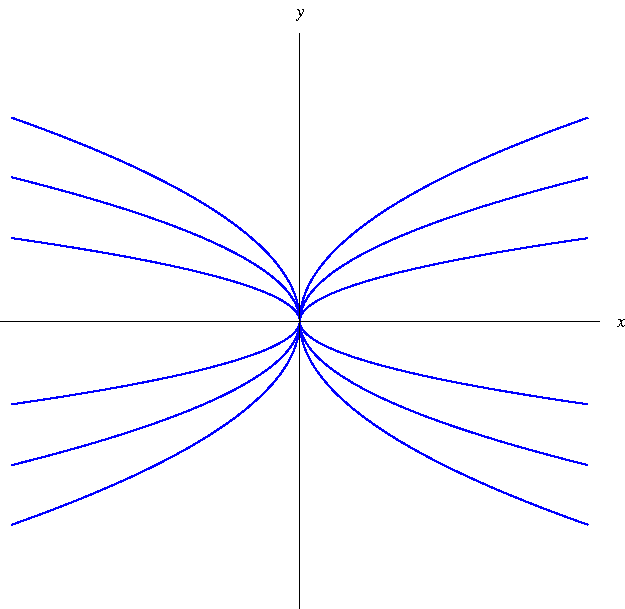
\includegraphics[height=3cm]{diff-eq-separable/pictures/10-03-ex5a.pdf}%
%}%
%\only<11->{%
%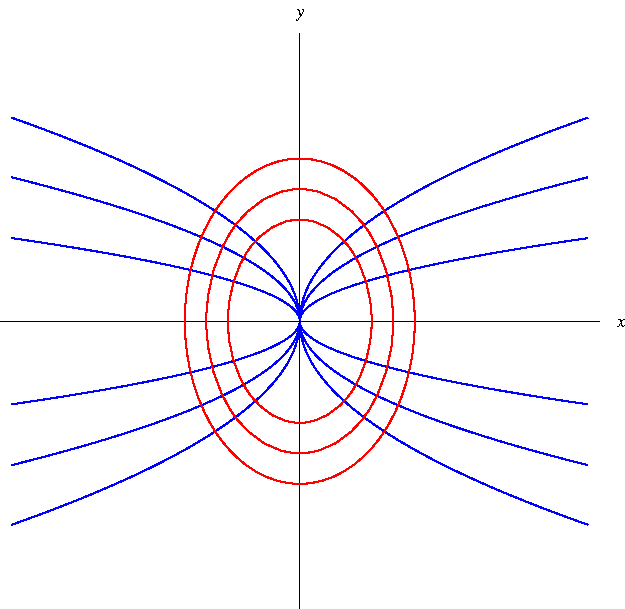
\includegraphics[height=3cm]{diff-eq-separable/pictures/10-03-ex5b.pdf}%
%}%
\end{center}
\column{.5\textwidth}
\uncover<7->{%
An orthogonal trajectory will have a slope that is the negative reciprocal of the slope of the curve.
}%
\abovedisplayskip=0pt
\belowdisplayskip=0pt
\begin{eqnarray*}
\uncover<7->{%
\frac{\diff y}{\diff x}%
}%
& \uncover<7->{ = } &%
\uncover<7->{%
-\frac{2x}{y}%
}\\%
\uncover<8->{%
\int y \diff y%
}%
& \uncover<8->{ = } &%
\uncover<8->{%
-\int 2x\diff x%
}\\%
\uncover<9->{%
\frac{y^2}2%
}%
& \uncover<9->{ = } &%
\uncover<9->{%
-x^2 + C%
}\\%
\uncover<10->{%
x^2 + \frac{y^2}{2} %
}%
& \uncover<10->{ = } &%
\uncover<10->{%
C%
}%
\end{eqnarray*}
\uncover<11->{%
The ellipses $x^2 + \frac{y^2}{2} = C$ are all orthogonal trajectories to $x = ky^2$.
}%
\end{columns}
\end{example}
\end{frame}
% end module orthogonal-trajectory-ex5


%%begin module polar-two-points-coincide-iff
\begin{frame}
\begin{itemize}
\item Let $P_1$ be point  with polar coordinates $(r_1, \theta_1)$.
\item Let $P_2$ be point  with polar coordinates $(r_2, \theta_2)$.
\end{itemize}

\uncover<2->{
\begin{observation}
$P_1$ coincides with $P_2$ if one of the three mutually exclusive possibilities holds:
\begin{itemize}
\item<alert@3> $r_1=r_2\neq 0$ and $\theta_2=\theta_1+2k\pi, k\in \mathbb Z $,
\item<alert@4> $r_1=-r_2\neq 0$ and $\theta_2=\theta_1+(2k+1)\pi, k\in \mathbb Z$,
\item $r_1=r_2=0 $ and $\theta$ is arbitrary.
\end{itemize}
\end{observation}
}
\begin{columns}
\column{.5\textwidth}
\only<3>{
\psset{xunit=2cm, yunit=2cm}
\begin{pspicture}(-0.9, -1.1)(2,0.75) 
\tiny 
%force a boudning box:
%\psline[linecolor=red!1](-0.1, -0.1)(-0.21,0.2)
%\psline[linecolor=red!1](1.1, 0.6)(1.1,0.61)
\psFullDotBlue{0}{0}

%Calculator input: plotCurve{}(1/10 \cos{}t, 1/10 \sin{}t, 0, -3/4 \pi)
\parametricplot[arrows=->, linecolor=\psColorGraph, plotpoints=100]{0} {3.926990817} {t 57.29578 mul cos 0.3000000 mul t 57.29578 mul sin 0.3000000 mul }
\rput[t] (0,-0.1){$O$}
\rput[l](0.3, 0.3){$\theta_1$}

\psline{->}(0,0)(2,0)
\psline[linecolor=blue](0,0)(-0.707106781, -0.707106781)
\psFullDotBlue{-0.707106781}{-0.707106781}
\rput[tl](-0.6, -0.7){$(r_1,\theta_1)$}
\end{pspicture} 
}
\uncover<4>{
\psset{xunit=2cm, yunit=2cm}
\begin{pspicture}(-0.9, -1.1)(2,0.75) 
\tiny 
%force a boudning box:
%\psline[linecolor=red!1](-0.1, -0.1)(-0.21,0.2)
\psline[linecolor=red!1](1.1, 0.5)(1.1,0.51)
\psFullDotBlue{0}{0}

%Calculator input: plotCurve{}(1/10 \cos{}t, 1/10 \sin{}t, 0, -3/4 \pi)
\parametricplot[arrows=->, linecolor=\psColorGraph, plotpoints=100]{0} {-2.35619} {t 57.29578 mul cos 0.3000000 mul t 57.29578 mul sin 0.3000000 mul }
\rput[t] (0,-0.1){$O$}
\rput[l](0.3, -0.2){$\theta_1$}

\psline{->}(0,0)(2,0)
\psline[linecolor=blue](0,0)(-0.707106781, -0.707106781)
\psFullDotBlue{-0.707106781}{-0.707106781}
\rput[tl](-0.6, -0.7){$(r_1,\theta_1)$}
\end{pspicture} 
}

%\ \uncover<1->{%
%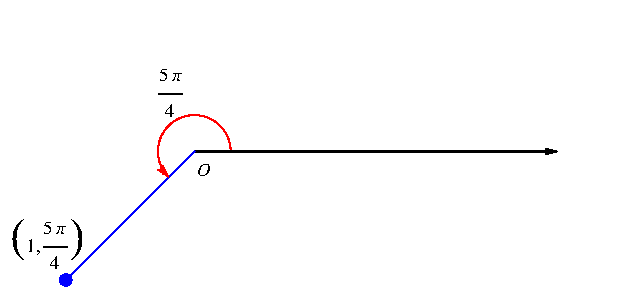
\includegraphics[height=3cm]{polar-curves/pictures/11-03-ex1a.pdf}%
%}%

%\ \uncover<2->{%
%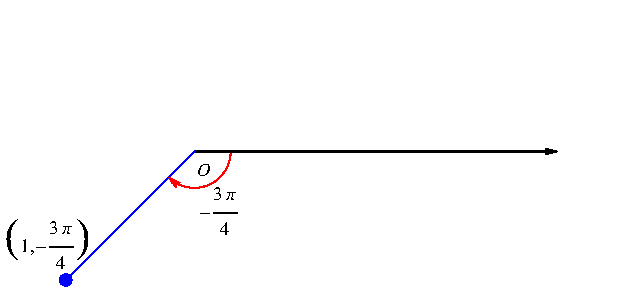
\includegraphics[height=3cm]{polar-curves/pictures/11-03-ex1b.pdf}%
%}%

\vspace{2cm}
\column{.5\textwidth}
\only<3>{
\psset{xunit=2cm, yunit=2cm}
\begin{pspicture}(-0.9, -1.1)(2,0.75) 
\tiny 
%force a boudning box:
%\psline[linecolor=red!1](-0.1, -0.1)(-0.21,0.2)
%\psline[linecolor=red!1](1.1, 0.6)(1.1,0.61)
\psFullDotBlue{0}{0}

%Calculator input: plotCurve{}(1/50 t \cos{}t+3/20 \cos{}t, 1/50 t \sin{}t+3/20 \sin{}t, 0, 13/4 \pi)
\parametricplot[arrows=->, linecolor=\psColorGraph, plotpoints=400] {0} {10.2102} {t 57.29578 mul cos 0.1500000 mul t 57.29578 mul cos t mul 0.0200000 mul add t 57.29578 mul sin 0.1500000 mul t 57.29578 mul sin t mul 0.0200000 mul add }

\rput[t] (0,-0.1){$O$}
\rput[l](0.3, 0.3){$\theta_2=\theta_1+2\pi$}

\psline{->}(0,0)(2,0)
\psline[linecolor=blue](0,0)(-0.707106781, -0.707106781)
\psFullDotBlue{-0.707106781}{-0.707106781}
\rput[tl](-0.6, -0.7){$(r_2, \theta_2)=(r_1,\theta_1+2\pi)$}
\end{pspicture} 
}

\uncover<4>{
\psset{xunit=2cm, yunit=2cm}
\begin{pspicture}(-0.9, -1.1)(2,0.75) 
\tiny 
%force a boudning box:
%\psline[linecolor=red!1](-0.1, -0.1)(-0.21,0.2)
\psline[linecolor=red!1](1.1, 0.5)(1.1,0.51)
\psFullDotBlue{0}{0}

%Calculator input: plotCurve{}(1/10 \cos{}t, 1/10 \sin{}t, 0, -3/4 \pi)
\parametricplot[arrows=->, linecolor=\psColorGraph, plotpoints=100]{0} {0.785398163} {t 57.29578 mul cos 0.3000000 mul t 57.29578 mul sin 0.3000000 mul }
\rput[t] (0,-0.1){$O$}
\rput[l](0.35, 0.15){$\theta_2=\theta_1+\pi$}

\psline{->}(0,0)(2,0)
\psline[linecolor=blue](0,0)(-0.707106781, -0.707106781)
\psFullDotBlue{-0.707106781}{-0.707106781}
\psline[linestyle=dashed](0,0)(0.707106781, 0.707106781)
\psFullDotBlack{0.707106781}{0.707106781}
\rput[tl](-0.6, -0.7){$(r_2, \theta_2)=(-r_1,\theta_1+\pi)$}
\end{pspicture} 
}
%\ \uncover<3->{%
%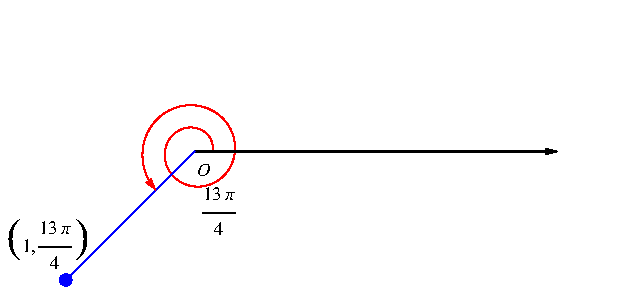
\includegraphics[height=3cm]{polar-curves/pictures/11-03-ex1c.pdf}%
%}%

%\ \uncover<4->{%
%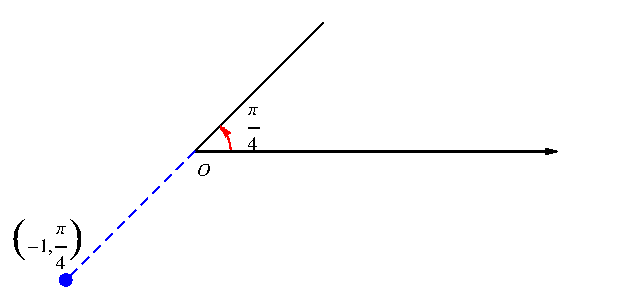
\includegraphics[height=3cm]{polar-curves/pictures/11-03-ex1d.pdf}%
%}%

\vspace{2cm}
\end{columns}
\end{frame}
%end module polar-two-points-coincide-iff


%% begin module cycloid-def
\begin{frame}
\frametitle{The Cycloid}

\psset{xunit=0.8cm, yunit=0.8cm}
\begin{pspicture}(-1.499950, -5)(14.066321,5) 
\psframe*[linecolor=white](-1.499950,-5)(14.066321,5) 
\tiny 

%circles generated by calculator commands:
%precision:=0.99995;f{}{{t}}:=plot2D(\sqrt{1-(x-t)^2}+1, t-precision, t+precision )+plot2D(-\sqrt{1-(x-t)^2}+1, t-precision, t+precision );f{}(0)+f{}(0.5\pi)+f{}(\pi)+f{}(1.5\pi)+f{}(2\pi)+f{}(2.5\pi)+f{}(3\pi)+f{}(3.5\pi)+f{}(4\pi)

\psaxesStandard{-1.1}{-0.5}{13.566321}{2.3}

%calcululator commands: f{}{{t}}:=(DoubleValue (t\pi-sin (t\pi) ), 1-cos (\pi t));(f{}0, f{}0.5, f{}1, f{}1.5, f{}2, f{}2.5, f{}3, f{}3.5, f{}4)
%generate the following points: 
%(0.000000, 0.000000), (0.570796, 1.000000), (3.141593, 2), (5.712389, 1.000000), (6.283185, 0.000000), (6.853982, 1.000000), (9.424778, 2.000000), (11.995574, 1.000000), (12.566371, 0.000000)

\uncover<1>{
%Function formula: (- x^{2}+1)^{1/2}+1 
\psplot[linecolor=\psColorTangent, plotpoints=1000]{-0.999990}{0.999990}{1.0000000 1.0000000 x 2.0000000 exp -1.0000000 mul add 0.5000000 exp add }
%Function formula: - (- x^{2}+1)^{1/2}+1 
\psplot[linecolor=\psColorTangent, plotpoints=1000]{-0.999990}{0.999990}{1.0000000 1.0000000 x 2.0000000 exp -1.0000000 mul add 0.5000000 exp -1.0000000 mul add }
\psFullDot{0}{0}
\rput[bl](0.1, 0.1){$P$}
}

\uncover<2>{
%Function formula: (- (x-1/2 \pi)^{2}+1)^{1/2}+1 
\psplot[linecolor=\psColorTangent, plotpoints=1000]{0.570806}{2.570786}{1.0000000 1.0000000 3.141592654 -0.5000000 mul x add 2.0000000 exp -1.0000000 mul add 0.5000000 exp add }
%Function formula: - (- (x-1/2 \pi)^{2}+1)^{1/2}+1 
\psplot[linecolor=\psColorTangent, plotpoints=1000]{0.570806}{2.570786}{1.0000000 1.0000000 3.141592654 -0.5000000 mul x add 2.0000000 exp -1.0000000 mul add 0.5000000 exp -1.0000000 mul add }
\psFullDot{0.570796}{1}
\rput[l](0.670796, 1.000000){$P$}
}

\uncover<3>{
%Function formula: (- (x- \pi)^{2}+1)^{1/2}+1 
\psplot[linecolor=\psColorTangent, plotpoints=1000]{2.141603}{4.141583}{1.0000000 1.0000000 3.141592654 -1.0000000 mul x add 2.0000000 exp -1.0000000 mul add 0.5000000 exp add }
%Function formula: - (- (x- \pi)^{2}+1)^{1/2}+1 
\psplot[linecolor=\psColorTangent, plotpoints=1000]{2.141603}{4.141583}{1.0000000 1.0000000 3.141592654 -1.0000000 mul x add 2.0000000 exp -1.0000000 mul add 0.5000000 exp -1.0000000 mul add }
\psFullDot{3.141593}{2}
\rput[t](3.141593, 1.9){$P$}
}

\uncover<4>{
%Function formula: (- (x-3/2 \pi)^{2}+1)^{1/2}+1 
\psplot[linecolor=\psColorTangent, plotpoints=1000]{3.712399}{5.712379}{1.0000000 1.0000000 3.141592654 -1.5000000 mul x add 2.0000000 exp -1.0000000 mul add 0.5000000 exp add }
%Function formula: - (- (x-3/2 \pi)^{2}+1)^{1/2}+1 
\psplot[linecolor=\psColorTangent, plotpoints=1000]{3.712399}{5.712379}{1.0000000 1.0000000 3.141592654 -1.5000000 mul x add 2.0000000 exp -1.0000000 mul add 0.5000000 exp -1.0000000 mul add }
\psFullDot{5.712389}{1}
\rput[r](5.612389, 1){$P$}
}

\uncover<5>{
%Function formula: - (- (x-2 \pi)^{2}+1)^{1/2}+1 
\psplot[linecolor=\psColorTangent, plotpoints=1000]{5.283195}{7.283175}{1.0000000 1.0000000 3.141592654 -2.0000000 mul x add 2.0000000 exp -1.0000000 mul add 0.5000000 exp -1.0000000 mul add }
%Function formula: (- (x-2 \pi)^{2}+1)^{1/2}+1 
\psplot[linecolor=\psColorTangent, plotpoints=1000]{5.283195}{7.283175}{1.0000000 1.0000000 3.141592654 -2.0000000 mul x add 2.0000000 exp -1.0000000 mul add 0.5000000 exp add }
\psFullDot{6.283185}{0}
\rput[lb](6.283185, 0.1){$P$}
}

\uncover<6>{
%Function formula: (- (x-5/2 \pi)^{2}+1)^{1/2}+1 
\psplot[linecolor=\psColorTangent, plotpoints=1000]{6.853992}{8.853972}{1.0000000 1.0000000 3.141592654 -2.5000000 mul x add 2.0000000 exp -1.0000000 mul add 0.5000000 exp add }
%Function formula: - (- (x-5/2 \pi)^{2}+1)^{1/2}+1 
\psplot[linecolor=\psColorTangent, plotpoints=1000]{6.853992}{8.853972}{1.0000000 1.0000000 3.141592654 -2.5000000 mul x add 2.0000000 exp -1.0000000 mul add 0.5000000 exp -1.0000000 mul add }
\psFullDot{6.853982}{1}
\rput[l](6.953982, 1.000000){$P$}
}

\uncover<7>{
%Function formula: (- (x-3 \pi)^{2}+1)^{1/2}+1 
\psplot[linecolor=\psColorTangent, plotpoints=1000]{8.424788}{10.424768}{1.0000000 1.0000000 3.141592654 -3.0000000 mul x add 2.0000000 exp -1.0000000 mul add 0.5000000 exp add }
%Function formula: - (- (x-3 \pi)^{2}+1)^{1/2}+1 
\psplot[linecolor=\psColorTangent, plotpoints=1000]{8.424788}{10.424768}{1.0000000 1.0000000 3.141592654 -3.0000000 mul x add 2.0000000 exp -1.0000000 mul add 0.5000000 exp -1.0000000 mul add }
\psFullDot{9.424778}{2}
\rput[t](9.424778, 1.9){$P$}
}

\uncover<8>{
%Function formula: - (- (x-7/2 \pi)^{2}+1)^{1/2}+1 
\psplot[linecolor=\psColorTangent, plotpoints=1000]{9.995584}{11.995564}{1.0000000 1.0000000 3.141592654 -3.5000000 mul x add 2.0000000 exp -1.0000000 mul add 0.5000000 exp -1.0000000 mul add }
%Function formula: (- (x-7/2 \pi)^{2}+1)^{1/2}+1 
\psplot[linecolor=\psColorTangent, plotpoints=1000]{9.995584}{11.995564}{1.0000000 1.0000000 3.141592654 -3.5000000 mul x add 2.0000000 exp -1.0000000 mul add 0.5000000 exp add }
\psFullDot{11.995574}{1}
\rput[r](11.895574, 1.000000){$P$}
}

\uncover<9>{
%Function formula: (- (x-4 \pi)^{2}+1)^{1/2}+1 
\psplot[linecolor=\psColorTangent, plotpoints=1000]{11.566381}{13.566361}{1.0000000 1.0000000 3.141592654 -4.0000000 mul x add 2.0000000 exp -1.0000000 mul add 0.5000000 exp add }
%Function formula: - (- (x-4 \pi)^{2}+1)^{1/2}+1 
\psplot[linecolor=\psColorTangent, plotpoints=1000]{11.566381}{13.566361}{1.0000000 1.0000000 3.141592654 -4.0000000 mul x add 2.0000000 exp -1.0000000 mul add 0.5000000 exp -1.0000000 mul add }
\psFullDot{12.566371}{0}
\rput[lb](12.566371, 0.1){$P$}
}

%Calculator input:f{}{{p}}:=plotCurve(t+\cos(- t+3\pi/2), 1+\sin(3\pi/2- t),p, p+\pi/4)+ plotCurve(t+\cos(- t+3\pi/2), 1+\sin(3\pi/2- t), p+\pi/4, p+\pi/2); f{}0+f{}(0.5\pi)+ f{}(\pi)+f{}(1.5\pi)+f{}(2\pi)+f{}(2.5\pi)+f{}(3\pi)+f{}(3.5\pi)+f{}(4\pi)


\uncover<2->{
%Calculator input: plotCurve{}(\cos{}(- t+3/2 \pi)+t, \sin{}(- t+3/2 \pi)+1, 0, 1/4 \pi)
\parametricplot[linecolor=\psColorGraph, arrows=->, plotpoints=1000]{0}{0.785398}{t 3.141592654 1.5000000 mul t -1.0000000 mul add 57.29578 mul cos add 1.0000000 3.141592654 1.5000000 mul t -1.0000000 mul add 57.29578 mul sin add }
%Calculator input: plotCurve{}(\cos{}(- t+3/2 \pi)+t, \sin{}(- t+3/2 \pi)+1, 1/4 \pi, 1/2 \pi)
\parametricplot[linecolor=\psColorGraph, plotpoints=1000]{ 0.785398}{1.5708}{t 3.141592654 1.5000000 mul t -1.0000000 mul add 57.29578 mul cos add 1.0000000 3.141592654 1.5000000 mul t -1.0000000 mul add 57.29578 mul sin add }
}
\uncover<3->{
%Calculator input: plotCurve{}(\cos{}(- t+3/2 \pi)+t, \sin{}(- t+3/2 \pi)+1, 1/2 \pi, 3/4 \pi)
\parametricplot[linecolor=\psColorGraph, arrows=->, plotpoints=1000]{1.5708}{2.35619}{t 3.141592654 1.5000000 mul t -1.0000000 mul add 57.29578 mul cos add 1.0000000 3.141592654 1.5000000 mul t -1.0000000 mul add 57.29578 mul sin add }
%Calculator input: plotCurve{}(\cos{}(- t+3/2 \pi)+t, \sin{}(- t+3/2 \pi)+1, 3/4 \pi, \pi)
\parametricplot[linecolor=\psColorGraph, plotpoints=1000]{2.35619}{3.14159}{t 3.141592654 1.5000000 mul t -1.0000000 mul add 57.29578 mul cos add 1.0000000 3.141592654 1.5000000 mul t -1.0000000 mul add 57.29578 mul sin add }
}
\uncover<4->{
%Calculator input: plotCurve{}(\cos{}(- t+3/2 \pi)+t, \sin{}(- t+3/2 \pi)+1, \pi, 5/4 \pi)
\parametricplot[linecolor=\psColorGraph, arrows=->, plotpoints=1000]{3.14159}{3.92699}{t 3.141592654 1.5000000 mul t -1.0000000 mul add 57.29578 mul cos add 1.0000000 3.141592654 1.5000000 mul t -1.0000000 mul add 57.29578 mul sin add }
%Calculator input: plotCurve{}(\cos{}(- t+3/2 \pi)+t, \sin{}(- t+3/2 \pi)+1, 5/4 \pi, 3/2 \pi)
\parametricplot[linecolor=\psColorGraph, plotpoints=1000]{3.92699}{4.71239}{t 3.141592654 1.5000000 mul t -1.0000000 mul add 57.29578 mul cos add 1.0000000 3.141592654 1.5000000 mul t -1.0000000 mul add 57.29578 mul sin add }
}
\uncover<5->{
%Calculator input: plotCurve{}(\cos{}(- t+3/2 \pi)+t, \sin{}(- t+3/2 \pi)+1, 3/2 \pi, 7/4 \pi)
\parametricplot[linecolor=\psColorGraph, arrows=->, plotpoints=1000]{4.71239}{5.49779}{t 3.141592654 1.5000000 mul t -1.0000000 mul add 57.29578 mul cos add 1.0000000 3.141592654 1.5000000 mul t -1.0000000 mul add 57.29578 mul sin add }
%Calculator input: plotCurve{}(\cos{}(- t+3/2 \pi)+t, \sin{}(- t+3/2 \pi)+1, 7/4 \pi, 2 \pi)
\parametricplot[linecolor=\psColorGraph, plotpoints=1000]{5.49779}{6.28319}{t 3.141592654 1.5000000 mul t -1.0000000 mul add 57.29578 mul cos add 1.0000000 3.141592654 1.5000000 mul t -1.0000000 mul add 57.29578 mul sin add }
}
\uncover<6->{
%Calculator input: plotCurve{}(\cos{}(- t+3/2 \pi)+t, \sin{}(- t+3/2 \pi)+1, 2 \pi, 9/4 \pi)
\parametricplot[linecolor=\psColorGraph, arrows=->, plotpoints=1000]{6.28319}{7.06858}{t 3.141592654 1.5000000 mul t -1.0000000 mul add 57.29578 mul cos add 1.0000000 3.141592654 1.5000000 mul t -1.0000000 mul add 57.29578 mul sin add }
%Calculator input: plotCurve{}(\cos{}(- t+3/2 \pi)+t, \sin{}(- t+3/2 \pi)+1, 9/4 \pi, 5/2 \pi)
\parametricplot[linecolor=\psColorGraph, plotpoints=1000]{7.06858}{7.85398}{t 3.141592654 1.5000000 mul t -1.0000000 mul add 57.29578 mul cos add 1.0000000 3.141592654 1.5000000 mul t -1.0000000 mul add 57.29578 mul sin add }
}
\uncover<7->{
%Calculator input: plotCurve{}(\cos{}(- t+3/2 \pi)+t, \sin{}(- t+3/2 \pi)+1, 5/2 \pi, 11/4 \pi)
\parametricplot[linecolor=\psColorGraph, arrows=->, plotpoints=1000]{7.85398}{8.63938}{t 3.141592654 1.5000000 mul t -1.0000000 mul add 57.29578 mul cos add 1.0000000 3.141592654 1.5000000 mul t -1.0000000 mul add 57.29578 mul sin add }
%Calculator input: plotCurve{}(\cos{}(- t+3/2 \pi)+t, \sin{}(- t+3/2 \pi)+1, 11/4 \pi, 3 \pi)
\parametricplot[linecolor=\psColorGraph, plotpoints=1000]{8.63938}{9.42478}{t 3.141592654 1.5000000 mul t -1.0000000 mul add 57.29578 mul cos add 1.0000000 3.141592654 1.5000000 mul t -1.0000000 mul add 57.29578 mul sin add }
}
\uncover<8->{
%Calculator input: plotCurve{}(\cos{}(- t+3/2 \pi)+t, \sin{}(- t+3/2 \pi)+1, 3 \pi, 13/4 \pi)
\parametricplot[linecolor=\psColorGraph, arrows=->, plotpoints=1000]{9.42478}{10.2102}{t 3.141592654 1.5000000 mul t -1.0000000 mul add 57.29578 mul cos add 1.0000000 3.141592654 1.5000000 mul t -1.0000000 mul add 57.29578 mul sin add }
%Calculator input: plotCurve{}(\cos{}(- t+3/2 \pi)+t, \sin{}(- t+3/2 \pi)+1, 13/4 \pi, 7/2 \pi)
\parametricplot[linecolor=\psColorGraph, plotpoints=1000]{10.2102}{10.9956}{t 3.141592654 1.5000000 mul t -1.0000000 mul add 57.29578 mul cos add 1.0000000 3.141592654 1.5000000 mul t -1.0000000 mul add 57.29578 mul sin add }
}
\uncover<9->{
%Calculator input: plotCurve{}(\cos{}(- t+3/2 \pi)+t, \sin{}(- t+3/2 \pi)+1, 7/2 \pi, 15/4 \pi)
\parametricplot[linecolor=\psColorGraph, arrows=->, plotpoints=1000]{10.9956}{11.781}{t 3.141592654 1.5000000 mul t -1.0000000 mul add 57.29578 mul cos add 1.0000000 3.141592654 1.5000000 mul t -1.0000000 mul add 57.29578 mul sin add }
%Calculator input: plotCurve{}(\cos{}(- t+3/2 \pi)+t, \sin{}(- t+3/2 \pi)+1, 15/4 \pi, 4 \pi)
\parametricplot[linecolor=\psColorGraph, plotpoints=1000]{11.781}{12.5664}{t 3.141592654 1.5000000 mul t -1.0000000 mul add 57.29578 mul cos add 1.0000000 3.141592654 1.5000000 mul t -1.0000000 mul add 57.29578 mul sin add }
}
\uncover<10->{
%Calculator input: plotCurve{}(\cos{}(- t+3/2 \pi)+t, \sin{}(- t+3/2 \pi)+1, 4 \pi, 17/4 \pi)
\parametricplot[linecolor=\psColorGraph, arrows=->, plotpoints=1000]{12.5664}{13.3518}{t 3.141592654 1.5000000 mul t -1.0000000 mul add 57.29578 mul cos add 1.0000000 3.141592654 1.5000000 mul t -1.0000000 mul add 57.29578 mul sin add }
%Calculator input: plotCurve{}(\cos{}(- t+3/2 \pi)+t, \sin{}(- t+3/2 \pi)+1, 17/4 \pi, 9/2 \pi)
\parametricplot[linecolor=\psColorGraph, plotpoints=1000]{13.3518}{14.1372}{t 3.141592654 1.5000000 mul t -1.0000000 mul add 57.29578 mul cos add 1.0000000 3.141592654 1.5000000 mul t -1.0000000 mul add 57.29578 mul sin add }
}
\end{pspicture} 


%\ \only<handout:0| 1>{%
%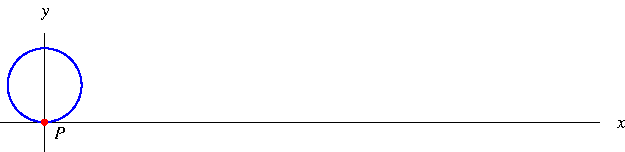
\includegraphics[width=12cm]{parametric-curves/pictures/11-01-cycloida.pdf}%
%}%
%\only<handout:0| 2>{%
%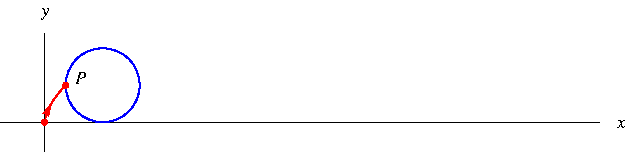
\includegraphics[width=12cm]{parametric-curves/pictures/11-01-cycloidb.pdf}%
%}%
%\only<handout:0| 3>{%
%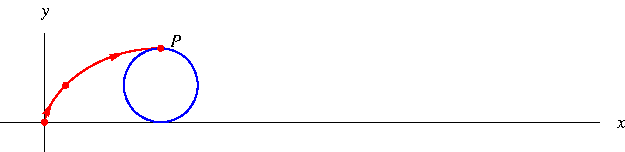
\includegraphics[width=12cm]{parametric-curves/pictures/11-01-cycloidc.pdf}%
%}%
%\only<handout:0| 4>{%
%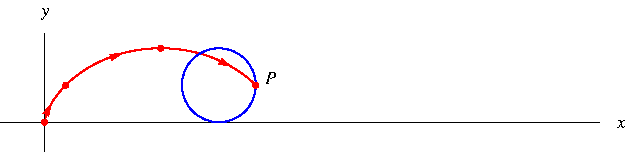
\includegraphics[width=12cm]{parametric-curves/pictures/11-01-cycloidd.pdf}%
%}%
%\only<handout:0| 5>{%
%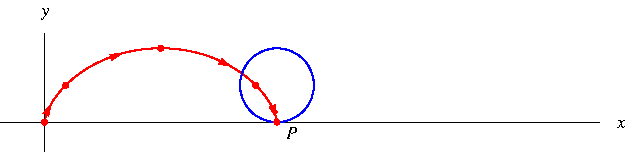
\includegraphics[width=12cm]{parametric-curves/pictures/11-01-cycloide.pdf}%
%}%
%\only<handout:0| 6>{%
%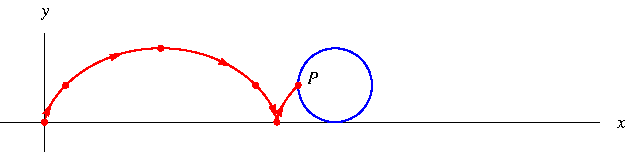
\includegraphics[width=12cm]{parametric-curves/pictures/11-01-cycloidf.pdf}%
%}%
%\only<handout:0| 7>{%
%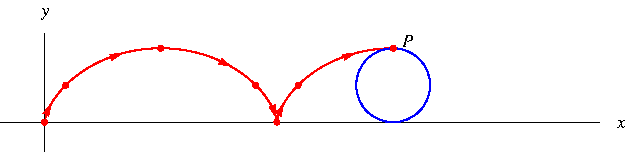
\includegraphics[width=12cm]{parametric-curves/pictures/11-01-cycloidg.pdf}%
%}%
%\only<8>{%
%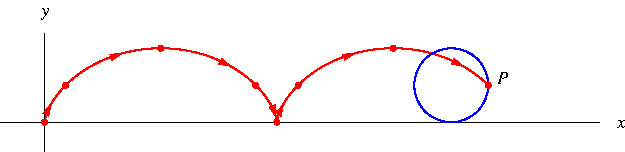
\includegraphics[width=12cm]{parametric-curves/pictures/11-01-cycloidh.pdf}%
%}%
%\only<handout:0| 9>{%
%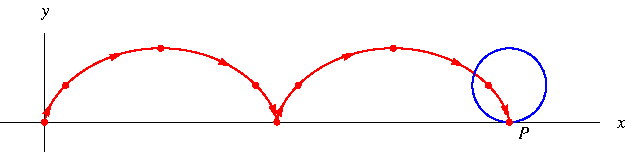
\includegraphics[width=12cm]{parametric-curves/pictures/11-01-cycloidi.pdf}%
%}%
%\only<handout:0| 10->{%
%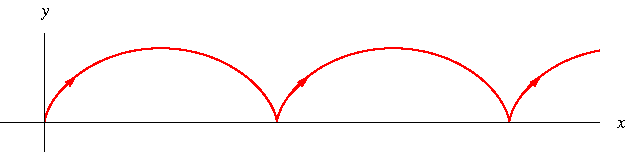
\includegraphics[width=12cm]{parametric-curves/pictures/11-01-cycloidj.pdf}%
%}%
\begin{definition}[Cycloid]
The curve traced out by a point $P$ on the circumference of a circle as the circle rolls along a straight line is called a cycloid. \uncover<10>{}
\end{definition}
\end{frame}
% end module cycloid-def

%%begin module polar-two-points-coincide-iff
\begin{frame}
\begin{itemize}
\item Let $P_1$ be point  with polar coordinates $(r_1, \theta_1)$.
\item Let $P_2$ be point  with polar coordinates $(r_2, \theta_2)$.
\end{itemize}

\uncover<2->{
\begin{observation}
$P_1$ coincides with $P_2$ if one of the three mutually exclusive possibilities holds:
\begin{itemize}
\item<alert@3> $r_1=r_2\neq 0$ and $\theta_2=\theta_1+2k\pi, k\in \mathbb Z $,
\item<alert@4> $r_1=-r_2\neq 0$ and $\theta_2=\theta_1+(2k+1)\pi, k\in \mathbb Z$,
\item $r_1=r_2=0 $ and $\theta$ is arbitrary.
\end{itemize}
\end{observation}
}
\begin{columns}
\column{.5\textwidth}
\only<3>{
\psset{xunit=2cm, yunit=2cm}
\begin{pspicture}(-0.9, -1.1)(2,0.75) 
\tiny 
%force a boudning box:
%\psline[linecolor=red!1](-0.1, -0.1)(-0.21,0.2)
%\psline[linecolor=red!1](1.1, 0.6)(1.1,0.61)
\psFullDotBlue{0}{0}

%Calculator input: plotCurve{}(1/10 \cos{}t, 1/10 \sin{}t, 0, -3/4 \pi)
\parametricplot[arrows=->, linecolor=\psColorGraph, plotpoints=100]{0} {3.926990817} {t 57.29578 mul cos 0.3000000 mul t 57.29578 mul sin 0.3000000 mul }
\rput[t] (0,-0.1){$O$}
\rput[l](0.3, 0.3){$\theta_1$}

\psline{->}(0,0)(2,0)
\psline[linecolor=blue](0,0)(-0.707106781, -0.707106781)
\psFullDotBlue{-0.707106781}{-0.707106781}
\rput[tl](-0.6, -0.7){$(r_1,\theta_1)$}
\end{pspicture} 
}
\uncover<4>{
\psset{xunit=2cm, yunit=2cm}
\begin{pspicture}(-0.9, -1.1)(2,0.75) 
\tiny 
%force a boudning box:
%\psline[linecolor=red!1](-0.1, -0.1)(-0.21,0.2)
\psline[linecolor=red!1](1.1, 0.5)(1.1,0.51)
\psFullDotBlue{0}{0}

%Calculator input: plotCurve{}(1/10 \cos{}t, 1/10 \sin{}t, 0, -3/4 \pi)
\parametricplot[arrows=->, linecolor=\psColorGraph, plotpoints=100]{0} {-2.35619} {t 57.29578 mul cos 0.3000000 mul t 57.29578 mul sin 0.3000000 mul }
\rput[t] (0,-0.1){$O$}
\rput[l](0.3, -0.2){$\theta_1$}

\psline{->}(0,0)(2,0)
\psline[linecolor=blue](0,0)(-0.707106781, -0.707106781)
\psFullDotBlue{-0.707106781}{-0.707106781}
\rput[tl](-0.6, -0.7){$(r_1,\theta_1)$}
\end{pspicture} 
}

%\ \uncover<1->{%
%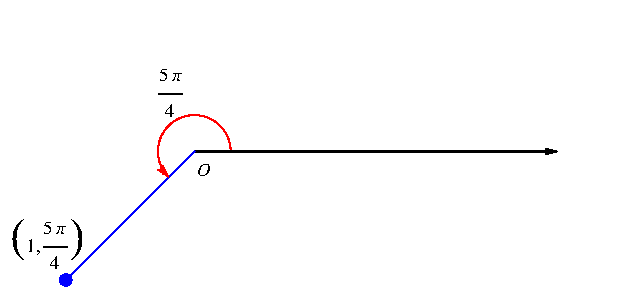
\includegraphics[height=3cm]{polar-curves/pictures/11-03-ex1a.pdf}%
%}%

%\ \uncover<2->{%
%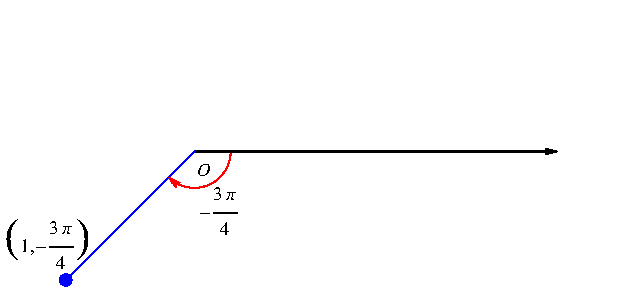
\includegraphics[height=3cm]{polar-curves/pictures/11-03-ex1b.pdf}%
%}%

\vspace{2cm}
\column{.5\textwidth}
\only<3>{
\psset{xunit=2cm, yunit=2cm}
\begin{pspicture}(-0.9, -1.1)(2,0.75) 
\tiny 
%force a boudning box:
%\psline[linecolor=red!1](-0.1, -0.1)(-0.21,0.2)
%\psline[linecolor=red!1](1.1, 0.6)(1.1,0.61)
\psFullDotBlue{0}{0}

%Calculator input: plotCurve{}(1/50 t \cos{}t+3/20 \cos{}t, 1/50 t \sin{}t+3/20 \sin{}t, 0, 13/4 \pi)
\parametricplot[arrows=->, linecolor=\psColorGraph, plotpoints=400] {0} {10.2102} {t 57.29578 mul cos 0.1500000 mul t 57.29578 mul cos t mul 0.0200000 mul add t 57.29578 mul sin 0.1500000 mul t 57.29578 mul sin t mul 0.0200000 mul add }

\rput[t] (0,-0.1){$O$}
\rput[l](0.3, 0.3){$\theta_2=\theta_1+2\pi$}

\psline{->}(0,0)(2,0)
\psline[linecolor=blue](0,0)(-0.707106781, -0.707106781)
\psFullDotBlue{-0.707106781}{-0.707106781}
\rput[tl](-0.6, -0.7){$(r_2, \theta_2)=(r_1,\theta_1+2\pi)$}
\end{pspicture} 
}

\uncover<4>{
\psset{xunit=2cm, yunit=2cm}
\begin{pspicture}(-0.9, -1.1)(2,0.75) 
\tiny 
%force a boudning box:
%\psline[linecolor=red!1](-0.1, -0.1)(-0.21,0.2)
\psline[linecolor=red!1](1.1, 0.5)(1.1,0.51)
\psFullDotBlue{0}{0}

%Calculator input: plotCurve{}(1/10 \cos{}t, 1/10 \sin{}t, 0, -3/4 \pi)
\parametricplot[arrows=->, linecolor=\psColorGraph, plotpoints=100]{0} {0.785398163} {t 57.29578 mul cos 0.3000000 mul t 57.29578 mul sin 0.3000000 mul }
\rput[t] (0,-0.1){$O$}
\rput[l](0.35, 0.15){$\theta_2=\theta_1+\pi$}

\psline{->}(0,0)(2,0)
\psline[linecolor=blue](0,0)(-0.707106781, -0.707106781)
\psFullDotBlue{-0.707106781}{-0.707106781}
\psline[linestyle=dashed](0,0)(0.707106781, 0.707106781)
\psFullDotBlack{0.707106781}{0.707106781}
\rput[tl](-0.6, -0.7){$(r_2, \theta_2)=(-r_1,\theta_1+\pi)$}
\end{pspicture} 
}
%\ \uncover<3->{%
%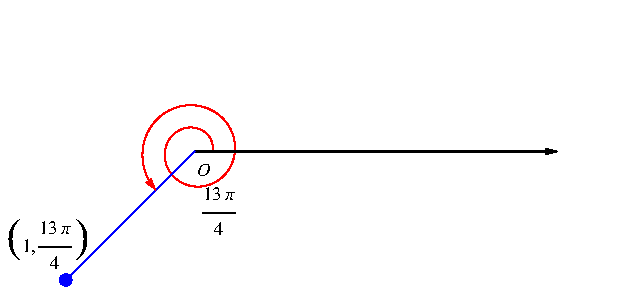
\includegraphics[height=3cm]{polar-curves/pictures/11-03-ex1c.pdf}%
%}%

%\ \uncover<4->{%
%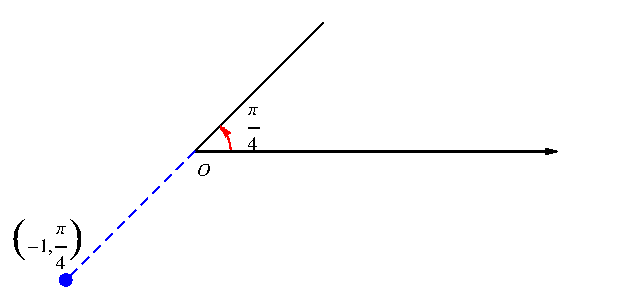
\includegraphics[height=3cm]{polar-curves/pictures/11-03-ex1d.pdf}%
%}%

\vspace{2cm}
\end{columns}
\end{frame}
%end module polar-two-points-coincide-iff

%% begin module polar-intersection-ex3
\begin{frame}
\begin{example} %[Example 3, p. 688]
Find all points of intersection of the polar curves $r = \frac{1}{2}$ and $r = \cos (2\theta)$.
\begin{columns}[c]
\column{.4\textwidth}

\psset{xunit=1.8cm, yunit=1.8cm}
\begin{pspicture}(-1.5, -1.5)(1.5,1.5)
\tiny
\fcAxesStandard{-1.4}{-1.4}{1.4}{1.4}
%Calculator command: drawPolar{}(1/2, 0, 2 \pi)
\parametricplot[linecolor=\fcColorGraph, plotpoints=1000, algebraic=false]{0}{6.28319}{ 0.5 t 57.29578 mul cos mul 0.5 t 57.29578 mul sin mul }
%Calculator command: drawPolar{}(\cos{}(2 t), 0, 2 \pi)
\parametricplot[linecolor=\fcColorGraph, plotpoints=1000, algebraic=false]{0}{6.28319}{t 2 mul 57.29578 mul cos t 57.29578 mul cos mul t 2 mul 57.29578 mul cos t 57.29578 mul sin mul }

\rput[tr](-0.8, -0.8){$r=\frac{1}{2}$}
\psline{->}(-0.75, -0.75)(-0.353553391, -0.353553391)
\rput[lt] (0.2, -1){$r=\cos (2\theta)$}

\uncover<4->{
\fcFullDotBlack{0.433013}{0.25}
\fcFullDotBlack{-0.433013}{0.25}
\fcFullDotBlack{-0.433013}{-0.25}
\fcFullDotBlack{0.433013}{-0.25}
}
\uncover<6->{
\fcFullDotBlack{0.25}{0.433013}
\fcFullDotBlack{0.25}{-0.433013}
\fcFullDotBlack{-0.25}{-0.433013}
\fcFullDotBlack{-0.25}{0.433013}
}
\uncover<9>{
\pscircle*[linecolor=red](0.433013,0.25){0.09}
\pscircle*[linecolor=red](-0.433013,0.25){0.09}
\pscircle*[linecolor=red](-0.433013,-0.25){0.09}
\pscircle*[linecolor=red](0.433013,-0.25){0.09}
}
\uncover<10>{
\pscircle*[linecolor=red](0.25,0.433013){0.09}
\pscircle*[linecolor=red](0.25,-0.433013){0.09}
\pscircle*[linecolor=red](-0.25,-0.433013){0.09}
\pscircle*[linecolor=red](-0.25,0.433013){0.09}
}
\end{pspicture}

%\ \only<handout:0| -3>{%
%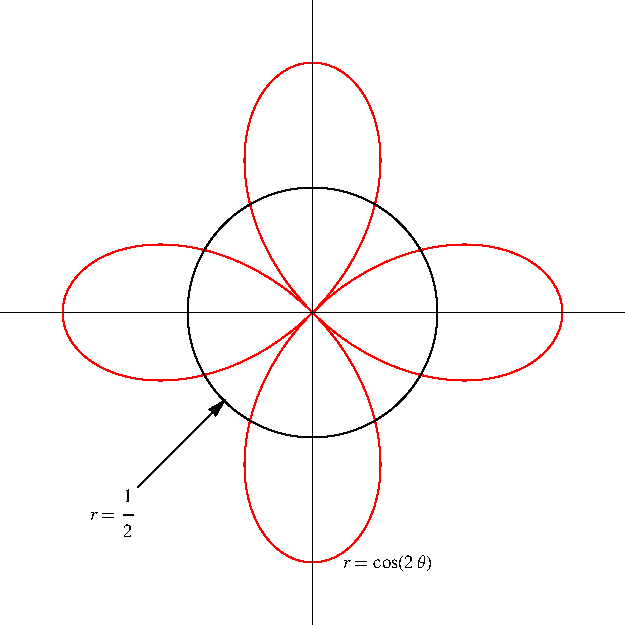
\includegraphics[height=5cm]{polar-curves/pictures/11-04-ex3a.pdf}%
%}%
%\only<handout:0| 4-5>{%
%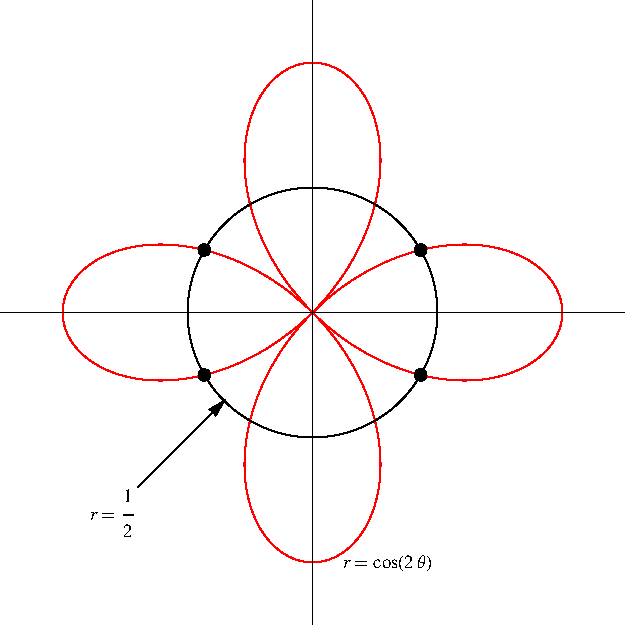
\includegraphics[height=5cm]{polar-curves/pictures/11-04-ex3b.pdf}%
%}%
%\only<6-8>{%
%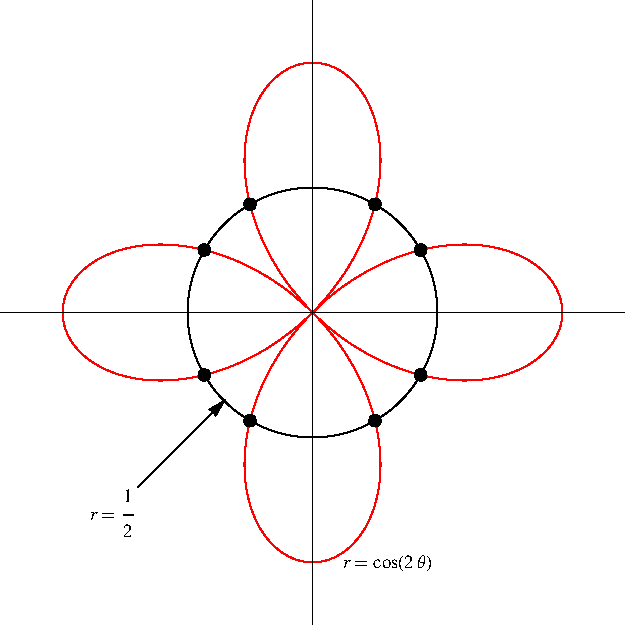
\includegraphics[height=5cm]{polar-curves/pictures/11-04-ex3c.pdf}%
%}%
%\only<handout:0| 9>{%
%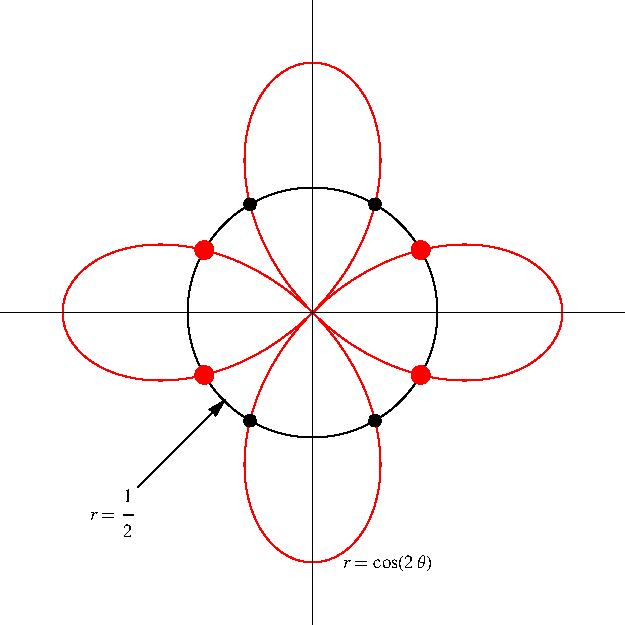
\includegraphics[height=5cm]{polar-curves/pictures/11-04-ex3d.pdf}%
%}%
%\only<handout:0| 10->{%
%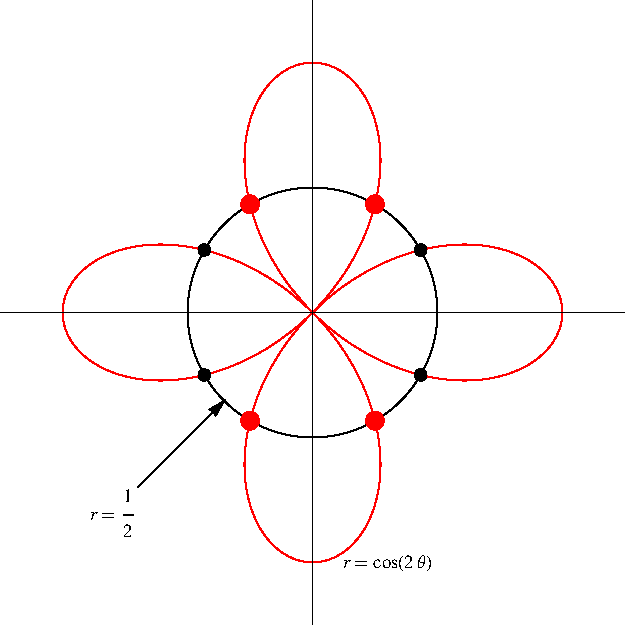
\includegraphics[height=5cm]{polar-curves/pictures/11-04-ex3e.pdf}%
%}%
\column{.6\textwidth}
\abovedisplayskip=0pt
\belowdisplayskip=0pt
\begin{eqnarray*}
\uncover<2->{%
\cos 2\theta%
}%
& \uncover<2->{ = } &%
\uncover<2->{%
\frac{1}{2}%
}\\%
\uncover<3->{%
2\theta%
}%
& \uncover<3->{ = } &%
\uncover<3->{%
\frac{\pi}{3}, \frac{5\pi}{3}, \frac{7\pi}{3}, \frac{11\pi}{3}%
}\\%
\uncover<4->{%
\theta%
}%
& \uncover<4->{ = } &%
\uncover<4->{%
\frac{\pi}{6}, \frac{5\pi}{6}, \frac{7\pi}{6}, \frac{11\pi}{6}%
}%
\end{eqnarray*}
\begin{itemize}
\item<5->  This only gives four points.
\item<6->  There are actually eight.
\item<7->  The circle $r = \frac{1}{2}$ also has polar equation $r = -\frac{1}{2}$.
\item<8->  To find all eight points, solve \alertNoH{ 9}{$\cos (2\theta )= \frac{1}{2}$} and \alertNoH{ 10}{$\cos (2\theta) = -\frac{1}{2}$}.
\end{itemize}
\end{columns}
\end{example}
\end{frame}
% end module polar-intersection-ex3


%% begin module trig-substitutions-ex3
\begin{frame}
\begin{example} %[Example 3, p. 505]
\begin{columns}[c]
\column{.4\textwidth}
Find $\int \frac{1}{x^2 \sqrt{x^2+4}}\diff x$.
\begin{itemize}
\item<2->  Let \alert<handout:0| 3-4,7,14,20>{$x = \uncover<4->{2\tan \theta}$}\uncover<4->{, where \alert<handout:0| 10>{$-\pi /2 \leq \theta \leq \pi / 2$}.}
\item<2->  Then \alert<handout:0| 5-6,13>{$\diff x = \uncover<6->{2\sec^2 \theta\diff \theta}$}\uncover<6->{.}
\end{itemize}
\column{.6\textwidth}
\begin{center}
\psset{xunit=2cm, yunit=2cm}
\begin{pspicture}(-0.15,-0.3)(2.3,1.2)
\psframe*[linecolor=white](-0.1,-0.3)(2.3,1.2)
\psline(0,0)(2, 0)(2,1)(0,0)
\psline(1.9,0)(1.9, 0.1)(2,0.1)
\psAngle{0}{0.463648}{0.4}{$\theta$}
\uncover<handout:0|20->{
\rput[l](2.1, 0.5){$x$}
\rput[t](1, -0.1){$2$}
}
\uncover<handout:0|21->{
\rput[br](1, 0.55){$\sqrt{x^2+4}$}
}
%bounding box for pdflatex compilation:
\psline[linecolor=red!1](-0.11, -0.3 )(-0.105, -0.3)
\psline[linecolor=red!1](2.3, 1.21)(2.3, 1.205)
\end{pspicture}
%\ \only<handout:0| -19>{%
%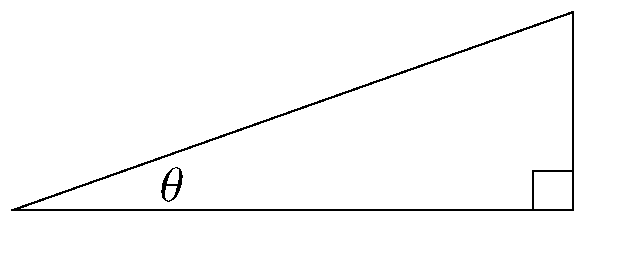
\includegraphics[height=3cm]{trig-substitution/pictures/08-03-ex3a.pdf}%
%}%
%\only<handout:0| 20>{%
%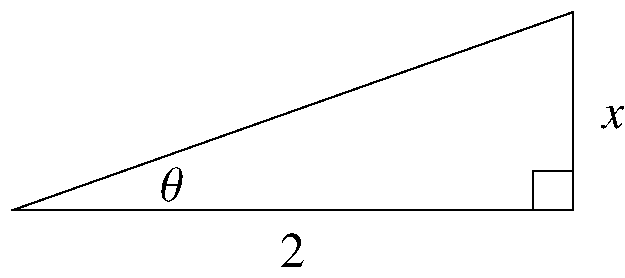
\includegraphics[height=3cm]{trig-substitution/pictures/08-03-ex3b.pdf}%
%}%
%\only<21->{%
%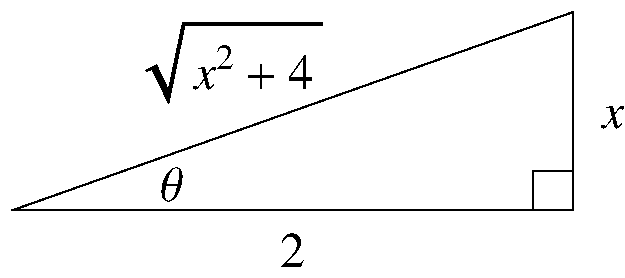
\includegraphics[height=3cm]{trig-substitution/pictures/08-03-ex3c.pdf}%
%}%
\end{center}
\end{columns}
\abovedisplayskip=0pt
\belowdisplayskip=0pt
\[
\uncover<2->{%
\alert<handout:0| 12>{%
\sqrt{\alert<handout:0| 7>{x^2} + 4} = 
}%
}%
\uncover<7->{%
\sqrt{\alert<handout:0| 7>{4\tan^2 \theta} + 4} = 
}%
\uncover<8->{%
\sqrt{4 \sec^2 \theta} = 
}%
\uncover<9->{%
2 |\sec  \theta | = 
}%
\uncover<10->{%
\alert<handout:0| 12>{%
2 \sec  \theta  
}%
}%
\]
\abovedisplayskip=0pt
\belowdisplayskip=0pt
\begin{eqnarray*}
\uncover<11->{%
\int \frac{\alert<handout:0| 13>{\diff x}}{\alert<handout:0| 14>{x^2}\alert<handout:0| 12>{\sqrt{x^2+4}}}%
}%
& \uncover<11->{ = } & %
\uncover<11->{%
\int\frac{\alert<handout:0| 13>{2\sec^2 \theta \diff \theta}}{\alert<handout:0| 14>{4\tan^2 \theta}\cdot \alert<handout:0| 12>{2\sec \theta}}
}%
\uncover<15->{%
 = \frac{1}{4}\int \frac{\cos \theta}{\sin^2\theta} \diff \theta
}\\%
\uncover<16->{%
\textrm{Let } \alert<handout:0| 19>{u = \sin \theta} :%
}%
& \uncover<17->{ = } & %
\uncover<17->{%
\frac{1}{4} \int \frac{\diff u}{u^2}
}  \uncover<18->{ = }  \uncover<18->{%
\frac{1}{4} \left( -\alert<handout:0| 19>{\frac{1}{u}}\right)  + C
}\\%
& \uncover<19->{ = } & %
\uncover<19->{%
 -\frac{\alert<handout:0| 19,22-23>{\csc \theta}}{4} + C
}%
\uncover<23->{%
=  -\frac{\alert<handout:0| 23>{\sqrt{x^2+4}}}{4\alert<handout:0| 23>{x}} + C
}%
\end{eqnarray*}
\end{example}
\end{frame}
% end module trig-substitutions-ex3

%% begin module trig-substitutions-ex1
\begin{frame}
\begin{example} %[Example 1, p. 504]
\begin{columns}[c]
\column{.4\textwidth}
Evaluate $\int \frac{\sqrt{9-x^2}}{x^2}\diff x$.
\begin{itemize}
\item<2->  Let \alert<handout:0| 3-4,7,14,18>{$x = \uncover<4->{3\sin \theta}$}\uncover<4->{, where \alert<handout:0| 10>{$-\pi /2 \leq \theta \leq \pi / 2$}.}
\item<2->  Then \alert<handout:0| 5-6,13>{$\diff x = \uncover<6->{3\cos \theta\diff \theta}$}\uncover<6->{.}
\end{itemize}
\column{.6\textwidth}
\psset{xunit=1.5cm, yunit=1.5cm}
\begin{pspicture}(-0.15,-0.4)(3.3,1.2)
\psframe*[linecolor=white](-0.1,-0.4)(3.3,1.2)
\psline(0,0)(3, 0)(3,1)(0,0)
\psline(2.9,0)(2.9, 0.1)(3,0.1)
\fcAngle{0}{0.339837}{0.6}{$\theta$}
\uncover<handout:0|18->{
\rput[l](3.1, 0.5){$x$}
\rput[br](1.5, 0.55){$3$}
}
\uncover<handout:0|19->{
\rput[t](1.5, -0.1){$\sqrt{9-x^2} $}
}
%bounding box for pdflatex compilation:
\psline[linecolor=red!1](-0.11, -0.4 )(-0.105, -0.4)
\psline[linecolor=red!1](3.3, 1.21)(3.3, 1.205)
\end{pspicture}
%\ \only<handout:0| -17>{%
%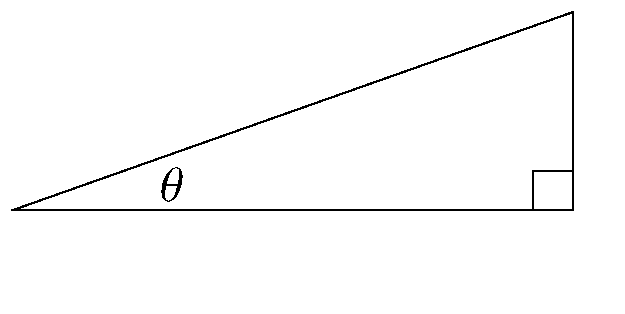
\includegraphics[height=3cm]{trig-substitution/pictures/08-03-ex1a.pdf}%
%}%
%\only<handout:0| 18>{%
%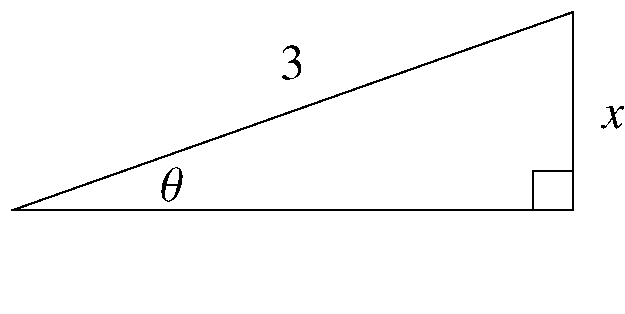
\includegraphics[height=3cm]{trig-substitution/pictures/08-03-ex1b.pdf}%
%}%
%\only<19->{%
%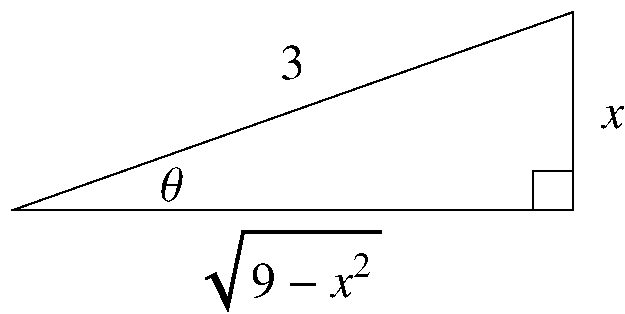
\includegraphics[height=3cm]{trig-substitution/pictures/08-03-ex1c.pdf}%
%}%
\end{columns}
\abovedisplayskip=0pt
\belowdisplayskip=0pt
\[
\uncover<2->{%
\alert<handout:0| 12>{%
\sqrt{9 - \alert<handout:0| 7>{x^2}} =
}%
}%
\uncover<7->{%
\sqrt{9 - \alert<handout:0| 7>{9\sin^2 \theta}} =
}%
\uncover<8->{%
\sqrt{9 \cos^2 \theta} =
}%
\uncover<9->{%
3 |\cos  \theta | =
}%
\uncover<10->{%
\alert<handout:0| 12>{%
3 \cos  \theta
}%
}%
\]
\abovedisplayskip=0pt
\belowdisplayskip=0pt
\begin{eqnarray*}
\uncover<11->{%
\int \frac{\alert<handout:0| 12>{\sqrt{9-x^2}}}{\alert<handout:0| 14>{x^2}}\alert<handout:0| 13>{\diff x}%
}%
& \uncover<11->{ = } & %
\uncover<11->{%
\int\frac{\alert<handout:0| 12>{3\cos \theta}}{\alert<handout:0| 14>{9\sin^2 \theta}}\alert<handout:0| 13>{3\cos \theta \diff \theta}
}%
\uncover<15->{%
 = \int \cot^2 \theta \diff \theta
}\\%
& \uncover<16->{ = } & %
\uncover<16->{%
 \int (\csc^2 \theta  - 1)\diff \theta
}  \uncover<17->{ = }  \uncover<17->{%
 -\alert<handout:0| 20-21>{\cot \theta} - \theta + C
}\\%
& \uncover<21->{ = } & %
\uncover<21->{%
 -\alert<handout:0| 21>{\frac{\sqrt{9-x^2}}{x}} - \Arcsin \left( \frac{x}{3}\right) + C
}%
\end{eqnarray*}
\end{example}
\end{frame}
% end module trig-substitutions-ex1

%% begin module trig-substitutions-ex5
\begin{frame}
\begin{example} %[Example 5, p. 506]
\begin{columns}[c]
\column{.4\textwidth}
Find $\int \frac{\diff x}{\sqrt{x^2-a^2}}$, \alert<handout:0| 9>{$a > 0$}.
\begin{itemize}
\item<2->  \alert<handout:0| 3-4,7,16,20>{$x = \uncover<4->{a\sec \theta}$}\uncover<4->{,  \alert<handout:0| 10>{$0 < \theta < \pi / 2$ or $\pi < \theta < 3\pi /2$}.}
\item<2->  \alert<handout:0| 5-6,13>{$\diff x = \uncover<6->{a\sec \theta\tan \theta \diff \theta}$}\uncover<6->{.}
\end{itemize}
\column{.6\textwidth}
\psset{xunit=1.5cm, yunit=1.5cm}
\begin{pspicture}(-0.15,-0.4)(4.4,1.2)
\psframe*[linecolor=white](-0.1,-0.4)(4.4,1.2)
\psline(0,0)(3, 0)(3,1)(0,0)
\psline(2.9,0)(2.9, 0.1)(3,0.1)
\fcAngle{0}{0.339837}{0.6}{$\theta$}
\uncover<handout:0|16->{
\rput[br](1.5, 0.55){$x$}
\rput[t](1.5, -0.1){$a$}
}
\uncover<handout:0|17->{
\rput[l](3.1, 0.5){$\sqrt{x^2-a^2}$}
}
%bounding box for pdflatex compilation:
\psline[linecolor=red!1](-0.11, -0.4 )(-0.105, -0.4)
\psline[linecolor=red!1](4.4, 1.21)(4.4, 1.205)
\end{pspicture}
\end{columns}
\abovedisplayskip=0pt
\belowdisplayskip=0pt
\[
\uncover<2->{%
\alert<handout:0| 12>{%
\sqrt{\alert<handout:0| 7>{x^2}-a^2} =
}%
}%
\uncover<7->{%
\sqrt{\alert<handout:0| 7>{a^2\sec^2 \theta}-a^2} =
}%
\uncover<8->{%
\sqrt{a^2 \tan^2 \theta} =
}%
\uncover<9->{%
a |\tan  \theta | =
}%
\uncover<10->{%
\alert<handout:0| 12>{%
a \tan  \theta
}%
}%
\]
\abovedisplayskip=0pt
\belowdisplayskip=0pt
\begin{eqnarray*}
\uncover<11->{%
\int \frac{\alert<handout:0| 13>{\diff x}}{\alert<handout:0| 12>{\sqrt{x^2-a^2}}}%
}%
& \uncover<11->{ = } & %
\uncover<11->{%
\int\frac{\alert<handout:0| 13>{a\sec \theta \tan \theta \diff \theta}}{\alert<handout:0| 12>{a\tan \theta}}%
}%
\uncover<14->{%
 = \int \sec \theta \diff \theta
}\\%
& \uncover<15->{ = } & %
\uncover<15->{%
\ln | \alert<handout:0| 20>{\sec \theta} + \alert<handout:0| 18-19>{\tan \theta} | + C%
}  \uncover<19->{ = }  \uncover<19->{%
\ln \left| \alert<handout:0| 20>{\frac{x}{\alert<handout:0| 21>{a}}} + \alert<handout:0| 19>{\frac{\sqrt{x^2-a^2}}{\alert<handout:0| 21>{a}}}\right| + C
}\\%
& \uncover<21->{ = } & %
\uncover<21->{%
\ln \left| x + \sqrt{x^2 - a^2}\right| \only<handout:0| -22>{\alert<handout:0| 21-22>{- \ln a} \alert<handout:0| 22>{+ C}}\only<23->{\alert<handout:0| 23>{ + C_1}}%
}%
\end{eqnarray*}
\end{example}
\end{frame}
% end module trig-substitutions-ex5

%%begin module area-under-hyperbola-ex1

\begin{frame}
Recall Euler substitution: $x=\frac12\left(\frac{1}{t}- t \right)$, $\alert<2>{\sqrt{x^2+1}=\frac{1}2\left(\frac 1 t +t\right)}$, $\alert<12,13,14>{ t=\sqrt{x^2+1}-x} $, $\alert<3>{ \diff x=-\frac12 \left(\frac1{t^2} +1\right)\diff t}$.
\begin{example}
$
\begin{array}{rcl}
\displaystyle \int \alert<2>{ \sqrt{x^2+1}} \alert<3>{\diff x} \vphantom{ \frac{1}{8}\left(\frac{1}{ (\sqrt{ x^2 +1} -x)^2} - (\sqrt{x^2+1}- x)^2 \right) } &=&
\displaystyle
\only<1-16>{ 
\uncover<2->{ \alert<3>{-} \int  \alert<2>{\alert<4>{\frac12} \left(\alert<5,6>{\frac1t} +\alert<7,8>{t}\right)} \alert<3>{\alert<4>{ \frac{1}{2}} \left(\alert<5,7>{ \frac 1 {t^2}} +\alert<6,8>{1} \right)\diff t}} \\
\uncover<4->{ &=&\displaystyle -\alert<4>{ \frac 1 4} \alert<9,10,11>{ \int} \left(\alert<5>{ \alert<9>{ \frac{ 1 }{ t^3}}} + \alert<6,7,10>{2\frac{1}t} + \alert<8,11>{t} \right) \alert<9,10,11>{ \diff t} } \\
\uncover<9->{&=&\displaystyle \alert<15>{-\frac{1}4} \left(\alert<9>{\alert<15>{ -}\frac{ \alert<12>{ t^{-2}}}{\alert<15>{2}}} +\alert<10>{ \alert<15>{2} \ln\alert<14>{ |t|} }+ \alert<11>{\frac{\alert<13>{ t^2}}{\alert<15>{2}}} \right)+C}\\
\uncover<12->{&=&}
}
\uncover<12->{\displaystyle \only<1-24>{  \alert<16,18,24>{ \alert<15>{\frac{1}{8}} \left(\frac{1}{\alert<12>{ (\sqrt{ x^2 +1} -x)^2}} - \alert<13>{(\sqrt{x^2+1}- x)^2} \right) } }}\only<25->{
\alert<25>{ \frac{1}{2}x\sqrt{x^2+1}}
} {~~~~~~~~~~~~~~~~~~~~~~~~~~~~~~~~~~~~~~~~~~~~~~~~~~~~~~}  \\
\uncover<12->{ && \displaystyle \alert<16>{ \only<1-30>{\alert<15>{ -}} \only<31->{\alert<31>{+} } \alert<15>{ \frac12}  \alert<26,30>{\ln ( \alert<14>{ \sqrt{x^2+1} \only<1-30>{-}\only<31->{\alert<31>{+} } x})} +C}}
\end{array}
$

\noindent \only<17-25>{The answer is good. However, let's simplify.

\noindent 
\uncover<18->{
$
\begin{array}{l}
\phantom{=}
\displaystyle \alert<18>{ \frac{1}{(\sqrt{x^2+1}-x)^2}- ( \sqrt{ x^2+1 }-x)^2} \\
\uncover<19->{= \displaystyle \frac{ \alert<19>{(\sqrt{x^2+1} +x )^2} }{ ( \sqrt{x^2 +1} -x )^2  	\alert<19>{(\sqrt{x^2+1}+x)^2} } - (\sqrt{x^2+1}-x)^2} \\
\uncover<20->{ =\displaystyle \frac{(\sqrt{x^2+1}+x)^2}{ \alert<20>{ \alert<21,22>{((\sqrt{x^2 +1 } )^2 -x^2 )^2 } \uncover<21,22>{\alert<21,22>{=1}} } } - ( \sqrt{x^2 +1 } -x )^2} \\
\displaystyle \uncover<22->{=(\sqrt{x^2+1}+x)^2-( \sqrt{x^2 + 1 } -x)^2} \uncover<23->{ = \alert<24,25>{ 4x\sqrt{x^2+1}}}
\end{array}
$
} %uncover<18->
} %only<17-25>

\only<26->{
The last expression can be transformed to:
\[
\begin{array}{rcl}
\displaystyle 
\alert<26>{\ln} \left(\frac{\alert<26,28>{(\sqrt{x^2+1}-x)} \uncover<27->{ \alert<27,28>{( \sqrt{x^2+1}+ x )} }}{ \uncover<27->{ \alert<27>{ \sqrt{x^2 +1} +x}}} \right) 
&=& \displaystyle \uncover<28->{\alert<29>{ \ln \left( \frac{\alert<28>{ 1} }{ \sqrt{x^2+1}+x}\right)} }\\ \uncover<29->{&=&\alert<29,30,31>{ -\ln (\sqrt{x^2+1}+x)}}
\end{array}
\]
}
\end{example}

\vspace{8cm}
\end{frame}

\begin{frame}
\begin{example}
Find the area locked b-n the hyperbolas $\alert<2,3>{ y=\pm \sqrt{ x^2+1}}$ and $x=\pm 2\sqrt{ 2}$.
\begin{columns}
\column{.5\textwidth}
\psset{xunit=0.7cm, yunit=0.7cm}
\begin{pspicture}(-3.328427, -5)(3.328427,5) 
\psframe*[linecolor=white](-3.328427,-5)(3.328427,5) 
\tiny 
\uncover<31->{
\pscustom*[linecolor=\psColorAreaUnderGraph]{
\psplot[linecolor=\psColorGraph, plotpoints = 1000 ] {-2.828427} {2.828427}{1 x 2 exp add 0.5 exp }
\psline[linecolor=\psColorGraph](2.828427,-3)(2.828427,3)
\psplot[linecolor=\psColorGraph, plotpoints=1000] { 2.828427 } {-2.828427}{1 x 2 exp add 0.5 exp -1 mul }
\psline[linecolor=\psColorGraph](-2.828427,-3)(-2.828427,3)
}
}
\uncover<1-26,28->{
\psaxes[arrows=<->,ticks=none, labels=none](0,0)(-3,-3)(3,3) 
}
\psline[linecolor=red!1](3.301,2)(3.302,2)
\psline[linecolor=red!1](-3.301,2)(-3.302,2)

%Function formula: - (x^{2}+1)^{1/2} 
\psplot[linecolor=\psColorGraph, plotpoints=1000]{-2.828427}{2.828427}{1 x 2 exp add 0.5 exp -1 mul }
\uncover<3-4>{\rput[tl](-2.2, -2.4){ \alert<3>{ $y= - \sqrt{ x^2 +1 }$}}}

%Function formula: (x^{2}+1)^{1/2} 
\psplot[linecolor=\psColorGraph, plotpoints=1000]{-2.828427}{ 2.828427 }{1 x 2 exp add 0.5 exp }
\uncover<2-4>{\rput[bl](-2.1, 2.4){\alert<2>{ $y=\sqrt{ x^2 +1} $}}}

\uncover<29->{
\psline[linecolor=\psColorGraph](-2.828427,3)(-2.828427,-3)
}
\uncover<30->{
\psline[linecolor=\psColorGraph](2.828427,3)(2.828427,-3)
}
\uncover<25-27>{
\psline{<->}(-2.9,2.9)(2.9,-2.9)
\rput[t](-2.1, 1.7){$\begin{array}{l} \alert<25>{v=0} \\\uncover<1-26>{\alert<25>{y+x=0}} \end{array}$}
}
\uncover<15-27>{
\psline{<->}(-2.9,-2.9)(2.9,2.9)
\rput[b](-2.1, -1.9){$\begin{array}{l} \uncover<1-26>{ \alert<15>{ y-x=0 }}\\\uncover<16->{\alert<16>{u=0}} \end{array}$}
}
\uncover<17-26>{
\psFullDot{1.4}{1.4}
\rput[l]( 1.6, 1.4){$(\frac{y+x}{2},\frac{y+x}{2})$}
}
\uncover<14-26>{
\psFullDot{0.6}{2.2}
\rput[lb](0.65, 2.2){$(x,y)$}
}
\uncover<26>{
\psline(0.6,2.2)(-0.8,0.8)
\psline(-0.7, 0.9)(-0.6, 0.8)(-0.7, 0.7)
\rput[rb](-0.3, 1.3){\alert<26>{$v$}}
}
\uncover<18-26>{
\psline(0.6,2.2)(1.4, 1.4) 
\psline(1.3, 1.5)(1.2,1.4)(1.3, 1.3)
}
\uncover<23-26>{
\rput[tr](0.95, 1.8){\alert<23>{$u$}}
}
\uncover<14-26>{
\psFullDot{2.2}{0.6}
\rput[lt]( 2.2, 0.65){$(y,x)$}
}
\end{pspicture} 

\vbox to 3.0cm {
\uncover<18->{\alert<18>{
\uncover<22->{\alert<22>{Signed}} distance b-n $(x,y)$ and line $u=0$ equals}}
\only<1-23>{
$\uncover<19->{\uncover<22->{\alert<22>{\pm}} \alert<19>{ \sqrt{ \alert<20>{ \left(x-\frac{(x+y)}{2} \right)^2+ \left( y- \frac{(x+y )}{2} \right)^2}}}}
$
$\uncover<20->{=\uncover<22->{\alert<22>{\pm}} \sqrt{ \alert<20>{ \frac{1}{2}(y-x)^2 }}} \uncover<21->{= \alert<21>{ \uncover<1-21>{\pm} \alert<23>{ \frac{\sqrt{2 }}{ 2 } ( y-x)}}} \uncover<23>{ \alert<23>{=}}$
} %only<1-23>
\uncover<23->{ \alert<23,24>{$u $}.} 
\only<24->{\uncover<25->{
Similarly compute that \alert<26>{signed distance b-n $(x,y)$ and the \alert<25>{line $v=0$} equals $v$}. 
\uncover<27->{$\Rightarrow$ $y^2-x^2=1$ is the \alert<27>{ hyperbola $v=\frac{1/2}{v}$} in the $(u,v)$-plane.}
}}

\vfil
} %vbox 

\column {.5\textwidth}
\only<1-27>{
\uncover<4->{We studied $\alert<27>{v=\frac{1/2}{u}}$ is called a hyperbola:}\uncover<3->{ why do we call $y= \sqrt{ x^2 +1}$ hyperbola?} \uncover<5->{Compute:}
\[
\begin{array}{rcl}
\uncover<5->{\sqrt{x^2+1} &=& y}\\
\uncover<6->{ x^2+1 &=& y^2}\\
\uncover<7->{y^2-x^2&=&1}\\
\uncover<8->{\uncover<9>{\alert<9>{\frac{1}{2}}} \uncover<10->{\alert<10,11>{\frac{\sqrt{2}}{2}}} \alert<11>{(y-x)} \uncover<10->{\alert<10,12>{\frac{\sqrt{2}}{2}}} \alert<12>{(y+x)}&=&\uncover<9->{\alert<9>{\frac{1}{2}}} \uncover<8>{1}}\\
\uncover<11->{\alert<11>{u}\alert<12>{v}&=& \frac{1}{2}}\\
\uncover<13->{\alert<27>{v}&\alert<27>{=}& \alert<27>{\frac{1/2}{u}},}
\end{array}
\]
\uncover<11->{where $\begin{array}{|l}
\alert<11,16,23>{u=\frac{\sqrt{2}}{2} \left(y-x\right)}\\ 
\alert<12,25>{v=\frac{\sqrt{2}}{2}\left(y+x\right)}
\end{array}$. } \uncover<14->{Consider an arbitrary point $(x,y)$.}
} %only<1-27>
\only<28->{
The area in question is:
$
\begin{array}{l}
\displaystyle\phantom{=} \int \limits^{{{\uncover<28,29>{\alert<29>{ \textbf{?}}}\uncover<30->{\alert<30>{ 2\sqrt{2}}}}}}_{\uncover<28>{\alert<28>{\textbf{?}}}\uncover<29->{ -2\sqrt{2}}} 2\sqrt{x^2+1}\diff x \\
\displaystyle \uncover<32->{= \uncover<33->{\alert<33>{2}} \left[x\sqrt{x^2+1} \vphantom{\ln (\sqrt{x^2+1}+x)}\right.}\\
\displaystyle \uncover<32->{\left. \ln (\sqrt{x^2+1}+x)\right]^{2\sqrt{2}}_{\only<33->{\alert<33>{0}} \uncover<1-32>{-2\sqrt{2}}}}\\
\uncover<34->{=2\left(2\sqrt{2} \sqrt{(2\sqrt{2})^2+1}\right.} \\
\uncover<34->{\left.+ \ln (\sqrt{(2\sqrt{2})^2+1}+2\sqrt{2}) \right)}\\
\uncover<35->{=12\sqrt{2} +2\ln (3+2\sqrt{2})}\\
\uncover<36->{\approx 20.496}
\end{array}
$
}
\end{columns}

\end{example}

\end{frame}

%end module area-under-hyperbola-ex1
%% begin module parametric-tangents-ex1
\begin{frame}[t]
\begin{example}
\begin{columns}
\column{0.25\textwidth}
\psset{xunit=0.4cm, yunit=0.4cm}
\begin{pspicture}(-0.9, -2.4)(4.4,2.499997)
\tiny
\fcAxesStandard{-0.650000}{-2.150000}{4.150000}{2.149997}
%Calculator input: plotCurve{}(t^{2}, t^{3}-3 t, -2, 2)
\parametricplot[linecolor=\fcColorGraph, plotpoints=1000]{-2}{2}{t 2.0000000 exp t -3.0000000 mul t 3.0000000 exp add }
\end{pspicture}
\column{0.75\textwidth}
A curve $C$ is defined by $x = t^2, y = t^3 - 3t$.
\end{columns}
\begin{enumerate}
\item  Show $C$ has two tangents at $(x,y)=(3,0)$ and find their slopes.
\item  Find the points on $C$ where the tangents are horizontal or vertical.
\item  Find two intervals where we can write $y$ as a function of $x$.
\item  Determine concavity intervals of the functions found in item 3.
\end{enumerate}
\end{example}
\vspace{4cm}
\end{frame}




\begin{frame}[t]
\begin{example}
\begin{columns}
\column{0.25\textwidth}
\psset{xunit=0.4cm, yunit=0.4cm}
\begin{pspicture}(-0.9, -2.4)(4.4,2.499997)
\tiny%
\fcAxesStandard{-0.650000}{-2.150000}{4.150000}{2.149997}%
%Calculator input: plotCurve{}(t^{2}, t^{3}-3 t, -2, 2)
\parametricplot[linecolor=\fcColorGraph, plotpoints=1000]{-2}{2}{t 2.0000000 exp t -3.0000000 mul t 3.0000000 exp add }%
\fcFullDotBlue{3}{0}%
\uncover<15->{%
\psline[linecolor=\fcColorTangent](2,1.732050808)(4,-1.732050808)%
\psline[linecolor=\fcColorTangent](2,-1.732050808)(4,1.732050808)%
}%
\end{pspicture}
\column{0.75\textwidth}
A curve $C$ is defined by \alert<handout:0| 2>{$x = t^2, y = t^3 - 3t$}.
\end{columns}
\begin{enumerate}
\item  Show $C$ has two tangents at $(x,y)=(3,0)$ and find their slopes.
%\item  Find the points on $C$ where the tangents are horizontal or vertical.
%\item  Determine where the curve is concave up or down.
\end{enumerate}
\begin{itemize}
\item<2-| alert@3-4>  $3 = \alert<handout:0| 2>{x = t^2}$ \ if \ $t = $ \uncover<4->{$\pm \sqrt{3}$.}
\item<2-| alert@5-6>  $0 = \alert<handout:0| 2>{y = t^3 - 3t} = t(t^2-3)$\  if \ $t = $ \uncover<6->{$0$\  or\  $\pm \sqrt{3}$.}
\item<7->  Therefore the point $(3,0)$ is traversed when $t$ equals $\sqrt{3}$ or $-\sqrt{3}$.
\item<8-> $ \uncover<8->{ \frac{\diff y}{\diff x} = \frac{\alert<handout:0| 9-10>{\diff y / \diff t}}{\alert<handout:0| 11-12>{\diff x / \diff t}} %
} \uncover<9->{= \frac{\alert<handout:0| 10>{\uncover<10->{3t^2-3 }}}{\alert<handout:0| 12>{\uncover<12->{2t }}}}$\uncover<12->{\quad .}
\item<13->
Plug in $t = \pm \sqrt{3}$:
$\displaystyle
\uncover<13->{%
\left. \frac{\diff y}{\diff x} \right|_{t = \pm \sqrt{3}} = \frac{3(\pm \sqrt{3})^2 - 3}{2(\pm \sqrt{3})} = %
}%
\uncover<14->{%
\pm \frac{6}{2\sqrt{3}} = \pm \sqrt{3}%
}%
$
\uncover<15->{%
Therefore the tangents at $(3,0)$ have slopes $\pm \sqrt{3}$.
}%
\end{itemize}
\end{example}
\vspace{4cm}
\end{frame}

\begin{frame}[t]
\begin{example}
\begin{columns}
\column{0.25\textwidth}
\psset{xunit=0.4cm, yunit=0.4cm}
\begin{pspicture}(-0.9, -2.4)(4.4,2.499997)
\tiny
\fcAxesStandard{-0.650000}{-2.150000}{4.150000}{2.149997}
%Calculator input: plotCurve{}(t^{2}, t^{3}-3 t, -2, 2)
\parametricplot[linecolor=\fcColorGraph, plotpoints=1000]{-2}{2}{t 2.0000000 exp t -3.0000000 mul t 3.0000000 exp add }
\uncover<6->{%
\fcFullDotBlue{1}{2}
\fcFullDotBlue{1}{-2}
\psline[linecolor=\fcColorTangent](0.1,2)(1.9,2)
\psline[linecolor=\fcColorTangent](0.1,-2)(1.9,-2)
}%
\uncover<10->{%
\fcFullDotBlue{0}{0}
\psline[linecolor=\fcColorTangent](0,-1)(0,1)
}%
\end{pspicture}
\column{0.75\textwidth}
A curve $C$ is defined by $x = t^2, y = t^3 - 3t$.
\end{columns}
\begin{enumerate}
\setcounter{enumi}{1}
%\item  Show that $C$ has two tangents at $(3,0)$ and find their slopes.
\item  Find the points on $C$ where the tangents are horizontal or vertical.
%\item  Determine where the curve is concave up or down.
\end{enumerate}
\begin{columns}[t]
\column{.5\textwidth}
Horizontal tangent:
\abovedisplayskip=0pt
\belowdisplayskip=0pt
\begin{eqnarray*}
\frac{\diff y}{\diff t} & = & 0\\
\uncover<2->{%
3t^2 - 3%
}%
& \uncover<2->{ = } & %
\uncover<2->{%
0
}\\%
\uncover<3->{%
3(t^2 - 1)%
}%
& \uncover<3->{ = } & %
\uncover<3->{%
0
}\\%
\uncover<4->{%
t%
}%
& \uncover<4->{ = } & %
\uncover<4->{%
\pm 1%
}%
\end{eqnarray*}
\uncover<5->{$\frac{\diff x}{\diff t} \neq 0$ when $t = \pm 1$, so there are horizontal tangents when $t = \pm 1$.}

\uncover<6->{%
The points are $(1, 2)$ and $(1, -2)$.
}%
\column{.5\textwidth}
Vertical tangent:
\abovedisplayskip=0pt
\belowdisplayskip=0pt
\begin{eqnarray*}
\frac{\diff x}{\diff t} & = & 0\\
\uncover<7->{%
2t%
}%
& \uncover<7->{ = } & %
\uncover<7->{%
0%
}\\%
\uncover<8->{%
t%
}%
& \uncover<8->{ = } & %
\uncover<8->{%
0%
}%
\end{eqnarray*}
\uncover<9->{$\frac{\diff y}{\diff t} \neq 0$ when $t =  0$, so there is a vertical tangent when $t = 0$.}

\uncover<10->{%
The points is $(0,0)$.
}%
\end{columns}
\end{example}
\vspace{4cm}
\end{frame}



\begin{frame}[t]
\begin{example} %[Example 1, p. 667]
\begin{columns}
\column{0.25\textwidth}
\psset{xunit=0.4cm, yunit=0.4cm}
\begin{pspicture}(-0.9, -2.4)(4.4,2.499997)
\tiny
\fcAxesStandard{-0.650000}{-2.150000}{4.150000}{2.149997}
\uncover<1-4,6->{%
%Calculator input: plotCurve{}(t^{2}, t^{3}-3 t, -2, 2)
\parametricplot[linecolor=\fcColorGraph, plotpoints=1000]{-2}{0}{t 2.0000000 exp t -3.0000000 mul t 3.0000000 exp add }%
}%
\uncover<1-5>{%
\parametricplot[linecolor=\fcColorGraph, plotpoints=1000]{0}{2}{t 2.0000000 exp t -3.0000000 mul t 3.0000000 exp add }%
}%
\end{pspicture}
\column{0.75\textwidth}
A curve $C$ is defined by $x = t^2, y = t^3 - 3t$.
\end{columns}
\begin{enumerate}
\setcounter{enumi}{2}
%\item  Show that $C$ has two tangents at $(3,0)$ and find their slopes.
%\item  Find the points on $C$ where the tangents are horizontal or vertical.
\item  Find two intervals where we can write $y$ as a function of $x$.
\end{enumerate}
\uncover<2->{From $x=t^2$ we have that $t=\pm \sqrt{x}$.} \uncover<3->{Therefore, when $t>0$, we have that $t=\sqrt{x}$.} \uncover<4->{Since that determines uniquely $t$ via $x$, this means that for $t>0$  $y$ is a function of $x$.} \uncover<5->{In other words, for $t>0$, the curve satisfies the vertical line test. } \uncover<6->{Similarly we conclude that when $t<0$, $y$ is a function of $x$.}
\end{example}
\vspace{5cm}
\end{frame}

\begin{frame}[t]
\begin{example} %[Example 1, p. 667]
\begin{columns}
\column{0.25\textwidth}
\psset{xunit=0.4cm, yunit=0.4cm}
\begin{pspicture}(-0.9, -2.4)(4.4,2.499997)
\tiny
\fcAxesStandard{-0.650000}{-2.150000}{4.150000}{2.149997}
\uncover<1-11,13->{%
%Calculator input: plotCurve{}(t^{2}, t^{3}-3 t, -2, 2)
\parametricplot[linecolor=\fcColorGraph, plotpoints=1000]{-2}{0}{t 2.0000000 exp t -3.0000000 mul t 3.0000000 exp add }%
}%
\uncover<1-12>{%
\parametricplot[linecolor=\fcColorGraph, plotpoints=1000]{0}{2}{t 2.0000000 exp t -3.0000000 mul t 3.0000000 exp add }%
}%
\end{pspicture}
\column{0.75\textwidth}
A curve $C$ is defined by $x = t^2, y = t^3 - 3t$.
\end{columns}
\begin{enumerate}
\setcounter{enumi}{3}
\item  Determine the concavity intervals of the functions found in item 3.
\end{enumerate}
\uncover<2->{Find the second derivative:}%

$\begin{array}{rcl}
\displaystyle \uncover<2->{%
\frac{\diff^2 y}{\diff x^2}%
}%
& \uncover<2->{ = } &%
\displaystyle \uncover<2->{%
\frac{\frac{\diff}{\diff t}\left( \alert<handout:0| 3-4>{\frac{\diff y}{\diff x}}\right)}{\alert<handout:0| 5-6>{\frac{\diff x}{\diff t}}}%
}  \uncover<3->{ = }  \uncover<3->{%
\frac{\frac{\diff}{\diff t}\left( \alert<handout:0| 3-4,7>{\uncover<4->{\frac{3t^2-3}{2t}}}\right)}{\alert<handout:0| 5-6>{\uncover<6->{2t}}}%
}\\%
& \uncover<7->{ = } &\displaystyle
\uncover<7->{%
\frac{\alert<handout:0| 8-9>{\frac{\diff}{\diff t}\left( \alert<handout:0| 7>{\frac{3}{2}\left( t - \frac{1}{t}\right)}\right)}}{2t}%
}  \uncover<8->{ = }  \uncover<8->{%
\frac{\alert<handout:0| 8-9>{\uncover<9->{\frac{3}{2} + \frac{3}{2t^2} }}}{2t}%
}\\%
& \uncover<10->{ = } &\displaystyle
\uncover<10->{%
\frac{\frac{3t^2 + 3}{2t^2}}{2t}%
}  \uncover<11->{ = } \uncover<11->{%
\frac{3(t^2 + 1)}{4t^3}%
}%
\end{array}
$

\uncover<12->{%
Therefore $y$ as a function of $x$ (which is a function of $t$) is concave up when $t > 0$}\uncover<13->{ and concave down when $t < 0$.}%
\end{example}
\vspace{4cm}
\end{frame}
% end module parametric-tangents-ex1


%% begin module arc-length-intro
\begin{frame}
\frametitle{Arc Length}
\begin{center}

\psset{xunit=2cm, yunit=2cm}
\begin{pspicture}(-1, -1)(1,1) 
\tiny %
\parametricplot[linecolor=\psColorGraph, plotpoints=1000, algebraic=true]{0}{6.283185307}{cos(t)|sin(t)}%
\uncover<3>{ %
\psRegularNgon[linecolor=\psColorTangent]{3}{1}%
}
\uncover<4>{ %
\psRegularNgon[linecolor=\psColorTangent]{4}{1}%
}
\uncover<5>{ %
\psRegularNgon[linecolor=\psColorTangent]{6}{1}%
}
\uncover<6>{ %
\psRegularNgon[linecolor=\psColorTangent]{8}{1}%
}
\uncover<7>{ %
\psRegularNgon[linecolor=\psColorTangent]{12}{1}%
}
\uncover<8>{ %
\psRegularNgon[linecolor=\psColorTangent]{16}{1}%
}
\uncover<9>{ %
\psRegularNgon[linecolor=\psColorTangent]{32}{1}%
}
\end{pspicture} 

\uncover<1-9>{}
%\ \only<-2>{%
%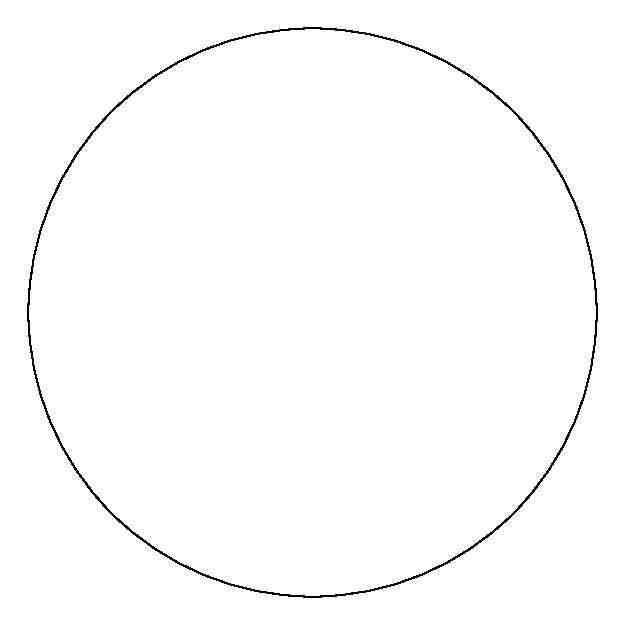
\includegraphics[height=4cm]{arc-length/pictures/09-01-circlea.pdf}%
%}%
%\only<handout:0| 3>{%
%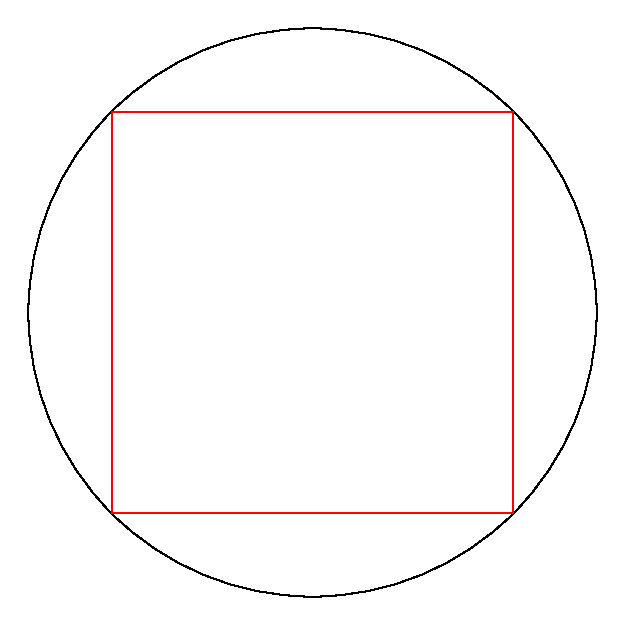
\includegraphics[height=4cm]{arc-length/pictures/09-01-circleb.pdf}%
%}%
%\only<handout:0| 4>{%
%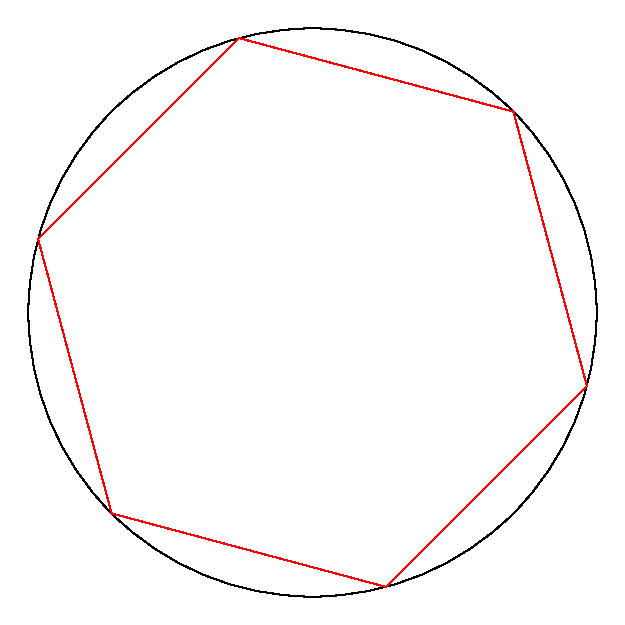
\includegraphics[height=4cm]{arc-length/pictures/09-01-circlec.pdf}%
%}%
%\only<handout:0| 5>{%
%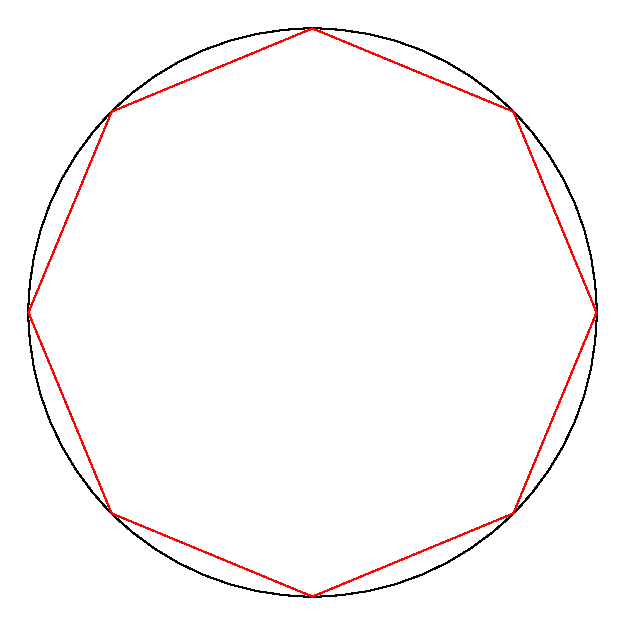
\includegraphics[height=4cm]{arc-length/pictures/09-01-circled.pdf}%
%}%
%\only<handout:0| 6>{%
%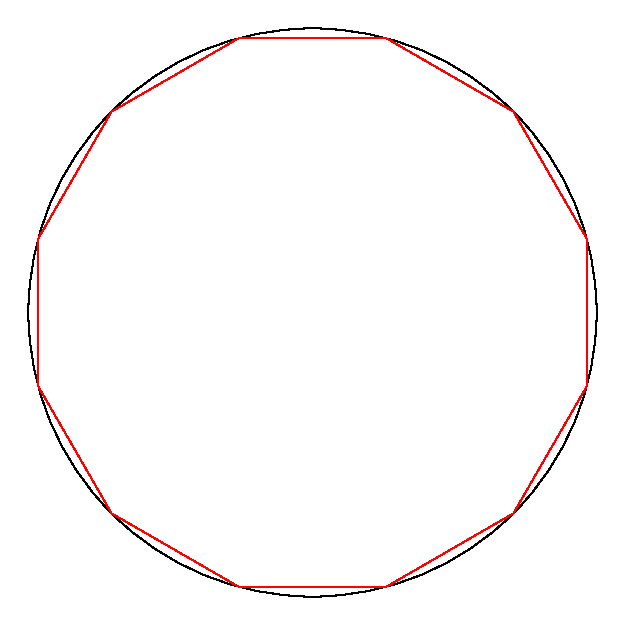
\includegraphics[height=4cm]{arc-length/pictures/09-01-circlee.pdf}%
%}%
%\only<handout:0| 7->{%
%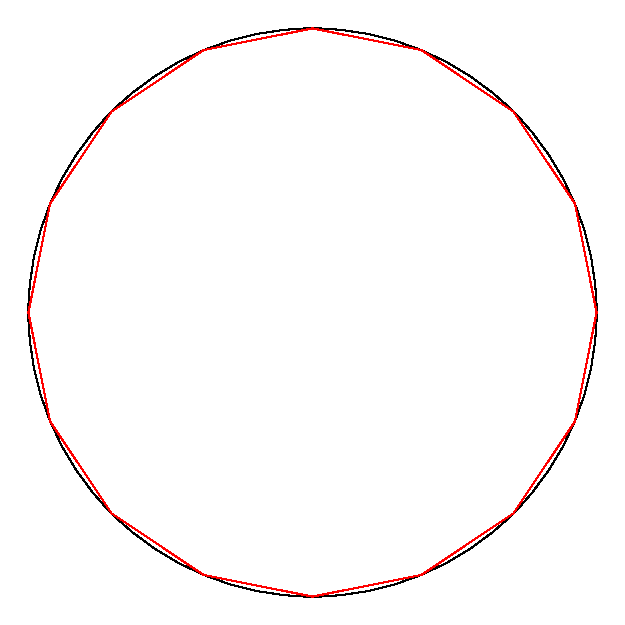
\includegraphics[height=4cm]{arc-length/pictures/09-01-circlef.pdf}%
%}%
\end{center}
\begin{itemize}
\item  What do we mean by the length of a curve?
\item<2->  The length of a polygon is easy to compute: add up the length of the line segments that form the polygon.
\item<3->  If the curve is a circle, approximate it by a polygon.
\item<4->  Then take the limit as the number of segments of the polygon goes to $\infty$.
\end{itemize}
\end{frame}
% end module arc-length-intro

%%begin module arc-length-derivation-parametric
{% scoping block for the following command:
%Calculator input: plotCurve{}(t, 8 t^{4}-40 t^{3}+70 t^{2}-50 t+13, 2/5, 2)
\newcommand{\theCurve}{t 13 t -50 mul add t 2 exp 70 mul add t 3 exp -40 mul add t 4 exp 8 mul add}
\newcommand{\lowBound}{0.4}
\newcommand{\highBound}{2}
\begin{frame}
Let $\gamma $ be the curve
$ \gamma: \left|
\begin{array}{rcl}
x=x(t)\\
y=y(t)
\end{array}, t\in [a,b]
\right.$

\begin{itemize}
\item<2->  Divide $[a,b]$ into $n$ subintervals with endpoints $t_0, t_1, \ldots , t_n$ and equal width $\Delta t$.
\item<3->  The points $P_i = (x(t_i), y(t_i))$ lie on the curve $\gamma$. The lengths of the segments with endpoints with consecutive indices from $P_0, P_1, \ldots , P_n$ approximate the length of the curve $\gamma$.
\item<4->  The length $L$ of the curve $\gamma$ is the limit of the lengths of these segments as $n\rightarrow \infty$.
\end{itemize}
\begin{columns}[c]
\column{.6\textwidth}
\begin{center}
\psset{xunit=1.4cm, yunit=1.4cm}
\begin{pspicture}(-0.4,-0.3)(2.3,1.994800)
\tiny
\fcAxesStandard{-0.3}{-0.3}{2.146803}{1.994800}
%\theCurve is defined in the beginning of this module, has limited scope
\parametricplot{\lowBound}{\highBound}{\theCurve}
\uncover<2-4>{%
\fcPolylineAlongCurveWithLabels[linecolor=\fcColorGraph]{3}{\lowBound}{\highBound}{\theCurve}{P}%
}
\uncover<5>{%
\fcPolylineAlongCurveWithLabels[linecolor=\fcColorGraph]{4}{\lowBound}{\highBound}{\theCurve}{P}%
}
\uncover<6>{%
\fcPolylineAlongCurveWithLabels[linecolor=\fcColorGraph]{5}{\lowBound}{\highBound}{\theCurve}{P}%
}
\uncover<6>{%
\fcPolylineAlongCurveWithLabels[linecolor=\fcColorGraph]{6}{\lowBound}{\highBound}{\theCurve}{P}%
}
\uncover<7>{%
\fcPolylineAlongCurveWithLabels[linecolor=\fcColorGraph]{10}{\lowBound}{\highBound}{\theCurve}{P}%
}
\uncover<8->{%0
\fcPolylineAlongCurveWithLabels[linecolor=\fcColorGraph]{14}{\lowBound}{\highBound}{\theCurve}{P}%
}
\end{pspicture}
%\ \only<handout:0| -1>{%
%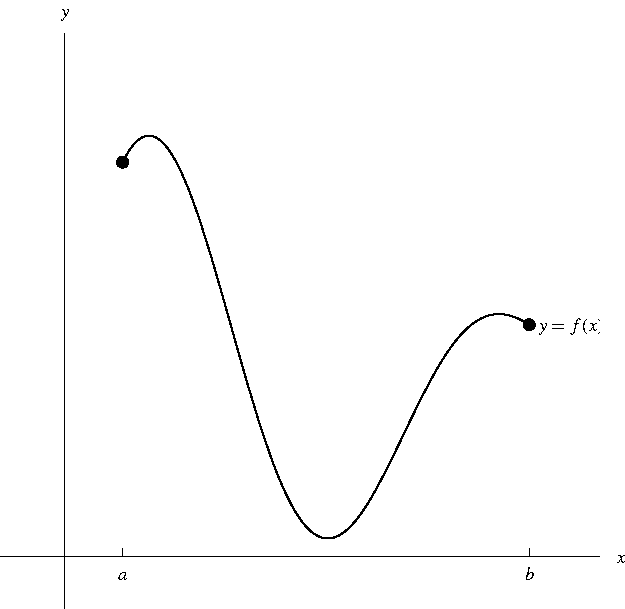
\includegraphics[height=4.5cm]{arc-length/pictures/09-01-arclengtha.pdf}%
%}%
%\only<handout:0| 2-4>{%
%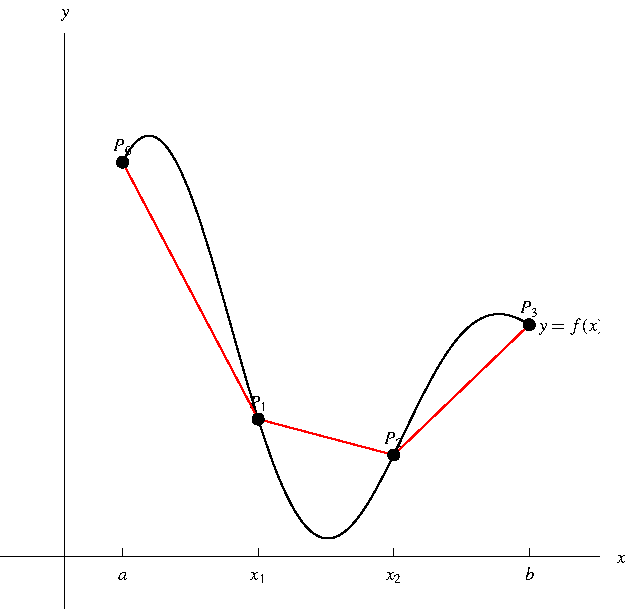
\includegraphics[height=4.5cm]{arc-length/pictures/09-01-arclengthb.pdf}%
%}%
%\only<handout:0| 5>{%
%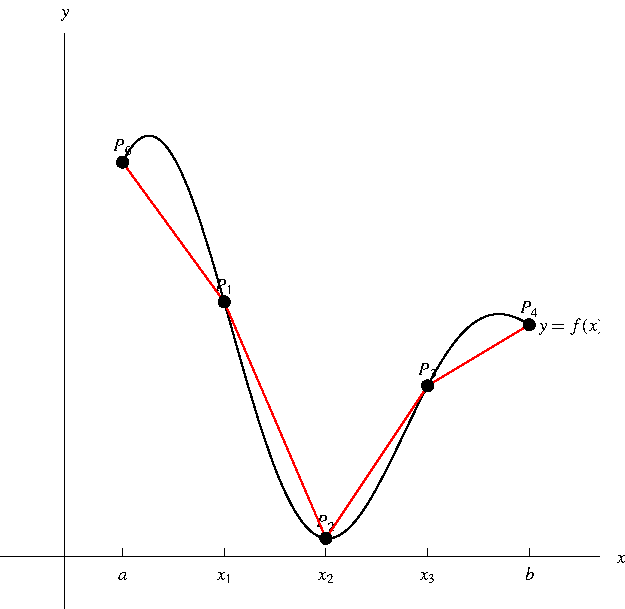
\includegraphics[height=4.5cm]{arc-length/pictures/09-01-arclengthc.pdf}%
%}%
%\only<handout:0| 6>{%
%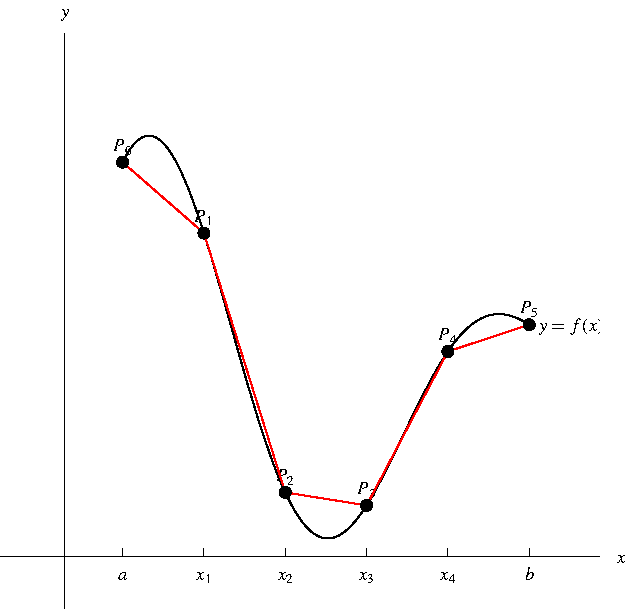
\includegraphics[height=4.5cm]{arc-length/pictures/09-01-arclengthd.pdf}%
%}%
%\only<handout:0| 7>{%
%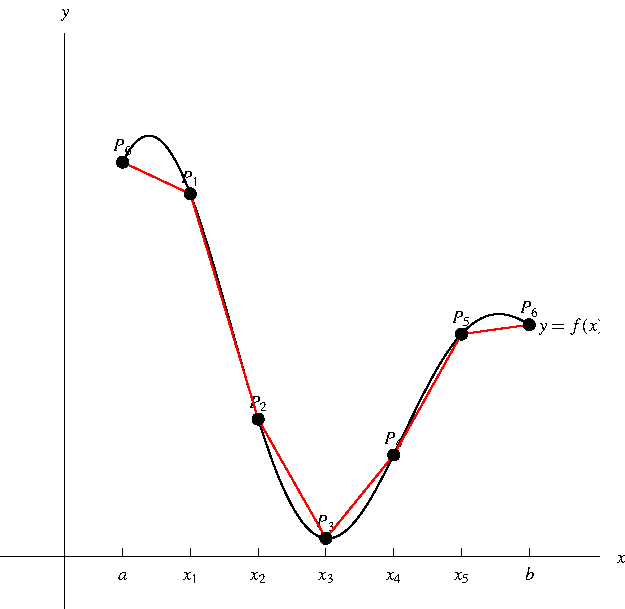
\includegraphics[height=4.5cm]{arc-length/pictures/09-01-arclengthe.pdf}%
%}%
%\only<8>{%
%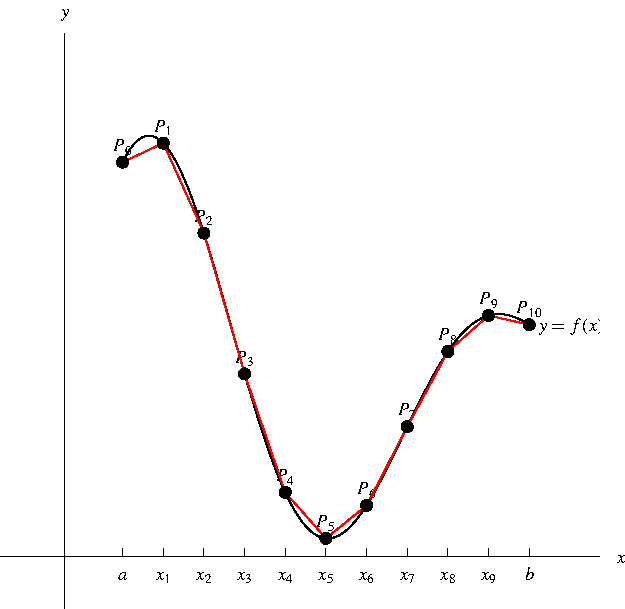
\includegraphics[height=4.5cm]{arc-length/pictures/09-01-arclengthf.pdf}%
%}%
%\only<handout:0| 9->{%
%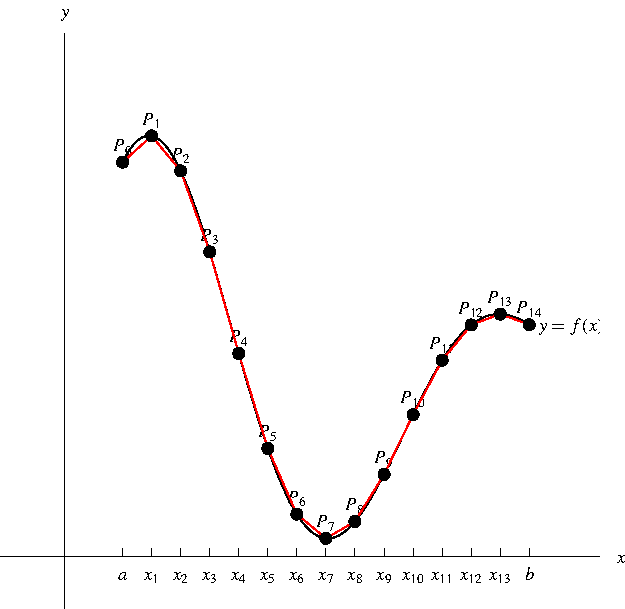
\includegraphics[height=4.5cm]{arc-length/pictures/09-01-arclengthg.pdf}%
%}%
%\only<10->{%
%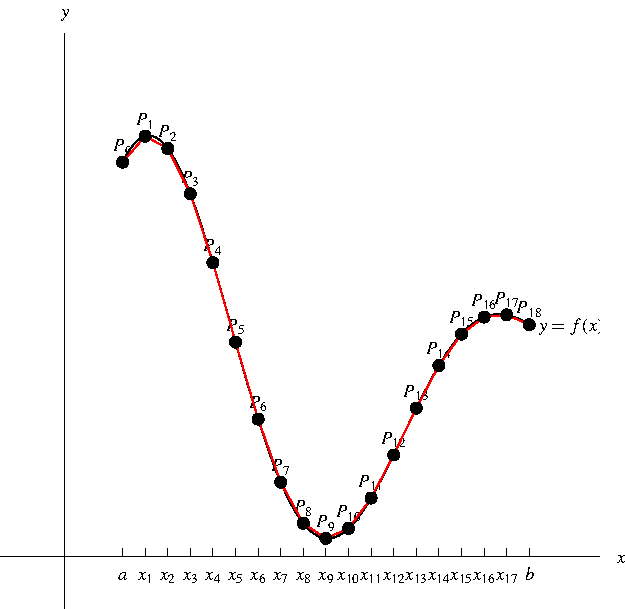
\includegraphics[height=4.5cm]{arc-length/pictures/09-01-arclengthh.pdf}%
%}%
\end{center}
\column{.4\textwidth}
\uncover<10->{%
\[
L = \lim_{n\rightarrow \infty} \sum_{i=1}^n |P_{i-1}P_i|
\]
}%
\end{columns}
\end{frame}



\begin{frame}
Let $\gamma $ be the curve
$ \gamma: \left|
\begin{array}{rcl}
x=x(t)\\
y=y(t)
\end{array}, t\in [a,b]
\right.$

$\begin{array}{rcl}
\uncover<1->{%
L = \lim_{n\rightarrow \infty} \sum_{i = 1}^n \alert<handout:0| 10>{|P_{i-1}P_i|}%
}%
& \uncover<10->{ = } &%
\uncover<10->{%
\alert<handout:0| 12>{\lim_{n\rightarrow\infty} \sum_{i=1}^n} \alert<handout:0| 10>{\sqrt{\alert<handout:0|13>{ (x'(s_i))^2}+\alert<handout:0| 13>{(y'(r_i))^2}}\ \alert<handout:0| 14>{\Delta t}}%
}\\%
& \uncover<11->{ = } &%
\uncover<11->{%
\alert<handout:0| 12>{\int_a^b} \sqrt{ \alert<handout:0| 13>{(x'(t))^2} +\alert<handout:0| 13>{(y'(t))^2}} \ \alert<handout:0| 14>{\diff t}%
}%
\end{array}
$
\begin{itemize}
\item  When $f$ has a continuous derivative we can compute arc length directly using the above limit.
\item<2->  Let $y_i = y(t_i)$, and $\Delta y = y_i - y_{i-1} = y(t_i) - y(t_{i-1})$.
\item<3-| alert@6>  Then $|P_iP_{i-1}| = \sqrt{(x(t_i)-x(t_{i-1}))^2+(y(t_i) -y(t_{i-1}))^2} = \sqrt{(\Delta x)^2 + (\Delta y)^2}$.
\item<4->  Mean Value Theorem: there exist numbers $s_i$ and $r_i$ between $t_{i-1}$ and $t_i$ such that $\alert<handout:0| 5>{x(t_i) - x(t_{i-1}) = x'(s_i )(t_i- t_{i-1})}$  and $\alert<handout:0| 5>{y(t_i) - y(t_{i-1}) = y'(r_i)( t_i-t_{i-1})}$
\item<5-| alert@5,7> $\Delta x = x'(s_i)\Delta t$, $\Delta y = y'(r_i)\Delta t$.
\end{itemize}
$\begin{array}{rcl}
\uncover<6->{%
\alert<handout:0| 10>{|P_{i-1}P_i|}%
}%
& \uncover<6->{\alert<handout:0| 10>{ = }} &%
\uncover<6->{%
\sqrt{(\alert<handout:0| 7>{\Delta x})^2 + (\alert<handout:0| 7>{\Delta y})^2}%
}  \uncover<7->{ = } \uncover<7->{%
\sqrt{ (\alert<handout:0| 7>{x'(s_i)\Delta t})^2 + (\alert<handout:0| 7>{y'(r_i)\Delta t})^2}%
}\\%
& \uncover<8->{ = } &%
\uncover<8->{%
\sqrt{(x'(s_i))^2 + (y'(r_i))^2}\sqrt{(\Delta t)^2}%
}  \uncover<9->{ = } \uncover<9->{%
\alert<handout:0| 10>{\sqrt{(x'(s_i))^2 + (y'(r_i))^2}\ \Delta t }%
}\\%
\end{array}
$
\end{frame}
}% end of scoping block
%end module arc-length-derivation-parametric

%% begin module arc-length-ex1
\begin{frame}
\begin{example}[Example 1, p. 562]
Find the length of the arc of $y^2 = x^3$ between $(1,1)$ and $(4,8)$.
\begin{columns}[c]
\column{.3\textwidth}
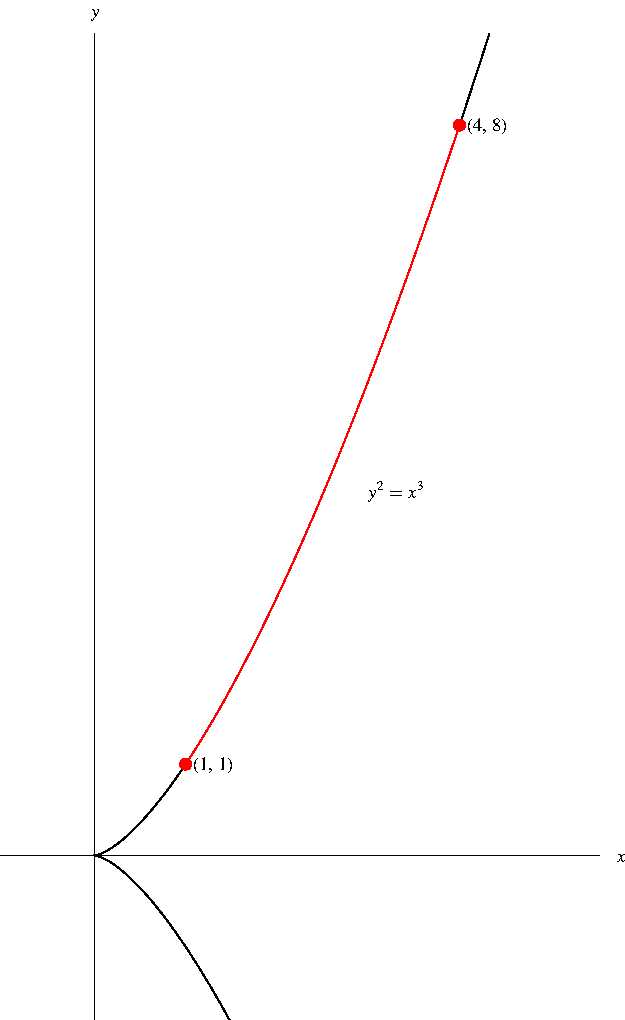
\includegraphics[height=6cm]{arc-length/pictures/09-01-ex1.pdf}%
\column{.7\textwidth}
\begin{itemize}
\item<2->  For the top half of the curve we have:
\item<2->  \alert<handout:0| 3-4>{$y = \uncover<4->{x^{3/2}}$} and  \alert<handout:0| 5-6,8>{$y' = \uncover<6->{\frac{3}{2}x^{1/2}}$}.
\item<9->  \alert<handout:0| 10-11>{$u = \uncover<11->{1 + \frac{9}{4}x}$} and  \alert<handout:0| 12-13>{$\diff u = \uncover<13->{\frac{9}{4}\diff x}$}.
\item<9-| alert@14-15>  When $x = 1$, $u = \uncover<15->{\frac{13}{4}}$.
\item<9-| alert@16-17>  When $x = 4$, $u = \uncover<17->{10}$.
\end{itemize}
\begin{eqnarray*}
\uncover<7->{%
L % 
}%
& \uncover<7->{ = } &%
\uncover<7->{%
\int_1^4 \sqrt{1+\left( \alert<handout:0| 8>{y'} \right)^2}\diff x%
}\\%
& \uncover<8->{ = } &%
\uncover<8->{%
\int_{\alert<handout:0| 14-15>{1}}^{\alert<handout:0| 16-17>{4}} \sqrt{\alert<handout:0| 11>{1+} \alert<handout:0| 8,11>{\frac{9}{4}x} }\ \alert<handout:0| 12-13>{\diff x}%
} \uncover<9->{ = } \uncover<9->{%
\int_{\alert<handout:0| 14-15>{\uncover<15->{13/4}}}^{\alert<handout:0| 16-17>{\uncover<17->{10}}} \alert<handout:0| 12-13>{\uncover<13->{\frac{4}{9}}}\uncover<11->{\sqrt{\alert<handout:0| 10-11>{u}}}\ \alert<handout:0| 12-13>{\uncover<13->{\diff u}}%
}\\%
& \uncover<18->{ = } &%
\uncover<18->{%
\frac{4}{9}\left[ \frac{2}{3} u^{3/2}\right]_{13/4}^{10}%
} \uncover<19->{ = } \uncover<19->{%
\frac{8}{27}\left( 10^{3/2} - \left( \frac{13}{4}\right)^{3/2}\right)%
}\\%
\end{eqnarray*}
\end{columns}
\end{example}
\end{frame}
% end module arc-length-ex1

%% begin module arc-length-half-ex
\begin{frame}
\begin{example}[$(a+b)^2$, $(a-b)^2$, $2ab=1/2$]
Find the length of the arc of $x = \frac{1}{6}e^{3x} + \frac{1}{6}e^{-3x}$ from $x = 0$ to $x = 1$.
\abovedisplayskip=0pt
\belowdisplayskip=0pt
\begin{eqnarray*}
\uncover<2->{\alert<handout:0| 2-3>{y'}} %
& \uncover<2->{\alert<handout:0| 2-3>{=}} & %
\uncover<3->{\alert<handout:0| 3>{\frac{1}{2}e^{3x} - \frac{1}{2}e^{-3x}}} \\%
\uncover<4->{\alert<handout:0| 8>{(y')^2}} %
& \uncover<4->{=} & %
\uncover<4->{\frac{1}{4}e^{6x} \alert<handout:0| 5-6>{- \frac{1}{4}e^{3x}e^{-3x} - \frac{1}{4}e^{3x}e^{-3x}} + \frac{1}{4}e^{-6x}} \\%
& \uncover<6->{\alert<handout:0| 8>{=}} & %
\uncover<6->{\alert<handout:0| 8>{\frac{1}{4}e^{6x} \alert<handout:0| 6>{- \frac{1}{2}} + \frac{1}{4}e^{-6x}}} \\%
\uncover<7->{L} %
& \uncover<7->{=} & %
\uncover<7->{\int_0^1 \sqrt{1 + \alert<handout:0| 8>{(y')^2}} \diff x} %
 \uncover<8->{=}  %
\uncover<8->{\int_0^1 \sqrt{\alert<handout:0| 9>{1} + \alert<handout:0| 8>{\frac{1}{4}e^{6x} \alert<handout:0| 9>{- \frac{1}{2}} + \frac{1}{4}e^{-6x}}} \diff x} \\%
& \uncover<9->{=} & %
\uncover<9->{\int_0^1 \sqrt{\frac{1}{4}e^{6x} \alert<handout:0| 9>{+ \frac{1}{2}} + \frac{1}{4}e^{-6x}} \diff x} %
 \uncover<10->{=}  %
\uncover<10->{\int_0^1 \sqrt{\left( \frac{1}{2}e^{3x} + \frac{1}{2}e^{-3x}\right)^2} \diff x} \\%
& \uncover<11->{=} & %
\uncover<11->{\int_0^1 \left( \alert<handout:0| 12-13>{\frac{1}{2}e^{3x}} + \alert<handout:0| 14-15>{\frac{1}{2}e^{-3x}}\right) \diff x} %
 \uncover<12->{=}  %
\uncover<12->{\left[ \uncover<13->{\alert<handout:0| 13>{\frac{1}{6}e^{3x}}} \uncover<15->{\alert<handout:0| 15>{- \frac{1}{6}e^{-3x}}}\right]_0^1} %
 \uncover<16->{=}  %
\uncover<16->{\frac{ e^3 - e^{-3}}{6}} %
\end{eqnarray*}
\end{example}
\end{frame}
% end module arc-length-half-ex

%% begin module cycloid-arc-length-ex5
\begin{frame}
\begin{example} %[Example 5, p. 671]
\begin{columns}[c]
\column{.4\textwidth}
\psset{xunit=0.6cm, yunit=0.6cm}
\begin{pspicture}(-0.9, -0.9)(6.8,2.6)
\tiny
\fcAxesStandard{-0.8}{-0.65}{6.8}{2.4}
\fcYTickWithLabel{2}{$2\pi r$}
\fcXTickWithLabel{6.28319}{$2\pi r$}
%Calculator input: plotCurve{}(- \sin{}t+t, - \cos{}t+1, 0, 2 \pi)
\parametricplot[linecolor=\fcColorGraph, plotpoints=1000]{0}{6.28319}{t t 57.29578 mul sin -1 mul add 1 t 57.29578 mul cos -1 mul add }
\end{pspicture}
%\ 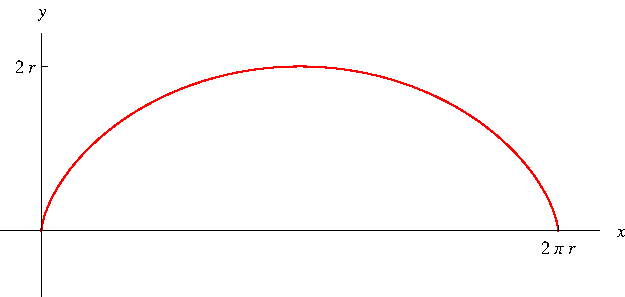
\includegraphics[height=2.2cm]{parametric-curves/pictures/11-02-ex5.pdf}%
\column{.6\textwidth}
Find the length of one arch of the cycloid
\[
\alert<handout:0| 3-4>{x = r(\theta - \sin \theta )}, \quad  \alert<handout:0| 5-6>{y = r(1-\cos \theta )}.%
\]
\uncover<2->{%
The first arch is \alert<handout:0| 2,12>{$0\leq \theta \leq 2\pi$}.
}%
\end{columns}
\abovedisplayskip=0pt
\belowdisplayskip=0pt
\[
\uncover<2->{%
L = \int_{\alert<handout:0| 2>{0}}^{\alert<handout:0| 2>{2\pi}}\sqrt{\left( \alert<handout:0| 3-4>{\frac{\diff x}{\diff \theta}}\right)^2+\left( \alert<handout:0| 5-6>{\frac{\diff y}{\diff \theta}}\right)^2} \diff \theta%
}%
\uncover<3->{%
 = \int_0^{2\pi}\sqrt{\left( \alert<handout:0| 3-4>{\uncover<4->{r(1-\cos \theta )}}\right)^2+\left( \alert<handout:0| 5-6>{\uncover<6->{r\sin \theta}}\right)^2} \diff \theta%
}%
\]
\abovedisplayskip=0pt
\belowdisplayskip=0pt
\[
\uncover<7->{%
 = \int_0^{2\pi} \sqrt{r^2(1 - 2\cos \theta + \cos^2\theta + \sin^2\theta)}\diff \theta%
}%
\uncover<8->{%
 = r \int_0^{2\pi} \sqrt{2(1 - \cos \theta)}\diff \theta%
}%
\]
\uncover<9->{%
Use the identity \alert<handout:0| 10>{$\sin^2 x = \frac{1}{2}(1-\cos 2x)$}.  %
}%
\uncover<10->{%
Then %
}%
\abovedisplayskip=0pt
\belowdisplayskip=0pt
\[
\uncover<9->{%
\sqrt{\alert<handout:0| 10>{2(1-\cos \theta )}}%
}%
\uncover<10->{%
 = \sqrt{\alert<handout:0| 10>{4\sin^2 (\theta /2) }}%
}%
\uncover<11->{%
 = 2\alert<handout:0| 12>{|}\sin (\theta /2)\alert<handout:0| 12>{|}%
}%
\uncover<12->{%
 = 2\sin (\theta /2)%
}%
\]
\abovedisplayskip=0pt
\belowdisplayskip=0pt
\[
\uncover<13->{%
L = r\int_0^{2\pi}2\sin (\theta /2)\diff \theta%
}%
\uncover<14->{%
 = r\left[ -4\cos (\theta / 2)\right]_0^{2\pi}%
}%
%\uncover<15->{%
% = r\left( (-4)(-1) - (-4)(1)\right)%
%}%
\uncover<15->{%
 = 8r%
}%
\]
\end{example}
\end{frame}
% end module cycloid-arc-length-ex5

%% begin module cardioid-arc-length-ex4
\begin{frame}[t]
\begin{example} %[Example 4, p. 688]
\begin{columns} 
\column{0.2\textwidth}
\psset{xunit=0.5cm, yunit=0.5cm}
\begin{pspicture}(-1.699025, -0.9)(1.699025,2.499985) 
\tiny 
\psaxesStandard{-1.449025}{-0.65}{1.449025}{2.149985}
%Calculator command: drawPolar{}(\sin{}t+1, 0, 2 \pi) 
\parametricplot[linecolor=\psColorGraph, plotpoints=1000, algebraic=false]{0}{6.28319}{ 1 t 57.29578 mul sin add t 57.29578 mul cos mul 1 t 57.29578 mul sin add t 57.29578 mul sin mul }
\end{pspicture} 
\column{0.8\textwidth}
Find the length of the cardioid \alert<handout:0| 3-6>{$r = 1 + \sin \theta$}.
\uncover<2->{%
The full length is given by \alert<handout:0| 2>{$0\leq \theta \leq 2\pi$}.
}%
\end{columns}
\abovedisplayskip=0pt
\belowdisplayskip=0pt
%\begin{eqnarray*}
\[
\begin{array}{l}
\uncover<2->{%
\displaystyle L  = \displaystyle  \int_{\alert<handout:0| 2>{0}}^{\alert<handout:0| 2>{2\pi}} \sqrt{\alert<handout:0| 3-4>{r^2} + \alert<handout:0| 5-6>{\left( \frac{\diff r}{\diff \theta}\right)^2}}\diff \theta%
}%
\uncover<3->{%
\displaystyle  = \int_0^{2\pi} \sqrt{\alert<handout:0| 4>{\uncover<4->{(1+\sin \theta )^2}} + \alert<handout:0| 6>{\uncover<6->{\cos^2\theta}}}\diff \theta%
}\\%
 \uncover<7->{ = } %
\uncover<7->{%
\displaystyle \int_0^{2\pi} \sqrt{2 + 2\sin\theta}\only<8->{\alert<handout:0| 8>{\frac{\sqrt{2-2\sin\theta}}{\sqrt{2-2\sin\theta}}}}\diff \theta%
}%
\uncover<9->{%
\displaystyle  = \int_0^{2\pi} \frac{\sqrt{4 - 4\sin^2\theta}}{\sqrt{2-2\sin\theta}}\diff \theta%
}\\%
 \uncover<10->{ = } %
\uncover<10->{%
\displaystyle \int_0^{2\pi} \frac{\alert<handout:0| 11>{\sqrt{4\cos^2\theta}}}{\sqrt{2-2\sin\theta}}\diff \theta%
}%
\uncover<11->{%
\displaystyle  = \int_{\alert<handout:0| 12>{0}}^{\alert<handout:0| 12>{2\pi}} \frac{\alert<handout:0| 11-12>{2|\cos\theta |}}{\sqrt{2-2\sin\theta}}\diff \theta%
}\\%
 \uncover<12->{ = } %
\uncover<12->{%
\displaystyle \int_{\alert<handout:0| 12>{0}}^{\alert<handout:0| 12>{\pi/2}}\frac{\alert<handout:0| 12>{2\cos \theta}}{\sqrt{2-2\sin\theta}}\diff\theta%
 + \int_{\alert<handout:0| 12>{\pi/2}}^{\alert<handout:0| 12>{3\pi /2}}\frac{\alert<handout:0| 12>{-2\cos \theta}}{\sqrt{2-2\sin\theta}}\diff\theta%
 + \int_{\alert<handout:0| 12>{3\pi/2}}^{\alert<handout:0| 12>{2\pi}}\frac{\alert<handout:0| 12>{2\cos \theta}}{\sqrt{2-2\sin\theta}}\diff\theta%
}\\%
 \uncover<13->{ = } %
\uncover<13->{%
\displaystyle \left[ -2\alert<handout:0| 14-17>{\sqrt{2-2\sin\theta}}\right]_{\alert<handout:0| 16-17>{0}}^{\alert<handout:0| 14-15>{\pi/2}}%
\displaystyle  + \left[ 2\alert<handout:0| 18-21>{\sqrt{2-2\sin\theta}}\right]_{\alert<handout:0| 20-21>{\pi/2}}^{\alert<handout:0| 18-19>{3\pi/2}}%
\displaystyle  + \left[ -2\alert<handout:0| 22-25>{\sqrt{2-2\sin\theta}}\right]_{\alert<handout:0| 24-25>{3\pi/2}}^{\alert<handout:0| 22-23>{2\pi}}%
}\\%
 \uncover<14->{ = } %
\uncover<14->{%
\displaystyle -2\left( \uncover<15->{\alert<handout:0| 15>{0}} - \uncover<17->{\alert<handout:0| 17>{\sqrt{2}}}\right)%
\displaystyle +2\left( \uncover<19->{\alert<handout:0| 19>{2}} - \uncover<21->{\alert<handout:0| 21>{0}}\right)%
\displaystyle -2\left( \uncover<23->{\alert<handout:0| 23>{\sqrt{2}}} - \uncover<25->{\alert<handout:0| 25>{2}}\right)%
}%
 \uncover<26->{ = } %
\uncover<26->{%
8%
}%
%\end{eqnarray*}
\end{array}
\]
\end{example}
\end{frame}
% end module cardioid-arc-length-ex4

%% begin module arcsin-def
\begin{frame}
\frametitle{Inverse Trigonometric Functions}
\psset{xunit=0.6cm,yunit=0.6cm}
\begin{pspicture}(-5,-1.4)(10,1.4)
\tiny
\psaxes[labels=none, Dx=1.570796327, Dy=1] {<->}(0,0)(-4,-1.8)(10,1.8)

\uncover<1-2| handout:0>{\psplot[linecolor=red, plotpoints=1000]{-4}{10}{x 57.295779513 mul sin}}
\uncover<2| handout:0>{\psline(-4,0.6)(10,0.6 )}

\uncover<3>{\psplot[linecolor=red, plotpoints=1000]{-1.570796327}{1.570796327}{x 57.295779513 mul sin}
\rput[bl](3, 1){\alert<3>{$y=\sin x, -\frac{\pi}{2}\leq x\leq \frac{\pi}{2}$} }
}
\uncover<4-| handout:0>{\psplot[linecolor=gray, plotpoints=1000]{-1.570796327}{1.570796327}{x 57.295779513 mul sin}
\rput[bl](3, 1){\color{gray}{$y=\sin x, -\frac{\pi}{2}\leq x\leq \frac{\pi}{2}$} }
}

\uncover<4-| handout:0>{\psplot[linecolor=red, plotpoints=1000]{-1}{1}{x ASIN}
\rput[r](-1.5, -1){\alert<4>{$y=\Arcsin x$} }

}

\rput[t](-3.14, -0.3){$-\pi$}
\rput[t](-1.57, -0.3){$-\frac{\pi}{2}$}
\rput[t](1.57, -0.3){$\frac{\pi}{2}$}
\rput[t](3.14, -0.3){$\pi$}
\rput[t](4.71, -0.3){$\frac{3\pi}{2}$}
\rput[t](6.28, -0.3){$2\pi$}
\rput[t](7.85, -0.3){$\frac{5\pi}{2}$}
\rput[t](9.42, -0.3){$3\pi$}
\rput[bl](0.2,1){\tiny $1$}
\end{pspicture}
\begin{columns}[c]
\column{.65\textwidth}
\begin{itemize}
\item<2->  $\sin x$ isn't one-to-one.
\item<3->  It is if we restrict the domain to $\left[-\frac{\pi}{2}, \frac{\pi}{2}\right]$.
\item<4->  Then it has an inverse function.
\item<4->  We call it $\arcsin$ or $\sin^{-1}$.
\item<6->  $\Arcsin x = y \Leftrightarrow \sin y = x$ and $-\frac{\pi} {2} \leq y \leq \frac{\pi}{2}$.
\end{itemize}
\column{.35\textwidth}
\psset{xunit=1cm,yunit=1cm}
\uncover<5->{
\begin{pspicture}(-1.5,-2)(1.7,2)
\tiny
\psaxes[ticks=none, labels=none]{<->}(0,0)(-1.5,-2)(1.5,2)
\fcLabels{1.5}{2}
\fcLabelXOne
\psline(-1, -0.1)(-1,0.1)
\rput[t](-1,  -0.1){$-1$}

\psline(-0.1, 1.570796327)(0.1,1.570796327)
\rput[r](-0.1,  1.570796327){$\frac{\pi}{2}$}
\psline(-0.1, -1.570796327)(0.1,-1.570796327)
\rput[r](-0.1,  -1.570796327){$-\frac{\pi}{2}$}

\psplot[linecolor=red, plotpoints=1000]{-1}{1}{x ASIN}
\rput[rb](-0.05, 0.2){\alert<4>{$y=\Arcsin x$} }
\fcFullDot{1}{1.570796327}
\fcFullDot{-1}{-1.570796327}
\end{pspicture}
}
%\uncover<5->{%
%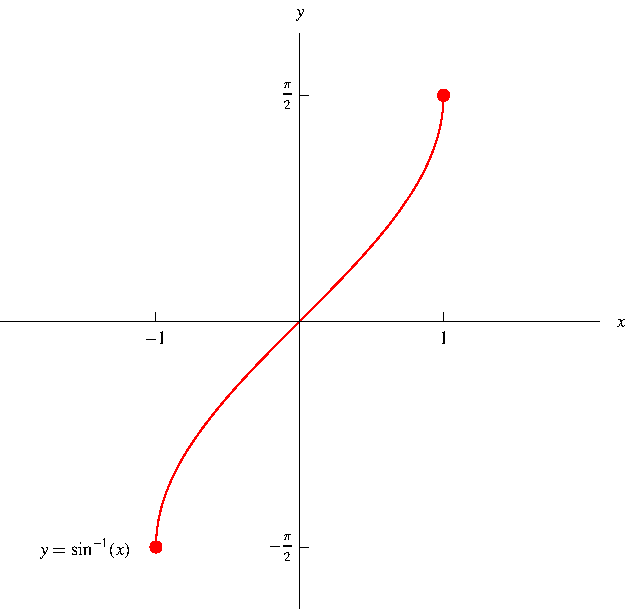
\includegraphics[height=4cm]{inverse-trig/pictures/07-06-arcsine.pdf}%
%}%

\end{columns}
\end{frame}
% end module arcsin-def

%% begin module arcsin-properties
\begin{frame}
Important facts about $\Arcsin$:
\begin{columns}[c]
\column{.5\textwidth}
%\ 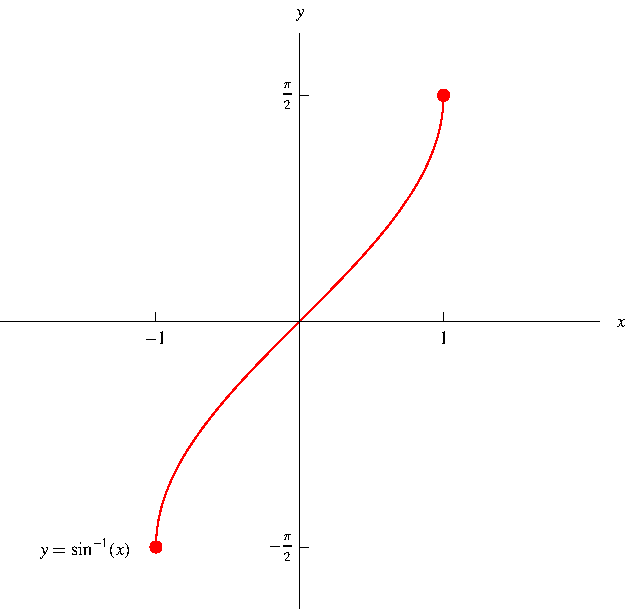
\includegraphics[height=6cm]{inverse-trig/pictures/07-06-arcsine.pdf}%
\psset{xunit=2cm,yunit=2cm}
\begin{pspicture}(-5,-1.4)(10,1.4)
\tiny
\psaxes[ticks=none, labels=none]{<->}(0,0)(-1.5,-2)(1.5,2)
\psLabels{1.5}{2}
\psLabelXOne
\psline(-1, -0.1)(-1,0.1)
\rput[t](-1,  -0.1){$-1$}

\psline(-0.1, 1.570796327)(0.1,1.570796327)
\rput[r](-0.1,  1.570796327){$\frac{\pi}{2}$}
\psline(-0.1, -1.570796327)(0.1,-1.570796327)
\rput[r](-0.1,  -1.570796327){$-\frac{\pi}{2}$}

\psplot[linecolor=red, plotpoints=1000]{-1}{1}{x ASIN}
\rput[rb](-0.05, 0.2){$y=\Arcsin x$} 
\psFullDot{1}{1.570796327}
\psFullDot{-1}{-1.570796327}
\uncover<3>{\psline[linecolor=red, linewidth=2pt]{<->}(-1,0)(1,0) }
\uncover<5>{\psline[linecolor=red, linewidth=2pt]{<->}(0,-1.570796327)(0,1.570796327) }

\end{pspicture}
\column{.5\textwidth}
\begin{enumerate}
\item  \alert<handout:0| 2-3>{Domain: \uncover<3->{$[-1, 1]$.}}
\item  \alert<handout:0| 4-5>{Range: \uncover<5->{$[-\pi /2, \pi /2]$.}}
\item  $\Arcsin x = y \Leftrightarrow \sin y = x$ and $-\pi /2 \leq y \leq \pi /2$.
\item  $\Arcsin (\sin x) = x$ for $-\pi /2 \leq x \leq \pi /2$.
\item  $\sin (\Arcsin x) = x$ for $-1 \leq x \leq 1$.
\item  $\frac{\diff}{\diff x} (\Arcsin x) = \frac{1}{\sqrt{1-x^2}}$.
\end{enumerate}
\end{columns}
\end{frame}
% end module arcsin-properties


%% begin module arccos-def
\begin{frame}
%\ \only<handout:0| -1>{%
%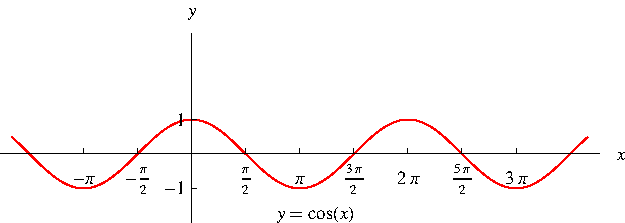
\includegraphics[width=12cm]{inverse-trig/pictures/07-06-arccosa.pdf}%
%}%
%\only<2>{%
%\includegraphics[width=12cm]{inverse-trig/pictures/07-06-arccosb.pdf}%
%}%
%\only<handout:0| 3->{%
%\includegraphics[width=12cm]{inverse-trig/pictures/07-06-arccosc.pdf}%
%}%
\psset{xunit=0.6cm,yunit=0.6cm}
\begin{pspicture}(-5,-1.4)(10,1.4)
\tiny
\psaxes[labels=none, ticks=x, Dx=1.570796327, Dy=1] {<->}(0,0)(-4.1,-1.4)(10,3.4)
\psLabels{10}{3.4}
\uncover<1>{\psplot[linecolor=red, plotpoints=1000]{-4}{10}{x 57.295779513 mul cos}
\rput[t](3.5, 1){$y=\cos x$}
}
\uncover<2>{\psplot[linecolor=red, plotpoints=1000]{0}{3.141592654}{x 57.295779513 mul cos}
\rput[t](3.5, 1){$y=\cos x, \quad 0\leq x\leq \pi$}
}
\uncover<3->{\psplot[linecolor=gray, plotpoints=1000]{0}{3.141592654}{x 57.295779513 mul cos}
\rput[t](3.5, 1){\color{gray}$y=\cos x, \quad 0\leq x\leq \pi$}

\psplot[linecolor=red, plotpoints=1000]{-1}{1}{x ACOS}
\psline(-0.1,3.141592654)(0.1,3.141592654)
\rput[l](0.15,3.141592654){$\pi$}
\psline(-1,-0.1)(-1,0.1)
\rput[t](-1,-0.1){$-1$}
\psline(1,-0.1)(1,0.1)
\rput[t](1,-0.1){$1$}
\rput[r](-0.6, 0.4){$y=\Arccos x$}
}

\rput[t](-3.14, -0.3){$-\pi$}
\rput[t](-1.57, -0.3){$-\frac{\pi}{2}$}
\rput[t](1.57, -0.3){$\frac{\pi}{2}$}
\rput[t](3.14, -0.3){$\pi$}
\rput[t](4.71, -0.3){$\frac{3\pi}{2}$}
\rput[t](6.28, -0.3){$2\pi$}
\rput[t](7.85, -0.3){$\frac{5\pi}{2}$}
\rput[t](9.42, -0.3){$3\pi$}
\rput[br](-0.2,1){\tiny $1$}

\end{pspicture}

\begin{columns}[c]
\column{.65\textwidth}
\begin{itemize}
\item<1->  Same for $\cos x$.
\item<2->  Restrict the domain to $[0, \pi ]$.
\item<3->  The inverse is called $\arccos$ or $\cos^{-1}$.
\item<5->  $\Arccos (x) = y \Leftrightarrow \cos y = x$ and $0 \leq y \leq \pi$.
\end{itemize}
\column{.35\textwidth}
\uncover<4->{%
%\uncover<4->{%
%\includegraphics[height=4cm]{inverse-trig/pictures/07-06-arccosd.pdf}%
%}%
\psset{xunit=1.2cm,yunit=1.2cm}
\begin{pspicture}(-5,-1.4)(10,1.4)
\tiny
\psaxes[labels=none, ticks=none] {<->}(0,0)(-2,-0.5)(1.6,3.7)
\psLabels{1.6}{3.7}
\psplot[linecolor=red, plotpoints=1000]{-1}{1}{x ACOS}
\psline(-0.1,3.141592654)(0.1,3.141592654)
\rput[l](0.15,3.141592654){$\pi$}
\psline(-1,-0.1)(-1,0.1)
\rput[t](-1,-0.1){$-1$}
\psline(1,-0.1)(1,0.1)
\rput[t](1,-0.1){$1$}
\rput[r](-0.6, 2){$y=\Arccos x$}
\end{pspicture}
}%
\end{columns}
\end{frame}
% end module arccos-def



%% begin module inverse-trig-summary
\begin{frame}[t]
The remaining inverse trigonometric functions aren't used as often:
\[
\begin{array}{llcrcl}
y = \Arccsc x &%
(|x| \geq 1) &%
\alert<0>{\Leftrightarrow}&%
\csc y = x &%
\text{ and } &%
y\in \left(0,\frac{\pi}{2}\right] \cup \left(\pi , \frac{3\pi}{2} \right] \\%
\alert<2>{y = \Arcsec x }&%
\alert<2>{(|x| \geq 1) }&%
\alert<2>{\Leftrightarrow}&%
\alert<2>{\sec y = x }&%
\alert<2>{\text{ and } }&%
\alert<2>{y\in  \left[0,\frac{\pi}{2}\right) \cup \left[\pi , \frac{3\pi}{2}\right) }\\%
y = \Arccot x &%
(|x| \in \mathbb{R}) &%
\alert<0>{\Leftrightarrow}&%
\cot y = x &%
\text{ and } &%
y\in (0,\pi )
\end{array}
\]
\end{frame}
\begin{frame}
We will however make use of $\Arcsec x$: we discuss in detail its domain. 
\[
\begin{array}{llcrcl}
\alert<1>{y = \Arcsec x }&%
\alert<1>{(|x| \geq 1) }&%
\alert<1>{\Leftrightarrow }&%
\alert<1>{\sec y = x }&%
\alert<1>{\text{ and } }&%
\alert<1>{y\in\only<1-6>{\alert<1-6>{\textbf{?}}} \uncover<7->{\alert<7>{ \left[0,\frac{\pi}{2}\right) \cup \left[\pi , \frac{3\pi}{2}\right) }}}
\end{array}
\]

\begin{columns}
\column{0.43\textwidth}
\psset{xunit=0.5cm, yunit=0.5cm}
\begin{pspicture}(-5.2, -5.2)(5.2,5.2) 
\tiny 
\psaxesStandard{-5.15}{-5.15}{5.15}{5.15}

\uncover<1-7>{
\psline[linestyle=dashed](-1.570796327,-5 )(-1.570796327,5)
\psline[linestyle=dashed](1.570796327,-5 )(1.570796327,5)
\psline[linestyle=dashed](4.71238898,-5 )(4.71238898,5)
}
\uncover<10->{
\psline[linestyle=dashed](-5,-1.570796327)(5,-1.570796327)
\psline[linestyle=dashed](-5,1.570796327)(5,1.570796327)
\psline[linestyle=dashed](-5,4.71238898)(5,4.71238898)
}

\psXTickWithLabel{-1.570796327}{$-\frac{\pi}{2}$}
\psXTickWithLabel{1}{$1$}
\psXTick{1.570796327}
\rput[tl](1.6,-0.1){$\frac{\pi}{2}$}
\psXTickWithLabel{3.141592654}{$\pi$}
\psXTick{4.71238898}
\rput[tr](4.65,-0.1){$\frac{3\pi}{2}$}
\psYTickWithLabel{1}{$1$}
\psYTickWithLabel{1.570796327}{$\frac{\pi}{2}$}
\psYTickWithLabel{3.141592654}{$\pi$}
\psYTickWithLabel{4.71238898}{$\frac{3\pi}{2}$}

\uncover<2->{
\rput[l](1.6,4.5){$y=\sec x$}
}
\uncover<9->{
\rput[br](4.9,1.5){$y=\Arcsec x$}
}
\uncover<2-3>{%
%Function formula: 1/\cos{}x 
\psplot[linecolor=\psColorGraph, plotpoints=1000]{-4.511031}{-1.772154}{x 57.29578 mul cos -1 exp }
}%
\uncover<4->{%
%Function formula: 1/\cos{}x 
\psplot[linecolor=gray!10, plotpoints=1000]{-4.511031}{-1.772154}{x 57.29578 mul cos -1 exp }
}%
\uncover<2-4,6>{%
%Function formula: 1/\cos{}x 
\psplot[linecolor=\psColorGraph, plotpoints=1000]{-1.369438}{0}{x 57.29578 mul cos -1 exp }
}%uncover
\uncover<5,7->{%
%Function formula: 1/\cos{}x 
\psplot[linecolor=gray!40, plotpoints=1000]{-1.369438}{0}{x 57.29578 mul cos -1 exp }
}%
\uncover<2->{%
%Function formula: 1/\cos{}x 
\psplot[linecolor=\psColorGraph, plotpoints=1000]{0}{1.369438}{x 57.29578 mul cos -1 exp }
}%
\uncover<2-3>{
%Function formula: 1/\cos{}x 
\psplot[linecolor=\psColorGraph, plotpoints=1000]{1.772154}{3.141592654}{x 57.29578 mul cos -1 exp }
}%
\uncover<4->{
%Function formula: 1/\cos{}x 
\psplot[linecolor=gray!40, plotpoints=1000]{1.772154}{3.141592654}{x 57.29578 mul cos -1 exp }
}%
\uncover<2-3,5,7->{
%Function formula: 1/\cos{}x 
\psplot[linecolor=\psColorGraph, plotpoints=1000]{3.141592654}{4.511031}{x 57.29578 mul cos -1 exp }
}%uncover
\uncover<4,6>{
%Function formula: 1/\cos{}x 
\psplot[linecolor=gray!40, plotpoints=1000]{3.141592654}{4.511031}{x 57.29578 mul cos -1 exp }
}%uncover
\uncover<8->{%
\psline[linestyle=dashed, linecolor=\psColorTangent](-4.9,-4.9)(4.9,4.9)
}
\uncover<9->{
%Function formula: - \arccos{}(x^{-1})+2 \pi 
\psplot[linecolor=\psColorGraph, plotpoints=1000]{-5}{-1.00001}{ 3.141592654 2 mul x -1 exp ACOS -1 mul add }
%Function formula: \arccos{}(x^{-1}) 
\psplot[linecolor=gray!40, plotpoints=1000]{-5}{-1.00001}{x -1 exp ACOS }
%Function formula: \arccos{}(x^{-1}) 
\psplot[linecolor=\psColorGraph, plotpoints=1000]{1.00001}{5}{x -1 exp ACOS }
%Function formula: -\arccos{}(x^{-1}) 
\psplot[linecolor=gray!40, plotpoints=1000]{1.00001}{5}{x -1 exp ACOS -1 mul}
}
\end{pspicture} 
%\ \only<handout:0| -1>{%
%\includegraphics[width=5cm]{inverse-trig/pictures/07-06-seca.pdf}%
%}%
%\only<2->{%
%\includegraphics[width=5cm]{inverse-trig/pictures/07-06-secb.pdf}%
%}%
\column{0.57\textwidth}
\begin{itemize} 
\item<2-> \noindent Plot $\sec x$. 
\item<3-> Restrict domain to make one-to-one: Two common choices: \alert<4>{$x\in \left(-\frac{\pi}{2}, \frac{\pi}{2} \right) $} and \alert<5>{$x\in \left(0, \frac{\pi}{2} \right) \cup \left(\pi,\frac{3\pi}{2} \right) $}. 

\item<6-> $x\in \left(-\frac{\pi}{2}, \frac{\pi}{2} \right) $ is good because the domain is a single interval. \textbf{NOT our choice.}

\item<7,8,9,10-> $x\in \left(0, \frac{\pi}{2} \right) \cup \left(\pi,\frac{3\pi}{2} \right) $ is  good because $\tan x$ is positive on both intervals, resulting in easier differentiation and integration formulas. \textbf{Our choice.} 

\end{itemize}
\end{columns}

\end{frame}

\begin{frame}
Table of derivatives of inverse trigonometric functions: 
\begin{align*}
\frac{\diff}{\diff x} (\Arcsin x) & = %
\frac{1}{\sqrt{1-x^2}} &%
\frac{\diff}{\diff x} (\Arccsc x) & = %
-\frac{1}{x\sqrt{x^2-1}} \\%
\frac{\diff}{\diff x} (\Arccos x) & = %
-\frac{1}{\sqrt{1-x^2}} &%
\frac{\diff}{\diff x} (\Arcsec x) & = %
\frac{1}{x\sqrt{x^2-1}} \\%
\frac{\diff}{\diff x} (\Arctan x) & = %
\frac{1}{1+x^2} &%
\frac{\diff}{\diff x} (\Arccot x) & = %
-\frac{1}{1+x^2} %
\end{align*}
\end{frame}
% end module inverse-trig-summary


%% begin module cycloid-equations-ex7
\begin{frame}
\begin{example} %[Example 7, p. 660]
Find parametric equations of a cycloid made using a circle with radius $r$ that rolls along the $x$-axis such that $P$ hits the origin.
\begin{columns}[c]
\column{.4\textwidth}

\psset{xunit=1.7cm, yunit=1.7cm}
\begin{pspicture}(-1.000000, -5)(1.500000,5) 
\psframe*[linecolor=white](-1.000000,-5)(5.500000,5) 
\tiny 
\psaxes[arrows=<->, ticks=none, labels=none ]( 0,0)( -0.500000, -0.5)(2.55,2.2)

%Function formula: - (- (x-1256637061/1000000000)^{2}+1 )^{1/2}+1 
\psplot[linecolor=\psColorTangent, plotpoints=1000] {0.256647} {2.256627}{1 1 -1.25664 x add 2 exp -1 mul add 0.5 exp -1 mul add }
%Function formula: (- (x-1256637061/1000000000)^{2}+1 )^{1/2}+1 
\psplot[linecolor=\psColorTangent, plotpoints=1000] {0.256647} {2.256627}{1 1 -1.25664 x add 2 exp -1 mul add 0.5 exp add }
\uncover<2->{
\psplot[linecolor=green, plotpoints=300]{0.305581} {1.256637061} {1 1 -1.25664 x add 2 exp -1 mul add 0.5 exp -1 mul add }
}

%Calculator input: plotCurve{}(- \sin{}t+t, - \cos{}t+1, 0, \pi)
\parametricplot[linecolor=\psColorGraph, plotpoints=1000] { 0}{2.8}{t t 57.29578 mul sin -1 mul add 1 t 57.29578 mul cos -1 mul add }

\psFullDot{0.305581}{0.690983}
\rput[r](0.2, 0.69){$P$}
\psFullDot{1.256637061}{1}
\rput[bl](1.286637061,1.05){\uncover<5->{\alert<5>{$ C=(r\theta,r)$}}}

\uncover<6->{\psline[linestyle=dashed](0.305581,0)(0.305581,0.690983)
\rput[b](0.15, 0.05){\alert<6>{$x$}}
\rput[l](0.32, 0.35){\alert<6>{$y$}}
}

\psline(0.305581,0.690983)(1.256637061,1)
\rput[b](0.75, 0.85){$r$}

\uncover<7->{
\psline[linestyle=dashed](0.305581,0.690983)(1.256637061,0.690983)
\psline(1.156637061,0.690983)(1.156637061,0.590983)(1.256637061,0.590983)
\rput[l](1.306637061,0.690983){$Q$}
}

\psline(1.256637061,0.1)(1.356637061,0.1)(1.356637061,0)
\rput[lt](1.256637061,-0.1){$T$}
\psline(1.256637061,1)(1.256637061,0)

\uncover<3->{\psline[linecolor=green](0,0)(1.256637061, 0)}

\uncover<4->{
\psline{<-}(0,-0.2)(0.5, -0.2)
\psline{->}(0.72,-0.2)(1.256637061, -0.2)
\rput(0.62, -0.2){\alert<4>{$r\theta$}}
}
\rput(1.2, 0.9){\uncover<2->{\alert<2>{$\theta$}}}
\rput (-0.2, -0.2){$O$}
\end{pspicture} 

%\ \only<handout:0| -2>{%
%\includegraphics[width=5cm]{parametric-curves/pictures/11-01-cycloideqa.pdf}%
%}%
%\only<handout:0| 3>{%
%\includegraphics[width=5cm]{parametric-curves/pictures/11-01-cycloideqb.pdf}%
%}%
%\only<handout:0| 4>{%
%\includegraphics[width=5cm]{parametric-curves/pictures/11-01-cycloideqc.pdf}%
%}%
%\only<handout:0| 5>{%
%\includegraphics[width=5cm]{parametric-curves/pictures/11-01-cycloideqd.pdf}%
%}%
%\only<handout:0| 6>{%
%\includegraphics[width=5cm]{parametric-curves/pictures/11-01-cycloideqe.pdf}%
%}%
%\only<7->{%
%\includegraphics[width=5cm]{parametric-curves/pictures/11-01-cycloideqf.pdf}%
%}%
\column{.6\textwidth}
\begin{itemize}
\item<2->  We choose our parameter to be \alert<2>{$\theta$}, the angle of rotation of the circle.
\item<3->  How far has the circle moved if it has rolled through $\theta$ radians?
\abovedisplayskip=0pt
\belowdisplayskip=0pt
\[
\uncover<3->{%
{|OT|} = \alert<handout:0| 4>{{ \textrm{arc} PT} }%
}%
\uncover<4->{%
\alert<handout:0| 4>{ = r\theta}%
}%
\]
\item<5->  Then the center is $\alert<5>{C = (r\theta , r)}$.
\item<6->  Let the coordinates of $P$ be $(x,y)$.
\end{itemize}
\[
\begin{array}{cccccc}
\uncover<6->{%
\alert<handout:0| 8>{x}%
}&%
\uncover<6->{%
\alert<handout:0| 8>{=}%
}&%
\uncover<8->{%
\alert<handout:0| 8>{\alert<handout:0| 9-10>{|OT|} - \alert<handout:0| 11-12>{|PQ|}}%
}&%
\uncover<9->{%
=%
}&%
\uncover<10->{%
\alert<handout:0| 10>{r\theta}%
}%
\uncover<9->{-}%
\uncover<12->{%
\alert<handout:0| 12>{r\sin \theta}%
}\\%

\uncover<6->{%
\alert<handout:0| 13>{y}%
}&%
\uncover<6->{%
\alert<handout:0| 13>{=}%
}&%
\uncover<13->{%
\alert<handout:0| 13>{\alert<handout:0| 14-15>{|CT|} - \alert<handout:0| 16-17>{|CQ|}}%
}&%
\uncover<14->{%
=%
}&%
\uncover<15->{%
\alert<handout:0| 15>{r}%
}%
\uncover<14->{-}%
\uncover<17->{%
\alert<handout:0| 17>{r\cos \theta}%
}\\%
\end{array}
\]
\end{columns}
\uncover<18->{%
Therefore the equations are
\abovedisplayskip=0pt
\belowdisplayskip=0pt
\[
x = r(\theta - \sin \theta ),\qquad y = r(1-\cos \theta ),\qquad \theta \in \mathbb{R}
\]
}%
\end{example}
\end{frame}
% end module cycloid-equations-ex7

%% begin module cycloid-tangents-ex2
\begin{frame}[t]
\begin{example} %[Example 2, p. 667]
Consider the cycloid $x = r(\theta - \sin \theta )$, $y = r(1 - \cos \theta )$.
\psset{xunit=0.43cm, yunit=0.43cm}
\begin{pspicture}(-6.683185, -0.900000)(20.5,2.6500000) 
\tiny 
\psaxesStandard{-6.433185}{-0.650000}{20.5}{2.550000}

\psYTickWithLabel{2}{$2r$}
\psXTickWithLabel{6.283185307}{$2\pi r$}
\psXTickWithLabel{12.566370614}{$4\pi r$}
\psXTickWithLabel{18.849555922}{$6\pi r$}
%Calculator input: plotCurve{}(- \sin{}t+t, - \cos{}t+1, -2 \pi, 6 \pi+1)
\parametricplot[linecolor=\psColorGraph, plotpoints=1000]{-6.28319}{20.9}{t t 57.29578 mul sin -1.0000000 mul add 1.0000000 t 57.29578 mul cos -1.0000000 mul add }
\end{pspicture}
\begin{enumerate}
\item  At what points is the tangent horizontal?
\item  At what points is the tangent vertical?
\end{enumerate}
\end{example}
\end{frame}


\begin{frame}[t]
\begin{example} %[Example 2, p. 667]
Consider the cycloid \alert<handout:0| 5-6>{$x = r(\theta - \sin \theta )$}, \alert<handout:0| 3-4>{$y = r(1 - \cos \theta )$}.
\psset{xunit=0.43cm, yunit=0.43cm}
\begin{pspicture}(-6.683185, -0.900000)(20.5,2.6500000) 
\tiny 
\psaxesStandard{-6.433185}{-0.650000}{20.5}{2.550000}

\psYTickWithLabel{2}{$2r$}
\psXTickWithLabel{6.283185307}{$2\pi r$}
\psXTickWithLabel{12.566370614}{$4\pi r$}
\psXTickWithLabel{18.849555922}{$6\pi r$}
%Calculator input: plotCurve{}(- \sin{}t+t, - \cos{}t+1, -2 \pi, 6 \pi+1)
\parametricplot[linecolor=\psColorGraph, plotpoints=1000]{-6.28319}{20.9}{t t 57.29578 mul sin -1.0000000 mul add 1.0000000 t 57.29578 mul cos -1.0000000 mul add }
\uncover<14->{%
\psFullDotBlue{3.141592654}{2}
\psline[linecolor=\psColorTangent](1.141592654, 2)(5.141592654,2)
\psFullDotBlue{-3.141592654}{2}
\psline[linecolor=\psColorTangent](-1.141592654, 2)(-5.141592654,2)
\psFullDotBlue{9.424777961}{2}
\psline[linecolor=\psColorTangent](7.424777961, 2)(11.424777961,2)
\psFullDotBlue{15.707963268}{2}
\psline[linecolor=\psColorTangent](13.707963268, 2)(17.707963268,2)
}%
\end{pspicture}

%\ \only<handout:0| -13>{%
%\includegraphics[height=1.5cm]{parametric-curves/pictures/11-02-ex2a.pdf}%
%}%
%\only<14->{%
%\includegraphics[height=1.5cm]{parametric-curves/pictures/11-02-ex2b.pdf}%
%}%
\begin{enumerate}
\item  At what points is the tangent horizontal?
%\item  At what points is the tangent vertical?
\end{enumerate}
\begin{itemize}
\item<2->  The slope of the tangent is $
\uncover<2->{%
\frac{\diff y}{\diff x} = \frac{\alert<handout:0| 3-4>{\diff y /\diff \theta}}{\alert<handout:0| 5-6>{\diff x/\diff \theta}}%
}%
\uncover<3->{%
 = \frac{\alert<handout:0| 3-4>{\uncover<4->{r\sin \theta}}}{\alert<handout:0| 5-6>{\uncover<6->{r(1-\cos \theta )}}}%
}%
\uncover<7->{%
 = \frac{\sin \theta}{1-\cos \theta}%
}%
$
\item<8->  The tangent is horizontal when $\diff y/\diff x = 0$, that is, when $\diff y/\diff \theta = 0$ and $\diff x/\diff \theta \neq 0$.
\item<9-| alert@10-11>  $r\sin\theta = \diff y/\diff \theta = 0$ if $\theta = $ \uncover<11->{$n\pi$, where $n$ is any integer.}
\item<9-| alert@12-13>  $r(1 - \cos\theta ) = \diff x/\diff \theta = 0$ if $\theta = $ \uncover<13->{$2n\pi$, where $n$ is any integer.}
\item<14->  Therefore there is a horizontal tangent when $\theta = (2n+1)\pi$.
\end{itemize}
\end{example}
\end{frame}



\begin{frame}[t]
\begin{example} %[Example 2, p. 667]
Consider the cycloid $x = r(\theta - \sin \theta )$, $y = r(1 - \cos \theta )$.
\psset{xunit=0.43cm, yunit=0.43cm}
\begin{pspicture}(-6.683185, -0.900000)(20.5,2.6500000) 
\tiny 
\psaxesStandard{-6.433185}{-0.650000}{20.5}{2.550000}

\psYTickWithLabel{2}{$2r$}
\psXTickWithLabel{6.283185307}{$2\pi r$}
\psXTickWithLabel{12.566370614}{$4\pi r$}
\psXTickWithLabel{18.849555922}{$6\pi r$}
%Calculator input: plotCurve{}(- \sin{}t+t, - \cos{}t+1, -2 \pi, 6 \pi+1)
\parametricplot[linecolor=\psColorGraph, plotpoints=1000]{-6.28319}{20.9}{t t 57.29578 mul sin -1.0000000 mul add 1.0000000 t 57.29578 mul cos -1.0000000 mul add }
\uncover<15->{%
\psFullDotBlue{0}{0}%
\psFullDotBlue{6.283185307}{0}%
\psFullDotBlue{12.566370614}{0}%
\psFullDotBlue{18.849555922}{0}%
\psline[linecolor=\psColorTangent](0,-0.6)(0,1.2)
\psline[linecolor=\psColorTangent](6.283185307,-0.6)(6.283185307,1.2)
\psline[linecolor=\psColorTangent](12.566370614,-0.6)(12.566370614,1.2)
\psline[linecolor=\psColorTangent](18.849555922,-0.6)(18.849555922,1.2)
}
\end{pspicture}

%\ \only<handout:0| -14>{%
%\includegraphics[height=1.5cm]{parametric-curves/pictures/11-02-ex2a.pdf}%
%}%
%\only<15->{%
%\includegraphics[height=1.5cm]{parametric-curves/pictures/11-02-ex2c.pdf}%
%}%
\begin{enumerate}
\setcounter{enumi}{1}
%\item  At what points is the tangent horizontal?
\item  At what points is the tangent vertical?
\end{enumerate}
\begin{itemize}
\item<2->  When $\theta = 2n\pi$ both $\diff y/\diff \theta$ and $\diff x/\diff \theta$ are $0$.
\item<3->  To see if there is a vertical tangent, \alert<handout:0| 5-8>{use L'Hospital's Rule}.
%\abovedisplayskip=0pt
%\belowdisplayskip=0pt
$\displaystyle
\uncover<4->{%
\lim_{\theta\to 2n\pi^+} \frac{\diff y}{\diff x} = \lim_{\theta\to 2n\pi^+} \frac{\alert<handout:0| 5-6>{\sin \theta}}{\alert<handout:0| 7-8>{1-\cos \theta}}%
}%
\uncover<5->{%
 = \lim_{\theta\to 2n\pi^+} \frac{\alert<handout:0| 5-6,9-10>{\uncover<6->{\cos \theta}}}{\alert<handout:0| 7-8,11-12>{\uncover<8->{\sin \theta}}}%
}%
\uncover<9->{%
{%
\uncover<9->{\alert<handout:0| 9-10>{\to}} \atop%
\uncover<11->{\alert<handout:0| 11-12>{\to}} }%
\frac{\uncover<10->{\alert<handout:0| 9-10>{1}}}{\uncover<12->{\alert<handout:0| 11-12>{0^+}}} %
}%
$
\item<13->  Therefore $\lim_{\theta\to 2n\pi^+} (\diff y/\diff x) = \infty$.
\item<14->  A similar argument shows $\lim_{\theta\to 2n\pi^-} (\diff y/\diff x) = -\infty$.
\item<15->  Therefore there is a vertical tangent when $\theta = 2n\pi$.
\end{itemize}
\end{example}
\end{frame}
% end module cycloid-tangents-ex2

%% begin module cardioid-tangents-ex9
\begin{frame}
\begin{example} %[Example 9, p. 681]
Find the points on \alert<handout:0| 3-6>{$r = 1+\sin\theta$} where the tangent is horizontal or vertical.
\begin{columns}[c]
\column{.4\textwidth}
\psset{xunit=1.2cm, yunit=1.2cm}
\begin{pspicture}(-2.2, -0.900000)(2.2,2.6)
\tiny
\fcAxesStandard{-2.1}{-0.650000}{2.1}{2.4}
%Calculator command: drawPolar{}(\sin{}t+1, 0, 2 \pi)
\parametricplot[linecolor=\fcColorGraph, plotpoints=1000, algebraic=false]{0}{6.28319}{1.0000000 t 57.29578 mul sin add t 57.29578 mul cos mul 1.0000000 t 57.29578 mul sin add t 57.29578 mul sin mul }

\uncover<15->{%
\fcFullDotBlue{1.299038}{0.75}
\psline[linecolor=\fcColorTangent](1.299038,0.35)(1.299038,1.15)
\rput[l](1.35, 0.75){$\left(\frac{3}{2},\frac{\pi}{6}\right)$}
}%
\uncover<14->{%
\fcFullDotBlue{0}{2}
\psline[linecolor=\fcColorTangent](-0.4,2)(0.4,2)
\rput[bl](0.05,2.05){$\left(2,\frac{\pi}{2}\right)$}
}%
\uncover<15->{%
\fcFullDotBlue{-1.299038}{0.75}
\psline[linecolor=\fcColorTangent](-1.299038,0.35)(-1.299038,1.15)
\rput[r](-1.35,0.75){$\left(\frac{3}{2},\frac{5\pi}{6}\right)$}
}%
\uncover<14->{%
\fcFullDotBlue{-0.433013}{-0.25}
\psline[linecolor=\fcColorTangent](-0.033013,-0.25)(-0.833013,-0.25)
\rput[t](-0.433013,-0.3){$\left(\frac{1}{2},\frac{7\pi}{6}\right)$}
}
\uncover<22->{%
\fcFullDotBlue{0}{0}
\psline[linecolor=\fcColorTangent](0,-0.4)(0,0.4)
\rput[bl](0.05,0.05){$\left(0,\frac{3\pi}{2}\right)$}
}%
\uncover<14->{%
\fcFullDotBlue{0.433013}{-0.25}
\psline[linecolor=\fcColorTangent](0.033013,-0.25)(0.833013,-0.25)
\rput[t](0.433013,-0.3){$\left(\frac{1}{2},\frac{11\pi}{6}\right)$}
}%
\end{pspicture}

%\ \only<handout:0| -13>{%
%\includegraphics[height=4cm]{polar-curves/pictures/11-03-tangenta.pdf}%
%}%
%\only<handout:0| 14>{%
%\includegraphics[height=4cm]{polar-curves/pictures/11-03-tangentb.pdf}%
%}%
%\only<handout:0| 15>{%
%\includegraphics[height=4cm]{polar-curves/pictures/11-03-tangentc.pdf}%
%}%
%\only<handout:0| 16-21>{%
%\includegraphics[height=4cm]{polar-curves/pictures/11-03-tangentd.pdf}%
%}%
%\only<22->{%
%\includegraphics[height=4cm]{polar-curves/pictures/11-03-tangente.pdf}%
%}%
\column{.62\textwidth}
\abovedisplayskip=0pt
\belowdisplayskip=0pt
\[
\begin{array}{r@{\ }c@{\ }l}
\uncover<2->{%
\frac{\diff y}{\diff x} %
}%
&\uncover<2->{ = } & %
\uncover<2->{\frac{\alert<handout:0| 5-6>{\frac{\diff r}{\diff\theta}}\sin \theta + \alert<handout:0| 3-4>{r}\cos \theta}{\alert<handout:0| 5-6>{\frac{\diff r}{\diff \theta}}\cos \theta - \alert<handout:0| 3-4>{r}\sin \theta}}%
\uncover<3->{ = \frac{\uncover<6->{\alert<handout:0| 6>{\cos\theta }}\sin\theta + \uncover<4->{\alert<handout:0| 4>{(1+\sin\theta )}}\cos\theta}{\uncover<6->{\alert<handout:0| 6>{\cos\theta }}\cos \theta - \uncover<4->{\alert<handout:0| 4>{(1+\sin \theta )}}\sin\theta}}\\%
&\uncover<7->{ = } & %
\uncover<7->{\frac{\cos\theta (1+2\sin \theta )}{1 - 2\sin^2\theta - \sin\theta}}%
\uncover<8->{ = \frac{\cos\theta (1+2\sin\theta)}{(1+\sin\theta )(1-2\sin\theta )}}%
\end{array}
\]
\begin{itemize}
\item<9->  $\cos\theta (1+2\sin \theta ) = 0$ \\
 when \alert<handout:0| 10-11>{$\theta =$ \uncover<11->{$\alert<handout:0| 14>{\frac{\pi}{2}}, \alert<handout:0| 16>{\frac{3\pi}{2}}, \alert<handout:0| 14>{\frac{7\pi}{6}}, \alert<handout:0| 14>{\frac{11\pi}{6}}$.}}%
\item<9->  $(1+\sin \theta ) (1-2\sin \theta ) = 0$ \\
 when \alert<handout:0| 12-13>{$\theta = $ \uncover<13->{$\alert<handout:0| 16>{\frac{3\pi}{2}}, \alert<handout:0| 15>{\frac{\pi}{6}}, \alert<handout:0| 15>{\frac{5\pi}{6}}$.}}%
\end{itemize}
\end{columns}
\begin{itemize}
\item<14->  Horizontal tangents at $(2,\alert<handout:0| 14>{\pi /2})$, $(1/2, \alert<handout:0| 14>{7\pi /6})$, and $(1/2, \alert<handout:0| 14>{11\pi /6})$.
\item<15->  Vertical tangents at $(3/2,\alert<handout:0| 15>{\pi /6})$, and $(3/2, \alert<handout:0| 15>{5\pi /6})$.
\item<16->  If \alert<handout:0| 16>{$\theta = 3\pi /2$}, top and bottom are both $0$, so \alert<handout:0| 20-21>{use L'Hospital's Rule}.
\end{itemize}
\abovedisplayskip=0pt
\belowdisplayskip=0pt
\[
\begin{array}{l}
\uncover<17->{{\displaystyle \lim_{\theta\to 3\pi/2^-}}\frac{\diff y}{\diff x} = }%
\uncover<17->{ \alert<handout:0| 18-19>{{\displaystyle \lim_{\theta\to 3\pi/2^-}}\frac{1+2\sin\theta}{1-2\sin\theta}}\cdot %
 \alert<handout:0| 20-21>{{\displaystyle \lim_{\theta\to 3\pi/2^-}}\frac{\cos\theta}{1+\sin\theta}} }%
\uncover<18->{=} \uncover<19->{\alert<handout:0| 19>{-\frac{1}{3}}} \uncover<21->{\alert<handout:0| 21>{{\displaystyle \lim_{\theta\to 3\pi/2^-}}\frac{-\sin\theta}{\cos\theta}}} %
\uncover<22->{= \infty}
\end{array}
\]
\end{example}
\end{frame}
% end module cardioid-tangents-ex9

%% begin module parametric-tangents-ex1
\begin{frame}[t]
\begin{example}
A curve $C$ is defined by $x = t^2, y = t^3 - 3t$.
\begin{enumerate}
\item  Show $C$ has two tangents at $(x,y)=(3,0)$ and find their slopes.
\item  Find the points on $C$ where the tangents are horizontal or vertical.
\item  Find two intervals where we can write $y$ as a function of $x$.
\item  Determine the intervals of concavity of the functions found in item 3.
\end{enumerate}
\end{example}
\end{frame}




\begin{frame}[t]
\begin{example}
A curve $C$ is defined by \alert<handout:0| 2>{$x = t^2, y = t^3 - 3t$}.
\begin{enumerate}
\item  Show $C$ has two tangents at $(x,y)=(3,0)$ and find their slopes.
%\item  Find the points on $C$ where the tangents are horizontal or vertical.
%\item  Determine where the curve is concave up or down.
\end{enumerate}
\begin{itemize}
\item<2-| alert@3-4>  $3 = \alert<handout:0| 2>{x = t^2}$ \ if \ $t = $ \uncover<4->{$\pm \sqrt{3}$.}
\item<2-| alert@5-6>  $0 = \alert<handout:0| 2>{y = t^3 - 3t} = t(t^2-3)$\  if \ $t = $ \uncover<6->{$0$\  or\  $\pm \sqrt{3}$.}
\item<7->  Therefore the point $(3,0)$ is traversed when $t$ equals $\sqrt{3}$ or $-\sqrt{3}$.
\end{itemize}
\abovedisplayskip=0pt
\belowdisplayskip=0pt
\[
\uncover<8->{%
\frac{\diff y}{\diff x} = \frac{\alert<handout:0| 9-10>{\diff y / \diff t}}{\alert<handout:0| 11-12>{\diff x / \diff t}} %
}%
\uncover<9->{%
 = \frac{\alert<handout:0| 10>{\uncover<10->{3t^2-3 }}}{\alert<handout:0| 12>{\uncover<12->{2t }}}%
}%
\]
\uncover<13->{%
Plug in $t = \pm \sqrt{3}$:
}%
\abovedisplayskip=0pt
\belowdisplayskip=0pt
\[
\uncover<13->{%
\left. \frac{\diff y}{\diff x} \right|_{t = \pm \sqrt{3}} = \frac{3(\pm \sqrt{3})^2 - 3}{2(\pm \sqrt{3})} = %
}%
\uncover<14->{%
\pm \frac{6}{2\sqrt{3}} = \pm \sqrt{3}%
}%
\]
\uncover<15->{%
Therefore the tangents at $(3,0)$ have slopes $\pm \sqrt{3}$.
}%
\end{example}
\end{frame}



\begin{frame}[t]
\begin{example}
A curve $C$ is defined by $x = t^2, y = t^3 - 3t$.
\begin{enumerate}
\setcounter{enumi}{1}
%\item  Show that $C$ has two tangents at $(3,0)$ and find their slopes.
\item  Find the points on $C$ where the tangents are horizontal or vertical.
%\item  Determine where the curve is concave up or down.
\end{enumerate}
\begin{columns}[t]
\column{.5\textwidth}
Horizontal tangent:
\abovedisplayskip=0pt
\belowdisplayskip=0pt
\begin{eqnarray*}
\frac{\diff y}{\diff t} & = & 0\\
\uncover<2->{%
3t^2 - 3%
}%
& \uncover<2->{ = } & %
\uncover<2->{%
0
}\\%
\uncover<3->{%
3(t^2 - 1)%
}%
& \uncover<3->{ = } & %
\uncover<3->{%
0
}\\%
\uncover<4->{%
t%
}%
& \uncover<4->{ = } & %
\uncover<4->{%
\pm 1%
}%
\end{eqnarray*}
\uncover<5->{$\frac{\diff x}{\diff t} \neq 0$ when $t = \pm 1$, so there are horizontal tangents when $t = \pm 1$.}

\uncover<6->{%
The points are $(1, 2)$ and $(1, -2)$.
}%
\column{.5\textwidth}
Vertical tangent:
\abovedisplayskip=0pt
\belowdisplayskip=0pt
\begin{eqnarray*}
\frac{\diff x}{\diff t} & = & 0\\
\uncover<7->{%
2t%
}%
& \uncover<7->{ = } & %
\uncover<7->{%
0%
}\\%
\uncover<8->{%
t%
}%
& \uncover<8->{ = } & %
\uncover<8->{%
0%
}%
\end{eqnarray*}
\uncover<9->{$\frac{\diff y}{\diff t} \neq 0$ when $t =  0$, so there is a vertical tangent when $t = 0$.}

\uncover<10->{%
The points is $(0,0)$.
}%
\end{columns}
\end{example}
\end{frame}



\begin{frame}[t]
\begin{example}[Example 1, p. 667]
A curve $C$ is defined by $x = t^2, y = t^3 - 3t$.
\begin{enumerate}
\setcounter{enumi}{2}
%\item  Show that $C$ has two tangents at $(3,0)$ and find their slopes.
%\item  Find the points on $C$ where the tangents are horizontal or vertical.
\item  Determine where the curve is concave up or down.
\end{enumerate}
\uncover<2->{Find the second derivative:}%
\begin{eqnarray*}
\uncover<2->{%
\frac{\diff^2 y}{\diff x^2}%
}%
& \uncover<2->{ = } &%
\uncover<2->{%
\frac{\frac{\diff}{\diff t}\left( \alert<handout:0| 3-4>{\frac{\diff y}{\diff x}}\right)}{\alert<handout:0| 5-6>{\frac{\diff x}{\diff t}}}%
}  \uncover<3->{ = }  \uncover<3->{%
\frac{\frac{\diff}{\diff t}\left( \alert<handout:0| 3-4,7>{\uncover<4->{\frac{3t^2-3}{2t}}}\right)}{\alert<handout:0| 5-6>{\uncover<6->{2t}}}%
}\\%
& \uncover<7->{ = } &%
\uncover<7->{%
\frac{\alert<handout:0| 8-9>{\frac{\diff}{\diff t}\left( \alert<handout:0| 7>{\frac{3}{2}\left( t - \frac{1}{t}\right)}\right)}}{2t}%
}  \uncover<8->{ = }  \uncover<8->{%
\frac{\alert<handout:0| 8-9>{\uncover<9->{\frac{3}{2} + \frac{3}{2t^2} }}}{2t}%
}\\%
& \uncover<10->{ = } &%
\uncover<10->{%
\frac{\frac{3t^2 + 3}{2t^2}}{2t}%
}  \uncover<11->{ = } \uncover<11->{%
\frac{3(t^2 + 1)}{4t^3}%
}%
\end{eqnarray*}
\uncover<12->{%
Therefore the curve is concave up when $t > 0$ and concave down when $t < 0$.
}%
\end{example}
\end{frame}
% end module parametric-tangents-ex1

%% begin module parametric-tangents-ex1
\begin{frame}[t]
\begin{example}
\begin{columns}
\column{0.25\textwidth}
\psset{xunit=0.4cm, yunit=0.4cm}
\begin{pspicture}(-0.9, -2.4)(4.4,2.499997)
\tiny
\fcAxesStandard{-0.650000}{-2.150000}{4.150000}{2.149997}
%Calculator input: plotCurve{}(t^{2}, t^{3}-3 t, -2, 2)
\parametricplot[linecolor=\fcColorGraph, plotpoints=1000]{-2}{2}{t 2.0000000 exp t -3.0000000 mul t 3.0000000 exp add }
\end{pspicture}
\column{0.75\textwidth}
A curve $C$ is defined by $x = t^2, y = t^3 - 3t$.
\end{columns}
\begin{enumerate}
\item  Show $C$ has two tangents at $(x,y)=(3,0)$ and find their slopes.
\item  Find the points on $C$ where the tangents are horizontal or vertical.
\item  Find two intervals where we can write $y$ as a function of $x$.
\item  Determine concavity intervals of the functions found in item 3.
\end{enumerate}
\end{example}
\vspace{4cm}
\end{frame}




\begin{frame}[t]
\begin{example}
\begin{columns}
\column{0.25\textwidth}
\psset{xunit=0.4cm, yunit=0.4cm}
\begin{pspicture}(-0.9, -2.4)(4.4,2.499997)
\tiny%
\fcAxesStandard{-0.650000}{-2.150000}{4.150000}{2.149997}%
%Calculator input: plotCurve{}(t^{2}, t^{3}-3 t, -2, 2)
\parametricplot[linecolor=\fcColorGraph, plotpoints=1000]{-2}{2}{t 2.0000000 exp t -3.0000000 mul t 3.0000000 exp add }%
\fcFullDotBlue{3}{0}%
\uncover<15->{%
\psline[linecolor=\fcColorTangent](2,1.732050808)(4,-1.732050808)%
\psline[linecolor=\fcColorTangent](2,-1.732050808)(4,1.732050808)%
}%
\end{pspicture}
\column{0.75\textwidth}
A curve $C$ is defined by \alert<handout:0| 2>{$x = t^2, y = t^3 - 3t$}.
\end{columns}
\begin{enumerate}
\item  Show $C$ has two tangents at $(x,y)=(3,0)$ and find their slopes.
%\item  Find the points on $C$ where the tangents are horizontal or vertical.
%\item  Determine where the curve is concave up or down.
\end{enumerate}
\begin{itemize}
\item<2-| alert@3-4>  $3 = \alert<handout:0| 2>{x = t^2}$ \ if \ $t = $ \uncover<4->{$\pm \sqrt{3}$.}
\item<2-| alert@5-6>  $0 = \alert<handout:0| 2>{y = t^3 - 3t} = t(t^2-3)$\  if \ $t = $ \uncover<6->{$0$\  or\  $\pm \sqrt{3}$.}
\item<7->  Therefore the point $(3,0)$ is traversed when $t$ equals $\sqrt{3}$ or $-\sqrt{3}$.
\item<8-> $ \uncover<8->{ \frac{\diff y}{\diff x} = \frac{\alert<handout:0| 9-10>{\diff y / \diff t}}{\alert<handout:0| 11-12>{\diff x / \diff t}} %
} \uncover<9->{= \frac{\alert<handout:0| 10>{\uncover<10->{3t^2-3 }}}{\alert<handout:0| 12>{\uncover<12->{2t }}}}$\uncover<12->{\quad .}
\item<13->
Plug in $t = \pm \sqrt{3}$:
$\displaystyle
\uncover<13->{%
\left. \frac{\diff y}{\diff x} \right|_{t = \pm \sqrt{3}} = \frac{3(\pm \sqrt{3})^2 - 3}{2(\pm \sqrt{3})} = %
}%
\uncover<14->{%
\pm \frac{6}{2\sqrt{3}} = \pm \sqrt{3}%
}%
$
\uncover<15->{%
Therefore the tangents at $(3,0)$ have slopes $\pm \sqrt{3}$.
}%
\end{itemize}
\end{example}
\vspace{4cm}
\end{frame}

\begin{frame}[t]
\begin{example}
\begin{columns}
\column{0.25\textwidth}
\psset{xunit=0.4cm, yunit=0.4cm}
\begin{pspicture}(-0.9, -2.4)(4.4,2.499997)
\tiny
\fcAxesStandard{-0.650000}{-2.150000}{4.150000}{2.149997}
%Calculator input: plotCurve{}(t^{2}, t^{3}-3 t, -2, 2)
\parametricplot[linecolor=\fcColorGraph, plotpoints=1000]{-2}{2}{t 2.0000000 exp t -3.0000000 mul t 3.0000000 exp add }
\uncover<6->{%
\fcFullDotBlue{1}{2}
\fcFullDotBlue{1}{-2}
\psline[linecolor=\fcColorTangent](0.1,2)(1.9,2)
\psline[linecolor=\fcColorTangent](0.1,-2)(1.9,-2)
}%
\uncover<10->{%
\fcFullDotBlue{0}{0}
\psline[linecolor=\fcColorTangent](0,-1)(0,1)
}%
\end{pspicture}
\column{0.75\textwidth}
A curve $C$ is defined by $x = t^2, y = t^3 - 3t$.
\end{columns}
\begin{enumerate}
\setcounter{enumi}{1}
%\item  Show that $C$ has two tangents at $(3,0)$ and find their slopes.
\item  Find the points on $C$ where the tangents are horizontal or vertical.
%\item  Determine where the curve is concave up or down.
\end{enumerate}
\begin{columns}[t]
\column{.5\textwidth}
Horizontal tangent:
\abovedisplayskip=0pt
\belowdisplayskip=0pt
\begin{eqnarray*}
\frac{\diff y}{\diff t} & = & 0\\
\uncover<2->{%
3t^2 - 3%
}%
& \uncover<2->{ = } & %
\uncover<2->{%
0
}\\%
\uncover<3->{%
3(t^2 - 1)%
}%
& \uncover<3->{ = } & %
\uncover<3->{%
0
}\\%
\uncover<4->{%
t%
}%
& \uncover<4->{ = } & %
\uncover<4->{%
\pm 1%
}%
\end{eqnarray*}
\uncover<5->{$\frac{\diff x}{\diff t} \neq 0$ when $t = \pm 1$, so there are horizontal tangents when $t = \pm 1$.}

\uncover<6->{%
The points are $(1, 2)$ and $(1, -2)$.
}%
\column{.5\textwidth}
Vertical tangent:
\abovedisplayskip=0pt
\belowdisplayskip=0pt
\begin{eqnarray*}
\frac{\diff x}{\diff t} & = & 0\\
\uncover<7->{%
2t%
}%
& \uncover<7->{ = } & %
\uncover<7->{%
0%
}\\%
\uncover<8->{%
t%
}%
& \uncover<8->{ = } & %
\uncover<8->{%
0%
}%
\end{eqnarray*}
\uncover<9->{$\frac{\diff y}{\diff t} \neq 0$ when $t =  0$, so there is a vertical tangent when $t = 0$.}

\uncover<10->{%
The points is $(0,0)$.
}%
\end{columns}
\end{example}
\vspace{4cm}
\end{frame}



\begin{frame}[t]
\begin{example} %[Example 1, p. 667]
\begin{columns}
\column{0.25\textwidth}
\psset{xunit=0.4cm, yunit=0.4cm}
\begin{pspicture}(-0.9, -2.4)(4.4,2.499997)
\tiny
\fcAxesStandard{-0.650000}{-2.150000}{4.150000}{2.149997}
\uncover<1-4,6->{%
%Calculator input: plotCurve{}(t^{2}, t^{3}-3 t, -2, 2)
\parametricplot[linecolor=\fcColorGraph, plotpoints=1000]{-2}{0}{t 2.0000000 exp t -3.0000000 mul t 3.0000000 exp add }%
}%
\uncover<1-5>{%
\parametricplot[linecolor=\fcColorGraph, plotpoints=1000]{0}{2}{t 2.0000000 exp t -3.0000000 mul t 3.0000000 exp add }%
}%
\end{pspicture}
\column{0.75\textwidth}
A curve $C$ is defined by $x = t^2, y = t^3 - 3t$.
\end{columns}
\begin{enumerate}
\setcounter{enumi}{2}
%\item  Show that $C$ has two tangents at $(3,0)$ and find their slopes.
%\item  Find the points on $C$ where the tangents are horizontal or vertical.
\item  Find two intervals where we can write $y$ as a function of $x$.
\end{enumerate}
\uncover<2->{From $x=t^2$ we have that $t=\pm \sqrt{x}$.} \uncover<3->{Therefore, when $t>0$, we have that $t=\sqrt{x}$.} \uncover<4->{Since that determines uniquely $t$ via $x$, this means that for $t>0$  $y$ is a function of $x$.} \uncover<5->{In other words, for $t>0$, the curve satisfies the vertical line test. } \uncover<6->{Similarly we conclude that when $t<0$, $y$ is a function of $x$.}
\end{example}
\vspace{5cm}
\end{frame}

\begin{frame}[t]
\begin{example} %[Example 1, p. 667]
\begin{columns}
\column{0.25\textwidth}
\psset{xunit=0.4cm, yunit=0.4cm}
\begin{pspicture}(-0.9, -2.4)(4.4,2.499997)
\tiny
\fcAxesStandard{-0.650000}{-2.150000}{4.150000}{2.149997}
\uncover<1-11,13->{%
%Calculator input: plotCurve{}(t^{2}, t^{3}-3 t, -2, 2)
\parametricplot[linecolor=\fcColorGraph, plotpoints=1000]{-2}{0}{t 2.0000000 exp t -3.0000000 mul t 3.0000000 exp add }%
}%
\uncover<1-12>{%
\parametricplot[linecolor=\fcColorGraph, plotpoints=1000]{0}{2}{t 2.0000000 exp t -3.0000000 mul t 3.0000000 exp add }%
}%
\end{pspicture}
\column{0.75\textwidth}
A curve $C$ is defined by $x = t^2, y = t^3 - 3t$.
\end{columns}
\begin{enumerate}
\setcounter{enumi}{3}
\item  Determine the concavity intervals of the functions found in item 3.
\end{enumerate}
\uncover<2->{Find the second derivative:}%

$\begin{array}{rcl}
\displaystyle \uncover<2->{%
\frac{\diff^2 y}{\diff x^2}%
}%
& \uncover<2->{ = } &%
\displaystyle \uncover<2->{%
\frac{\frac{\diff}{\diff t}\left( \alert<handout:0| 3-4>{\frac{\diff y}{\diff x}}\right)}{\alert<handout:0| 5-6>{\frac{\diff x}{\diff t}}}%
}  \uncover<3->{ = }  \uncover<3->{%
\frac{\frac{\diff}{\diff t}\left( \alert<handout:0| 3-4,7>{\uncover<4->{\frac{3t^2-3}{2t}}}\right)}{\alert<handout:0| 5-6>{\uncover<6->{2t}}}%
}\\%
& \uncover<7->{ = } &\displaystyle
\uncover<7->{%
\frac{\alert<handout:0| 8-9>{\frac{\diff}{\diff t}\left( \alert<handout:0| 7>{\frac{3}{2}\left( t - \frac{1}{t}\right)}\right)}}{2t}%
}  \uncover<8->{ = }  \uncover<8->{%
\frac{\alert<handout:0| 8-9>{\uncover<9->{\frac{3}{2} + \frac{3}{2t^2} }}}{2t}%
}\\%
& \uncover<10->{ = } &\displaystyle
\uncover<10->{%
\frac{\frac{3t^2 + 3}{2t^2}}{2t}%
}  \uncover<11->{ = } \uncover<11->{%
\frac{3(t^2 + 1)}{4t^3}%
}%
\end{array}
$

\uncover<12->{%
Therefore $y$ as a function of $x$ (which is a function of $t$) is concave up when $t > 0$}\uncover<13->{ and concave down when $t < 0$.}%
\end{example}
\vspace{4cm}
\end{frame}
% end module parametric-tangents-ex1


%% begin module parametric-ex4
\begin{frame}[t]
\begin{example} %[Example 4, p. 659]
Find parametric equations for the circle with center $(h, k)$ and radius $r$.
\begin{columns}
\column{0.37\textwidth}
\psset{xunit=1.5cm, yunit=1.5cm}
\begin{pspicture}(-0.5, -0.5)(2.8,2.7)
\tiny
\psframe*[linecolor=white](-0.5, -0.5)(2.8,2.7)
\psaxes[arrows=<->, ticks=none, labels=none](0,0)(-0.5,-0.5)(2.7,2.5)
\parametricplot[algebraic=true, linecolor=\fcColorGraph] {0}{6.283185307}{1.4+cos(t)|1.2+sin(t)}
\uncover<2->{%
\fcFullDot{1.4}{1.2}
\rput[tr](1.35, 1.1){$(h,k)=O$}
}
\uncover<3->{%
\rput[bl](1.6, 1.65){$r$}
\rput[bl](1.9, 2.1){$P=(x,y)$}
\psline(1.4,1.2)(1.9,2.066025)
\fcFullDot{1.900000}{2.066025}
}
\uncover<4->{
\rput(1.4,1.2){\fcAngle{0}{1.047197551}{0.2}{} }
\rput[bl](1.6,1.3){$t$ }
\rput[tl](1.9, 1.1){$Q$}
\psline(1.9,2.066025)(1.9,1.2)
\psline(1.8,1.2)(1.8, 1.3)(1.9,1.3)
\psline(1.4, 1.2)(2.4,1.2)
}
\uncover<9->{
\psline[linestyle=dashed](1.4,1.2)(1.4,0)
\psline[linestyle=dashed](1.4,1.2)(0,1.2)
\psline(1.3,0)(1.3,0.1)(1.4,0.1)
\psline(0,1.1)(0.1,1.1)(0.1,1.2)
\psline[linecolor=red, arrows=<->](0,-0.12)(1.4,-0.12)
\psline[linecolor=red, arrows=<->](-0.12,0)(-0.12,1.2)
\psline[linecolor=red, arrows=<->](1.4,-0.12)(1.9,-0.12)
\psline[linecolor=red, arrows=<->](-0.12,1.2) (-0.12,2.066025)
\rput[t](1.65, -0.14){$r\cot t$}
\rput[r](-0.14, 1.63){$r\sin t$}
\rput[t](0.7, -0.14){$h$}
\rput[r](-0.14, 0.6) {$k$}
\psline[linestyle=dashed](1.9, 1.2)(1.9,0)
\psline[linestyle=dashed](1.9, 2.066025)(0,2.066025)
\psline(1.8,0)(1.8,0.1)(1.9, 0.1)
\psline(0,1.966025)(0.1, 1.966025)(0.1, 2.066025)
}
\end{pspicture}
\vspace{1.4cm}
\column{0.63\textwidth}
\begin{itemize}
\only<1-10>{ \item<2->  Let $O$ be the center of the circle with coordinates $(h,k)$.
\item<3->  Let $P$ be a point on the circle with coordinates $(x,y)$.
\item<4->  Let $t$, $Q$ be as indicated on the figure.
\item<5->  Then $\alert<5,6>{|OQ|=}\uncover<5>{\alert<5>{\textbf{?}}} \uncover<6->{ \alert<6>{r \cos t}}$.
\item<7->  $\alert<7,8>{|PQ|=} \uncover<7>{ \alert<7>{ \textbf{?}}} \uncover<8->{\alert<8>{r \sin t}}$.
\item<9-> Then the coordinates of $P$ are $ (h+r\cos t, k+r\sin t)$.
\item<10-> In this way we get the parametric equations $\left|\begin{array}{l}x=h+r\cos t\\ y=k+r\sin t\end{array}\right., t\in [0,2\pi]$
}
\only<11->{
\item<11-> Alternative solution: $x=\cos t$, $y=\sin t$ is the equation of the unit circle.
\item<12-> Multiply by $r$ to scale the circle to have radius $r$: $x = r\cos t,\ \  y = r\sin t$.
\item<13-> Add $h$ to $x$ and $k$ to $y$ to translate the circle $h$ units to the left and $k$ units up: $x =h+ r\cos t,\ \  y =k+  r\sin t$
}
\end{itemize}
\end{columns}
\end{example}
\end{frame}
% end module parametric-ex4

%% begin module polar-area-justification
{% to make sure the newcommand below has limited scope.
\newcommand{\thePolarCurve}{t 2 div 1 add}
\begin{frame}[t]
\begin{columns}
\frametitle{Area swept by a polar curve: justification}
\column{0.5\textwidth}
\psset{xunit=1cm, yunit=1cm, algebraic=false}
\begin{pspicture}(-2.65,-1)(1.4,2.3)%
\tiny%
\psline[linecolor=red!1](1.4, 2.3)(1.39, 2.3)% 
\psline[linecolor=red!1](-2.65, -1)(-2.649, -1)% 
\rput[t](0,-0.1){$O$}%
\uncover<1>{
\pscustom*[linecolor=cyan]{%
\drawPolar{0}{3.5}{\thePolarCurve}{linecolor=red, plotpoints=1000}%
\psline(-2.575256, -0.964654)(0,0)(1,0)%
}%
}%
\rput[t](1.2,-0.1){$x$}%
\uncover<4-15>{%
\rput[b](-0.832294, 1.85){$P_2$}%
\rput[bl](0.84, 1.3){$P_1$}%
\psFullDot{\polarCurveEvaluateX{1}{\thePolarCurve}}{\polarCurveEvaluateY{1}{\thePolarCurve}}%
\psFullDot{\polarCurveEvaluateX{2}{\thePolarCurve}}{\polarCurveEvaluateY{2}{\thePolarCurve} }%
}%
\uncover<5-15>{%
\psline[linecolor=cyan](0,0)(! \polarCurveEvaluateXY{1}{\thePolarCurve})%
\psline[linecolor=cyan](0,0)(! \polarCurveEvaluateXY{2}{\thePolarCurve})%
}%
\uncover<7-15>{%
\polarWedge{1}{2}{\thePolarCurve}%
}%
\uncover<8,9,10>{%
\psline[linecolor=red, linewidth=2pt](0,0)(! \polarCurveEvaluateXY{1}{\thePolarCurve})%
\psline[linecolor=red, linewidth=2pt](0,0)(! \polarCurveEvaluateXY{2}{\thePolarCurve})%
}%
\uncover<5-15>{%
\rput[bl](0.50, 0.6){$r_1$}%
\rput[l](-0.45, 1.1){$r_2$}%
}%
\uncover<6-15>{%
\psAngle{1}{2}{0.7}{}%
\psAngle{0}{2}{0.45}{}%
\psAngle{0}{1}{0.15}{}%
\rput[bl](0.15, 0.05){$\alert<6>{\theta_1}$}%
\rput[b](0, 0.46){$\alert<6>{\theta_2}$}%
\rput[b](0, 0.73){$ \alert<9,10>{\Delta}$}%
}%
\uncover<11-15>{%
\polarWedgeSequence{0}{1}{3}{\thePolarCurve}%
}%
\uncover<16>{%
\polarWedgeSequence{0}{0.75}{4}{\thePolarCurve}%
}%
\uncover<17>{%
\polarWedgeSequence{0}{0.5}{6}{\thePolarCurve}%
}%
\uncover<18>{%
\polarWedgeSequence{0}{0.3}{10}{\thePolarCurve}%
}%
\uncover<19>{%
\polarWedgeSequence{0}{0.2}{15}{\thePolarCurve}%
}%
\uncover<20->{%
\polarWedgeSequence{0}{0.1}{30}{\thePolarCurve}%
}%
\drawPolar{0}{3.5}{\thePolarCurve}{linecolor=red, plotpoints=1000}%
\psline[arrows=->](0,0)(1.2, 0)%
\end{pspicture}

\column{0.5\textwidth}
\uncover<2->{Split $[a,b]$ into $N$ equal segments via points $a=\theta_0 \leq \theta_1 \leq \dots \leq \theta_{N-1} \leq \theta_N=b$.} \uncover<3->{The length of each segment is $\Delta=\frac{b-a}{N}$.} \uncover<4->{Let $r_i=f(\theta_i)$. Then each $\theta_i$ gives a point $P_i$ with polar coordinates $(\alert<5>{r_i},\alert<6>{\theta_i})$.}
\end{columns}

\only<1-12>{ \uncover<7->{The area swept by the curve is approximated by sum of areas of triangles given by connecting the origin with two consecutive vertices. Consider one such triangle, say, $OP_1P_2$.} \uncover<8->{By Euclidean geometry, the area of $\triangle OP_1P_2 $ is $\alert<8,9>{\frac{|OP_1| |OP_2| \uncover<8>{\alert<8>{ \textbf{?} }} \uncover<9->{\alert<9>{ \sin \Delta}}}{2}} \uncover<10->{=\frac{ r_1 r_2 \sin \Delta}{2}= \frac{ f(\theta_1) f(\theta_2) \sin \Delta}{2}} $.} 
}

\uncover<11->{\alert<12,13>{ Therefore the area swept by the curve \only<1-14>{is approximated by} \only<15->{\alert<15>{equals \alert<16->{the limit} of}} the sum:}
\[\begin{array}{rcl}
\uncover<15->{ A&=&}\alert<12,13>{\uncover<15->{\lim\limits_{\Delta\to 0}} \sum\limits_{i=0}^{N-1} \frac{f(\theta_i)f(\theta_{i+1}) \alert<14>{ \sin \Delta} }{2}} \uncover<14->{= \uncover<15->{ \lim \limits_{\Delta\to 0}} \alert<14>{ \frac{ \sin\Delta}{ \Delta}} \sum\limits_{i=0}^{N-1} \frac{ f( \theta_i) f(\theta_{i} + \Delta)\alert<14>{\Delta}}{2}}\\
\uncover<21->{\uncover<24>{\alert<24>{\text{{\tiny(can be proved)}}}}  &=&   \alert<22,23>{ \lim \limits_{\Delta\to 0}\frac{ \sin\Delta}{ \Delta  }}  \lim \limits_{\alert<24>{\Delta\to 0} } \sum\limits_{i=0}^{N-1} \frac{ f( \theta_i) f( \alert<24>{ \theta_{i} + \Delta} )\Delta}{2} \uncover<22->{=\uncover<22>{\alert<22>{\textbf{?}}} \uncover<23->{\alert<23>{1}}\cdot \lim \limits_{\Delta\to 0} \sum\limits_{i=0}^{N-1} \frac{\alert<25>{ f( \theta_i) f(\alert<24>{ \theta_{i}} )} \Delta}{2}}} \\
\uncover<25->{\uncover<27->{{\tiny\text{\alert<27>{(Riemann sum)}}}} &=& \lim \limits_{\Delta\to 0} \sum \limits_{i=0}^{N-1} \frac{ \alert<25>{ f^2( \theta_i)}  \Delta }{2}}\uncover<26->{=\uncover<26>{\alert<26>{\textbf{?}}} \uncover<27->{\alert<27>{  \int\limits_{a}^b \frac{ f^2(\theta)}{2}\diff \theta}} } 
\end{array}
\]
}
\end{frame}
}% end of scoping block
%end module polar-area-justification


%%begin module graphs-of-functions-as-curves
\begin{frame}
\frametitle{Graphs of functions as curve images}
\begin{itemize}
\item Consider a graph of a function given by 
\[
y=f(x)
\]
\item<2-> Write $\alert<3>{x=t}$. Then $y=f(x)\uncover<3->{ =f(\alert<3>{t})}$\uncover<4->{, so we get the system }
\uncover<4->{
\[
\gamma: \left|\begin{array}{rcl}
x&=&t\\
y&=&f(t)
\end{array}\right., t\in [a,b]
\]
}
\end{itemize}
\uncover<5->{
\begin{observation}
The graph of an arbitrary function can be written as the image of a curve $\gamma$ using the above transformation.
\end{observation}
}
\end{frame}

%end module graphs-of-functions-as-curves


%% begin module parametric-intro
\begin{frame}
\frametitle{Curves Defined by Parametric Equations}
\begin{columns}[c]
\column{.4\textwidth}

\psset{xunit=1cm, yunit=1cm}
\begin{pspicture}(-2.2, -0.5)(3,3.7)
\tiny
\fcAxesStandard{-2}{-0.5}{2}{3.5}
%Calculator input: plotCurve{}(\cos{}(t^{2}), t \sin{}t+\sin{}t, 0, 3)
\parametricplot[arrows=->, linecolor=\fcColorGraph, plotpoints=500] {0}{0.75}{t 2 exp 57.29578 mul cos t 57.29578 mul sin t 57.29578 mul sin t mul add }
\parametricplot[arrows=->, linecolor=\fcColorGraph, plotpoints=500] {0.75}{1.5}{t 2 exp 57.29578 mul cos t 57.29578 mul sin t 57.29578 mul sin t mul add }
\parametricplot[arrows=->, linecolor=\fcColorGraph, plotpoints=500] {1.5}{2.25}{t 2 exp 57.29578 mul cos t 57.29578 mul sin t 57.29578 mul sin t mul add }
\parametricplot[linecolor=\fcColorGraph, plotpoints=500] {2.25}{3}{t 2 exp 57.29578 mul cos t 57.29578 mul sin t 57.29578 mul sin t mul add }

\uncover<1>{\fcFullDot{0.987227}{ 0.545186} }
\uncover<2>{\fcFullDot{0.689498}{ 1.488321} }
\uncover<3>{\fcFullDot{-0.379452}{ 2.365079}}
\uncover<4>{\fcFullDot{-0.892288}{ 2.744270}}
\uncover<5->{\fcFullDot{0.866232}{ 2.296575} }
\uncover<6->{
\rput[l](0.89,2.396575){$\begin{array}{l}(x,y)\uncover<7->{= (f(t), g(t))} \\\phantom{(x,y)}\uncover<8->{=(x(t), y(t))}\end{array}$}
}
\end{pspicture}
%\ \only<handout:0| -1>{%
%\includegraphics[height=7cm]{parametric-curves/pictures/11-01-parametrica.pdf}%
%}%
%\only<handout:0| 2>{%
%\includegraphics[height=7cm]{parametric-curves/pictures/11-01-parametricb.pdf}%
%}%
%\only<handout:0| 3>{%
%\includegraphics[height=7cm]{parametric-curves/pictures/11-01-parametricc.pdf}%
%}%
%\only<handout:0| 4>{%
%\includegraphics[height=7cm]{parametric-curves/pictures/11-01-parametricd.pdf}%
%}%
%\only<handout:0| 5-7>{%
%\includegraphics[height=7cm]{parametric-curves/pictures/11-01-parametrice.pdf}%
%}%
%\only<8->{%
%\includegraphics[height=4cm]{parametric-curves/pictures/11-01-parametricf.pdf}%
%}%
\column{.6\textwidth}
\begin{itemize}
\item  Suppose a particle moves along the curve in the picture.
\item<6->  The $x$-coordinate and $y$-coordinate of the particle are some functions of the time $t$.
\item<7->  We can write $x = f(t)$ and $y = g(t)$.
\item<8->  Less formally, we may directly write $(x,y)=(x(t), y(t))$.
\item<9->  We say that the equations $\left| \begin{array}{rcl}x &=& f(t)\\y&=&g(t)\end{array}\right.$ are parametric equations of a parametric curve.
\item<9->  Note that the curve can't be written as $y = f(x)$: it fails the vertical line test.
\end{itemize}
\end{columns}
\end{frame}
% end module parametric-intro


%%begin module parametric-curve-vs-curve-image-terminology
\begin{frame}
\begin{columns}
\column{0.5\textwidth}
\begin{center}
\psset{xunit=1.5cm, yunit=1.5cm}
\begin{pspicture}(-1.000000, -5)(1.500000,5) 
\psframe*[linecolor=white](-1.000000,-5)(1.500000,5) 
\tiny 
\psaxesStandard{-0.200000}{-0.2}{1.2}{1.2}
\psline[linecolor=\psColorGraph](0,0)(1,1)
\rput[l](0.4,0.2){$\gamma_1:
\left| 
\begin{array}{rcl}
x&=&t^2\\
y&=&t^2\\
\end{array} \right., t\in [0,1]
$}
\end{pspicture} 
\end{center}

\column{0.5\textwidth}
\begin{center}
\psset{xunit=1.5cm, yunit=1.5cm}
\begin{pspicture}(-1.000000, -5)(1.500000,5) 
\psframe*[linecolor=white](-1.000000,-5)(1.500000,5) 
\tiny 
\psaxesStandard{-0.200000}{-0.2}{1.2}{1.2}
\psline[linecolor=\psColorGraph ](0,0)(1,1)
\rput[l](0.4,0.2){$\gamma_2:
\left| 
\begin{array}{rcl}
x&=&t\\
y&=&t\\
\end{array} \right., t\in [0,1]$
}
\end{pspicture}
\end{center}
\end{columns}
\begin{question}
$\begin{array}{l|l}
\only<1-3>{\text{ Are the above curves different?}}
\only<4->{\alert<4>{\xcancel{\text{ Are the above curves different?}}}} &\begin{array}{l} \uncover<2->{\alert<2>{\text{Are the above parametric curves} }
\\
\alert<2>{\text{different? Yes.}}}
\\
\uncover<3->{\alert<3>{\text{Are the above curve images}}\\ 
\alert<3>{\text{ different? No.}}}
\end{array}
\end{array}
$
\end{question}
\begin{itemize}
\only<1-4>{
\item<2-> As parametric curves, $\gamma_1$ and $\gamma_2$ are different: $\gamma_1, \gamma_2$ are given by different functions.
\item<3-> As curve images, $\gamma_1,\gamma_2$ coincide.
\item<4-> The original question is incorrectly posed: the word ``curve'' does not have a stand-alone mathematical definition without the words ``parametric'' or ``image'' attached to it.
}
\item<5-> Nonetheless we sometimes use the word ``curve'' \alert<5>{informally}, without specifying ``parametric curve'' or ``curve image''. 
\item<6-> In this case, whether we mean  ``parametric curve'' or ``curve image'' should be clear from the context. \uncover<7->{\alert<7>{If not, we are using mathematical language incorrectly.}}
\end{itemize}

\vspace{5cm}

\end{frame}



%end module parametric-curve-vs-curve-image-terminology

%%begin module curve-image-definition-intro
\begin{frame}
Consider the two parametric curves:
\begin{columns}
\column{0.5\textwidth}
\[
\gamma_1:
\left| 
\begin{array}{rcl}
x&=&t^2\\
y&=&t^2\\
\end{array} \right., t\in [0,1]\quad 
\]
\begin{center}
\psset{xunit=2cm, yunit=2cm}
\begin{pspicture}(-1.000000, -5)(1.500000,5) 
\psframe*[linecolor=white](-1.000000,-5)(1.500000,5) 
\tiny 
\psaxesStandard{-0.200000}{-0.2}{1.2}{1.2}
\uncover<8->{ 
\psline[linecolor=\psColorGraph](0,0)(1,1)
}
\uncover<2->{
\psFullDot{0}{0}
}
\uncover<3->{
\psFullDot{0.04}{0.04}
}
\uncover<4->{
\psFullDot{0.16}{0.16}
}
\uncover<5->{
\psFullDot{0.36}{0.36}
}
\uncover<6->{
\psFullDot{0.64}{0.64}
}
\uncover<7->{
\psFullDot{1}{1}
}
\end{pspicture} 
\end{center}

\column{0.5\textwidth}
\[
\gamma_2:
\left| 
\begin{array}{rcl}
x&=&t\\
y&=&t\\
\end{array} \right., t\in [0,1]\quad 
\]
\begin{center}
\psset{xunit=2cm, yunit=2cm}
\begin{pspicture}(-1.000000, -5)(1.500000,5) 
\psframe*[linecolor=white](-1.000000,-5)(1.500000,5) 
\tiny 
\psaxesStandard{-0.200000}{-0.2}{1.2}{1.2}
\uncover<8->{ 
\psline[linecolor=\psColorGraph ](0,0)(1,1)
}
\uncover<2->{
\psFullDot{0}{0}
}
\uncover<3->{
\psFullDot{0.2}{0.2}
}
\uncover<4->{
\psFullDot{0.4}{0.4}
}
\uncover<5->{
\psFullDot{0.6}{0.6}
}
\uncover<6->{
\psFullDot{0.8}{0.8}
}
\uncover<7->{
\psFullDot{1}{1}
}
\end{pspicture}
\end{center}
\end{columns}
\uncover<2->{Plug in} \uncover<2->{\alert<2>{$ t=0 $}}\uncover<3->{, \alert<3>{$t=0.2$}}\uncover<4->{, \alert<4>{$t = 0.4 $}}\uncover<5->{, \alert<5>{$t = 0.6$}}\uncover<6->{, \alert<6>{$t=0.8$}}\uncover<7->{, \alert<7>{$t = 1$}.}
\uncover<9->{
\begin{question}
Are the above curves different?
\end{question}
}
\uncover<10->{
To answer this question we need a definition.
}
\end{frame}
%end module curve-image-definition-intro
%
\begin{frame}
Recall a parametric curve $\gamma$  was defined as the data
\[
\gamma:
\left| 
\begin{array}{rcl}
x_1&=&f_1(t)\\
x_2&=&f_2(t)\\
&\vdots & \\
x_n&=&f_n(t)
\end{array} \right., t\in [a,b]\quad 
\]
\begin{definition}
A \emph{curve image} (or simply a curve) is any set of points that arises by traversing some \alert<2>{continuous} curve. In other words, a curve image is any set that can be written in the form
\[
\left\{(f_1(t),\dots, f_n(t))~|~ t\in [a,b]\right\}\quad ,
\]
for some \alert<2>{continuous} functions $f_1, \dots, f_n$.
\end{definition}
\only<2>{If we don't require that the functions be continuous, else every set of points will be a curve and the definition would be pointless.}

\uncover<3->{Informally, a curve image ``remembers'' only the points lying on the curve but forgets the ``speed'' with which each point was visited and ``how many times'' each point was visited.
}
\end{frame}

%%begin module area-under-hyperbola-ex1

\begin{frame}
Recall Euler substitution: $x=\frac12\left(\frac{1}{t}- t \right)$, $\alert<2>{\sqrt{x^2+1}=\frac{1}2\left(\frac 1 t +t\right)}$, $\alert<12,13,14>{ t=\sqrt{x^2+1}-x} $, $\alert<3>{ \diff x=-\frac12 \left(\frac1{t^2} +1\right)\diff t}$.
\begin{example}
$
\begin{array}{rcl}
\displaystyle \int \alert<2>{ \sqrt{x^2+1}} \alert<3>{\diff x} \vphantom{ \frac{1}{8}\left(\frac{1}{ (\sqrt{ x^2 +1} -x)^2} - (\sqrt{x^2+1}- x)^2 \right) } &=&
\displaystyle
\only<1-16>{ 
\uncover<2->{ \alert<3>{-} \int  \alert<2>{\alert<4>{\frac12} \left(\alert<5,6>{\frac1t} +\alert<7,8>{t}\right)} \alert<3>{\alert<4>{ \frac{1}{2}} \left(\alert<5,7>{ \frac 1 {t^2}} +\alert<6,8>{1} \right)\diff t}} \\
\uncover<4->{ &=&\displaystyle -\alert<4>{ \frac 1 4} \alert<9,10,11>{ \int} \left(\alert<5>{ \alert<9>{ \frac{ 1 }{ t^3}}} + \alert<6,7,10>{2\frac{1}t} + \alert<8,11>{t} \right) \alert<9,10,11>{ \diff t} } \\
\uncover<9->{&=&\displaystyle \alert<15>{-\frac{1}4} \left(\alert<9>{\alert<15>{ -}\frac{ \alert<12>{ t^{-2}}}{\alert<15>{2}}} +\alert<10>{ \alert<15>{2} \ln\alert<14>{ |t|} }+ \alert<11>{\frac{\alert<13>{ t^2}}{\alert<15>{2}}} \right)+C}\\
\uncover<12->{&=&}
}
\uncover<12->{\displaystyle \only<1-24>{  \alert<16,18,24>{ \alert<15>{\frac{1}{8}} \left(\frac{1}{\alert<12>{ (\sqrt{ x^2 +1} -x)^2}} - \alert<13>{(\sqrt{x^2+1}- x)^2} \right) } }}\only<25->{
\alert<25>{ \frac{1}{2}x\sqrt{x^2+1}}
} {~~~~~~~~~~~~~~~~~~~~~~~~~~~~~~~~~~~~~~~~~~~~~~~~~~~~~~}  \\
\uncover<12->{ && \displaystyle \alert<16>{ \only<1-30>{\alert<15>{ -}} \only<31->{\alert<31>{+} } \alert<15>{ \frac12}  \alert<26,30>{\ln ( \alert<14>{ \sqrt{x^2+1} \only<1-30>{-}\only<31->{\alert<31>{+} } x})} +C}}
\end{array}
$

\noindent \only<17-25>{The answer is good. However, let's simplify.

\noindent 
\uncover<18->{
$
\begin{array}{l}
\phantom{=}
\displaystyle \alert<18>{ \frac{1}{(\sqrt{x^2+1}-x)^2}- ( \sqrt{ x^2+1 }-x)^2} \\
\uncover<19->{= \displaystyle \frac{ \alert<19>{(\sqrt{x^2+1} +x )^2} }{ ( \sqrt{x^2 +1} -x )^2  	\alert<19>{(\sqrt{x^2+1}+x)^2} } - (\sqrt{x^2+1}-x)^2} \\
\uncover<20->{ =\displaystyle \frac{(\sqrt{x^2+1}+x)^2}{ \alert<20>{ \alert<21,22>{((\sqrt{x^2 +1 } )^2 -x^2 )^2 } \uncover<21,22>{\alert<21,22>{=1}} } } - ( \sqrt{x^2 +1 } -x )^2} \\
\displaystyle \uncover<22->{=(\sqrt{x^2+1}+x)^2-( \sqrt{x^2 + 1 } -x)^2} \uncover<23->{ = \alert<24,25>{ 4x\sqrt{x^2+1}}}
\end{array}
$
} %uncover<18->
} %only<17-25>

\only<26->{
The last expression can be transformed to:
\[
\begin{array}{rcl}
\displaystyle 
\alert<26>{\ln} \left(\frac{\alert<26,28>{(\sqrt{x^2+1}-x)} \uncover<27->{ \alert<27,28>{( \sqrt{x^2+1}+ x )} }}{ \uncover<27->{ \alert<27>{ \sqrt{x^2 +1} +x}}} \right) 
&=& \displaystyle \uncover<28->{\alert<29>{ \ln \left( \frac{\alert<28>{ 1} }{ \sqrt{x^2+1}+x}\right)} }\\ \uncover<29->{&=&\alert<29,30,31>{ -\ln (\sqrt{x^2+1}+x)}}
\end{array}
\]
}
\end{example}

\vspace{8cm}
\end{frame}

\begin{frame}
\begin{example}
Find the area locked b-n the hyperbolas $\alert<2,3>{ y=\pm \sqrt{ x^2+1}}$ and $x=\pm 2\sqrt{ 2}$.
\begin{columns}
\column{.5\textwidth}
\psset{xunit=0.7cm, yunit=0.7cm}
\begin{pspicture}(-3.328427, -5)(3.328427,5) 
\psframe*[linecolor=white](-3.328427,-5)(3.328427,5) 
\tiny 
\uncover<31->{
\pscustom*[linecolor=\psColorAreaUnderGraph]{
\psplot[linecolor=\psColorGraph, plotpoints = 1000 ] {-2.828427} {2.828427}{1 x 2 exp add 0.5 exp }
\psline[linecolor=\psColorGraph](2.828427,-3)(2.828427,3)
\psplot[linecolor=\psColorGraph, plotpoints=1000] { 2.828427 } {-2.828427}{1 x 2 exp add 0.5 exp -1 mul }
\psline[linecolor=\psColorGraph](-2.828427,-3)(-2.828427,3)
}
}
\uncover<1-26,28->{
\psaxes[arrows=<->,ticks=none, labels=none](0,0)(-3,-3)(3,3) 
}
\psline[linecolor=red!1](3.301,2)(3.302,2)
\psline[linecolor=red!1](-3.301,2)(-3.302,2)

%Function formula: - (x^{2}+1)^{1/2} 
\psplot[linecolor=\psColorGraph, plotpoints=1000]{-2.828427}{2.828427}{1 x 2 exp add 0.5 exp -1 mul }
\uncover<3-4>{\rput[tl](-2.2, -2.4){ \alert<3>{ $y= - \sqrt{ x^2 +1 }$}}}

%Function formula: (x^{2}+1)^{1/2} 
\psplot[linecolor=\psColorGraph, plotpoints=1000]{-2.828427}{ 2.828427 }{1 x 2 exp add 0.5 exp }
\uncover<2-4>{\rput[bl](-2.1, 2.4){\alert<2>{ $y=\sqrt{ x^2 +1} $}}}

\uncover<29->{
\psline[linecolor=\psColorGraph](-2.828427,3)(-2.828427,-3)
}
\uncover<30->{
\psline[linecolor=\psColorGraph](2.828427,3)(2.828427,-3)
}
\uncover<25-27>{
\psline{<->}(-2.9,2.9)(2.9,-2.9)
\rput[t](-2.1, 1.7){$\begin{array}{l} \alert<25>{v=0} \\\uncover<1-26>{\alert<25>{y+x=0}} \end{array}$}
}
\uncover<15-27>{
\psline{<->}(-2.9,-2.9)(2.9,2.9)
\rput[b](-2.1, -1.9){$\begin{array}{l} \uncover<1-26>{ \alert<15>{ y-x=0 }}\\\uncover<16->{\alert<16>{u=0}} \end{array}$}
}
\uncover<17-26>{
\psFullDot{1.4}{1.4}
\rput[l]( 1.6, 1.4){$(\frac{y+x}{2},\frac{y+x}{2})$}
}
\uncover<14-26>{
\psFullDot{0.6}{2.2}
\rput[lb](0.65, 2.2){$(x,y)$}
}
\uncover<26>{
\psline(0.6,2.2)(-0.8,0.8)
\psline(-0.7, 0.9)(-0.6, 0.8)(-0.7, 0.7)
\rput[rb](-0.3, 1.3){\alert<26>{$v$}}
}
\uncover<18-26>{
\psline(0.6,2.2)(1.4, 1.4) 
\psline(1.3, 1.5)(1.2,1.4)(1.3, 1.3)
}
\uncover<23-26>{
\rput[tr](0.95, 1.8){\alert<23>{$u$}}
}
\uncover<14-26>{
\psFullDot{2.2}{0.6}
\rput[lt]( 2.2, 0.65){$(y,x)$}
}
\end{pspicture} 

\vbox to 3.0cm {
\uncover<18->{\alert<18>{
\uncover<22->{\alert<22>{Signed}} distance b-n $(x,y)$ and line $u=0$ equals}}
\only<1-23>{
$\uncover<19->{\uncover<22->{\alert<22>{\pm}} \alert<19>{ \sqrt{ \alert<20>{ \left(x-\frac{(x+y)}{2} \right)^2+ \left( y- \frac{(x+y )}{2} \right)^2}}}}
$
$\uncover<20->{=\uncover<22->{\alert<22>{\pm}} \sqrt{ \alert<20>{ \frac{1}{2}(y-x)^2 }}} \uncover<21->{= \alert<21>{ \uncover<1-21>{\pm} \alert<23>{ \frac{\sqrt{2 }}{ 2 } ( y-x)}}} \uncover<23>{ \alert<23>{=}}$
} %only<1-23>
\uncover<23->{ \alert<23,24>{$u $}.} 
\only<24->{\uncover<25->{
Similarly compute that \alert<26>{signed distance b-n $(x,y)$ and the \alert<25>{line $v=0$} equals $v$}. 
\uncover<27->{$\Rightarrow$ $y^2-x^2=1$ is the \alert<27>{ hyperbola $v=\frac{1/2}{v}$} in the $(u,v)$-plane.}
}}

\vfil
} %vbox 

\column {.5\textwidth}
\only<1-27>{
\uncover<4->{We studied $\alert<27>{v=\frac{1/2}{u}}$ is called a hyperbola:}\uncover<3->{ why do we call $y= \sqrt{ x^2 +1}$ hyperbola?} \uncover<5->{Compute:}
\[
\begin{array}{rcl}
\uncover<5->{\sqrt{x^2+1} &=& y}\\
\uncover<6->{ x^2+1 &=& y^2}\\
\uncover<7->{y^2-x^2&=&1}\\
\uncover<8->{\uncover<9>{\alert<9>{\frac{1}{2}}} \uncover<10->{\alert<10,11>{\frac{\sqrt{2}}{2}}} \alert<11>{(y-x)} \uncover<10->{\alert<10,12>{\frac{\sqrt{2}}{2}}} \alert<12>{(y+x)}&=&\uncover<9->{\alert<9>{\frac{1}{2}}} \uncover<8>{1}}\\
\uncover<11->{\alert<11>{u}\alert<12>{v}&=& \frac{1}{2}}\\
\uncover<13->{\alert<27>{v}&\alert<27>{=}& \alert<27>{\frac{1/2}{u}},}
\end{array}
\]
\uncover<11->{where $\begin{array}{|l}
\alert<11,16,23>{u=\frac{\sqrt{2}}{2} \left(y-x\right)}\\ 
\alert<12,25>{v=\frac{\sqrt{2}}{2}\left(y+x\right)}
\end{array}$. } \uncover<14->{Consider an arbitrary point $(x,y)$.}
} %only<1-27>
\only<28->{
The area in question is:
$
\begin{array}{l}
\displaystyle\phantom{=} \int \limits^{{{\uncover<28,29>{\alert<29>{ \textbf{?}}}\uncover<30->{\alert<30>{ 2\sqrt{2}}}}}}_{\uncover<28>{\alert<28>{\textbf{?}}}\uncover<29->{ -2\sqrt{2}}} 2\sqrt{x^2+1}\diff x \\
\displaystyle \uncover<32->{= \uncover<33->{\alert<33>{2}} \left[x\sqrt{x^2+1} \vphantom{\ln (\sqrt{x^2+1}+x)}\right.}\\
\displaystyle \uncover<32->{\left. \ln (\sqrt{x^2+1}+x)\right]^{2\sqrt{2}}_{\only<33->{\alert<33>{0}} \uncover<1-32>{-2\sqrt{2}}}}\\
\uncover<34->{=2\left(2\sqrt{2} \sqrt{(2\sqrt{2})^2+1}\right.} \\
\uncover<34->{\left.+ \ln (\sqrt{(2\sqrt{2})^2+1}+2\sqrt{2}) \right)}\\
\uncover<35->{=12\sqrt{2} +2\ln (3+2\sqrt{2})}\\
\uncover<36->{\approx 20.496}
\end{array}
$
}
\end{columns}

\end{example}

\end{frame}

%end module area-under-hyperbola-ex1


%% begin module polar-area-justification
{% to make sure the newcommand below has limited scope.
\newcommand{\thePolarCurve}{t 2 div 1 add}
\begin{frame}[t]
\begin{columns}
\frametitle{Area swept by a polar curve: justification}
\column{0.5\textwidth}
\psset{xunit=1cm, yunit=1cm, algebraic=false}
\begin{pspicture}(-2.65,-1)(1.4,2.3)%
\tiny%
\psline[linecolor=red!1](1.4, 2.3)(1.39, 2.3)% 
\psline[linecolor=red!1](-2.65, -1)(-2.649, -1)% 
\rput[t](0,-0.1){$O$}%
\uncover<1>{
\pscustom*[linecolor=cyan]{%
\drawPolar{0}{3.5}{\thePolarCurve}{linecolor=red, plotpoints=1000}%
\psline(-2.575256, -0.964654)(0,0)(1,0)%
}%
}%
\rput[t](1.2,-0.1){$x$}%
\uncover<4-15>{%
\rput[b](-0.832294, 1.85){$P_2$}%
\rput[bl](0.84, 1.3){$P_1$}%
\psFullDot{\polarCurveEvaluateX{1}{\thePolarCurve}}{\polarCurveEvaluateY{1}{\thePolarCurve}}%
\psFullDot{\polarCurveEvaluateX{2}{\thePolarCurve}}{\polarCurveEvaluateY{2}{\thePolarCurve} }%
}%
\uncover<5-15>{%
\psline[linecolor=cyan](0,0)(! \polarCurveEvaluateXY{1}{\thePolarCurve})%
\psline[linecolor=cyan](0,0)(! \polarCurveEvaluateXY{2}{\thePolarCurve})%
}%
\uncover<7-15>{%
\polarWedge{1}{2}{\thePolarCurve}%
}%
\uncover<8,9,10>{%
\psline[linecolor=red, linewidth=2pt](0,0)(! \polarCurveEvaluateXY{1}{\thePolarCurve})%
\psline[linecolor=red, linewidth=2pt](0,0)(! \polarCurveEvaluateXY{2}{\thePolarCurve})%
}%
\uncover<5-15>{%
\rput[bl](0.50, 0.6){$r_1$}%
\rput[l](-0.45, 1.1){$r_2$}%
}%
\uncover<6-15>{%
\psAngle{1}{2}{0.7}{}%
\psAngle{0}{2}{0.45}{}%
\psAngle{0}{1}{0.15}{}%
\rput[bl](0.15, 0.05){$\alert<6>{\theta_1}$}%
\rput[b](0, 0.46){$\alert<6>{\theta_2}$}%
\rput[b](0, 0.73){$ \alert<9,10>{\Delta}$}%
}%
\uncover<11-15>{%
\polarWedgeSequence{0}{1}{3}{\thePolarCurve}%
}%
\uncover<16>{%
\polarWedgeSequence{0}{0.75}{4}{\thePolarCurve}%
}%
\uncover<17>{%
\polarWedgeSequence{0}{0.5}{6}{\thePolarCurve}%
}%
\uncover<18>{%
\polarWedgeSequence{0}{0.3}{10}{\thePolarCurve}%
}%
\uncover<19>{%
\polarWedgeSequence{0}{0.2}{15}{\thePolarCurve}%
}%
\uncover<20->{%
\polarWedgeSequence{0}{0.1}{30}{\thePolarCurve}%
}%
\drawPolar{0}{3.5}{\thePolarCurve}{linecolor=red, plotpoints=1000}%
\psline[arrows=->](0,0)(1.2, 0)%
\end{pspicture}

\column{0.5\textwidth}
\uncover<2->{Split $[a,b]$ into $N$ equal segments via points $a=\theta_0 \leq \theta_1 \leq \dots \leq \theta_{N-1} \leq \theta_N=b$.} \uncover<3->{The length of each segment is $\Delta=\frac{b-a}{N}$.} \uncover<4->{Let $r_i=f(\theta_i)$. Then each $\theta_i$ gives a point $P_i$ with polar coordinates $(\alert<5>{r_i},\alert<6>{\theta_i})$.}
\end{columns}

\only<1-12>{ \uncover<7->{The area swept by the curve is approximated by sum of areas of triangles given by connecting the origin with two consecutive vertices. Consider one such triangle, say, $OP_1P_2$.} \uncover<8->{By Euclidean geometry, the area of $\triangle OP_1P_2 $ is $\alert<8,9>{\frac{|OP_1| |OP_2| \uncover<8>{\alert<8>{ \textbf{?} }} \uncover<9->{\alert<9>{ \sin \Delta}}}{2}} \uncover<10->{=\frac{ r_1 r_2 \sin \Delta}{2}= \frac{ f(\theta_1) f(\theta_2) \sin \Delta}{2}} $.} 
}

\uncover<11->{\alert<12,13>{ Therefore the area swept by the curve \only<1-14>{is approximated by} \only<15->{\alert<15>{equals \alert<16->{the limit} of}} the sum:}
\[\begin{array}{rcl}
\uncover<15->{ A&=&}\alert<12,13>{\uncover<15->{\lim\limits_{\Delta\to 0}} \sum\limits_{i=0}^{N-1} \frac{f(\theta_i)f(\theta_{i+1}) \alert<14>{ \sin \Delta} }{2}} \uncover<14->{= \uncover<15->{ \lim \limits_{\Delta\to 0}} \alert<14>{ \frac{ \sin\Delta}{ \Delta}} \sum\limits_{i=0}^{N-1} \frac{ f( \theta_i) f(\theta_{i} + \Delta)\alert<14>{\Delta}}{2}}\\
\uncover<21->{\uncover<24>{\alert<24>{\text{{\tiny(can be proved)}}}}  &=&   \alert<22,23>{ \lim \limits_{\Delta\to 0}\frac{ \sin\Delta}{ \Delta  }}  \lim \limits_{\alert<24>{\Delta\to 0} } \sum\limits_{i=0}^{N-1} \frac{ f( \theta_i) f( \alert<24>{ \theta_{i} + \Delta} )\Delta}{2} \uncover<22->{=\uncover<22>{\alert<22>{\textbf{?}}} \uncover<23->{\alert<23>{1}}\cdot \lim \limits_{\Delta\to 0} \sum\limits_{i=0}^{N-1} \frac{\alert<25>{ f( \theta_i) f(\alert<24>{ \theta_{i}} )} \Delta}{2}}} \\
\uncover<25->{\uncover<27->{{\tiny\text{\alert<27>{(Riemann sum)}}}} &=& \lim \limits_{\Delta\to 0} \sum \limits_{i=0}^{N-1} \frac{ \alert<25>{ f^2( \theta_i)}  \Delta }{2}}\uncover<26->{=\uncover<26>{\alert<26>{\textbf{?}}} \uncover<27->{\alert<27>{  \int\limits_{a}^b \frac{ f^2(\theta)}{2}\diff \theta}} } 
\end{array}
\]
}
\end{frame}
}% end of scoping block
%end module polar-area-justification

%\begin{frame}
%\begin{pspicture*}(-3,-1)(5.2,2.3)%
%\fcPolarWedge{1}{2}{t 2 div 1 add}
%\end{pspicture*}
%\end{frame}
%% begin module derivative-sine-graph
\begin{frame}
\frametitle{Derivatives of Trigonometric Functions}
\psset{xunit=0.8cm, yunit=0.8cm}
\begin{pspicture}(-7.1, -1.5)(7.1,1.5)
\tiny
\psframe*[linecolor=white](-7.1,-1.3)(7.1,1.3)
\fcAxesStandard{-7}{-1.5}{7}{1.5}
%Function formula: sin{}(x)
\psplot[linecolor=red, plotpoints=1000]{-7}{7}{x 57.29578 mul sin }
\fcLabelYOne
\rput(4.2,1){$y=f(x)=sin{}(x)$}
\fcXTickWithLabel{1.570796327}{$\frac{\pi}{2}$}
\fcXTickWithLabel{3.141592654}{$\pi$}
\fcXTickWithLabel{4.71238898}{$\frac{3\pi}{2}$}
\fcXTickWithLabel{6.283185307}{$\pi$}
\fcXTickWithLabel{-1.570796327}{$-\frac{\pi}{2}$}
\fcXTickWithLabel{-3.141592654}{$-\pi$}
\fcXTickWithLabel{-4.71238898}{$-\frac{3\pi}{2}$}
\fcXTickWithLabel{-6.283185307}{$-\pi$}

\uncover<handout:0|2->{
\fcFullDot{-4.71238898}{1}
\psline[linewidth=1pt, linecolor=blue](-5.4238898,1)(-4.01238898,1)
}
\uncover<handout:0|4->{
\fcFullDot{-3.141592654}{0}
\psline[linewidth=1pt, linecolor=blue](-3.6365674,0.494974747)(-2.646617907,-0.494974747)
}
\uncover<handout:0|6->{
\fcFullDot{-1.570796327}{-1}
\psline[linewidth=1pt, linecolor=blue](-2.270796327,-1)(-0.870796327,-1)
}
\uncover<handout:0|8->{
\fcFullDot{0}{0}
\psline[linewidth=1pt, linecolor=blue](-0.494974747,-0.494974747)(0.494974747,0.494974747)
}
\uncover<handout:0|10->{
\fcFullDot{1.570796327}{1}
\psline[linewidth=1pt, linecolor=blue](2.270796327,1)(0.870796327,1)
}
\uncover<handout:0|12->{
\fcFullDot{3.141592654}{0}
\psline[linewidth=1pt, linecolor=blue](3.6365674,-0.494974747)(2.646617907,0.494974747)
}
\uncover<handout:0|14->{
\fcFullDot{4.71238898}{-1}
\psline[linewidth=1pt, linecolor=blue](5.4238898,-1)(4.01238898,-1)
}
\end{pspicture}

\psset{xunit=0.8cm, yunit=0.8cm}
\begin{pspicture}(-7.1, -1.5)(7.1,1.5)
\tiny
\psframe*[linecolor=white](-7.1,-1.3)(7.1,1.3)
\fcAxesStandard{-7}{-1.5}{7}{1.5}
\fcLabelYOne
\rput(3.141592654,1){$y=f'(x)$}

%\fcXTickWithLabel{1.570796327}{$\frac{\pi}{2}$}
%\fcXTickWithLabel{3.141592654}{$\pi$}
%\fcXTickWithLabel{4.71238898}{$\frac{3\pi}{2}$}
%\fcXTickWithLabel{6.283185307}{$\pi$}
%\fcXTickWithLabel{-1.570796327}{$-\frac{\pi}{2}$}
%\fcXTickWithLabel{-3.141592654}{$-\pi$}
%\fcXTickWithLabel{-4.71238898}{$-\frac{3\pi}{2}$}
%\fcXTickWithLabel{-6.283185307}{$-\pi$}

\uncover<handout:0|3->{
\fcFullDotBlue{-4.71238898}{0}
}
\uncover<handout:0|5->{
\fcFullDotBlue{-3.141592654}{-1}
}
\uncover<handout:0|7->{
\fcFullDotBlue{-1.570796327}{0}
}
\uncover<handout:0|9->{
\fcFullDotBlue{0}{1}
}
\uncover<handout:0|11->{
\fcFullDotBlue{1.570796327}{0}
}
\uncover<handout:0|13->{
\fcFullDotBlue{3.141592654}{-1}
}
\uncover<handout:0|15->{
\fcFullDotBlue{4.71238898}{0}
}
\uncover<handout:0|17->{
%Function formula: cos{}(x)
\psplot[linecolor=blue, plotpoints=1000]{-7}{7}{x 57.29578 mul cos }
}
%placeholders
\psdot[linecolor=white](-6.95, 1.35)
\psdot[linecolor=white]( 6.95,-1.35)
\end{pspicture}

What is the derivative of $f(x) = \sin x$?  \uncover<16,17->{It looks like $\cos x$.}
\end{frame}
% end module derivative-sine-graph


%% begin module direction-fields-intro
\begin{frame}
\frametitle{(10.2) Direction Fields and Euler's Method} 
\begin{itemize}
\item  Often we don't know how to find explicit solutions to a differential equation.
\item  Nevertheless, we can learn a lot about the solutions using:
\begin{itemize}
\item  A graphical approach (direction fields)
\item  A numerical approach (Euler's method)
\end{itemize}
\item<2->  Today we will discuss direction fields, but not Euler's method.
\end{itemize}
\end{frame}
% end module direction-fields-intro

%% begin module direction-fields-procedure
\begin{frame}
\frametitle{Direction Fields}
\begin{itemize}
\item  How do we sketch the graph of the solution to $y' = x + y$ that satisfies the initial condition $y(0) = 1$?
\item<2->  Make a table of values of $y'$.
\end{itemize}
\begin{columns}[c]

\column{.25\textwidth}
\uncover<2->{%
\[%
\begin{array}{|c|r|}
\hline
\textrm{Point} & y' \\
\hline
\alert<handout:0| 3-4>{(1,0)}&%
\alert<handout:0| 3-4>{\uncover<4->{1}}\\%
\alert<handout:0| 5-6>{(-1,0)}&%
\alert<handout:0| 5-6>{\uncover<6->{-1}}\\%
\alert<handout:0| 7-8>{(0,1)}&%
\alert<handout:0| 7-8>{\uncover<8->{1}}\\%
\alert<handout:0| 9-10>{(0,-1)}&%
\alert<handout:0| 9-10>{\uncover<10->{-1}}\\%
\alert<handout:0| 11-12>{(0,0)}&%
\alert<handout:0| 11-12>{\uncover<12->{0}}\\%
\alert<handout:0| 13-14>{(1,1)}&%
\alert<handout:0| 13-14>{\uncover<14->{2}}\\%
\alert<handout:0| 15-16>{(1,-1)}&%
\alert<handout:0| 15-16>{\uncover<16->{0}}\\%
\alert<handout:0| 17-18>{(-1,1)}&%
\alert<handout:0| 17-18>{\uncover<18->{0}}\\%
\alert<handout:0| 19-20>{(-1,-1)}&%
\alert<handout:0| 19-20>{\uncover<20->{-2}}\\%
\hline
\end{array}
\]%
}%


\column{.45\textwidth}
\psset{xunit=1cm, yunit=1cm}
\begin{pspicture}(-2.8,-2.8)(2.8,2.8)
\tiny
\psaxesStandard{-2.7}{-2.7}{2.7}{2.7}%
%WARNING THE LATEX MESSES UP WHITE SPACE. DO NOT USE SPACES
\psXTickWithLabel{1}{$1$}%
\psXTickWithLabel{2}{$2$}%
\uncover<4-33>{%
\directionFieldOneTangent{x y add}{1}{0}{0.2}{0.02}{linecolor=blue}%
}%
\uncover<6-33>{%
\directionFieldOneTangent{x y add}{-1}{0}{0.2}{0.02}{linecolor=blue}%
}%
\uncover<8-33>{%
\directionFieldOneTangent{x y add}{0}{1}{0.2}{0.02}{linecolor=blue}%
}%
\uncover<10-33>{%
\directionFieldOneTangent{x y add}{0}{-1}{0.2}{0.02}{linecolor=blue}%
}%
\uncover<12-33>{%
\directionFieldOneTangent{x y add}{0}{0}{0.2}{0.02}{linecolor=blue}%
}%
\uncover<14-33>{%
\directionFieldOneTangent{x y add}{1}{1}{0.2}{0.02}{linecolor=blue}%
}%
\uncover<16-33>{%
\directionFieldOneTangent{x y add}{1}{-1}{0.2}{0.02}{linecolor=blue}%
}%
\uncover<18-33>{%
\directionFieldOneTangent{x y add}{-1}{1}{0.2}{0.02}{linecolor=blue}%
}%
\uncover<20-33>{%
\directionFieldOneTangent{x y add}{-1}{-1}{0.2}{0.02}{linecolor=blue}%
}%
\uncover<23>{%
\psline(-2.5,2.5)(2.5,-2.5)%
}%
\uncover<24>{%
\multido{\ra=-2.5+0.5}{11}{%
\directionFieldOneTangent{x y add}{\ra}{\ra\space -1 mul} {0.2}{0.02}{linecolor=red}%
}%
}%
\uncover<25-33>{%
\multido{\ra=-2.5+0.5}{11}{%
\directionFieldOneTangent{x y add}{\ra}{\ra\space -1 mul} {0.2}{0.02}{linecolor=blue}%
}%
}%
\uncover<25>{%
\psline(-2,2.5)(2.5,-2)%
}%
\uncover<26>{%
\multido{\ra=-2.5+0.5}{10}{%
\directionFieldOneTangent{x y add}{\ra\space 0.5 add}{\ra\space -1 mul} {0.2}{0.02}{linecolor=red}%
}%
}%
\uncover<27-33>{%
\multido{\ra=-2.5+0.5}{10}{%
\directionFieldOneTangent{x y add}{\ra\space 0.5 add}{\ra\space -1 mul} {0.2}{0.02}{linecolor=blue}%
}%
}%
\uncover<27>{%
\psline(-1.5,2.5)(2.5,-1.5)%
}%
\uncover<28>{%
\multido{\ra=-2.5+0.5}{9}{%
\directionFieldOneTangent{x y add}{\ra\space 1 add}{\ra\space -1 mul} {0.2}{0.02}{linecolor=red}%
}%
}%
\uncover<28-33>{%
\multido{\ra=-2.5+0.5}{9}{%
\directionFieldOneTangent{x y add}{\ra\space 1 add}{\ra\space -1 mul} {0.2}{0.02}{linecolor=blue}%
}%
}%
\uncover<29>{%
\psline(-2.5,2)(2,-2.5)%
}%
\uncover<30-33>{%
\multido{\ra=-2.5+0.5}{10}{%
\directionFieldOneTangent{x y add}{\ra}{\ra\space -1 mul 0.5 sub} {0.2}{0.02}{linecolor=red}%
}%
}%
\uncover<31-33>{%
\multido{\ra=-2.5+0.5}{10}{%
\directionFieldOneTangent{x y add}{\ra}{\ra\space -1 mul 0.5 sub} {0.2}{0.02}{linecolor=blue}%
}%
}%
\uncover<31>{%
\psline(-2.5,1.5)(1.5,-2.5)%
}%
\uncover<32>{%
\multido{\ra=-2.5+0.5}{9}{%
\directionFieldOneTangent{x y add}{\ra}{\ra\space -1 mul 1 sub} {0.2}{0.02}{linecolor=red}%
}%
}%
\uncover<33>{%
\multido{\ra=-2.5+0.5}{9}{%
\directionFieldOneTangent{x y add}{\ra}{\ra\space -1 mul 1 sub} {0.2}{0.02}{linecolor=blue}%
}%
}%
\uncover<34->{%
\directionFieldDefault{x y add}{-2.5}{-2.5}{0.5}{11}%
}%
\uncover<35->{%
%Function formula: 2 e^{x}- x-1 
\psplot[linecolor=\psColorGraph, plotpoints=1000]{-2.7}{0.814045}{-1 x -1 mul add 2.718281828 x exp 2 mul add }
}%
\end{pspicture}

%\ \only<handout:0| -3>{%
%\includegraphics[height=5cm]{diff-eq-direction-fields/pictures/10-02-dirfielda.pdf}%
%}%
%\only<handout:0| 4>{%
%\includegraphics[height=5cm]{diff-eq-direction-fields/pictures/10-02-dirfieldb.pdf}%
%}%
%\only<handout:0| 5>{%
%\includegraphics[height=5cm]{diff-eq-direction-fields/pictures/10-02-dirfieldc.pdf}%
%}%
%\only<handout:0| 6>{%
%\includegraphics[height=5cm]{diff-eq-direction-fields/pictures/10-02-dirfieldd.pdf}%
%}%
%\only<handout:0| 7>{%
%\includegraphics[height=5cm]{diff-eq-direction-fields/pictures/10-02-dirfielde.pdf}%
%}%
%\only<handout:0| 8>{%
%\includegraphics[height=5cm]{diff-eq-direction-fields/pictures/10-02-dirfieldf.pdf}%
%}%
%\only<handout:0| 9>{%
%\includegraphics[height=5cm]{diff-eq-direction-fields/pictures/10-02-dirfieldg.pdf}%
%}%
%\only<handout:0| 10>{%
%\includegraphics[height=5cm]{diff-eq-direction-fields/pictures/10-02-dirfieldh.pdf}%
%}%
%\only<handout:0| 11>{%
%\includegraphics[height=5cm]{diff-eq-direction-fields/pictures/10-02-dirfieldi.pdf}%
%}%
%\only<handout:0| 12>{%
%\includegraphics[height=5cm]{diff-eq-direction-fields/pictures/10-02-dirfieldj.pdf}%
%}%
%\only<handout:0| 13>{%
%\includegraphics[height=5cm]{diff-eq-direction-fields/pictures/10-02-dirfieldk.pdf}%
%}%
%\only<handout:0| 14>{%
%\includegraphics[height=5cm]{diff-eq-direction-fields/pictures/10-02-dirfieldl.pdf}%
%}%
%\only<handout:0| 15>{%
%\includegraphics[height=5cm]{diff-eq-direction-fields/pictures/10-02-dirfieldm.pdf}%
%}%
%\only<handout:0| 16>{%
%\includegraphics[height=5cm]{diff-eq-direction-fields/pictures/10-02-dirfieldn.pdf}%
%}%
%\only<handout:0| 17>{%
%\includegraphics[height=5cm]{diff-eq-direction-fields/pictures/10-02-dirfieldo.pdf}%
%}%
%\only<handout:0| 18>{%
%\includegraphics[height=5cm]{diff-eq-direction-fields/pictures/10-02-dirfieldp.pdf}%
%}%
%\only<handout:0| 19>{%
%\includegraphics[height=5cm]{diff-eq-direction-fields/pictures/10-02-dirfieldq.pdf}%
%}%
%\only<handout:0| 20>{%
%\includegraphics[height=5cm]{diff-eq-direction-fields/pictures/10-02-dirfieldr.pdf}%
%}%
%\only<handout:0| 21-22>{%
%\includegraphics[height=5cm]{diff-eq-direction-fields/pictures/10-02-dirfields.pdf}%
%}%
%\only<handout:0| 23>{%
%\includegraphics[height=5cm]{diff-eq-direction-fields/pictures/10-02-dirfieldt.pdf}%
%}%
%\only<handout:0| 24>{%
%\includegraphics[height=5cm]{diff-eq-direction-fields/pictures/10-02-dirfieldu.pdf}%
%}%
%\only<handout:0| 25>{%
%\includegraphics[height=5cm]{diff-eq-direction-fields/pictures/10-02-dirfieldv.pdf}%
%}%
%\only<handout:0| 26>{%
%\includegraphics[height=5cm]{diff-eq-direction-fields/pictures/10-02-dirfieldw.pdf}%
%}%
%\only<handout:0| 27>{%
%\includegraphics[height=5cm]{diff-eq-direction-fields/pictures/10-02-dirfieldx.pdf}%
%}%
%\only<handout:0| 28>{%
%\includegraphics[height=5cm]{diff-eq-direction-fields/pictures/10-02-dirfieldy.pdf}%
%}%
%\only<handout:0| 29>{%
%\includegraphics[height=5cm]{diff-eq-direction-fields/pictures/10-02-dirfieldz.pdf}%
%}%
%\only<handout:0| 30>{%
%\includegraphics[height=5cm]{diff-eq-direction-fields/pictures/10-02-dirfieldaa.pdf}%
%}%
%\only<handout:0| 31>{%
%\includegraphics[height=5cm]{diff-eq-direction-fields/pictures/10-02-dirfieldab.pdf}%
%}%
%\only<handout:0| 32>{%
%\includegraphics[height=5cm]{diff-eq-direction-fields/pictures/10-02-dirfieldac.pdf}%
%}%
%\only<handout:0| 33>{%
%\includegraphics[height=5cm]{diff-eq-direction-fields/pictures/10-02-dirfieldad.pdf}%
%}%
%\only<handout:0| 34>{%
%\includegraphics[height=5cm]{diff-eq-direction-fields/pictures/10-02-dirfieldae.pdf}%
%}%
%\only<35>{%
%\includegraphics[height=5cm]{diff-eq-direction-fields/pictures/10-02-dirfieldaf.pdf}%
%}%

\column{.3\textwidth}
\uncover<22->{%
\[%
\begin{array}{|l|r|}
\hline
\textrm{Line} & y' \\
\hline
\alert<handout:0| 23-24>{y = -x}&%
\alert<handout:0| 23-24>{\uncover<24->{0}}\\%
\alert<handout:0| 25-26>{y = -x+\frac{1}{2}}&%
\alert<handout:0| 25-26>{\uncover<26->{\frac{1}{2}}}\\%
\alert<handout:0| 27-28>{y = -x+1}&%
\alert<handout:0| 27-28>{\uncover<28->{1}}\\%
\alert<handout:0| 29-30>{y = -x-\frac{1}{2}}&%
\alert<handout:0| 29-30>{\uncover<30->{-\frac{1}{2}}}\\%
\alert<handout:0| 31-32>{y = -x-1}&%
\alert<handout:0| 31-32>{\uncover<32,33,34,35->{-1}}\\%
\hline
\end{array}
\]%
}%
\end{columns}
\end{frame}
% end module direction-fields-procedure

%% begin module diff-eq-natural-growth
\begin{frame}
\frametitle{Models of Population Growth}
\begin{itemize}
\item  One model for population growth assumes that the population grows at a rate proportional to its size.
\item  In other words, if a certain number of bacteria produce a certain number of offspring in a certain time, then ten times that many bacteria produce ten times that many offspring in the same time.
\item  This is plausible when the population has unlimited food and environment and no restrictions on its size.
\item<2->  Name the variables:
\uncover<2->{%
\begin{quote}
$t = $ time %(the independent variable)

$P = $ the number of individuals in the population %(the dependent variable)
\end{quote}
}%
\item<3->  The rate of growth is $\diff P/\diff t$.
\item<4->  Then ``rate of growth proportional to population size'' means
\end{itemize}
\uncover<4->{%
\[
\frac{\diff P}{\diff t} = k P
\]
where $k$ is the proportionality constant.
}%
\end{frame}
% end module diff-eq-natural-growth

%% begin module diff-eq-natural-growth-solution
\begin{frame}
\begin{columns}[c]
\column{.4\textwidth}
\[
\frac{\diff P}{\diff t} = k P
\]
\column{.6\textwidth}
\ \only<handout:0| -9>{%
\includegraphics[height=4cm]{diff-eq-models/pictures/10-01-natgrowtha.pdf}%
}%
\only<handout:0| 10>{%
\includegraphics[height=4cm]{diff-eq-models/pictures/10-01-natgrowthb.pdf}%
}%
\only<11->{%
\includegraphics[height=4cm]{diff-eq-models/pictures/10-01-natgrowthc.pdf}%
}%
\end{columns}
\begin{itemize}
\item  This is a differential equation.
\item<2->  Exponential functions satisfy this condition.
\item<3->  Let $\alert<handout:0| 8>{P(t) = Ce^{kt}}$ ($C$ is a constant).  Then
\abovedisplayskip=0pt
\belowdisplayskip=0pt
\[
\uncover<4->{%
\frac{\diff P}{\diff t} = %
}%
\uncover<5->{%
\frac{\diff}{\diff t} (Ce^{kt}) = %
}%
\uncover<6->{%
 Cke^{kt} = %
}%
\uncover<7->{%
 k\alert<handout:0| 8>{Ce^{kt}} = %
}%
\uncover<8->{%
 k\alert<handout:0| 8>{P(t)} %
}%
\]
\item<9->  Therefore any function of the form $P(t) = Ce^{kt}$ satisfies the equation.  We will see later that there is no other solution.
\item<10->  Letting $C$ vary over the real numbers gives a family of solutions.
\item<11->  Populations have positive values, so we only care about $C > 0$.
\end{itemize}
\end{frame}
% end module diff-eq-natural-growth-solution

%% begin module diff-eq-logistic
\begin{frame}
\begin{itemize}
\item  This model works well under ideal conditions.
\item  In real life, most populations are constrained by the environment, the amount of food, etc.
\item  Many populations start by increasing exponentially, but then level off when they approach some upper bound, called the carrying capacity $K$.
\item<2->  To take this into account, make two assumptions:
\begin{itemize}
\item<2->  $\frac{\diff P}{\diff t} \approx kP$ if $P$ is small (Initially, the growth rate is proportional to $P$).
\item<2->  $\frac{\diff P}{\diff t} < 0$ if $P > K$ ($P$ decreases if it ever exceeds $K$).
\end{itemize}
\item<3->  Here is an expression that takes both assumptions into account:
\[
\uncover<3->{%
\frac{\diff P}{\diff t} = kP\left( 1 - \frac{P}{K}\right)
}%
\]
\item<4->  This is called the logistic differential equation.
\end{itemize}
\end{frame}
% end module diff-eq-logistic

%% begin module diff-eq-logistic-graph
\begin{frame}
\[
\frac{\diff P}{\diff t} = kP\left( 1 - \frac{P}{K}\right)
\]
\begin{itemize}
\item  What do the solutions look like?
\item<2->  $P = 0$ and $P = K$ are special solutions, called equilibrium solutions.
\item<3->  If $P > K$, then $1 - P/K < 0$ , so $\diff P/ \diff t < 0$, and $P$ decreases.
\item<4->  If $P < K$, then $1 - P/K > 0$, so $\diff P/\diff t > 0$, and $P$ increases.
\item<5->  As $P \rightarrow K$, $1 - P/K \rightarrow 0$, so $\diff P/\diff t \rightarrow 0$ and $P$ levels off.
\end{itemize}
\begin{center}

\psset{xunit=0.8cm, yunit=0.8cm}
\begin{pspicture}(-2.000000, -0.700000)(3.200000,4) 
\tiny 
\psaxes[ticks=none, labels=none, arrows=<->](0, 0)(-2, -0.550000)(5.000000, 3.873671)
\rput[t](5.000000, -0.1){$t$}
\rput[r](-0.1,3.873671){$P$}

\uncover<2->{
\psline(-1.95, 1)( 5,1)
\rput[rt](-0.05, 0.95){$P=K$}
\rput[rt](-0.05, -0.05){$P=0$}
}

\uncover<3->{
%Function formula: \frac{3/2*e^{x}}{3/2*e^{x}-1/2} 
\psplot[linecolor=red, plotpoints=1000]{-0.800000}{5.000000}{2.718281828 x exp 1.5000000 mul -0.5000000 2.718281828 x exp 1.5000000 mul add div }

%Function formula: \frac{7/5*e^{x}}{7/5*e^{x}-2/5} 
\psplot[linecolor=purple, plotpoints=1000]{-0.9}{5.000000}{2.718281828 x exp 1.4000000 mul -0.4000000 2.718281828 x exp 1.4000000 mul add div }

%Function formula: \frac{13/10*e^{x}}{13/10*e^{x}-3/10} 
\psplot[linecolor=green, plotpoints=1000]{-1.100000}{5.000000}{2.718281828 x exp 1.3000000 mul -0.3000000 2.718281828 x exp 1.3000000 mul add div }

%Function formula: \frac{11/10*e^{x}}{11/10*e^{x}-1/10} 
\psplot[linecolor=brown, plotpoints=1000]{-1.95}{5.000000}{2.718281828 x exp 1.1000000 mul -0.1000000 2.718281828 x exp 1.1000000 mul add div }
}

\uncover<4->{
%Function formula: \frac{2/5*e^{x}}{2/5*e^{x}+3/5} 
\psplot[linecolor=orange, plotpoints=1000]{-1.95}{5.000000}{2.718281828 x exp 0.4000000 mul 0.6000000 2.718281828 x exp 0.4000000 mul add div }

%Function formula: \frac{3/10*e^{x}}{3/10*e^{x}+7/10} 
\psplot[linecolor=blue, plotpoints=1000]{-1.95}{5.000000}{2.718281828 x exp 0.3000000 mul 0.7000000 2.718281828 x exp 0.3000000 mul add div }

%Function formula: \frac{1/5*e^{x}}{1/5*e^{x}+4/5} 
\psplot[linecolor=red, plotpoints=1000]{-1.95}{5.000000}{2.718281828 x exp 0.2000000 mul 0.8000000 2.718281828 x exp 0.2000000 mul add div }

%Function formula: \frac{1/10*e^{x}}{1/10*e^{x}+9/10} 
\psplot[linecolor=cyan, plotpoints=1000]{-1.95}{5.000000}{2.718281828 x exp 0.1000000 mul 0.9000000 2.718281828 x exp 0.1000000 mul add div }
}
\end{pspicture} 


%\ \only<handout:0| -1>{%
%\includegraphics[height=4cm]{diff-eq-models/pictures/10-01-logistica.pdf}%
%}%
%\only<handout:0| 2>{%
%\includegraphics[height=4cm]{diff-eq-models/pictures/10-01-logisticb.pdf}%
%}%
%\only<handout:0| 3-4>{%
%\includegraphics[height=4cm]{diff-eq-models/pictures/10-01-logisticc.pdf}%
%}%
%\only<5->{%
%\includegraphics[height=4cm]{diff-eq-models/pictures/10-01-logisticd.pdf}%
%}%
\end{center}
\end{frame}
% end module diff-eq-logistic-graph


%% begin module parametric-ex2
\begin{frame}
\begin{example} %[Example 2, p. 658]
Sketch and identify the curve defined by the parametric equations
\abovedisplayskip=2pt
\belowdisplayskip=2pt
\[
\alertNoH{ 15}{x = \cos t}, \qquad \alertNoH{ 14}{y = \sin t}.
\]
\begin{columns}[c]
\column{.55\textwidth}

\psset{xunit=2, yunit=2cm}
\begin{pspicture}(-1.5, -1.5)(1.5,1.5)

\tiny
\fcAxesStandard{-1.4}{-1.4}{1.4}{1.4}

\fcXTick{1}
\rput[rb](0.95, 0.05){$(1,0)$}

%Calculator input for full circle: plotCurve{}(\cos{}t, \sin{}t, 0, 2 \pi)
\uncover<handout:0| 3->{
\fcFullDot{1}{0}
\rput[bl](1.05, 0.05){$t=0$}
}

\uncover<handout:0| 5->{
\parametricplot[arrows=->, linecolor=\fcColorGraph, plotpoints=200] {0} {0.261799388}{t 57.29578 mul cos t 57.29578 mul sin }
\parametricplot[ linecolor=\fcColorGraph, plotpoints=200] {0.261799388} {0.523598776}{t 57.29578 mul cos t 57.29578 mul sin }
\rput[bl](0.9, 0.5){$t=\frac{\pi}{6}$}
\fcFullDot{0.866025} {0.500000}
}

\uncover<handout:0| 7->{
\tiny
%Calculator input: plotCurve{}(\cos{}t, \sin{}t, 1/4 \pi, 1/3 \pi)
\parametricplot[linecolor=\fcColorGraph, plotpoints=1000]{0.785398}{1.0472}{t 57.29578 mul cos t 57.29578 mul sin }
%Calculator input: plotCurve{}(\cos{}t, \sin{}t, 1/6 \pi, 1/4 \pi)
\parametricplot[arrows=->, linecolor=\fcColorGraph, plotpoints=1000]{0.523599}{0.785398}{t 57.29578 mul cos t 57.29578 mul sin }
\fcFullDot{0.500000}{0.866025}
\rput[bl](0.55, 0.9){$t=\frac{\pi}{3}$}
}
\uncover<handout:0| 9->{
%Calculator input: plotCurve{}(\cos{}t, \sin{}t, 5/12 \pi, 1/2 \pi)
\parametricplot[linecolor=\fcColorGraph, plotpoints=1000]{1.309}{1.5708}{t 57.29578 mul cos t 57.29578 mul sin }
%Calculator input: plotCurve{}(\cos{}t, \sin{}t, 1/3 \pi, 5/12 \pi)
\parametricplot[arrows=->, linecolor=\fcColorGraph, plotpoints=1000]{1.0472}{1.309}{t 57.29578 mul cos t 57.29578 mul sin }
\fcFullDot{0.000000}{ 1.000000}
\rput[bl](0.1, 1.05){$t=\frac{\pi}{2}$}
}
\uncover<handout:0| 11->{
%Calculator input: plotCurve{}(\cos{}t, \sin{}t, 3/4 \pi, \pi)
\parametricplot[linecolor=\fcColorGraph, plotpoints=1000]{2.35619}{3.14159}{t 57.29578 mul cos t 57.29578 mul sin }
%Calculator input: plotCurve{}(\cos{}t, \sin{}t, 1/2 \pi, 3/4 \pi)
\parametricplot[arrows=->, linecolor=\fcColorGraph, plotpoints=1000]{1.5708}{2.35619}{t 57.29578 mul cos t 57.29578 mul sin }
\fcFullDot{-1}{0}
\rput[rb](-1, 0.1){$t=\pi$}
}
\uncover<handout:0| 13->{
%Calculator input: plotCurve{}(\cos{}t, \sin{}t, 5/4 \pi, 3/2 \pi)
\parametricplot[linecolor=\fcColorGraph, plotpoints=1000]{3.92699}{4.71239}{t 57.29578 mul cos t 57.29578 mul sin }
%Calculator input: plotCurve{}(\cos{}t, \sin{}t, \pi, 5/4 \pi)
\parametricplot[arrows=->, linecolor=\fcColorGraph, plotpoints=1000]{ 3.14159} {3.92699}{t 57.29578 mul cos t 57.29578 mul sin }
\fcFullDot{0}{-1}
\rput[tr](-0.1, -1.05){$t=\frac{3\pi}{2}$}
}
\uncover<handout:0| 15->{
%Calculator input: plotCurve{}(\cos{}t, \sin{}t, 7/4 \pi, 2 \pi)
\parametricplot[linecolor=\fcColorGraph, plotpoints=1000 ]{ 5.49779}{6.28319}{t 57.29578 mul cos t 57.29578 mul sin }
%Calculator input: plotCurve{}(\cos{}t, \sin{}t, 3/2 \pi, 7/4 \pi)
\parametricplot[arrows=->, linecolor=\fcColorGraph, plotpoints=1000]{4.71239}{5.49779}{t 57.29578 mul cos t 57.29578 mul sin }
\rput[tl](1, -0.1){$t=2\pi$}
}
\end{pspicture}

%\ \only<handout:0| -2>{%
%\includegraphics[height=6cm]{parametric-curves/pictures/11-01-ex2a.pdf}%
%}%
%\only<handout:0| 3-4>{%
%\includegraphics[height=6cm]{parametric-curves/pictures/11-01-ex2b.pdf}%
%}%
%\only<handout:0| 5-6>{%
%\includegraphics[height=6cm]{parametric-curves/pictures/11-01-ex2c.pdf}%
%}%
%\only<handout:0| 7-8>{%
%\includegraphics[height=6cm]{parametric-curves/pictures/11-01-ex2d.pdf}%
%}%
%\only<handout:0| 9-10>{%
%\includegraphics[height=6cm]{parametric-curves/pictures/11-01-ex2e.pdf}%
%}%
%\only<handout:0| 11-12>{%
%\includegraphics[height=6cm]{parametric-curves/pictures/11-01-ex2f.pdf}%
%}%
%\only<handout:0| 13-14>{%
%\includegraphics[height=6cm]{parametric-curves/pictures/11-01-ex2g.pdf}%
%}%
%\only<15->{%
%\includegraphics[height=6cm]{parametric-curves/pictures/11-01-ex2h.pdf}%
%}%

\column{.45\textwidth}
\[
\begin{array}{|r|r|r|}
\hline
t & x & y\\
\hline
\alertNoH{ 2-3}{0} &%
\alertNoH{ 2-3}{\uncover<3->{1}} &%
\alertNoH{ 2-3}{\uncover<3->{0}} \\%
\alertNoH{ 4-5}{\frac{\pi}6} &%
\alertNoH{ 4-5}{\uncover<5->{\frac{\sqrt{3}}{2}}} &%
\alertNoH{ 4-5}{\uncover<5->{\frac12}} \\%
\alertNoH{ 6-7}{\frac{\pi}3} &%
\alertNoH{ 6-7}{\uncover<7->{\frac12}} &%
\alertNoH{ 6-7}{\uncover<7->{\frac{\sqrt{3}}2}} \\%
\alertNoH{ 8-9}{\frac{\pi}2} &%
\alertNoH{ 8-9}{\uncover<9->{0}} &%
\alertNoH{ 8-9}{\uncover<9->{1}} \\%
\alertNoH{ 10-11}{\pi} &%
\alertNoH{ 10-11}{\uncover<11->{-1}} &%
\alertNoH{ 10-11}{\uncover<11->{0}} \\%
\alertNoH{ 12-13}{\frac{3\pi}2} &%
\alertNoH{ 12-13}{\uncover<13->{0}} &%
\alertNoH{ 12-13}{\uncover<13->{-1}} \\%
\alertNoH{ 14-15}{2\pi} &%
\alertNoH{ 14-15}{\uncover<15->{1}} &%
\alertNoH{ 14-15}{\uncover<15->{0}} \\%
\hline
\end{array}
\]
\abovedisplayskip=2pt
\belowdisplayskip=2pt
\[
\uncover<16->{%
x^2 + y^2 = %
}%
\uncover<17->{%
\cos^2 t+ \sin^2 t = %
}%
\uncover<18->{%
1%
}%
\]
\uncover<19->{%
Therefore $(x,y)$ travels on the unit circle $x^2 + y^2 = 1$.
}%
\end{columns}
\end{example}
\end{frame}
% end module parametric-ex2

%% begin module polar-curve-ex4
\begin{frame}
\begin{example} %[Example 4, p. 677]
What curve is represented by the polar equation $r = 2$?
\begin{columns}[c]
\column{.5\textwidth}

\psset{xunit=0.5cm, yunit=0.5cm, algebraic=true}
\begin{pspicture}(-4.8, -4.8)(4.8,4.8)
\tiny
\psframe*[linecolor=white](-4.8, -4.8)(4.8, 4.8)
%Force a bounding box for pdflatex:
\psline[linecolor=red!1](4.6, 4.6)(4.6001,4.6)
\psline[linecolor=red!1](-4.6, -4.6)(-4.6001,-4.6)%
\fcFullDotBlue{0}{0}%
\psline{->}(0,0)(4.4,0)%
\uncover<3->{%
\rput[bl](1.5, 1.7){\alert<3>{$r=2$}}%
}%
\uncover<3>{%
\parametricplot[linecolor=\fcColorGraph, plotpoints=1000]{-3.14159}{3.14159}{2*cos(t)|2*sin(t) }
}
\uncover<4->{
\parametricplot[plotpoints=1000]{-3.14159}{3.14159}{2*cos(t)|2*sin(t) }
}
\uncover<4->{
\rput[bl](0.6, 0.88){\alert<4>{$r=1$}}
}
\uncover<4>{
\parametricplot[linecolor=\fcColorGraph, plotpoints=1000]{-3.14159}{3.14159}{cos(t)|sin(t)}
}
\uncover<5->{
\parametricplot[plotpoints=1000]{-3.14159}{3.14159}{cos(t)|sin(t)}
}
\uncover<5->{
\rput[bl](3.2, 3.4){\alert<5>{$r=4$}}
}
\uncover<5>{
\parametricplot[linecolor=\fcColorGraph, plotpoints=1000]{-3.14159}{3.14159}{4*cos(t)|4*sin(t)}
}
\end{pspicture}
%\only<handout:0| -2>{%
%\includegraphics[height=6cm]{polar-curves/pictures/11-03-ex4a.pdf}%
%}%
%\only<handout:0| 3>{%
%\includegraphics[height=6cm]{polar-curves/pictures/11-03-ex4b.pdf}%
%}%
%\only<handout:0| 4>{%
%\includegraphics[height=6cm]{polar-curves/pictures/11-03-ex4c.pdf}%
%}%
%\only<5->{%
%\includegraphics[height=6cm]{polar-curves/pictures/11-03-ex4d.pdf}%
%}%
\column{.5\textwidth}
\begin{itemize}
\item<2->  The equation describes all points that are $2$ units away from $O$.
\item<3->  This is the circle with center $O$ and radius $2$.
\item<4->  The equation $r = 1$ describes the unit circle.
\item<5->  The equation $r = 4$ describes the circle with center $O$ and radius $4$.
\end{itemize}
\end{columns}
\end{example}
\end{frame}
% end module polar-curve-ex4

%% begin module polar-curve-ex6
\begin{frame}[t]
\begin{example} %[Example 6, p. 678]
\begin{enumerate}
\item<1-| alert@2-21> Sketch the curve with polar equation \alertNoH{ 26}{$r = 2\cos \theta$}.
\item<1-| alert@22-> Find a Cartesian equation for this curve.
\end{enumerate}
\begin{columns}[c]
\column{.5\textwidth}
\psset{xunit=1.75cm, yunit=1.75cm}
\begin{pspicture}(-0.6, -1.5)(2.5,1.5)

\tiny
\fcAxesStandard{-0.52}{-1.4}{2.4}{1.4}

\uncover<21->{
%Calculator input: plotCurve{}(2 \cos^{2}{}t, 2 \cos{}t \sin{}t, 0, 2 \pi)
\parametricplot[linecolor=\fcColorGraph, plotpoints=200]{0}{6.28319}{t 57.29578 mul cos 2.0000000 exp 2.0000000 mul t 57.29578 mul sin t 57.29578 mul cos mul 2.0000000 mul }
}
\uncover<4->{
\fcFullDot{2}{0}
\rput[bl](2.05,0.05){$(2,0)$}
}
\uncover<6->{
\fcFullDot{1.500000}{0.866025}
\rput[bl](1.55,0.9){$\left(\sqrt{3}, \frac{\pi}{6}\right)$}
}

\uncover<8->{
\fcFullDot{1}{1}
\rput[bl](1.05,1.05){$\left(\sqrt{2}, \frac{\pi}{4}\right)$}
}
\uncover<10->{
\fcFullDot{0.5}{0.866025}
\rput[br](0.45,0.86){$\left(1, \frac{\pi}{3}\right)$}
}
\uncover<12->{
\fcFullDot{0}{0}
\rput[tr](-0.05,-0.05){$\left(0,\frac{\pi}{2}\right)$}
}
\uncover<14->{
\fcFullDot{0.5}{ -0.866025}
\rput[t](0.5,-0.88){$\left(-1, \frac{2\pi}{3}\right)$}
}
\uncover<16->{
\fcFullDot{1}{-1}
\rput[t](1,-1.05){$\left(-\sqrt{2},\frac{3\pi}{4}\right)$}
}
\uncover<18->{
\fcFullDot{1.5}{-0.866025}
\rput[lt](1.5,-0.9){$\left(-\sqrt{3},\frac{5\pi}{6}\right)$}
}
\uncover<4-5>{
\psline[linecolor=blue](0,0)(2,0)
}
\uncover<6-7>{
\parametricplot[arrows=->, linecolor=\fcColorGraph, plotpoints=200] {0}{0.523598776 }{t 57.29578 mul cos 0.3 mul t 57.29578 mul sin 0.3 mul }
\psline[linecolor=blue](0,0)(1.5,0.866025)
}
\uncover<8-9>{
\parametricplot[arrows=->, linecolor=\fcColorGraph, plotpoints=200] {0}{0.785398163}{t 57.29578 mul cos 0.3 mul t 57.29578 mul sin 0.3 mul }
\psline[linecolor=blue](0,0)(1,1)
}
\uncover<10-11>{
\parametricplot[arrows=->, linecolor=\fcColorGraph, plotpoints=200] {0}{1.047197551}{t 57.29578 mul cos 0.3 mul t 57.29578 mul sin 0.3 mul }
\psline[linecolor=blue](0,0)(0.5,0.866025)
}
\uncover<12-13>{
\parametricplot[arrows=->, linecolor=\fcColorGraph, plotpoints=200] {0}{1.570796327}{t 57.29578 mul cos 0.3 mul t 57.29578 mul sin 0.3 mul }
}
\uncover<14-15>{
\parametricplot[arrows=->, linecolor=\fcColorGraph, plotpoints=200] {0}{2.094395102}{t 57.29578 mul cos 0.3 mul t 57.29578 mul sin 0.3 mul }
\psline[linecolor=blue](0,0)(0.5, -0.866025)
\psline[linecolor=blue, linestyle=dashed](0,0)(-0.500000, 0.866025)
}
\uncover<16-17>{
\parametricplot[arrows=->, linecolor=\fcColorGraph, plotpoints=200] {0}{2.35619449}{t 57.29578 mul cos 0.3 mul t 57.29578 mul sin 0.3 mul }
\psline[linecolor=blue, linestyle=dashed](0,0)(-0.5, 0.5)
\psline[linecolor=blue](0,0)(1, -1)
}
\uncover<18-19>{
\parametricplot[arrows=->, linecolor=\fcColorGraph, plotpoints=200] {0}{2.617993878}{t 57.29578 mul cos 0.3 mul t 57.29578 mul sin 0.3 mul }
\psline[linecolor=blue, linestyle=dashed](0,0)(-0.500000, 0.288675)
\psline[linecolor=blue](0,0)(1.500000, -0.866025)
}
\uncover<20>{
\parametricplot[arrows=->, linecolor=\fcColorGraph, plotpoints=200] {0}{3.141592654}{t 57.29578 mul cos 0.3 mul t 57.29578 mul sin 0.3 mul }
\psline[linecolor=blue, linestyle=dashed](0,0)(-0.5,0)
\psline[linecolor=blue](0,0)(2,0)
}
\end{pspicture}
\vspace{1cm}
%\ \only<handout:0| -3>{%
%\includegraphics[height=6cm]{polar-curves/pictures/11-03-ex6z.pdf}%
%}%
%\only<handout:0| 4-5>{%
%\includegraphics[height=6cm]{polar-curves/pictures/11-03-ex6a.pdf}%
%}%
%\only<handout:0| 6-7>{%
%\includegraphics[height=6cm]{polar-curves/pictures/11-03-ex6b.pdf}%
%}%
%\only<handout:0| 8-9>{%
%\includegraphics[height=6cm]{polar-curves/pictures/11-03-ex6c.pdf}%
%}%
%\only<handout:0| 10-11>{%
%\includegraphics[height=6cm]{polar-curves/pictures/11-03-ex6d.pdf}%
%}%
%\only<handout:0| 12-13>{%
%\includegraphics[height=6cm]{polar-curves/pictures/11-03-ex6e.pdf}%
%}%
%\only<handout:0| 14-15>{%
%\includegraphics[height=6cm]{polar-curves/pictures/11-03-ex6f.pdf}%
%}%
%\only<handout:0| 16-17>{%
%\includegraphics[height=6cm]{polar-curves/pictures/11-03-ex6g.pdf}%
%}%
%\only<handout:0| 18-19>{%
%\includegraphics[height=6cm]{polar-curves/pictures/11-03-ex6h.pdf}%
%}%
%\only<handout:0| 20>{%
%\includegraphics[height=6cm]{polar-curves/pictures/11-03-ex6i.pdf}%
%}%
%\only<21->{%
%\includegraphics[height=6cm]{polar-curves/pictures/11-03-ex6j.pdf}%
%}%
\column{.5\textwidth}
\only<handout:1| -21>{\uncover<2->{%
\[
\begin{array}{|@{\ }l@{\ }|r@{\ }|}
\hline
\theta & r \\
\hline
\alertNoH{ 3-4}{%
0%
}&%
\uncover<4->{\alertNoH{ 4}{%%
2%
}}\\%%
\alertNoH{ 5-6}{%
\pi /6%
}&%
\uncover<6->{\alertNoH{ 6}{%%
\sqrt{3}%
}}\\%%
\alertNoH{ 7-8}{%
\pi /4%
}&%
\uncover<8->{\alertNoH{ 8}{%%
\sqrt{2}%
}}\\%%
\alertNoH{ 9-10}{%
\pi /3%
}&%
\uncover<10->{\alertNoH{ 10}{%%
1%
}}\\%%
\alertNoH{ 11-12}{%
\pi /2%
}&%
\uncover<12->{\alertNoH{ 12}{%%
0%
}}\\%%
\alertNoH{ 13-14}{%
2\pi /3%
}&%
\uncover<14->{\alertNoH{ 14}{%%
-1%
}}\\%%
\alertNoH{ 15-16}{%
3\pi /4%
}&%
\uncover<16->{\alertNoH{ 16}{%%
-\sqrt{2}%
}}\\%%
\alertNoH{ 17-18}{%
5\pi /6%
}&%
\uncover<18->{\alertNoH{ 18}{%%
-\sqrt{3}%
}}\\%%
\alertNoH{ 19-20}{%
\pi%
}&%
\uncover<20->{\alertNoH{ 20}{%%
-2%
}}\\%%
\hline
\end{array}
\]
}}%
\only<handout:2| 22->{%
\begin{itemize}
\item<22-| alert@22-23>  $x = $ \uncover<23->{$r\cos \theta$.}
\item<24-| alert@24-25>  $\cos \theta = $ \uncover<25->{$x/r$.}
\item<26-| alert@26-27>  $r = 2\cos \theta = $ \uncover<27->{$\alertNoH{ 28}{2x}/r$.}
\item<28-| alert@28-30>  $2x = $ \uncover<29->{$r^2 = $ \uncover<30->{$x^2+y^2$.}}
\item<31->  $x^2 + y^2 - 2x = 0$.
\item<32->  Complete the square:
\end{itemize}
\begin{eqnarray*}
\uncover<32->{%
(x^2 - 2x \uncover<33->{\alertNoH{ 33}{+ 1}}) + y^2%
}%
& \uncover<32->{ = } &%
\uncover<32->{%
0 \uncover<33->{\alertNoH{ 33}{+ 1}}%
}\\%
\uncover<34->{%
(x-1)^2 + y^2%
}%
& \uncover<34->{ = } &%
\uncover<34->{%
1%
}%
\end{eqnarray*}
}%
\end{columns}
\end{example}
\end{frame}
% end module polar-curve-ex6

%% begin module cardioid-ex7
\begin{frame}
\begin{example} %[Example 7, p. 679]
Sketch the curve $r = 1 + \sin \theta$.
\begin{columns}[c]
\column{.3\textwidth}
\psset{xunit=1cm, yunit=1cm, algebraic=true}
\begin{pspicture}(-1.499038, -0.700000)(1.6,2.4)

\tiny
\fcAxesStandard{-1.4}{-0.6}{1.4}{2.3}
\fcLabelXOne
\fcLabelYOne
\uncover<handout:0| 3>{%
\psline[linecolor=blue](0,0)(1.207107, 1.207107)
\fcAngle{0}{0.785398}{0.4}{$\theta$}
\rput[b](0.6, 0.68){$r$}
}
\uncover<handout:0| 4>{%
\psline[linecolor=blue](0,0)(1.017510, 1.522811)
\fcAngle{0}{0.981748}{0.4}{$\theta$}
\rput[b](0.45, 0.8){$r$}
}
\uncover<handout:0| 5>{
\psline[linecolor=blue](0,0)(0.736237, 1.777433)
\fcAngle{0}{1.178097}{0.4}{$\theta$}
\rput[b](0.3, 0.9){$r$}
}
\uncover<handout:0| 6>{
\fcAngle{0}{1.374447}{0.4}{$\theta$}
\psline[linecolor=blue](0,0)(0.386432, 1.942725)
\rput[b](0.1, 1.1){$r$}
}
\uncover<2-6>{%
\fcDrawPolarWithArrow{0}{1.570796327 1 mul} {1+sin(t)}{linecolor=red, plotpoints=400}%
}%
\uncover<handout:0| 7->{%
\fcDrawPolar{0}{1.570796327 1 mul} {1+sin(t)}{linecolor=blue, plotpoints=400}%
}%
\uncover<7>{%
\fcDrawPolarWithArrow{1.570796327 1 mul}{1.570796327 2 mul} {1+sin(t)}{linecolor=red, plotpoints=400}%
}%
\uncover<handout:0| 8->{%
\fcDrawPolarWithArrow{1.570796327 1 mul}{1.570796327 2 mul} {1+sin(t)}{linecolor=red, plotpoints=400}%
}%
\uncover<8>{%
\fcDrawPolarWithArrow{1.570796327 2 mul}{1.570796327 3 mul} {1+sin(t)}{linecolor=red, plotpoints=400}%
}%
\uncover<handout:0| 9->{%
\fcDrawPolarWithArrow{1.570796327 2 mul}{1.570796327 3 mul} {1+sin(t)}{linecolor=red, plotpoints=400}%
}%
\uncover<9>{%
\fcDrawPolarWithArrow{1.570796327 3 mul}{1.570796327 4 mul} {1+sin(t)}{linecolor=red, plotpoints=400}%
}%
\uncover<handout:0| 10->{%
\fcDrawPolarWithArrow{1.570796327 3 mul}{1.570796327 4 mul} {1+sin(t)}{linecolor=red, plotpoints=400}%
}%
\end{pspicture}

%\ \only<handout:0| 1>{%
%\includegraphics[height=3.6cm]{polar-curves/pictures/11-03-ex7a.pdf}%
%}%
%\only<handout:0| 2>{%
%\includegraphics[height=3.6cm]{polar-curves/pictures/11-03-ex7b.pdf}%
%}%
%\only<handout:0| 3>{%
%\includegraphics[height=3.6cm]{polar-curves/pictures/11-03-ex7ba.pdf}%
%}%
%\only<handout:0| 4>{%
%\includegraphics[height=3.6cm]{polar-curves/pictures/11-03-ex7bb.pdf}%
%}%
%\only<handout:0| 5>{%
%\includegraphics[height=3.6cm]{polar-curves/pictures/11-03-ex7bc.pdf}%
%}%
%\only<handout:0| 6>{%
%\includegraphics[height=3.6cm]{polar-curves/pictures/11-03-ex7bd.pdf}%
%}%
%\only<handout:0| 7>{%
%\includegraphics[height=3.6cm]{polar-curves/pictures/11-03-ex7c.pdf}%
%}%
%\only<handout:0| 8>{%
%\includegraphics[height=3.6cm]{polar-curves/pictures/11-03-ex7d.pdf}%
%}%
%\only<9->{%
%\includegraphics[height=3.6cm]{polar-curves/pictures/11-03-ex7e.pdf}%
%}%
\column{.7\textwidth}
\psset{xunit=1cm, yunit=1cm}
\begin{pspicture}(-0.700000, -0.700000)(6.55,2.4)

\tiny
\psframe*[linecolor=white](-0.7, -0.7)(6.55, 2.4)
\psaxes[arrows=<->, Dx=1.570796327, Dy=1, labels=none](0,0)(-0.5, -0.5)(6.4, 2.3)
\rput[r](-0.1,2.3){$r$}
\rput[t](6.48,-0.01){$\theta$}
\rput[r](-0.15,1){$1$}
\rput[r](-0.15,2){$2$}

\rput[t](! 1.570796327 -0.15){$\frac{\pi}2$}
\rput[t](! 1.570796327 2 mul -0.15){$\pi$}
\rput[t](! 1.570796327 3 mul -0.15){$\frac{3\pi}{2}$}
\rput[t](! 1.570796327 4 mul -0.15){$2\pi$}

\rput[l](3.4, 1){$r=1+\sin \theta$}

\uncover<handout:0| 3>{
\fcLengthIndicator{0}{-0.1}{0.785398163}{-0.1}{$\theta$}
\psline[linecolor=blue](0.785398163, 0)(0.785398163, 1.707107)
}
\uncover<handout:0| 4>{
\fcLengthIndicator{0}{-0.1}{0.981747704}{-0.1}{$\theta$}
\psline[linecolor=blue](0.981747704, 0)(0.981747704, 1.831470)
}
\uncover<handout:0| 5>{
\fcLengthIndicator{0}{-0.1}{1.178097245}{-0.1}{$\theta$}
\psline[linecolor=blue](1.178097245, 0)(1.178097245, 1.923880)
}
\uncover<handout:0| 6>{
\fcLengthIndicator{0}{-0.1}{1.374446786}{-0.1}{$\theta$}
\psline[linecolor=blue](1.374446786, 0)(1.374446786, 1.980785)
}


%Function formula: \sin{}x+1
\psplot[linecolor=blue, plotpoints=1000]{0.000000}{6.283185}{1.0000000 x 57.29578 mul sin add }
\uncover<handout:0| 2-6>{
\psplot[linecolor=red, plotpoints=400]{0.000000}{1.570796327}{1.0000000 x 57.29578 mul sin add }
\fcFullDot{0}{1}
\fcFullDot{1.570796327}{2}
}
\uncover<handout:0| 7>{
\psplot[linecolor=red, plotpoints=400]{1.570796327}{3.141592654} {1.0000000 x 57.29578 mul sin add }
\fcFullDot{1.570796327}{2}
\fcFullDot{3.141592654}{1}
}
\uncover<handout:0| 8>{
\psplot[linecolor=red, plotpoints=400]{3.141592654} {4.71238898} {1.0000000 x 57.29578 mul sin add }
\fcFullDot{3.141592654}{1}
\fcFullDot{4.71238898}{0}
}
\uncover<handout:0| 9>{
\psplot[linecolor=red, plotpoints=400]{4.71238898}{6.283185307}{1.0000000 x 57.29578 mul sin add }
\fcFullDot{4.71238898}{0}
\fcFullDot{6.283185307}{1}
}
\end{pspicture}


%\ \only<handout:0| 1>{%
%\includegraphics[height=3.6cm]{polar-curves/pictures/11-03-ex7helpera.pdf}%
%}%
%\only<handout:0| 2>{%
%\includegraphics[height=3.6cm]{polar-curves/pictures/11-03-ex7helperb.pdf}%
%}%
%\only<handout:0| 3>{%
%\includegraphics[height=3.6cm]{polar-curves/pictures/11-03-ex7helperba.pdf}%
%}%
%\only<handout:0| 4>{%
%\includegraphics[height=3.6cm]{polar-curves/pictures/11-03-ex7helperbb.pdf}%
%}%
%\only<handout:0| 5>{%
%\includegraphics[height=3.6cm]{polar-curves/pictures/11-03-ex7helperbc.pdf}%
%}%
%\only<handout:0| 6>{%
%\includegraphics[height=3.6cm]{polar-curves/pictures/11-03-ex7helperbd.pdf}%
%}%
%\only<handout:0| 7>{%
%\includegraphics[height=3.6cm]{polar-curves/pictures/11-03-ex7helperc.pdf}%
%}%
%\only<handout:0| 8>{%
%\includegraphics[height=3.6cm]{polar-curves/pictures/11-03-ex7helperd.pdf}%
%}%
%\only<9->{%
%\includegraphics[height=3.6cm]{polar-curves/pictures/11-03-ex7helpere.pdf}%
%}%
\end{columns}
\uncover<1-10>{}
\end{example}
\end{frame}
% end module cardioid-ex7

%% begin module polar-curve-ex8

%plots a section of the second graph:
\newcommand{\plotSection}[1]{%
\psplot[linecolor=red, plotpoints=200]{#1\space 1 sub 6.283185 mul 8 div}{#1\space  6.283185 mul 8 div}{cos(2*x)}%
\psFullDot{#1\space  1 sub 6.283185 mul 8 div} {#1\space  1 sub 6.283185 mul 8 div 57.29578 mul 2 mul cos }%
\psFullDot{#1\space  6.283185 mul 8 div} {#1\space  6.283185 mul 8 div 57.29578 mul 2 mul cos }%
}

\begin{frame}
\begin{example} %[Example 8, p. 679]
Sketch the curve $r = \cos (2\theta)$.
\begin{columns}[c]
\column{.3\textwidth}
\psset{xunit=1cm, yunit=1cm,algebraic=true}
\begin{pspicture}(-1.4, -1.6)(1.6,1.6) 
\tiny%
\psaxesStandard{-1.3}{-1.3}{1.6}{1.6}%
\psLabelXOne%
\psLabelYOne%
\uncover<2>{%
\drawPolarWithArrow{3.141592654 0 mul 4 div}{3.141592654 1 mul 4 div}{cos(2*t)}{linecolor=red, plotpoints=200}%
}%
\uncover<3->{%
\drawPolar{3.141592654 0 mul 4 div}{3.141592654 1 mul 4 div}{cos(2*t)}{linecolor=blue, plotpoints=200}%
}%
\uncover<3>{%
\drawPolarWithArrow{3.141592654 1 mul 4 div}{3.141592654 2 mul 4 div}{cos(2*t)}{linecolor=red, plotpoints=200}%
}%
\uncover<4->{%
\drawPolar{3.141592654 1 mul 4 div}{3.141592654 2 mul 4 div}{cos(2*t)}{linecolor=blue, plotpoints=200}%
}%
\uncover<4>{%
\drawPolarWithArrow{3.141592654 2 mul 4 div}{3.141592654 3 mul 4 div}{cos(2*t)}{linecolor=red, plotpoints=200}%
}%
\uncover<5->{%
\drawPolar{3.141592654 2 mul 4 div}{3.141592654 3 mul 4 div}{cos(2*t)}{linecolor=blue, plotpoints=200}%
}%
\uncover<5>{%
\drawPolarWithArrow{3.141592654 3 mul 4 div}{3.141592654 4 mul 4 div}{cos(2*t)}{linecolor=red, plotpoints=200}%
}%
\uncover<6->{%
\drawPolar{3.141592654 3 mul 4 div}{3.141592654 4 mul 4 div}{cos(2*t)}{linecolor=blue, plotpoints=200}%
}%
\uncover<6>{%
\drawPolarWithArrow{3.141592654 4 mul 4 div}{3.141592654 5 mul 4 div}{cos(2*t)}{linecolor=red, plotpoints=200}%
}%
\uncover<7->{%
\drawPolar{3.141592654 4 mul 4 div}{3.141592654 5 mul 4 div}{cos(2*t)}{linecolor=blue, plotpoints=200}%
}%
\uncover<7>{%
\drawPolarWithArrow{3.141592654 5 mul 4 div}{3.141592654 6 mul 4 div}{cos(2*t)}{linecolor=red, plotpoints=200}%
}%
\uncover<8->{%
\drawPolar{3.141592654 5 mul 4 div}{3.141592654 6 mul 4 div}{cos(2*t)}{linecolor=blue, plotpoints=200}%
}%
\uncover<8>{%
\drawPolarWithArrow{3.141592654 6 mul 4 div}{3.141592654 7 mul 4 div}{cos(2*t)}{linecolor=red, plotpoints=200}%
}%
\uncover<9->{%
\drawPolar{3.141592654 6 mul 4 div}{3.141592654 7 mul 4 div}{cos(2*t)}{linecolor=blue, plotpoints=200}%
}%
\uncover<9>{%
\drawPolarWithArrow{3.141592654 7 mul 4 div}{3.141592654 8 mul 4 div}{cos(2*t)}{linecolor=red, plotpoints=200}%
}%
\uncover<10->{%
\drawPolar{3.141592654 7 mul 4 div}{3.141592654 8 mul 4 div}{cos(2*t)}{linecolor=blue, plotpoints=200}%
}%
\end{pspicture} 

%\ \only<handout:0| 1>{%
%\includegraphics[height=3.6cm]{polar-curves/pictures/11-03-ex8a.pdf}%
%}%
%\only<handout:0| 2>{%
%\includegraphics[height=3.6cm]{polar-curves/pictures/11-03-ex8b.pdf}%
%}%
%\only<handout:0| 3>{%
%\includegraphics[height=3.6cm]{polar-curves/pictures/11-03-ex8c.pdf}%
%}%
%\only<handout:0| 4>{%
%\includegraphics[height=3.6cm]{polar-curves/pictures/11-03-ex8d.pdf}%
%}%
%\only<handout:0| 5>{%
%\includegraphics[height=3.6cm]{polar-curves/pictures/11-03-ex8e.pdf}%
%}%
%\only<handout:0| 6>{%
%\includegraphics[height=3.6cm]{polar-curves/pictures/11-03-ex8f.pdf}%
%}%
%\only<handout:0| 7>{%
%\includegraphics[height=3.6cm]{polar-curves/pictures/11-03-ex8g.pdf}%
%}%
%\only<handout:0| 8>{%
%\includegraphics[height=3.6cm]{polar-curves/pictures/11-03-ex8h.pdf}%
%}%
%\only<9->{%
%\includegraphics[height=3.6cm]{polar-curves/pictures/11-03-ex8i.pdf}%
%}%
\column{.7\textwidth}
\psset{xunit=1cm, yunit=1cm, algebraic=true}
\begin{pspicture}(-0.7, -1.6)(6.55,1.6) 

\tiny 
\psframe*[linecolor=white](-0.7, -1.6)(6.55, 1.6)
\psaxes[arrows=<->, Dx=0.785398163, Dy=1, labels=none](0,0)(-0.5, -1.4)(6.4, 1.4)
\rput[r](-0.1,1.4){$r$}
\rput[t](6.48,-0.01){$\theta$}
\rput[r](-0.15,1){$1$}

\rput[t](! 1.570796327 2 div 1 mul -0.2){$\frac{\pi}4$}
\rput[t](! 1.570796327 2 div 2 mul -0.2){$\frac{\pi}2$}
\rput[t](! 1.570796327 2 div 3 mul -0.2){$\frac{3\pi}4$}
\rput[t](! 1.570796327 2 div 4 mul -0.2){$\pi$}
\rput[t](! 1.570796327 2 div 5 mul -0.2){$\frac{5\pi}4$}
\rput[t](! 1.570796327 2 div 6 mul -0.2){$\frac{3\pi}{2}$}
\rput[t](! 1.570796327 2 div 7 mul -0.2){$\frac{7\pi}{2}$}
\rput[t](! 1.570796327 2 div 8 mul -0.2){$2\pi$}

\rput[l](3.4, 1){$r=\cos (2\theta)$}
\psplot[linecolor=blue, plotpoints=1000]{0.000000}{6.283185}{cos(2*x)}
\uncover<2>{
\plotSection{1}
}
\uncover<3>{
\plotSection{2}
}
\uncover<4>{
\plotSection{3}
}
\uncover<5>{
\plotSection{4}
}
\uncover<6>{
\plotSection{5}
}
\uncover<7>{
\plotSection{6}
}
\uncover<8>{
\plotSection{7}
}
\uncover<9>{
\plotSection{8}
}
\end{pspicture} 
\uncover<1-9>{}
%\ \only<handout:0| 1>{%
%\includegraphics[height=3.6cm]{polar-curves/pictures/11-03-ex8helpera.pdf}%
%}%
%\only<handout:0| 2>{%
%\includegraphics[height=3.6cm]{polar-curves/pictures/11-03-ex8helperb.pdf}%
%}%
%\only<handout:0| 3>{%
%\includegraphics[height=3.6cm]{polar-curves/pictures/11-03-ex8helperc.pdf}%
%}%
%\only<handout:0| 4>{%
%\includegraphics[height=3.6cm]{polar-curves/pictures/11-03-ex8helperd.pdf}%
%}%
%\only<handout:0| 5>{%
%\includegraphics[height=3.6cm]{polar-curves/pictures/11-03-ex8helpere.pdf}%
%}%
%\only<handout:0| 6>{%
%\includegraphics[height=3.6cm]{polar-curves/pictures/11-03-ex8helperf.pdf}%
%}%
%\only<handout:0| 7>{%
%\includegraphics[height=3.6cm]{polar-curves/pictures/11-03-ex8helperg.pdf}%
%}%
%\only<handout:0| 8>{%
%\includegraphics[height=3.6cm]{polar-curves/pictures/11-03-ex8helperh.pdf}%
%}%
%\only<9->{%
%\includegraphics[height=3.6cm]{polar-curves/pictures/11-03-ex8helperi.pdf}%
%}%
\end{columns}
\end{example}
\end{frame}
% end module polar-curve-ex8

%% begin module polar-symmetry
\begin{frame}
\frametitle{Symmetry}
\begin{itemize}
\item<1-> \alert<handout:1|2->{ If the polar equation is unchanged when $\theta$ is replaced by $-\theta$, the curve is symmetric about the polar axis.}
\item<1-> \alert<handout:2|3->{ If the equation is unchanged when $\theta$ is replaced by $\pi + \theta$, the curve is symmetric under rotation about the pole.}
\item<1->\alert<handout:3|4->{ If the equation is unchanged when $\theta$ is replaced by $\pi - \theta$, the curve is symmetric about the vertical line $\theta = \frac{\pi}{2}$.}
\end{itemize}
%\begin{center} breaks in Ubuntu
\hfil \hfil
\psset{xunit=0.65cm, yunit=0.65cm, algebraic=true}%
\begin{pspicture}(-3.4, -3.4)(3.4,3.4)
\tiny
\psaxes[labels=none, ticks=none, arrows=<->](0,0)(-3.3, -3.3)(3.3, 3.3)%
\uncover<handout:1|2>{%
\fcDrawPolar[linecolor=red, plotpoints=1000]{0}{6.28319}{2+cos(3*t)}%
\fcAngle[linecolor=\fcColorGraph, arrows=->] {0}{1.047197551}{0.6}{$\theta$}%
\psline[linecolor=blue](0,0)(0.500000, 0.866025)
\fcFullDot{0.500000}{0.866025}%
\rput[bl](0.6, 1){$(r, \theta)$}%
\fcAngle[linecolor=\fcColorGraph, arrows=->] {0}{-1.047197551}{0.8}{$-\theta$}%
\psline[linecolor=blue](0,0)(0.500000, -0.866025)
\fcFullDot{0.500000}{-0.866025} %
\rput[tl](0.6, -1){$(r, -\theta)$}%
}%
\uncover<handout:2|3>{%
\fcDrawPolar[linecolor=red, plotpoints=1000] {0}{6.28319}{2+cos(2*t-0.5)}%
\fcAngle[linecolor=\fcColorGraph, arrows=->] {0}{1.047197551}{0.8}{$\theta$}%
\psline[linecolor=blue](0,0)(0.988202, 1.711616)
\fcFullDot{0.988202}{1.711616}%
\rput[b](1, 1.8){$(r, \theta)$}%
\fcAngle[linecolor=\fcColorGraph, arrows=->] {0}{4.188790205}{0.6}{$\pi+\theta$}%
\psline[linecolor=blue](0,0)(-0.988202, -1.711616)
\fcFullDot{-0.988202}{-1.711616}%
\rput[t](-1, -1.8){$(-r, \theta)$}%
}%
\uncover<handout:3|4>{%
\fcDrawPolar[linecolor=red, plotpoints=1000]{0}{6.28319}{2+sin(5*t)}%
\fcAngle[linecolor=\fcColorGraph, arrows=->] {0}{0.523598776}{0.8}{$\theta$}%
\psline[linecolor=blue](0,0)(2.165064, 1.250000)
\fcFullDot{2.165064}{1.250000}%
\rput[b](2.1, 1.3){$(r, \theta)$}%
\fcAngle[linecolor=\fcColorGraph, arrows=->] {0}{2.617993878}{0.5}{$\pi-\theta$}%
\psline[linecolor=blue](0,0)(-2.165064, 1.250000)
\fcFullDot{-2.165064}{1.250000}%
\rput[b](-2.1, 1.3){$(r,\pi- \theta)$}%
}%
\end{pspicture}
%\end{center}
\end{frame}
% end module polar-symmetry

%% begin module cycloid-area-ex3
\begin{frame}
\begin{example} %[Example 3, p. 668]
\begin{columns}[c]
\column{.5\textwidth}
\psset{xunit=0.6cm, yunit=0.6cm, algebraic=true}
\begin{pspicture}(-1.290703, -0.7)(7.5, 2.8)%
\tiny
\psframe*[linecolor=white](-1.290703, -0.7)(7.5, 2.8)
\pscustom*[linecolor=\fcColorAreaUnderGraph]{%
\parametricplot{0}{6.283185307}{t-sin(t)|1-cos(t)}%
\psline(6.283185307, 0)(0,0)%
}%
\parametricplot[linecolor=\fcColorGraph]{-2}{8.283185307}{t-sin(t)|1-cos(t)}%
\fcAxesStandardNoFrame{-1.090703}{-0.5}{7.373888}{2.5}%
\fcYTickWithLabel{2}{$2r$}
\fcXTickWithLabel{6.283185307}{$2\pi r$}
\end{pspicture}
%\ \includegraphics[height=1.7cm]{parametric-curves/pictures/11-02-ex3.pdf}%
\column{.5\textwidth}
Find the area under one arch of the cycloid
\[
\alert<handout:0| 6-7>{x = r(\theta - \sin \theta )},\qquad \alert<handout:0| 4-5>{y = r(1-\cos \theta )}
\]
\end{columns}
\uncover<2->{%
One arch is given by $\alert<handout:0| 8-11>{0\leq \theta \leq 2\pi}$.
}%
\begin{eqnarray*}
\uncover<3->{%
A & = & \int_{\alert<handout:0| 8-9>{0}}^{\alert<handout:0| 10-11>{2\pi r}} \alert<handout:0| 4-5>{y}\alert<handout:0| 6-7>{\diff x}%
} \uncover<4->{ = } \uncover<4->{%
\int_{\alert<handout:0| 8-9>{\uncover<9->{0}}}^{\alert<handout:0| 10-11>{\uncover<11->{2\pi}}} \alert<handout:0| 4-5>{\uncover<5->{r(1-\cos \theta )}}\alert<handout:0| 6-7>{\uncover<7->{r(1-\cos \theta )\diff \theta}}%
}\\%
& \uncover<12->{ = } &%
\uncover<12->{%
r^2 \int_0^{2\pi} (1-\cos \theta )^2\diff \theta%
}  \uncover<13->{ = } \uncover<13->{%
r^2 \int_0^{2\pi} (1-2\cos \theta + \alert<handout:0| 14>{\cos^2 \theta}) \diff \theta%
}\\%
& \uncover<14->{ = } &%
\uncover<14->{%
r^2 \int_0^{2\pi} \left( 1-2\cos \theta + \alert<handout:0| 14>{\frac{1}{2}(1+\cos 2 \theta)}\right) \diff \theta%
}\\%
&  \uncover<15->{ = } &%
\uncover<15->{%
r^2 \left[ \frac{3}{2}\theta -2\sin \theta + \frac{1}{4}\sin 2\theta \right]_0^{2\pi}%
}  \uncover<16->{ = } \uncover<16->{%
r^2 \left( \frac{3}{2} \cdot 2\pi \right) = 3\pi r^2%
}\\%
\end{eqnarray*}
\end{example}
\end{frame}
% end module cycloid-area-ex3

%% begin module polar-area-intro
\begin{frame}
\frametitle{Areas in Polar Coordinates}
Suppose we have a polar curve $r = f(\theta )$, $a\leq \theta \leq b$.
\begin{definition} We say that the figure obtained as the union of the segments connecting the origin with the points of the curve is the figure \emph{swept} by the curve as  $\theta$ varies from $a$ to $b$.
\end{definition}
\begin{center}
\psset{xunit=0.6cm, yunit=0.6cm}
\begin{pspicture}(-0.5,-0.5)(2,2.4)
\tiny
\pstVerb{/theFunction {3 t sub} def}
\uncover<2->{%
\fcPolarWedge{0}{0.05}{theFunction}%
}%
\uncover<3->{%
\fcPolarWedge{0.05}{0.1}{theFunction}%
}%
\uncover<4->{%
\fcPolarWedge{0.1}{0.15}{theFunction}%
}%
\uncover<5->{%
\fcPolarWedge{0.15}{0.2}{theFunction}%
}%
\uncover<6->{%
\fcPolarWedge{0.2}{0.25}{theFunction}%
}%
\uncover<7->{%
\fcPolarWedge{0.25}{0.3}{theFunction}%
}%
\uncover<8->{%
\fcPolarWedge{0.3}{0.35}{theFunction}%
}%
\uncover<9->{%
\fcPolarWedge{0.35}{0.4}{theFunction}%
}%
\uncover<10->{%
\fcPolarWedge{0.4}{0.45}{theFunction}%
}%
\uncover<11->{%
\fcPolarWedge{0.45}{0.5}{theFunction}%
}%
\uncover<12->{%
\fcPolarWedge{0.5}{0.55}{theFunction}%
}%
\uncover<13->{%
\fcPolarWedgeSequence{0.55}{0.05}{20}{theFunction}%
}%
\fcAxesStandardNoFrame{-0.5}{-0.5}{3.2}{2.2}
\rput[bl](1.5, 1.7){$r=f(\theta)$}
\end{pspicture}
\end{center}
\uncover<14->{
\begin{theorem}
Suppose no two points on the curve lie on the same ray from the origin. Then the area swept by the curve equals $\displaystyle A = \int_a^b \frac{1}{2}\left(f(\theta )\right)^2\diff \theta$.
\end{theorem}
}
%A geometric explanation of this formula can be found in the textbook. I am preparing a geometric explanation, no need to refer to Stewart.

\end{frame}
% end module polar-area-intro

%% begin module polar-area-ex1
\begin{frame}
\begin{example} %[Example 1, p. 686]
Find the area enclosed by one loop of the four-leaved rose $r = \cos 2\theta$.
\begin{columns}[c]
\column{.5\textwidth}
\psset{xunit=2cm, yunit=2cm, algebraic=true}
\begin{pspicture}(-1.5,-1.5)(1.5,1.5)
\tiny%
\psframe*[linecolor=white](-1.5,-1.5)(1.5,1.5)%
\uncover<2->{%
\pscustom*[linecolor=\fcColorAreaUnderGraph]{%
\parametricplot{-0.785398163}{0.785398163}{cos(2*t)*cos(t)|cos(2*t)*sin(t)}%
}%
\rput(-0.8,0.8){$r=\cos (2\theta)$}
\parametricplot[linecolor=\fcColorGraph, plotpoints=1000] {0}{6.283185307}{cos(2*t)*cos(t)|cos(2*t)*sin(t)}%
}
\fcAxesStandardNoFrame{-1.2}{-1.2}{1.2}{1.2}%
\uncover<3->{
\psline[linecolor=\fcColorTangent](0,0)(1.2,1.2)
\psline[linecolor=\fcColorTangent](0,0)(1.2,-1.2)
\rput[r](1, 1.1){$\theta=\frac{\pi}{4}$}
\rput[r](1, -1.1){$\theta=-\frac{\pi}{4}$}
}
\end{pspicture}
%\ \uncover<2->{%
%\includegraphics[height=5cm]{polar-curves/pictures/11-04-ex1a.pdf}%
%}%

\uncover<2->{%
The region enclosed by the right loop corresponds to points whose  \alert<2,3>{$\theta$ polar coordinate lies in the interval} $\uncover<3->{ \alert<3,4>{ -\frac{\pi}{4}}} \uncover<2>{ \alert<2>{\textbf{?}}} \alert<2,3,4>{\leq\theta\leq }\uncover<2>{\alert<2>{ \textbf{?}}} \uncover<3->{ \alert<3,4>{\frac{\pi}{4}}} $.
}%
\column{.5\textwidth}
\begin{eqnarray*}
\uncover<4->{%
A%
}%
& \uncover<4->{ = } &%
\uncover<4->{%
\int_{\alert<4>{-\frac{\pi}{4}} }^{\alert<4>{\frac{\pi} {4} }}\frac{1}{2}\alert<handout:0| 5>{r^2}\diff \theta%
}\\%
& \uncover<5->{ = } &%
\uncover<5->{%
\alert<handout:0| 6>{\frac{1}{2}} \int_{\alert<handout:0| 6>{-\frac{\pi}{4}}}^{\alert<handout:0| 6>{\frac{\pi}{4}}}\alert<handout:0| 5>{\cos^22\theta} \diff \theta%
}\\%
& \uncover<6->{ = } &%
\uncover<6->{%
\int_{\alert<handout:0| 6>{0}}^{\alert<handout:0| 6>{\frac{\pi}{4}}}\alert<handout:0| 7>{\cos^22\theta} \diff \theta%
}\\%
& \uncover<7->{ = } &%
\uncover<7->{%
\int_{0}^{\frac{\pi}{4}}\alert<handout:0| 7>{\frac{1}{2}(1+\cos 4\theta )}\diff \theta%
}\\%
& \uncover<8->{ = } &%
\uncover<8->{%
\frac{1}{2}\left[ \theta + \frac{1}{4}\sin 4\theta\right]_0^{\frac{\pi}{4}}%
}\\%
& \uncover<9->{ = } &%
\uncover<9->{%
\frac{\pi}{8}%
}%
\end{eqnarray*}
\end{columns}
\end{example}
\end{frame}
% end module polar-area-ex1

%% begin module polar-area-ex2
\begin{frame}
\begin{example}[Example 2, p. 687]
Find the area that lies within the circle $r = 3\sin\theta$ and outside of the cardioid $r = 1+\sin \theta$.
\begin{columns}[c]
\hspace{-.1in}
\column{.3\textwidth}
\ \uncover<2->{%
\includegraphics[height=4cm]{polar-curves/pictures/11-04-ex2.pdf}%
}%

\uncover<2->{%
The curves meet if 
\abovedisplayskip=0pt
\belowdisplayskip=0pt
\begin{eqnarray*}
3\sin \theta & = & 1 + \sin \theta\\
\sin \theta & = & 1/2\\
\theta & = & \pi/6, \ 5\pi/6
\end{eqnarray*}
}%
\column{.65\textwidth}
%\begin{eqnarray*}
\[
\begin{array}{l}
\uncover<3->{%
\ \ A%
}\\%
 \uncover<3->{ = } %
\uncover<3->{%
\frac{1}{2}\int_{\pi /6}^{5\pi /6}(3\sin \theta )^2\diff \theta%
%}\\%
%&&\uncover<3->{%
- \frac{1}{2}\int_{\pi /6}^{5\pi /6}(1+\sin \theta )^2\diff \theta%
}\\%
 \uncover<4->{ = } %
\uncover<4->{%
\frac{1}{2} \int_{\pi /6}^{5\pi /6}\left( 9\sin^2\theta - (1 + 2\sin \theta + \sin^2\theta)\right)\diff \theta%
}\\% 
 \uncover<5->{ = } %
\uncover<5->{%
\alert<handout:0| 6>{\frac{1}{2}} \int_{\alert<handout:0| 6>{\pi /6}}^{\alert<handout:0| 6>{5\pi /6}}\left( 8\sin^2\theta - 1 - 2\sin \theta\right)\diff \theta%
}\\%
 \uncover<6->{ = } %
\uncover<6->{%
\int_{\alert<handout:0| 6>{\pi /6}}^{\alert<handout:0| 6>{\pi /2}}\left( \alert<handout:0| 7>{8\sin^2\theta - 1} - 2\sin \theta\right)\diff \theta%
}\\% 
 \uncover<7->{ = } %
\uncover<7->{%
\int_{\alert<handout:0| 6>{\pi /6}}^{\alert<handout:0| 6>{\pi /2}}\left( \alert<handout:0| 7>{3 - 4\cos 2\theta } - 2\sin \theta\right)\diff \theta%
}\\%
 \uncover<8->{ = } %
\uncover<8->{%
\left[ 3\alert<handout:0| 9-10,15-16>{\theta} - 2\alert<handout:0| 11-12,17-18>{\sin 2\theta} + 2\alert<handout:0| 13-14,19-20>{\cos \theta} \right]_{\alert<handout:0| 15-20>{\pi /6}}^{\alert<handout:0| 9-14>{\pi /2}}% 
}\\%
 \uncover<9->{ = } %
\uncover<9->{%
\left( 3\alert<handout:0| 10>{\uncover<10->{\frac{\pi}{2}}} - 2\cdot \alert<handout:0| 12>{\uncover<12->{0}} + 2\cdot \alert<handout:0| 14>{\uncover<14->{0}}\right) - \left( 3\alert<handout:0| 16>{\uncover<16->{\frac{\pi}{6}}} - 2\alert<handout:0| 18>{\uncover<18->{\frac{\sqrt{3}}{2}}} + 2\alert<handout:0| 20>{\uncover<20->{\frac{\sqrt{3}}{2}}}\right)%
}\\%
 \uncover<21->{ = } %
\uncover<21->{%
\pi%
}%
\end{array}
\]
\end{columns}
\end{example}
\end{frame}
% end module polar-area-ex2

%% begin module polar-intersection-ex3
\begin{frame}
\begin{example} %[Example 3, p. 688]
Find all points of intersection of the polar curves $r = \frac{1}{2}$ and $r = \cos (2\theta)$.
\begin{columns}[c]
\column{.4\textwidth}

\psset{xunit=1.8cm, yunit=1.8cm}
\begin{pspicture}(-1.5, -1.5)(1.5,1.5)
\tiny
\fcAxesStandard{-1.4}{-1.4}{1.4}{1.4}
%Calculator command: drawPolar{}(1/2, 0, 2 \pi)
\parametricplot[linecolor=\fcColorGraph, plotpoints=1000, algebraic=false]{0}{6.28319}{ 0.5 t 57.29578 mul cos mul 0.5 t 57.29578 mul sin mul }
%Calculator command: drawPolar{}(\cos{}(2 t), 0, 2 \pi)
\parametricplot[linecolor=\fcColorGraph, plotpoints=1000, algebraic=false]{0}{6.28319}{t 2 mul 57.29578 mul cos t 57.29578 mul cos mul t 2 mul 57.29578 mul cos t 57.29578 mul sin mul }

\rput[tr](-0.8, -0.8){$r=\frac{1}{2}$}
\psline{->}(-0.75, -0.75)(-0.353553391, -0.353553391)
\rput[lt] (0.2, -1){$r=\cos (2\theta)$}

\uncover<4->{
\fcFullDotBlack{0.433013}{0.25}
\fcFullDotBlack{-0.433013}{0.25}
\fcFullDotBlack{-0.433013}{-0.25}
\fcFullDotBlack{0.433013}{-0.25}
}
\uncover<6->{
\fcFullDotBlack{0.25}{0.433013}
\fcFullDotBlack{0.25}{-0.433013}
\fcFullDotBlack{-0.25}{-0.433013}
\fcFullDotBlack{-0.25}{0.433013}
}
\uncover<9>{
\pscircle*[linecolor=red](0.433013,0.25){0.09}
\pscircle*[linecolor=red](-0.433013,0.25){0.09}
\pscircle*[linecolor=red](-0.433013,-0.25){0.09}
\pscircle*[linecolor=red](0.433013,-0.25){0.09}
}
\uncover<10>{
\pscircle*[linecolor=red](0.25,0.433013){0.09}
\pscircle*[linecolor=red](0.25,-0.433013){0.09}
\pscircle*[linecolor=red](-0.25,-0.433013){0.09}
\pscircle*[linecolor=red](-0.25,0.433013){0.09}
}
\end{pspicture}

%\ \only<handout:0| -3>{%
%\includegraphics[height=5cm]{polar-curves/pictures/11-04-ex3a.pdf}%
%}%
%\only<handout:0| 4-5>{%
%\includegraphics[height=5cm]{polar-curves/pictures/11-04-ex3b.pdf}%
%}%
%\only<6-8>{%
%\includegraphics[height=5cm]{polar-curves/pictures/11-04-ex3c.pdf}%
%}%
%\only<handout:0| 9>{%
%\includegraphics[height=5cm]{polar-curves/pictures/11-04-ex3d.pdf}%
%}%
%\only<handout:0| 10->{%
%\includegraphics[height=5cm]{polar-curves/pictures/11-04-ex3e.pdf}%
%}%
\column{.6\textwidth}
\abovedisplayskip=0pt
\belowdisplayskip=0pt
\begin{eqnarray*}
\uncover<2->{%
\cos 2\theta%
}%
& \uncover<2->{ = } &%
\uncover<2->{%
\frac{1}{2}%
}\\%
\uncover<3->{%
2\theta%
}%
& \uncover<3->{ = } &%
\uncover<3->{%
\frac{\pi}{3}, \frac{5\pi}{3}, \frac{7\pi}{3}, \frac{11\pi}{3}%
}\\%
\uncover<4->{%
\theta%
}%
& \uncover<4->{ = } &%
\uncover<4->{%
\frac{\pi}{6}, \frac{5\pi}{6}, \frac{7\pi}{6}, \frac{11\pi}{6}%
}%
\end{eqnarray*}
\begin{itemize}
\item<5->  This only gives four points.
\item<6->  There are actually eight.
\item<7->  The circle $r = \frac{1}{2}$ also has polar equation $r = -\frac{1}{2}$.
\item<8->  To find all eight points, solve \alertNoH{ 9}{$\cos (2\theta )= \frac{1}{2}$} and \alertNoH{ 10}{$\cos (2\theta) = -\frac{1}{2}$}.
\end{itemize}
\end{columns}
\end{example}
\end{frame}
% end module polar-intersection-ex3

%% begin module polar-area-intro
\begin{frame}
\frametitle{Areas in Polar Coordinates}
Suppose we have a polar curve $r = f(\theta )$, $a\leq \theta \leq b$.
\begin{definition} We say that the figure obtained as the union of the segments connecting the origin with the points of the curve is the figure \emph{swept} by the curve as  $\theta$ varies from $a$ to $b$.
\end{definition}
\begin{center}
\psset{xunit=0.6cm, yunit=0.6cm}
\begin{pspicture}(-0.5,-0.5)(2,2.4)
\tiny
\pstVerb{/theFunction {3 t sub} def}
\uncover<2->{%
\fcPolarWedge{0}{0.05}{theFunction}%
}%
\uncover<3->{%
\fcPolarWedge{0.05}{0.1}{theFunction}%
}%
\uncover<4->{%
\fcPolarWedge{0.1}{0.15}{theFunction}%
}%
\uncover<5->{%
\fcPolarWedge{0.15}{0.2}{theFunction}%
}%
\uncover<6->{%
\fcPolarWedge{0.2}{0.25}{theFunction}%
}%
\uncover<7->{%
\fcPolarWedge{0.25}{0.3}{theFunction}%
}%
\uncover<8->{%
\fcPolarWedge{0.3}{0.35}{theFunction}%
}%
\uncover<9->{%
\fcPolarWedge{0.35}{0.4}{theFunction}%
}%
\uncover<10->{%
\fcPolarWedge{0.4}{0.45}{theFunction}%
}%
\uncover<11->{%
\fcPolarWedge{0.45}{0.5}{theFunction}%
}%
\uncover<12->{%
\fcPolarWedge{0.5}{0.55}{theFunction}%
}%
\uncover<13->{%
\fcPolarWedgeSequence{0.55}{0.05}{20}{theFunction}%
}%
\fcAxesStandardNoFrame{-0.5}{-0.5}{3.2}{2.2}
\rput[bl](1.5, 1.7){$r=f(\theta)$}
\end{pspicture}
\end{center}
\uncover<14->{
\begin{theorem}
Suppose no two points on the curve lie on the same ray from the origin. Then the area swept by the curve equals $\displaystyle A = \int_a^b \frac{1}{2}\left(f(\theta )\right)^2\diff \theta$.
\end{theorem}
}
%A geometric explanation of this formula can be found in the textbook. I am preparing a geometric explanation, no need to refer to Stewart.

\end{frame}
% end module polar-area-intro


%% begin module direction-fields-ex1
\begin{frame}
\begin{example} %[Example 1, p. 609]
Sketch the direction field for the differential equation $y' = x^2 + y^2 - 1$.  Use this to sketch the solution curve that passes through the origin.
\begin{columns}[c]

\column{.3\textwidth}
\uncover<2->{%
\[%
\begin{array}{|c|r|}
\hline
\textrm{Point} & y' \\
\hline
\alert<handout:0| 3-4>{(-1,1)}&%
\alert<handout:0| 3-4>{\uncover<4->{1}}\\%
\alert<handout:0| 5-6>{(0,1)}&%
\alert<handout:0| 5-6>{\uncover<6->{0}}\\%
\alert<handout:0| 7-8>{(1,1)}&%
\alert<handout:0| 7-8>{\uncover<8->{1}}\\%
\alert<handout:0| 9-10>{(-1,0)}&%
\alert<handout:0| 9-10>{\uncover<10->{0}}\\%
\alert<handout:0| 11-12>{(0,0)}&%
\alert<handout:0| 11-12>{\uncover<12->{-1}}\\%
\alert<handout:0| 13-14>{(1,0)}&%
\alert<handout:0| 13-14>{\uncover<14->{0}}\\%
\alert<handout:0| 15-16>{(-1,-1)}&%
\alert<handout:0| 15-16>{\uncover<16->{1}}\\%
\alert<handout:0| 17-18>{(0,-1)}&%
\alert<handout:0| 17-18>{\uncover<18->{0}}\\%
\alert<handout:0| 19-20>{(1,-1)}&%
\alert<handout:0| 19-20>{\uncover<20->{1}}\\%
\hline
\end{array}
\]%
}%
\column{.7\textwidth}
\ \only<handout:0| -3>{%
\includegraphics[height=6.5cm]{diff-eq-direction-fields/pictures/10-02-ex1a.pdf}%
}%
\only<handout:0| 4>{%
\includegraphics[height=6.5cm]{diff-eq-direction-fields/pictures/10-02-ex1b.pdf}%
}%
\only<handout:0| 5>{%
\includegraphics[height=6.5cm]{diff-eq-direction-fields/pictures/10-02-ex1c.pdf}%
}%
\only<handout:0| 6>{%
\includegraphics[height=6.5cm]{diff-eq-direction-fields/pictures/10-02-ex1d.pdf}%
}%
\only<handout:0| 7>{%
\includegraphics[height=6.5cm]{diff-eq-direction-fields/pictures/10-02-ex1e.pdf}%
}%
\only<handout:0| 8>{%
\includegraphics[height=6.5cm]{diff-eq-direction-fields/pictures/10-02-ex1f.pdf}%
}%
\only<handout:0| 9>{%
\includegraphics[height=6.5cm]{diff-eq-direction-fields/pictures/10-02-ex1g.pdf}%
}%
\only<handout:0| 10>{%
\includegraphics[height=6.5cm]{diff-eq-direction-fields/pictures/10-02-ex1h.pdf}%
}%
\only<handout:0| 11>{%
\includegraphics[height=6.5cm]{diff-eq-direction-fields/pictures/10-02-ex1i.pdf}%
}%
\only<handout:0| 12>{%
\includegraphics[height=6.5cm]{diff-eq-direction-fields/pictures/10-02-ex1j.pdf}%
}%
\only<handout:0| 13>{%
\includegraphics[height=6.5cm]{diff-eq-direction-fields/pictures/10-02-ex1k.pdf}%
}%
\only<handout:0| 14>{%
\includegraphics[height=6.5cm]{diff-eq-direction-fields/pictures/10-02-ex1l.pdf}%
}%
\only<handout:0| 15>{%
\includegraphics[height=6.5cm]{diff-eq-direction-fields/pictures/10-02-ex1m.pdf}%
}%
\only<handout:0| 16>{%
\includegraphics[height=6.5cm]{diff-eq-direction-fields/pictures/10-02-ex1n.pdf}%
}%
\only<handout:0| 17>{%
\includegraphics[height=6.5cm]{diff-eq-direction-fields/pictures/10-02-ex1o.pdf}%
}%
\only<handout:0| 18>{%
\includegraphics[height=6.5cm]{diff-eq-direction-fields/pictures/10-02-ex1p.pdf}%
}%
\only<handout:0| 19>{%
\includegraphics[height=6.5cm]{diff-eq-direction-fields/pictures/10-02-ex1q.pdf}%
}%
\only<handout:0| 20>{%
\includegraphics[height=6.5cm]{diff-eq-direction-fields/pictures/10-02-ex1r.pdf}%
}%
\only<handout:0| 21>{%
\includegraphics[height=6.5cm]{diff-eq-direction-fields/pictures/10-02-ex1s.pdf}%
}%
\only<handout:0| 22>{%
\includegraphics[height=6.5cm]{diff-eq-direction-fields/pictures/10-02-ex1t.pdf}%
}%
\only<23->{%
\includegraphics[height=6.5cm]{diff-eq-direction-fields/pictures/10-02-ex1u.pdf}%
}%
\end{columns}
\end{example}
\end{frame}
% end module direction-fields-ex1

%% begin module diff-eq-separable-def
\begin{frame}
\frametitle{Separable Equations}
In this section, we will discuss a type of differential equation, called a separable equation, for which it is possible to find an explicit solution.

\begin{definition}[Separable Equation]
A separable equation is a first-order equation in which the expression for $\diff y/\diff x$ can be factored as a function of $x$ times a function of $y$.  In other words,
\[
\frac{\diff y}{\diff x} = g(x)f(y).
\]
\end{definition}

\uncover<2->{%
Let $f(y) = 1/h(y)$.  Then
\[
\frac{\diff y}{\diff x} = \frac{g(x)}{h(y)}.
\]
}%
\end{frame}
% end module diff-eq-separable-def

%% begin module diff-eq-separable-solution
\begin{frame}
\[
\frac{\diff y}{\diff x} = \frac{g(x)}{h(y)}.
\]
\begin{itemize}
\item<2->  To solve, write this in differential form:
\uncover<2->{%
\abovedisplayskip=0pt
\belowdisplayshortskip=0pt
\belowdisplayskip=0pt
\[
h(y) \diff y = g(x)\diff x
\]
}%
\item<3->  Now integrate:
\uncover<3->{%
\abovedisplayskip=0pt
\belowdisplayshortskip=0pt
\belowdisplayskip=0pt
\[
\int h(y) \diff y = \int g(x)\diff x
\]
}%
\item<4->  This defines $y$ implicitly as a function of $x$.
\item<5->  Sometimes we might be able to solve explicitly for $y$ in terms of $x$.
\end{itemize}
\end{frame}

\begin{frame}
Why does this process yield a function that satisfies the original differential equation?  Suppose that $\int h(y) \diff y = \int g(x) \diff x$.  Then we will use the Chain Rule to show that $y$ satisfies the original equation.
\begin{eqnarray*}
\int h(y) \diff y & = & \int g(x) \diff x\\
\uncover<2->{%
\frac{\diff}{\diff x}\left( \int h(y)\diff y\right)%
}%
& \uncover<2->{ = } &%
\uncover<2->{%
\frac{\diff}{\diff x}\left( \int g(x)\diff x\right)%
}\\%
\uncover<3->{%
\frac{\diff}{\diff y}\left( \int h(y)\diff y\right)\frac{\diff  y}{\diff x}%
}%
& \uncover<3->{ = } &%
\uncover<3->{%
\frac{\diff}{\diff x}\left( \int g(x)\diff x\right)%
}\\%
\uncover<4->{%
h(y) \frac{\diff y}{\diff x}%
}%
& \uncover<4->{ = } &%
\uncover<4->{%
g(x)%
}\\%
\frac{\diff y}{\diff x} & = & \frac{g(x)}{h(y)}
\end{eqnarray*}
\end{frame}
% end module diff-eq-separable-solution

%% begin module diff-eq-separable-ex1
\begin{frame}
\begin{example} %[Example 1, p. 617]
Solve the differential equation $\frac{\diff y}{\diff x} = \frac{x^2}{y^2}$, and find the solution that satisfies the initial condition $y(0) = 2$.
\belowdisplayskip=0pt
\begin{eqnarray*}
\uncover<2->{%
y^2 \diff y %
}%
& \uncover<2->{ = } &%
\uncover<2->{%
x^2 \diff x %
}\\%
\uncover<3->{%
\int y^2 \diff y %
}%
& \uncover<3->{ = } &%
\uncover<3->{%
\int x^2 \diff x %
}\\%
\uncover<4->{%
\frac{y^3}{3}%
}%
& \uncover<4->{ = } &%
\uncover<4->{%
\frac{x^3}{3} + C
}\\%
\uncover<5->{%
y%
}%
& \uncover<5->{ = } &%
\uncover<5->{%
\sqrt[3]{x^3 + 3C}%
}\\%
\uncover<6->{%
y%
}%
& \uncover<6->{ = } &%
\uncover<6->{%
\sqrt[3]{x^3 + K}%
}%
\end{eqnarray*}
\uncover<7->{%
To find the solution satisfying the initial condition, set $2 = y(0) = \sqrt[3]{0^3 + K} = \sqrt[3]{K}$.  %
}%
\uncover<8->{%
Then $\sqrt[3]{K} = 2$, so $K = 8$.%
}%
\uncover<9->{%
\belowdisplayskip=0pt
\abovedisplayskip=0pt
\[
y = \sqrt[3]{x^3 + 8}.
\]
}%
\end{example}
\end{frame}
% end module diff-eq-separable-ex1

%% begin module diff-eq-separable-ex3
\begin{frame}
\begin{example} %[Example 3, p. 617]
Solve the equation $\alert<handout:0| 9>{y' =} \alert<handout:0| 9>{x^2y}$.
\belowdisplayskip=0pt
\abovedisplayskip=0pt
\begin{eqnarray*}
\uncover<2->{%
\frac{\diff y}{\diff x}%
}%
& \uncover<2->{ = } &%
\uncover<2->{%
x^2y%
}\\%
\uncover<3->{%
\frac{1}{y}\diff y%
}%
& \uncover<3->{ = } &%
\uncover<3->{%
x^2\diff x \qquad y\neq 0%
}\\%
\uncover<4->{%
\int \frac{1}{y}\diff y%
}%
& \uncover<4->{ = } &%
\uncover<4->{%
\int x^2\diff x%
}\\%
\uncover<5->{%
\ln |y|%
}%
& \uncover<5->{ = } &%
\uncover<5->{%
\frac{1}{3}x^3 + C%
}\\%
\uncover<6->{%
e^{\ln |y|}%
}%
& \uncover<6->{ = } &%
\uncover<6->{%
e^{x^3/3 + C}%
}\\%
\uncover<7->{%
\alert<handout:0| 8>{|}y\alert<handout:0| 8>{|}%
}%
& \uncover<7->{ = } &%
\uncover<7->{%
e^Ce^{x^3/3}%
}\\%
\uncover<8->{%
y%
}%
& \uncover<8->{ = } &%
\uncover<8->{%
\alert<handout:0| 8,10>{\pm} \alert<handout:0| 10>{e^C}e^{x^3/3}%
}%
\end{eqnarray*}
\uncover<9->{%
The function $y = 0$ satisfies the equation.  }%
\uncover<10->{ General solution:
\belowdisplayskip=0pt
\abovedisplayskip=0pt
\[
y = \alert<handout:0| 10>{A}e^{x^3/3}.
\]
\vspace{-.2in}
}%
\end{example}
\end{frame}
% end module diff-eq-separable-ex3

%% begin module orthogonal-trajectory-def
\begin{frame}
\frametitle{Orthogonal Trajectories}
\begin{definition}[Orthogonal Trajectory]
An orthogonal trajectory to a family of curves is a curve that intersects each curve of the family orthogonally (that is, at right angles).
\end{definition}

\begin{columns}[c]
\column{.5\textwidth}
\psset{xunit=1cm, yunit=1cm}
\begin{pspicture}(-1.649994, -1.649998)(1.65,1.749998)
\tiny
\fcAxesStandard{-1.399994}{-1.399998}{1.4}{1.399998}

%Calculator input: plotCurve{}(5/4 \cos{}t, 5/4 \sin{}t, 0, 2 \pi)
\parametricplot[linecolor=\fcColorGraph, plotpoints=1000]{0}{6.28319}{t 57.29578 mul cos 1.25 mul t 57.29578 mul sin 1.25 mul }

%Calculator input: plotCurve{}(\cos{}t, \sin{}t, 0, 2 \pi)
\parametricplot[linecolor=\fcColorGraph, plotpoints=1000]{0}{6.28319}{t 57.29578 mul cos t 57.29578 mul sin }

%Calculator input: plotCurve{}(3/4 \cos{}t, 3/4 \sin{}t, 0, 2 \pi)
\parametricplot[linecolor=\fcColorGraph, plotpoints=1000]{0}{6.28319}{t 57.29578 mul cos 0.75 mul t 57.29578 mul sin 0.75 mul }

\psline[linecolor=blue] (1.293431, 0.535757) (-1.293431, -0.535757)
\psline[linecolor=blue] (0.989949, 0.989949) (-0.989949, -0.989949)
\psline[linecolor=blue] (0.535757, 1.293431) (-0.535757, -1.293431)
\psline[linecolor=blue] (-0.535757, 1.293431) (0.535757, -1.293431)
\psline[linecolor=blue] (-0.989949, 0.989949) (0.989949, -0.989949)
\psline[linecolor=blue] (-1.293431, 0.535757) (1.293431, -0.535757)
\end{pspicture}

%\ \uncover<2->{%
%\includegraphics[height=5.5cm]{diff-eq-separable/pictures/10-03-orthcirc.pdf}%
%}%
\column{.5\textwidth}
\uncover<2->{%
Each member of the family $y = mx$ of straight lines passing through the origin is an orthogonal trajectory to the family $x^2 + y^2 = r^2$ of circles centered at the origin.
}%
\end{columns}
\end{frame}
% end module orthogonal-trajectory-def

%% begin module orthogonal-trajectory-ex5
\begin{frame}
\begin{example} %[Example 5, p. 619]
Find the orthogonal trajectories of the family $x = ky^2$, where $k$ is an arbitrary constant.  \uncover<3->{\alert<handout:0| 3>{Differentiate implicitly:}}
\begin{columns}[c]
\column{.5\textwidth}
\abovedisplayskip=0pt
\belowdisplayskip=0pt
\begin{eqnarray*}
\uncover<2->{%
\alert<handout:0| 5>{x}%
}%
& \uncover<2->{ \alert<handout:0| 5>{=} } &%
\uncover<2->{%
\alert<handout:0| 5>{ky^2}%
}\\%
\uncover<3->{%
1%
}%
& \uncover<3->{ = } &%
\uncover<3->{%
2\alert<handout:0| 4-5>{k}y\frac{\diff y}{\diff x}%
}\\%
\uncover<4->{%
1%
}%
& \uncover<4->{ = } &%
\uncover<4->{%
2\left(\alert<handout:0| 4-5>{\uncover<5->{\frac{x}{y^2}}}\right) y\frac{\diff y}{\diff x}%
}\\%
\uncover<6->{%
\frac{\diff y}{\diff x}%
}%
& \uncover<6->{ = } &%
\uncover<6->{%
\frac{y}{2x}%
}%
\end{eqnarray*}
\begin{center}

\psset{xunit=0.4cm, yunit=0.4cm}
\begin{pspicture}(-4.4, -3.228427)(4.4,3.317125) 
\tiny 
\psaxesStandard{-4.15}{-2.978427}{4.15}{2.967125}

%Calculator input: plotCurve{}(1/2 t^{2}, t, - (8)^{1/2}, (8)^{1/2})
\parametricplot[linecolor=\psColorGraph, plotpoints=1000]{-2.82843}{2.82843}{t 2 exp 0.5 mul t}

%Calculator input: plotCurve{}(-1/2 t^{2}, t, - (8)^{1/2}, (8)^{1/2})
\parametricplot[linecolor=\psColorGraph, plotpoints=1000]{-2.82843}{2.82843}{t 2 exp -0.5 mul t}

%Calculator input: plotCurve{}(t^{2}, t, - (4)^{1/2}, (4)^{1/2})
\parametricplot[linecolor=\psColorGraph, plotpoints=1000]{-2}{2}{t 2 exp t}

%Calculator input: plotCurve{}(- t^{2}, t, - (4)^{1/2}, (4)^{1/2})
\parametricplot[linecolor=\psColorGraph, plotpoints=1000]{-2}{2}{t 2 exp -1 mul t}

%Calculator input: plotCurve{}(-2 t^{2}, t, - (2)^{1/2}, (2)^{1/2})
\parametricplot[linecolor=\psColorGraph, plotpoints=1000]{-1.41421}{1.41421}{t 2 exp -2 mul t}

%Calculator input: plotCurve{}(2 t^{2}, t, - (2)^{1/2}, (2)^{1/2})
\parametricplot[linecolor=\psColorGraph, plotpoints=1000]{-1.41421}{1.41421}{t 2 exp 2 mul t}
\uncover<11->{%
%Calculator input: plotCurve{}(1/2 \cos{}t, 1/2\sqrt{2} \sin{}t, 0, 2 \pi)
\parametricplot[linecolor=blue, plotpoints=1000]{0}{6.28319}{t 57.29578 mul cos 0.5 mul t 57.29578 mul sin 0.707107 mul }%
%Calculator input: plotCurve{}(3/2 \cos{}t, 3/2\sqrt{2} \sin{}t, 0, 2 \pi)
\parametricplot[linecolor=blue, plotpoints=1000]{0}{6.28319}{t 57.29578 mul cos 1.5 mul t 57.29578 mul sin 2.12132 mul }%
%Calculator input: plotCurve{}(\cos{}t, \sqrt{2} \sin{}t, 0, 2 \pi)
\parametricplot[linecolor=blue, plotpoints=1000]{0}{6.28319}{t 57.29578 mul cos t 57.29578 mul sin 1.414214 mul }%
}%
%\psFullDot{1.081139}{1.470469}
\end{pspicture} 

%\ \only<handout:0| -10>{%
%\includegraphics[height=3cm]{diff-eq-separable/pictures/10-03-ex5a.pdf}%
%}%
%\only<11->{%
%\includegraphics[height=3cm]{diff-eq-separable/pictures/10-03-ex5b.pdf}%
%}%
\end{center}
\column{.5\textwidth}
\uncover<7->{%
An orthogonal trajectory will have a slope that is the negative reciprocal of the slope of the curve.
}%
\abovedisplayskip=0pt
\belowdisplayskip=0pt
\begin{eqnarray*}
\uncover<7->{%
\frac{\diff y}{\diff x}%
}%
& \uncover<7->{ = } &%
\uncover<7->{%
-\frac{2x}{y}%
}\\%
\uncover<8->{%
\int y \diff y%
}%
& \uncover<8->{ = } &%
\uncover<8->{%
-\int 2x\diff x%
}\\%
\uncover<9->{%
\frac{y^2}2%
}%
& \uncover<9->{ = } &%
\uncover<9->{%
-x^2 + C%
}\\%
\uncover<10->{%
x^2 + \frac{y^2}{2} %
}%
& \uncover<10->{ = } &%
\uncover<10->{%
C%
}%
\end{eqnarray*}
\uncover<11->{%
The ellipses $x^2 + \frac{y^2}{2} = C$ are all orthogonal trajectories to $x = ky^2$.
}%
\end{columns}
\end{example}
\end{frame}
% end module orthogonal-trajectory-ex5

%% begin module mixing-problem-intro
\begin{frame}
\frametitle{Mixing Problems}
\begin{itemize}
\item  Typical mixing problems involve:
\item  A tank of fixed capacity.
\item  A completely mixed solution of some substance in the tank.
\item  A solution of a certain concentration enters the tank at a fixed rate.
\item  In the tank, the solution immediately becomes completely stirred.
\item  The mixture leaves at the other end at a fixed rate (possibly a different rate).
\item<2->  Let $y(t)$ denote the amount of substance in the tank at time $t$.
\item<2->  Then $y'(t)$ denotes the rate at which the substance is being added minus the rate at which it is being removed.
\item<2->  This often gives a differential equation.
\end{itemize}
\end{frame}
% end module mixing-problem-intro

%% begin module mixing-problem-ex6
\begin{frame}[t]
\begin{example} %[Example 6, p. 621]
\alert<handout:0| 5>{A tank contains 20 kg of salt} dissolved in 5000 L of water.  \alert<handout:0| 11>{Brine that contains 0.03 kg of salt per liter of water enters the tank} \alert<handout:0| 13>{at a rate of 25 L/min}.  \alert<handout:0| 16>{The solution is kept thoroughly mixed} and \alert<handout:0| 18>{drains from the tank at the same rate}.  \alert<handout:0| 7>{How much salt is in the tank after half an hour?}
\begin{itemize}
\item<2->  Let $y(t)$ denote the amount of salt (in kg) after $t$ minutes.
\item<3->  \alert<handout:0| 4-5>{Given: $y(0) = \uncover<5->{20.}$}  \alert<handout:0| 6-7>{We want to know: $\uncover<7->{y(30).}$}
\end{itemize}
\abovedisplayskip=0pt
\belowdisplayskip=0pt
\begin{eqnarray*}
\uncover<8->{%
\frac{\diff y}{\diff t}%
}%
& \uncover<8->{ = } &%
\uncover<8->{%
\textrm{(rate in) $-$ (rate out)}%
} \uncover<20->{ = 0.75 - \frac{y(t)}{200} = \frac{150 - y(t)}{200}}\\%
\uncover<9->{%
\textrm{rate in}%
}%
& \uncover<9->{ = } &%
\uncover<9->{%
\textrm{(\alert<handout:0| 10-11>{concentration in})(\alert<handout:0| 12-13>{rate of volume in})}%
}\\%
& \uncover<10->{ = } &%
\uncover<10->{%
\left(\alert<handout:0| 10-11>{\uncover<11->{0.03 \frac{\textrm{kg}}{\textrm{L}}}}\right)\left(\alert<handout:0| 12-13>{\uncover<13->{25 \frac{\textrm{L}}{\textrm{min}}}}\right)%
} \uncover<14->{ = } \uncover<14->{%
0.75 \frac{\textrm{kg}}{\textrm{min}}%
}\\%
\uncover<9->{%
\textrm{rate out}%
}%
& \uncover<9->{ = } &%
\uncover<9->{%
\textrm{(\alert<handout:0| 15-16>{concentration out})(\alert<handout:0| 17-18>{rate of volume out})}%
}\\%
& \uncover<15->{ = } &%
\uncover<15->{%
\left(\alert<handout:0| 15-16>{\uncover<16->{\frac{y(t)}{5000} \frac{\textrm{kg}}{\textrm{L}}}}\right)\left(\alert<handout:0| 17-18>{\uncover<18->{25 \frac{\textrm{L}}{\textrm{min}}}}\right)%
} \uncover<19->{ = } \uncover<19->{%
\frac{y(t)}{200} \frac{\textrm{kg}}{\textrm{min}}%
}%
\end{eqnarray*}
\end{example}
\end{frame}





\begin{frame}[t]
\begin{example}[Example 6, p. 621]
A tank contains 20 kg of salt dissolved in 5000 L of water.  Brine that contains 0.03 kg of salt per liter of water enters the tank at a rate of 25 L/min.  The solution is kept thoroughly mixed and drains from the tank at the same rate.  \alert<handout:0| 11>{How much salt is in the tank after half an hour?}
\abovedisplayskip=0pt
\belowdisplayskip=0pt
\begin{eqnarray*}
\uncover<1->{%
\frac{\diff y}{\diff t}%
}%
& \uncover<1->{ = } &%
\uncover<1->{%
\frac{150 - y(t)}{200}%
}\\%
\uncover<2->{%
\int \frac{\diff y}{150-y}%
}%
& \uncover<2->{ = } &%
\uncover<2->{%
\int \frac{\diff t}{200}%
}\\%
\uncover<3->{%
-\ln |150 - y|%
}%
& \uncover<3->{ = } &%
\uncover<3->{%
t /200 \alert<handout:0| 6>{+ C}%
}  \qquad \uncover<4->{%
y(0) = 20, \textrm{ so } \alert<handout:0| 4-6>{C = \uncover<5->{-\ln 130}}%
}\\%
\uncover<6->{%
-\ln |150 - y|%
}%
& \uncover<6->{ = } &%
\uncover<6->{%
t /200 \alert<handout:0| 6>{- \ln 130}%
}\\%
\uncover<7->{%
\uncover<-8>{\alert<handout:0| 8>{|}}150 - y\uncover<-8>{\alert<handout:0| 8>{|}}%
}%
& \uncover<7->{ = } &%
\uncover<7->{%
130e^{-t/200}%
}\\%
& & \uncover<8->{%
y < 150 = (0.03)(5000), \textrm{ so } \alert<handout:0| 8-9>{|150 - y| = 150 - y}%
}\\%
\uncover<10->{%
y%
}%
& \uncover<10->{ = } &%
\uncover<10->{%
150 - 130e^{-t/200}%
}\\%
\uncover<11->{%
y(30)%
}%
& \uncover<11->{ = } &%
\uncover<11->{%
150 - 130e^{-30/200} \approx 38.1 \textrm{kg}%
}%
\end{eqnarray*}
\end{example}
\end{frame}
% end module mixing-problem-ex6


\end{document}
